\documentclass[11pt,a4paper,openright]{book}
% ---------------------------------------------------------------------------
%  Preambolo comune del documento
% ---------------------------------------------------------------------------
\usepackage[T1]{fontenc}
\usepackage[utf8]{inputenc}
\usepackage[italian]{babel}

\usepackage{lmodern}
\usepackage{textcomp}
\usepackage{microtype}

\usepackage[a4paper,top=2.6cm,bottom=2.7cm,inner=2.7cm,outer=2.2cm,
            headsep=14pt]{geometry}

\usepackage{amsmath}
\usepackage{amssymb}
\usepackage{mathtools}
\usepackage{graphicx}
\usepackage{xcolor}
\usepackage{booktabs}
\usepackage{longtable}
\usepackage{array}
\usepackage{enumitem}
\usepackage{fancyhdr}
\usepackage{titlesec}
\usepackage{caption}
\usepackage{listings}
\usepackage{tikz}
\usetikzlibrary{arrows.meta,positioning,calc,shapes.geometric}
\usepackage[hidelinks,pdfusetitle]{hyperref}

% --- tavolozza --------------------------------------------------------------
\definecolor{inchiostro}{HTML}{1B1F23}
\definecolor{blunotte}{HTML}{1F4E79}
\definecolor{rossoterra}{HTML}{B3352B}
\definecolor{verdesalvia}{HTML}{2A7F62}
\definecolor{grigiocarta}{HTML}{F4F5F7}
\definecolor{grigiotratto}{HTML}{C8CCD2}
\definecolor{grigiotesto}{HTML}{6B7280}

\color{inchiostro}

% --- titolazione ------------------------------------------------------------
\titleformat{\chapter}[display]
  {\normalfont\sffamily\huge\bfseries\color{blunotte}}
  {\normalsize\sffamily\mdseries\color{grigiotesto}%
   \MakeUppercase{\chaptertitlename}\ \thechapter}
  {8pt}{\Huge}
\titlespacing*{\chapter}{0pt}{-10pt}{26pt}

\titleformat{\section}
  {\normalfont\sffamily\large\bfseries\color{blunotte}}{\thesection}{0.7em}{}
\titleformat{\subsection}
  {\normalfont\sffamily\normalsize\bfseries\color{inchiostro}}
  {\thesubsection}{0.6em}{}

\setcounter{secnumdepth}{2}
\setcounter{tocdepth}{1}

% --- testatine --------------------------------------------------------------
\pagestyle{fancy}
\fancyhf{}
\renewcommand{\headrulewidth}{0.4pt}
\renewcommand{\headrule}{\hbox to\headwidth{\color{grigiotratto}%
  \leaders\hrule height \headrulewidth\hfill}}
\fancyhead[LE]{\small\sffamily\color{grigiotesto}\leftmark}
\fancyhead[RO]{\small\sffamily\color{grigiotesto}\rightmark}
\fancyfoot[LE,RO]{\small\sffamily\thepage}
\renewcommand{\chaptermark}[1]{\markboth{#1}{}}
\renewcommand{\sectionmark}[1]{\markright{#1}}

\fancypagestyle{plain}{\fancyhf{}%
  \renewcommand{\headrulewidth}{0pt}%
  \fancyfoot[LE,RO]{\small\sffamily\thepage}}

% --- didascalie -------------------------------------------------------------
\captionsetup{font=small,labelfont={sf,bf,color=blunotte},
              labelsep=period,width=0.92\linewidth}

% --- ambiente per le espressioni --------------------------------------------
\newcommand{\verificata}{%
  \textcolor{verdesalvia}{\ensuremath{\checkmark}}}

\newcommand{\esprheader}[3]{%
  \par\addvspace{7pt}\noindent
  {\footnotesize\sffamily
   \textcolor{blunotte}{\textbf{\##1}}\,#3\hfill
   \textcolor{grigiotesto}{#2}}%
  \par\nobreak\vspace{-6pt}}

\newenvironment{espr}[3]
  {\esprheader{#1}{#2}{#3}\abovedisplayskip=6pt\belowdisplayskip=6pt}
  {\par\addvspace{2pt}}

% le catene di uguaglianze possono essere lunghe: si consente la rottura
\allowdisplaybreaks[3]

% --- intestazione di ogni quaderno ------------------------------------------
\newcommand{\quaderno}[3]{%
  \begingroup
  \setlength{\fboxsep}{9pt}%
  \noindent\colorbox{grigiocarta}{%
    \begin{minipage}{\dimexpr\linewidth-2\fboxsep\relax}
      \footnotesize\sffamily\color{grigiotesto}
      \textbf{Sorgente} \texttt{#1}\hfill
      \textbf{Salvato il} #2\hfill
      \textbf{Espressioni} #3
    \end{minipage}}%
  \endgroup
  \par\addvspace{14pt}}

% --- riquadro per le osservazioni -------------------------------------------
\newenvironment{osservazione}[1][Osservazione]
  {\par\addvspace{8pt}\begingroup
   \setlength{\leftskip}{1.2em}%
   \noindent{\sffamily\bfseries\color{rossoterra}#1.}\ \ignorespaces}
  {\par\endgroup\addvspace{8pt}}

% --- codice sorgente --------------------------------------------------------
\lstdefinestyle{pitone}{
  language=Python,
  basicstyle=\ttfamily\scriptsize,
  keywordstyle=\color{blunotte}\bfseries,
  commentstyle=\color{verdesalvia}\itshape,
  stringstyle=\color{rossoterra},
  numbers=left, numberstyle=\tiny\color{grigiotesto}, numbersep=8pt,
  showstringspaces=false,
  breaklines=true, breakatwhitespace=true,
  frame=leftline, framerule=0.6pt, rulecolor=\color{grigiotratto},
  xleftmargin=16pt, framexleftmargin=16pt,
  extendedchars=true, inputencoding=utf8,
  literate={à}{{\`a}}1 {è}{{\`e}}1 {é}{{\'e}}1 {ì}{{\`i}}1 {ò}{{\`o}}1
           {ù}{{\`u}}1 {'}{{\textquotesingle}}1
}
\lstset{style=pitone}

% --- varie ------------------------------------------------------------------
\newcommand{\dfw}[1]{\texttt{#1}}
\newcommand{\der}[1]{\texttt{\small #1}}
\renewcommand{\arraystretch}{1.15}
\setlength{\parskip}{5pt}
\setlength{\parindent}{0pt}
\setlength{\emergencystretch}{2em}
\hbadness=10000
\vbadness=10000


\title{I quaderni Derive}
\author{Francesco Messina}
\date{}

\begin{document}

% ===========================================================================
\frontmatter
\pagestyle{empty}

\begin{titlepage}
\centering
\vspace*{3.2cm}

{\sffamily\color{grigiotesto}\large
 QUADERNI DI CALCOLO SIMBOLICO\par
 2009\,--\,2011\par}

\vspace{1.4cm}
{\sffamily\bfseries\color{blunotte}\fontsize{40}{46}\selectfont
 I quaderni Derive\par}

\vspace{0.7cm}
{\sffamily\large\color{inchiostro}
 Ventitr\'e sessioni di lavoro recuperate,\\
 tradotte, commentate e verificate\par}

\vspace{2.2cm}
\begin{tikzpicture}
  \draw[grigiotratto,line width=0.6pt] (-5.2,0) -- (5.2,0);
  \fill[blunotte] (0,0) circle (2pt);
\end{tikzpicture}

\vspace{2.2cm}
{\sffamily\color{grigiotesto}
 792 espressioni estratte da 23 file \texttt{.dfw}\\
 Derive for Windows 6.00 e 6.10\par}

\vfill
{\sffamily\color{grigiotesto}\small
 Francesco Messina\par}
\end{titlepage}

\cleardoublepage
\thispagestyle{empty}
\vspace*{\fill}
\begin{center}
\begin{minipage}{0.78\linewidth}
\small\sffamily\color{grigiotesto}
Questo volume nasce da un problema pratico: i file prodotti fra il 2009
e il 2011 con \emph{Derive for Windows} non sono pi\`u apribili, perch\'e
il programma \`e stato ritirato dal commercio nel 2007 e non gira sui
sistemi operativi attuali. Il contenuto matematico, per\`o, non \`e andato
perduto: i file lo conservano in chiaro, e da l\`i \`e stato riportato alla
luce.

\vspace{10pt}
Tutto ci\`o che segue --- l'estrattore del formato binario, il traduttore
verso \LaTeX, il verificatore numerico, i grafici e questo stesso
documento --- \`e generato da codice sorgente incluso nell'appendice
\ref{app:sorgenti} e nel repository che accompagna il volume.

\vspace{10pt}
Questa \`e l'edizione integrale: ogni espressione dei quaderni, nell'ordine
dei file, con il suo commento. I risultati, ordinati per tema e discussi nel
loro contesto matematico, sono raccolti in una nota a parte, \emph{I
quaderni Derive, 2009--2011: osservazioni da un taccuino di calcolo
simbolico}, disponibile nello stesso repository anche in inglese.
\end{minipage}
\end{center}
\vspace*{\fill}

\cleardoublepage
\pagestyle{fancy}
\tableofcontents

% ===========================================================================
\mainmatter

\part{Il recupero}
% ---------------------------------------------------------------------------
\chapter{Che cosa c'era dentro quei file}
\label{cap:contesto}

Ventitr\'e file con estensione \dfw{.dfw}, per complessivi 92\,kB, salvati
fra l'aprile del 2009 e il gennaio del 2011. Sono le sessioni di lavoro di
\emph{Derive for Windows}, il sistema di calcolo simbolico della Texas
Instruments: ogni file \`e un foglio di lavoro, cio\`e una lista ordinata di
espressioni, ciascuna o battuta a mano dall'autore o ottenuta applicando a
una precedente un comando del programma --- semplifica, risolvi, deriva,
integra, fattorizza.

Derive \`e stato dismesso nel 2007 e l'ultima versione, la 6.10, \`e
un'applicazione Win32 a 16/32 bit che sui sistemi attuali non parte pi\`u.
Il formato \dfw{.dfw} non \`e documentato pubblicamente e nessun programma
di calcolo moderno lo importa. Il contenuto, per\`o, non \`e cifrato n\'e
compresso: le espressioni sono memorizzate come stringhe di testo ASCII,
nella stessa sintassi lineare che l'utente batteva sulla riga di comando.
Basta sapere dove guardare.

\section{Che cosa \`e stato recuperato}

L'estrazione ha restituito \textbf{792 espressioni} distribuite su
23 quaderni. Il pi\`u corposo, \dfw{mate.dfw}, ne contiene 133; il pi\`u
scarno, \dfw{limit.dfw}, una sola --- ma \`e una disuguaglianza che vale la
pena di guardare (capitolo~\ref{cap:limit}).

Sono sopravvissuti anche due metadati preziosi per ogni espressione:

\begin{itemize}[leftmargin=1.4em,itemsep=2pt]
  \item il \textbf{numero d'ordine} nel foglio, quello che in Derive si
        richiama scrivendo \der{\#12};
  \item l'\textbf{origine}, ossia l'operazione che l'ha prodotta:
        \der{User} se \`e stata battuta a mano, altrimenti la chiamata
        responsabile, per esempio \der{Simp(Solve(\#11,z))}.
\end{itemize}

\noindent
L'origine \`e ci\`o che permette di ricostruire il filo del ragionamento:
distingue le ipotesi dell'autore dalle risposte della macchina. In questo
volume compare in grigio, allineata a destra, sopra ogni formula.

\section{Che cosa non \`e stato recuperato}

Il formato memorizza anche le finestre grafiche 2D e 3D, con i loro
intervalli e le loro impostazioni di vista. Questi oggetti non sono stati
ricostruiti: i grafici che compaiono nel volume sono ridisegnati da zero a
partire dalle formule, non recuperati dai file. Restano fuori anche le
annotazioni di testo libero, che nei quaderni in esame erano comunque
assenti o ridotte a poche parole.

Va detto per onest\`a che gli indici delle espressioni presentano qualche
lacuna: in \dfw{delta.dfw}, per esempio, si passa da \der{\#47} a
\der{\#48}. Sono espressioni cancellate dall'autore durante la sessione,
di cui il file conserva solo il buco nella numerazione. I numeri riportati
qui sono quelli originali, buchi compresi, cos\`i che i riferimenti
incrociati interni ai quaderni (\der{Simp(\#11)} e simili) restino leggibili.

% ---------------------------------------------------------------------------
\chapter{Anatomia di un file \texttt{.dfw}}
\label{cap:formato}

Il formato \`e stato ricostruito leggendo i byte dei file e confrontandoli
con quello che ci si aspettava di trovare. \`E pi\`u semplice di quanto la
parola ``binario'' lasci temere.

\section{La struttura complessiva}

Ogni file si apre con una riga di testo puro, terminata da un ritorno a
capo, che dichiara versione e data:

\begin{center}
\der{Derive version 6.10 DfW file saved on 28 Jan 2010}
\end{center}

\noindent
Subito dopo compare il byte \der{0x1A} --- il vecchio marcatore di fine
file del DOS, usato qui come separatore --- e a seguire un blocco di
impostazioni della sessione, sempre in chiaro, una per riga nella forma
\der{Chiave:=Valore}:

\begin{center}\small
\begin{tabular}{@{}ll@{\hspace{2.2em}}ll@{}}
\toprule
\der{Precision} & \der{Exact} & \der{Angle} & \der{Radian}\\
\der{PrecisionDigits} & \der{10} & \der{Branch} & \der{Principal}\\
\der{Notation} & \der{Rational} & \der{CaseMode} & \der{Insensitive}\\
\der{InputMode} & \der{Character} & \der{TimesOperator} & \der{Dot}\\
\bottomrule
\end{tabular}
\end{center}

\noindent
Queste impostazioni non sono decorative: \der{Branch:=Principal} dice che
Derive sceglie la determinazione principale di logaritmi e radici, e
\der{Angle:=Radian} che gli argomenti trigonometrici sono in radianti.
Entrambe servono a leggere correttamente le formule dei capitoli seguenti.

Dopo le impostazioni comincia la sequenza vera e propria degli oggetti.

\section{Il record di una espressione}

Ogni espressione occupa un record con questa forma:

\begin{center}
\begin{tikzpicture}[
    box/.style={draw=grigiotratto,line width=0.7pt,rounded corners=1.5pt,
                minimum height=1.05cm,align=center,font=\footnotesize\sffamily,
                inner sep=4pt},
    lab/.style={font=\scriptsize\sffamily\color{grigiotesto},align=center}
  ]
  \node[box,fill=grigiocarta,text width=2.5cm] (o) {origine\\ UTF-16LE};
  \node[box,fill=grigiocarta,text width=1.9cm,right=2mm of o] (i)
       {indice\\ 32 bit LE};
  \node[box,fill=grigiocarta,text width=1.6cm,right=2mm of i] (c)
       {\der{01 00}\\\der{00 00}};
  \node[box,fill=blunotte!12,text width=1.5cm,right=2mm of c] (l)
       {lungh.};
  \node[box,fill=blunotte!12,text width=4.0cm,right=2mm of l] (t)
       {testo dell'espressione\\ (ASCII)};

  \node[lab,below=1.5mm of o] {\der{"User"} oppure\\ \der{"Simp(\#11)"}};
  \node[lab,below=1.5mm of i] {\der{\#12}};
  \node[lab,below=1.5mm of c] {costante};
  \node[lab,below=1.5mm of l] {1 o 3 byte};
  \node[lab,below=1.5mm of t] {\der{COS(x)\^{}2-COS(y)\^{}2}};
\end{tikzpicture}
\end{center}

\noindent
Il testo dell'espressione \`e memorizzato come \emph{stringa Pascal}: un
byte di lunghezza seguito dai caratteri. Questa \`e la parte che ha
richiesto due passaggi per essere azzeccata.

\begin{osservazione}[Prima trappola]
Un solo byte di lunghezza arriva fino a 254 caratteri. Le espressioni pi\`u
lunghe usano una codifica estesa: il byte \der{0xFF} fa da segnale, e i due
byte successivi contengono la lunghezza vera come intero a 16 bit
little-endian. Senza questa regola, \dfw{numeri primi.dfw} risultava
\emph{vuoto}: conteneva una sola espressione, lunga 573 caratteri.
\end{osservazione}

\begin{osservazione}[Seconda trappola]
I caratteri non ASCII non sono memorizzati come tali. Il byte \der{0x7F}
introduce una sequenza di quattro cifre esadecimali che d\`a il punto di
codice Unicode: \der{0x7F 30 33 62 35} significa \der{03b5}, cio\`e
$\varepsilon$. Finch\'e il filtro sui caratteri stampabili scartava
\der{0x7F}, tutte le espressioni contenenti $\varepsilon$, $\omega$ o
$\delta$ venivano perse in silenzio --- e sono 48, cio\`e il 6\% del
totale. \`E il tipo di errore che non d\`a nessun segnale: il programma
gira, produce un risultato plausibile, e semplicemente omette.
\end{osservazione}

\section{Il percorso completo}

\begin{center}
\begin{tikzpicture}[
    node distance=6mm,
    st/.style={draw=grigiotratto,line width=0.7pt,rounded corners=2pt,
               fill=white,minimum height=0.95cm,text width=2.45cm,
               align=center,font=\footnotesize\sffamily},
    ac/.style={st,fill=blunotte!10},
    fr/.style={-{Stealth[length=4pt]},grigiotesto,line width=0.6pt}
  ]
  \node[st] (a) {\texttt{.dfw}\\ binario};
  \node[ac,right=of a] (b) {\texttt{dfw\_extract}\\ 792 stringhe};
  \node[ac,right=of b] (c) {\texttt{derive2tex}\\ albero sintattico};
  \node[st,right=of c] (d) {\LaTeX\\ impaginato};

  \node[ac,below=9mm of c] (e) {\texttt{verify}\\ mpmath};
  \node[ac,below=9mm of b] (f) {\texttt{make\_figures}\\ grafici};

  \draw[fr] (a) -- (b);
  \draw[fr] (b) -- (c);
  \draw[fr] (c) -- (d);
  \draw[fr] (c) -- (e);
  \draw[fr] (e) -| (d);
  \draw[fr] (b) -- (f);
  \draw[fr] (f) -| (d);
\end{tikzpicture}
\end{center}

\noindent
L'estrattore produce un file JSON con testo, indice e origine di ogni
espressione. Da l\`i partono tre strade indipendenti: la traduzione in
\LaTeX{} (capitolo~\ref{cap:traduzione}), la verifica numerica
(capitolo~\ref{cap:verifica}) e il disegno dei grafici. Nessuno dei tre
passaggi tocca i file originali, che restano nel repository esattamente
come erano.

% ---------------------------------------------------------------------------
\chapter{Dalla sintassi di Derive a \LaTeX}
\label{cap:traduzione}

Derive scrive le espressioni su una riga sola, con una sintassi vicina a
quella dei linguaggi di programmazione. Tradurla in matematica composta
significa scrivere un parser vero: non basta sostituire nomi di funzione,
perch\'e le parentesi vanno ricalcolate.

\section{La grammatica}

Le regole di precedenza, dalla pi\`u debole alla pi\`u forte, sono le
seguenti.

\begin{center}\small
\begin{tabular}{@{}rlp{7.4cm}@{}}
\toprule
\textbf{Liv.} & \textbf{Operatori} & \textbf{Note}\\
\midrule
1 & \der{OR} & alternativa fra soluzioni\\
2 & \der{AND} & congiunzione di condizioni\\
3 & \der{NOT} & \\
4 & \der{=\ \ /=\ \ <\ \ <=\ \ >\ \ >=} & concatenabili:
    \der{a=b=c} \`e una catena\\
5 & \der{+\ \ -} & \\
6 & \der{*\ \ /} & \\
7 & \der{-} unario & \\
8 & \der{\^{}} & associativo a destra\\
9 & \der{!} & fattoriale postfisso\\
\bottomrule
\end{tabular}
\end{center}

\noindent
Le costanti hanno una notazione propria: \der{\#e} e \der{\#i} per la base
dei logaritmi naturali e l'unit\`a immaginaria, \der{pi} e \der{inf} per
$\pi$ e $\infty$. Gli operatori del calcolo sono funzioni ordinarie:
\der{INT(f,x,a,b)}, \der{DIF(f,x)}, \der{LIM(f,x,a,d)} con
$d \in \{-1,0,1\}$ per il verso, \der{SUM} e \der{PRODUCT} con estremi.

\section{Perch\'e le parentesi vanno ricalcolate}

Il punto delicato \`e che le parentesi del sorgente Derive
\emph{non} vanno riportate: molte spariscono grazie alla notazione
bidimensionale, altre vanno aggiunte dove il sorgente non ne aveva bisogno.
Il traduttore ignora del tutto le parentesi originali e le reinserisce in
base alla struttura dell'albero. Due esempi presi dai quaderni:

\begin{center}\small
\begin{tabular}{@{}p{6.1cm}@{\hspace{1.2em}}p{6.1cm}@{}}
\toprule
\textbf{Sorgente Derive} & \textbf{Resa}\\
\midrule
\der{SUM((pi-\#e)\^{}n/n!,n,0,+inf)} &
$\displaystyle\sum_{n=0}^{+\infty}\frac{(\pi-\mathrm{e})^{n}}{n!}$\\[14pt]
\der{1/t*INT(SIN(x),x,0,t)/SIN(t/2)} &
$\displaystyle\frac{\frac{1}{t}\int_{0}^{t}\sin(x)\,\mathrm{d}x}
{\sin\!\left(\frac{t}{2}\right)}$\\
\bottomrule
\end{tabular}
\end{center}

\noindent
Nel primo caso le parentesi di \der{(pi-\#e)} vanno mantenute perch\'e
reggono l'esponente; nel secondo quelle di \der{(t/2)} spariscono, perch\'e
la frazione le rende superflue. Una traduzione a sostituzioni di testo
sbaglia sistematicamente uno dei due casi.

\section{Le espressioni lunghe}

Alcune formule di \dfw{delta.dfw} superano i 350 caratteri di sorgente e
non stanno su una riga a stampa. Il traduttore le spezza in due tempi:
prima taglia la catena di uguaglianze mettendo un membro per riga, poi, se
un singolo membro resta troppo lungo, lo scompone nei suoi addendi di primo
livello e li distribuisce su pi\`u righe. Nessuna formula \`e stata ridotta
di corpo o troncata.

% ---------------------------------------------------------------------------
\chapter{La verifica numerica}
\label{cap:verifica}

Le formule dei quaderni sono di tre specie diverse, e conviene tenerle
distinte:

\begin{itemize}[leftmargin=1.4em,itemsep=3pt]
  \item \textbf{identit\`a}, che affermano un'uguaglianza vera per ogni
        valore delle variabili;
  \item \textbf{equazioni}, che pongono una condizione da risolvere ---
        \der{\#e\^{}z=(1-x)/SQRT(1-x\^{}2)} non \`e vera per ogni $z$, \`e
        la definizione implicita di $z$;
  \item \textbf{scritture di lavoro}: appunti, valori numerici, espressioni
        isolate senza segno di uguale.
\end{itemize}

\noindent
Solo le prime si prestano a un controllo automatico. Il verificatore
interpreta l'albero sintattico con \texttt{mpmath} a 20 cifre decimali,
sceglie quattro punti pseudo-casuali del piano complesso, valuta ogni
membro della catena e li confronta.

\section{Che cosa significa il segno di spunta}

Accanto al numero di un'espressione pu\`o comparire il segno
\verificata. Significa una cosa sola e precisa: \emph{i membri
dell'uguaglianza sono stati calcolati numericamente e coincidono in tutti i
punti di prova}. Sono 145 le espressioni che lo portano.

L'assenza del segno \textbf{non} significa che la formula sia sbagliata.
Nella grande maggioranza dei casi significa che il controllo non era
applicabile: integrale indefinito, \der{SOLVE} da risolvere, indice di
somma simbolico, funzione non implementata nell'interprete, oppure ---
molto spesso --- che l'espressione non era affatto un'identit\`a. Dove una
formula merita un commento particolare, quel commento sta nel testo, non in
un simbolo.

\begin{osservazione}[Un limite dichiarato]
I limiti sono valutati per campionamento, non simbolicamente: la funzione
viene calcolata in una successione di punti che tende al valore limite e il
risultato \`e accettato solo se gli ultimi due campioni concordano. \`E un
metodo che riconosce i limiti regolari e si astiene su quelli delicati; non
\`e una dimostrazione, e non pretende di esserlo.
\end{osservazione}

\section{Come leggere le schede dei quaderni}

Ogni espressione \`e presentata cos\`i:

\begin{espr}{15}{Simp(Solve(\#11,z))}{\verificata}
\[
  \frac{\cos^{2}(x)-\cos^{2}(y)}{\cos(2x)-\cos(2y)} = \frac{1}{2}
\]
\end{espr}

\noindent
A sinistra, in blu, il numero originale nel foglio Derive, seguito
dall'eventuale segno di verifica. A destra, in grigio, l'origine: qui
l'espressione \`e stata ottenuta risolvendo la numero 11 rispetto a $z$ e
semplificando. Sotto, quando c'\`e qualcosa da dire, il commento.


\part{I quaderni}
%% generato automaticamente da tools/build_tex.py --- non modificare
\chapter{Il difetto $\varepsilon$}
\label{cap:teoria}
\quaderno{teoria.dfw}{06 May 2009}{27}

Il quaderno più antico della raccolta — 6 maggio 2009 — e anche il più programmatico. Non contiene un calcolo ma un'idea: che ogni operazione aritmetica, applicata a quantità note in modo imperfetto, restituisca il risultato giusto più un difetto. Il difetto si chiama $\varepsilon$ e le venticinque espressioni che seguono ne inseguono il comportamento: quali operazioni lo lasciano intatto, quali lo amplificano, e in che modo. La sezione finale rivela da dove viene: $\varepsilon$ è la distanza fra $0{,}999\ldots9$ e $1$, cioè il residuo di un troncamento decimale.

\section{Quali operazioni conservano il difetto}

Le prime sette espressioni sono una tavola comparativa. Somma e differenza compaiono senza $\varepsilon$: se i due addendi sono esatti, lo è anche il risultato. Prodotto e quoziente, invece, lo introducono con segni opposti, e le operazioni di ordine superiore lo introducono in forma moltiplicativa. È una classificazione informale ma corretta nella sostanza: le operazioni lineari trasportano l'errore, quelle non lineari lo deformano.

\begin{espr}{1}{User}{}
\[
x + y = k
\]
\end{espr}
La somma non introduce difetto: se $x$ e $y$ sono noti esattamente, $k$ lo è.

\begin{espr}{2}{User}{}
\[
x - y = k
\]
\end{espr}
Lo stesso vale per la differenza. Sono le due operazioni lineari.

\begin{espr}{3}{User}{}
\[
x\, y = k - \varepsilon
\]
\end{espr}
Il prodotto perde $\varepsilon$: il risultato è leggermente inferiore al valore ideale.

\begin{espr}{4}{User}{}
\[
\frac{x}{y} = k + \varepsilon
\]
\end{espr}
Il quoziente lo guadagna, con segno opposto a quello del prodotto: le due operazioni inverse spostano il difetto nelle due direzioni.

\begin{espr}{5}{User}{}
\[
x^{\frac{1}{n}} = x^{\frac{1}{n}}\, p^{\varepsilon}
\]
\end{espr}
L'estrazione di radice non aggiunge un difetto, lo moltiplica: compare come fattore $p^{\varepsilon}$, cioè come un errore relativo.

\begin{espr}{6}{User}{}
\[
x^{2} = x^{2} - \varepsilon
\]
\end{espr}
Elevare al quadrato sottrae $\varepsilon$, coerentemente con la riga $\#3$: il quadrato è un prodotto.

\begin{espr}{7}{User}{}
\[
x = \log_{y}\!\left(y^{x} - \varepsilon\right)
\]
\end{espr}
Il logaritmo è la via di ritorno: recupera $x$ da $y^x$ a patto di scontare il difetto.

\section{La propagazione nelle potenze}

Qui il quaderno si fa preciso. Si prende $x=1/n$ e si calcolano le potenze successive, annotando ogni volta il difetto che le accompagna. Le sei righe sembrano sei casi slegati; in realtà seguono un'unica legge, che non è scritta da nessuna parte nel file ma si ricava confrontandole.

\begin{espr}{8}{User}{}
\[
\left(\frac{1}{n}\right)^{2} = \left(\frac{1}{n}\right)^{2} + 2\, \varepsilon\, \left(\frac{1}{n}\right)
\]
\end{espr}
Primo caso della legge: il quadrato di $1/n$ porta un difetto $2\varepsilon/n$. Si riconosce la derivata: $\mathrm{d}(x^2)=2x\,\mathrm{d}x$.

\begin{espr}{9}{User}{}
\[
\left(\frac{1}{n}\right)^{3} = \left(\frac{1}{n}\right)^{3} + 3\, \varepsilon\, \left(\frac{n + 1}{n^{2}}\right)
\]
\end{espr}
Al cubo il difetto diventa $3\varepsilon(n+1)/n^2$. Il coefficiente $3$ è $\binom{3}{1}$, il termine costante $1$ è $\binom{3}{2}/3$.

\begin{espr}{10}{User}{}
\[
\left(\frac{1}{n}\right)^{4} = \left(\frac{1}{n}\right)^{4} + 4\, \varepsilon\, \left(\frac{n^{2} + \frac{3\, n}{2} + 1}{n^{3}}\right)
\]
\end{espr}
I coefficienti $1,\ 3/2,\ 1$ moltiplicati per $4$ danno $4,\ 6,\ 4$: la quarta riga del triangolo di Tartaglia privata degli estremi.

\begin{espr}{11}{User}{}
\[
\left(\frac{1}{n}\right)^{5} = \left(\frac{1}{n}\right)^{5} + 5\, \varepsilon\, \left(\frac{n^{3} + 2\, n^{2} + 2\, n + 1}{n^{4}}\right)
\]
\end{espr}
Moltiplicati per $5$: $5,\ 10,\ 10,\ 5$. La regola è ormai leggibile a occhio nudo.

\begin{espr}{12}{User}{}
\begin{align*}
& \left(\frac{1}{n}\right)^{6} \\
=\;& \left(\frac{1}{n}\right)^{6} + 6\, \varepsilon\, \left(\frac{n^{4} + \frac{15\, n^{3}}{6} + \frac{10\, n^{2}}{3} + \frac{15\, n}{6} + 1}{n^{5}}\right)
\end{align*}
\end{espr}
Moltiplicati per $6$: $6,\ 15,\ 20,\ 15,\ 6$. La simmetria del polinomio è quella del triangolo binomiale.

\begin{espr}{13}{User}{}
\begin{align*}
& \left(\frac{1}{n}\right)^{7} \\
=\;& \left(\frac{1}{n}\right)^{7} + 7\, \varepsilon\, \left(\frac{n^{5} + 3\, n^{4} + 10\, n^{3} + 5\, n^{2} + 3\, n + 1}{n^{6}}\right)
\end{align*}
\end{espr}
Questa riga rompe la simmetria, e la rottura è rivelatrice. Moltiplicando per $7$ si ottiene $7,\ 21,\ 70,\ 35,\ 21,\ 7$, mentre la legge — e la simmetria delle cinque righe precedenti — richiede $7,\ 21,\ 35,\ 35,\ 21,\ 7$. Il termine in $n^3$ è il doppio di quello che dovrebbe essere: si tratta con ogni probabilità di un errore di battitura ($10$ al posto di $5$ nel numeratore), e lo scarto rispetto alla formula corretta vale esattamente $35\varepsilon/n^3$.


Mettendo $x=1/n$, i difetti annotati nelle espressioni da $\#8$ a $\#12$ sono esattamente $\varepsilon\left[(1+x)^m-1-x^m\right]$, cioè $\varepsilon$ moltiplicato per la parte centrale dello sviluppo binomiale di $(1+x)^m$: spariscono il primo e l'ultimo termine, restano tutti i termini misti. I coefficienti che compaiono nei numeratori sono i binomiali $\binom{m}{1},\binom{m}{2},\dots,\binom{m}{m-1}$, e infatti si leggono a occhio nelle righe $\#10$ e $\#12$: $4,6,4$ e $6,15,20,15,6$.

\section{Una radice doppia è fragile quanto $\sqrt{\varepsilon}$}

Le sei espressioni che seguono contengono l'osservazione più acuta del quaderno, ed è un risultato classico dell'analisi numerica riscoperto per conto proprio. Si parte da un'equazione con radice doppia e si guarda che cosa succede se il termine noto è sbagliato di poco.

\begin{espr}{14}{User}{}
\[
\left(x + 1\right)^{2} = x^{2} + 2\, x + 1 = 0
\]
\end{espr}
Un'equazione con radice doppia in $x=-1$: il caso peggiore per la stabilità.

\begin{espr}{15}{User}{}
\[
x = -1 - \sqrt{2\, \varepsilon} \;\lor\; x = -1 + \sqrt{2\, \varepsilon}
\]
\end{espr}
Perturbando il termine noto di $2\varepsilon$, la radice doppia si sdoppia in due radici distanti $\sqrt{2\varepsilon}$ dal valore nominale.

\begin{espr}{16}{User}{}
\[
x - x = 2\, \sqrt{2\, \varepsilon}
\]
\end{espr}
La distanza fra le due radici perturbate. La scrittura $x-x$ è volutamente paradossale: sono due valori che dovrebbero coincidere e non coincidono.

\begin{espr}{17}{User}{}
\[
\left(x - 1\right)^{2} = x^{2} - 2\, x + 1 = 0
\]
\end{espr}
Lo stesso esperimento sulla radice doppia in $x=+1$.

\begin{espr}{18}{User}{}
\[
x = 1 - \sqrt{2\, \varepsilon} \;\lor\; x = \sqrt{2\, \varepsilon} + 1
\]
\end{espr}
Le due radici perturbate, simmetriche rispetto a $1$.

\begin{espr}{19}{User}{}
\[
x - x = 2\, \sqrt{2\, \varepsilon}
\]
\end{espr}
La separazione è la stessa: dipende solo dall'entità della perturbazione, non da dove si trova la radice.

\begin{figure}[htbp]
  \centering
  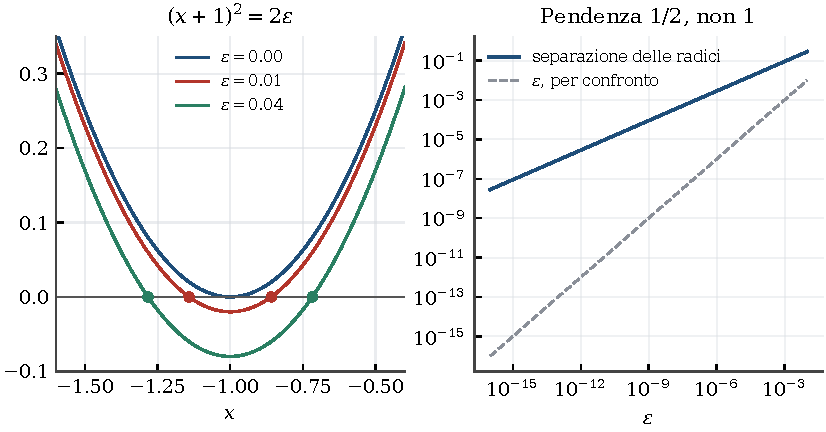
\includegraphics[width=0.86\linewidth]{../figures/teoria_radice_doppia.pdf}
  \caption{Una perturbazione di ampiezza $2\varepsilon$ sul termine noto separa le due radici di $(x+1)^2=0$ di una quantità proporzionale a $\sqrt{\varepsilon}$, non a $\varepsilon$. In scala doppiamente logaritmica la pendenza $1/2$ è la firma della radice doppia.}
  \label{fig:teoria_radice_doppia}
\end{figure}

Il punto è nell'ordine di grandezza. Se il polinomio $(x+1)^2$ viene perturbato di una quantità $2\varepsilon$, le due radici non si spostano di $\varepsilon$: si separano di $2\sqrt{2\varepsilon}$. Con $\varepsilon=10^{-16}$, cioè la precisione di un numero in doppia precisione, la separazione è dell'ordine di $10^{-8}$: otto cifre perse di colpo. È la ragione per cui le radici multiple sono il caso peggiore per qualunque risolutore numerico, ed è notevole vederla isolata così, in quattro righe.

\section{Da dove viene $\varepsilon$}

L'ultima sezione scopre le carte. Il difetto non è un'astrazione: è quello che resta quando si tronca uno sviluppo decimale. Le due espressioni $\#20$ e $\#21$ costruiscono i due protagonisti — un numero fatto di mille cifre $9$ e il prodotto delle potenze successive di $1/10$ — e le successive chiedono quando i due si corrispondano esattamente.

\begin{espr}{20}{User}{}
\[
\mathrm{U} = \sum_{n=0}^{999} 9 \cdot 10^{n}
\]
\end{espr}
Un numero di mille cifre, tutte $9$. La variabile ha un nome non alfabetico, conservato qui come compariva nel file.

\begin{espr}{21}{User}{}
\[
\varepsilon = \prod_{n=1}^{999} \left(\frac{1}{10}\right)^{n}
\]
\end{espr}
Il prodotto vale $10^{-499500}$: un numero minuscolo, il candidato naturale al ruolo di $\varepsilon$.

\begin{espr}{22}{User}{}
\[
\prod_{n=1}^{x} \left(\frac{1}{10}\right)^{n} = \frac{1}{\sum_{n=0}^{x} 9 \cdot 10^{n}}
\]
\end{espr}
L'equazione centrale del quaderno. A sinistra $10^{-x(x+1)/2}$, a destra $1/(10^{x+1}-1)$.

\begin{espr}{23}{Simp(Solve(\#22,x))}{}
\begin{align*}
& 10^{x\, \left(x + 1\right)} - 10^{2\, \left(x + 1\right)} + 2^{x + 2} \cdot 5^{x + 1} = 1 \\[3pt]
\lor\quad & x = \infty + \frac{3\, \pi\, \mathrm{i}}{\ln\!\left(10\right)} \\[3pt]
\lor\quad & x = \infty - \frac{2\, \pi\, \mathrm{i}}{\ln\!\left(10\right)} \\[3pt]
\lor\quad & x = \infty + \frac{2\, \pi\, \mathrm{i}}{\ln\!\left(10\right)} \\[3pt]
\lor\quad & x = \infty - \frac{\pi\, \mathrm{i}}{\ln\!\left(10\right)} \\[3pt]
\lor\quad & x = \infty + \frac{\pi\, \mathrm{i}}{\ln\!\left(10\right)} \\[3pt]
\lor\quad & x = \infty
\end{align*}
\end{espr}
La risposta di Derive: una condizione algebrica più una famiglia di soluzioni all'infinito, generate dalla periodicità immaginaria dell'esponenziale complesso ($2\pi\mathrm{i}/\ln 10$ è il periodo di $10^{z}$).

\begin{espr}{24}{User}{}
\[
10^{x\, \left(x + 1\right)} - 10^{2\, \left(x + 1\right)} + 2^{x + 2} \cdot 5^{x + 1} = 1
\]
\end{espr}
La condizione algebrica isolata. Si ottiene elevando al quadrato $10^{x(x+1)/2}=10^{x+1}-1$; il termine $2^{x+2}5^{x+1}$ non è altro che $2\cdot 10^{x+1}$.

\begin{espr}{25}{Simp(Solve(\#24,x))}{}
\[
x = 1.999710103
\]
\end{espr}
La soluzione numerica: $x$ manca il valore intero $2$ per tre parti su diecimila.

\begin{espr}{26}{Solve(\#22,x)}{}
\[
\operatorname{NSolve}\!\left(\prod_{n=1}^{x} \left(\frac{1}{10}\right)^{n} = \frac{1}{\sum_{n=0}^{x} 9 \cdot 10^{n}},\; x\right)
\]
\end{espr}
La stessa domanda posta al risolutore numerico anziché a quello simbolico.

\begin{espr}{27}{Simp(Solve(\#22,x))}{}
\[
x = 10
\]
\end{espr}
Il valore restituito è $x=10$, che non soddisfa l'equazione: è un artefatto della ricerca numerica, che si è fermata su un punto in cui i due membri sono entrambi enormi e la loro differenza relativa è sotto la soglia di tolleranza. Vale la pena conservarlo come promemoria: un risolutore numerico risponde sempre, anche quando non dovrebbe.


La risposta è il cuore del quaderno. L'equazione $\#22$ si riscrive come $10^{x(x+1)/2}=10^{x+1}-1$: a sinistra una potenza di dieci, a destra una potenza di dieci meno uno. Per $x=2$ i due membri valgono $1000$ e $999$. Non sono uguali — ma lo sono a meno di una parte su mille, e la soluzione numerica $\#25$ lo conferma: $x=1{,}999710\ldots$ invece di $2$. Quel $-1$ che impedisce l'uguaglianza è $\varepsilon$. Tutto il quaderno gira intorno a lui.

\section*{In sintesi}
\addcontentsline{toc}{section}{In sintesi}

Il quaderno non dimostra nulla in senso stretto e non ne ha l'intenzione. Fissa un'intuizione — l'errore come oggetto con leggi proprie — e la mette alla prova su tre fronti: la propagazione nelle potenze, dove trova per via sperimentale i coefficienti binomiali; la sensibilità delle radici multiple, dove ritrova il comportamento $\sqrt{\varepsilon}$ che rende quel caso patologico; e l'origine decimale del difetto, dove $\varepsilon$ si rivela essere il $-1$ di $10^{k}-1$. Delle sei righe sulla propagazione, cinque combaciano con la legge generale e una contiene un refuso: anche questo, in un quaderno sull'errore, ha il suo posto.


%% generato automaticamente da tools/build_tex.py --- non modificare
\chapter{Una costruzione che si dimezza}
\label{cap:teoria2}
\quaderno{teoria2.dfw}{02 Nov 2009}{31}

Novembre 2009. Un quaderno interamente geometrico, e con una struttura ricorsiva che si scopre solo leggendolo fino in fondo. Si parte dalla bisettrice $y=x$ e da una retta perpendicolare; il loro incontro fissa un punto. Per quel punto si fa passare una parabola. Poi si abbassa la retta perpendicolare, si trova un nuovo punto — a metà distanza — e per esso si fa passare una cubica. Poi una quartica. Le ultime tre espressioni chiudono il cerchio con la formula generale per il grado $n$.

\section{Il punto di partenza}

Le prime quattro espressioni fissano la scena. La bisettrice e l'antibisettrice traslata di $k$ si incontrano in un punto che sta a distanza $k/\sqrt{2}$ dall'origine: è il vertice del quadrato di lato $k/2$ costruito sugli assi.

\begin{espr}{1}{User}{}
\[
y = x
\]
\end{espr}
La bisettrice del primo quadrante: sarà il luogo di tutti i punti di appoggio della costruzione.

\begin{espr}{2}{User}{}
\[
y = -x + k
\]
\end{espr}
La retta perpendicolare che stacca sugli assi il segmento $k$.

\begin{espr}{3}{Simp(Solve(User,[x,y]))}{}
\[
\left[\, x = \frac{k}{2} \;\land\; y = \frac{k}{2} \,\right]
\]
\end{espr}
Il loro incontro, ovviamente a metà: entrambe le coordinate valgono $k/2$.

\begin{espr}{4}{User}{}
\[
d = \frac{k}{\sqrt{2}}
\]
\end{espr}
La distanza di quel punto dall'origine, per il teorema di Pitagora sul quadrato di lato $k/2$.

\section{La parabola e il rapporto aureo}

Si cerca ora la parabola $y=ax^2$ che passa per quel punto. Il coefficiente si determina in una riga. Poi si abbassa la retta e si chiede dove incontri la parabola: la risposta contiene una sorpresa.

\begin{espr}{5}{User}{}
\[
y = a\, x^{2}
\]
\end{espr}
Si introduce la famiglia delle parabole per l'origine.

\begin{espr}{6}{User}{}
\[
\frac{k}{2} = a\, \left(\frac{k}{2}\right)^{2}
\]
\end{espr}
Si impone il passaggio per il punto trovato.

\begin{espr}{7}{User}{}
\[
a = \frac{2}{k}
\]
\end{espr}
Il coefficiente che ne risulta.

\begin{espr}{8}{User}{}
\[
y = \frac{2}{k}\, x^{2}
\]
\end{espr}
La parabola determinata. Con $k=1$ diventa $y=2x^2$.

\begin{espr}{9}{User}{}
\[
y = -x + \frac{k}{2}
\]
\end{espr}
La retta si abbassa: il termine noto passa da $k$ a $k/2$.

\begin{espr}{10}{User}{}
\[
x = k\, \left(\frac{\sqrt{5}}{4} - \frac{1}{4}\right) \;\land\; y = k\, \left(\frac{3}{4} - \frac{\sqrt{5}}{4}\right)
\]
\end{espr}
L'intersezione della parabola con la retta abbassata, dove compare $\sqrt5$.

\begin{espr}{11}{User}{}
\[
\left[\, x = \frac{k}{4} \;\land\; y = \frac{k}{4} \,\right]
\]
\end{espr}
L'intersezione della retta abbassata con la bisettrice: il nuovo punto di appoggio, a coordinate $k/4$. È questo, non il precedente, a generare il passo successivo.


L'ascissa dell'intersezione, $\#10$, vale $k(\sqrt5-1)/4$. Il fattore $(\sqrt5-1)/2$ è l'inverso del rapporto aureo, $1/\varphi\approx 0{,}618$: la parabola taglia la retta abbassata in un punto che divide il segmento in proporzione aurea. Non è una coincidenza costruita apposta — emerge dall'equazione $2x^2+kx-k^2/2=0$, il cui discriminante è $5k^2$. Il quaderno non commenta il fatto e passa oltre.

\section{La cubica}

Il punto $\#11$, che sta a metà strada rispetto al precedente, diventa il nuovo appoggio: per esso passa una cubica. La struttura del passaggio è identica a quella della parabola, e questo è il segnale che si tratta di una ricorsione.

\begin{espr}{12}{User}{}
\[
y = a\, x^{3}
\]
\end{espr}
La famiglia delle cubiche.

\begin{espr}{13}{User}{}
\[
\frac{k}{4} = a\, \left(\frac{k}{4}\right)^{3}
\]
\end{espr}
Il passaggio imposto per il punto a coordinate $k/4$.

\begin{espr}{14}{User}{}
\[
a = \frac{16}{k^{2}}
\]
\end{espr}
Il coefficiente: $16/k^2$, cioè $2^4$ diviso $k^2$.

\begin{espr}{15}{User}{}
\[
y = \frac{16}{k^{2}}\, x^{3}
\]
\end{espr}
La cubica determinata.

\begin{espr}{16}{User}{}
\[
y = -x + \frac{k}{4}
\]
\end{espr}
La retta si abbassa ancora, a $k/4$.

\begin{espr}{17}{Simp(User)}{}
\[
x = k\, \left(\left(\frac{\sqrt{93}}{1152} + \frac{1}{128}\right)^{\frac{1}{3}} - \left(\frac{\sqrt{93}}{1152} - \frac{1}{128}\right)^{\frac{1}{3}}\right) \;\land\; y = k\, \left(\left(\frac{\sqrt{93}}{1152} - \frac{1}{128}\right)^{\frac{1}{3}} - \left(\frac{\sqrt{93}}{1152} + \frac{1}{128}\right)^{\frac{1}{3}} + \frac{1}{4}\right)
\]
\end{espr}
L'intersezione, in forma di Cardano. I due radicandi differiscono solo per il segno del termine $1/128$, come è tipico della formula risolutiva del terzo grado.


L'espressione $\#17$ è la soluzione di Cardano dell'equazione $16x^3+x-k/4=0$: due radici cubiche di binomi che contengono $\sqrt{93}$. Il contrasto con il caso quadratico è istruttivo — stessa costruzione, un grado in più, e la soluzione passa da $\sqrt5$ a una forma irriducibile in radicali annidati.

\section{I casi particolari con $k=1$}

Una breve pausa di verifica: le stesse curve e le stesse rette scritte con $k=1$, per poterle disegnare. Sono le espressioni che il quaderno mandava alla finestra grafica.

\begin{espr}{18}{User}{}
\[
y = 16\, x^{3}
\]
\end{espr}
La cubica con $k=1$.

\begin{espr}{19}{User}{}
\[
y = -x + \frac{1}{4}
\]
\end{espr}
La retta corrispondente, pronta per il grafico.

\begin{espr}{20}{User}{}
\[
y = 2\, x^{2}
\]
\end{espr}
La parabola con $k=1$.

\begin{espr}{21}{User}{}
\[
y = -x + \frac{1}{2}
\]
\end{espr}
La sua retta.

\begin{espr}{22}{User}{}
\[
y = x
\]
\end{espr}
La bisettrice, che nella costruzione è la curva di grado uno.

\begin{espr}{23}{User}{}
\[
y = -x + 1
\]
\end{espr}
E la retta di partenza, con $k=1$: il caso $n=1$ della famiglia generale.

\section{La quartica e la legge generale}

L'ultimo giro della ricorsione, e poi la formula che li racchiude tutti.

\begin{espr}{24}{User}{}
\[
y = a\, x^{4}
\]
\end{espr}
Si passa al quarto grado.

\begin{espr}{25}{User}{}
\[
\frac{k}{8} = a\, \left(\frac{k}{8}\right)^{4}
\]
\end{espr}
Il punto di appoggio è ora a coordinate $k/8$: ogni passo dimezza.

\begin{espr}{26}{User}{}
\[
a = \frac{512}{k^{3}}
\]
\end{espr}
Il coefficiente $512=2^9$.

\begin{espr}{27}{User}{}
\[
y = \frac{512}{k^{3}}\, x^{4}
\]
\end{espr}
La quartica determinata.

\begin{espr}{28}{User}{}
\[
y = -x + \frac{1}{8}
\]
\end{espr}
La retta corrispondente.

\begin{espr}{29}{User}{}
\[
a = \frac{2^{\left(n - 1\right)^{2}}}{k^{n - 1}}
\]
\end{espr}
La legge generale del coefficiente. L'esponente $(n-1)^2$ dà $2^0,\ 2^1,\ 2^4,\ 2^9,\ 2^{16}$ per $n=1,2,3,4,5$.

\begin{espr}{30}{User}{}
\[
y = \frac{2^{\left(n - 1\right)^{2}}}{k^{n - 1}}\, x^{n}
\]
\end{espr}
La famiglia completa di curve.

\begin{espr}{31}{User}{}
\[
y = -x + 2^{1 - n}
\]
\end{espr}
E la famiglia di rette che le accompagna. Il termine noto $2^{1-n}$ genera il punto di appoggio del grado successivo, non di quello corrente: è questo sfasamento a rendere la costruzione una ricorsione anziché una semplice sostituzione.

\begin{figure}[htbp]
  \centering
  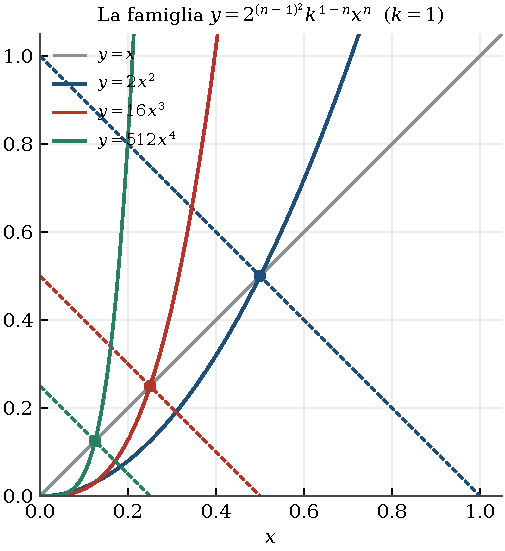
\includegraphics[width=0.66\linewidth]{../figures/teoria2.pdf}
  \caption{La costruzione con $k=1$. Ogni curva incontra la bisettrice in un punto che dista dall'origine la metà del precedente; la retta tratteggiata dello stesso colore è quella che ha generato il punto di appoggio.}
  \label{fig:teoria2}
\end{figure}

La formula $\#29$ è il punto di arrivo. Il coefficiente $a=2^{(n-1)^2}k^{1-n}$ è esattamente quello che serve perché la curva $y=ax^n$ passi per il punto $\left(k/2^{\,n-1},\ k/2^{\,n-1}\right)$: imponendo $p=ap^n$ con $p=k/2^{\,n-1}$ si ricava $a=p^{1-n}$, e sviluppando la potenza compare l'esponente quadratico $(n-1)^2$. La crescita è impressionante: $2$, $16$, $512$, $65\,536$, e al passo successivo già oltre trentatré milioni. Ogni grado in più costringe la curva a stare più aderente all'asse per poi risalire fino alla bisettrice in un punto due volte più vicino all'origine.

\section*{In sintesi}
\addcontentsline{toc}{section}{In sintesi}

Trentuno espressioni per una sola idea, sviluppata con pazienza: una successione di curve di grado crescente ancorate a punti che si avvicinano geometricamente all'origine. Il risultato finale, $a=2^{(n-1)^2}k^{1-n}$, è compatto e si verifica in una riga; ma il modo in cui il quaderno ci arriva — un caso, poi un altro, poi un terzo, e solo allora la formula — è il modo in cui le regolarità si trovano davvero.


%% generato automaticamente da tools/build_tex.py --- non modificare
\chapter{Una riga sola}
\label{cap:limit}
\quaderno{limit.dfw}{19 Dec 2009}{1}

Dicembre 2009. Il quaderno più breve della raccolta contiene una sola espressione, e non è un calcolo: è una maggiorazione. Merita un capitolo proprio perché mostra bene che cosa fossero questi file — non solo un blocco per appunti di calcolo, ma anche un posto dove fissare una disuguaglianza che era servita e che si voleva ritrovare.

\section{La disuguaglianza}
\begin{espr}{1}{User}{}
\[
\left|x\right| \leq \frac{\sqrt{2}}{2}\, \left(\frac{1}{2} + x^{2}\right)
\]
\end{espr}
A sinistra una funzione non derivabile nell'origine, a destra una parabola. La parabola sta sempre sopra e la tocca in due punti simmetrici.

\begin{figure}[htbp]
  \centering
  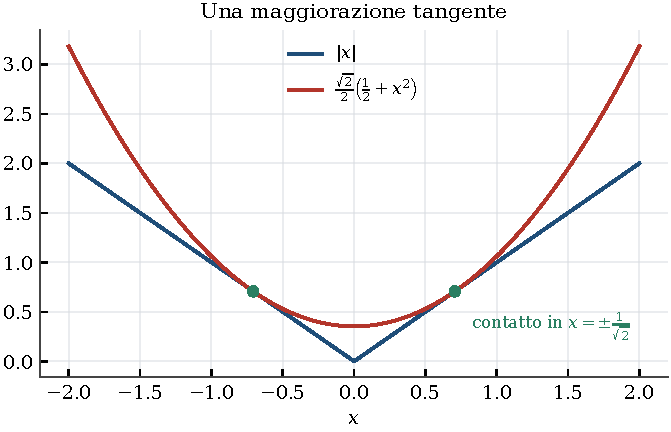
\includegraphics[width=0.86\linewidth]{../figures/limit_disug.pdf}
  \caption{La parabola $\tfrac{\sqrt2}{2}\left(\tfrac12+x^2\right)$ domina $|x|$ su tutta la retta e la tocca nei due punti $x=\pm1/\sqrt2$. La costante $\sqrt2/2$ è la più piccola per cui questo accade.}
  \label{fig:limit_disug}
\end{figure}

La disuguaglianza è vera per ogni $x$ reale e si dimostra in una riga con la media aritmetico-geometrica. Da $\left(|x|-\tfrac{1}{\sqrt2}\right)^2\geq 0$ segue $x^2+\tfrac12\geq \sqrt2\,|x|$, e moltiplicando per $\tfrac{\sqrt2}{2}$ si ottiene esattamente il secondo membro. L'uguaglianza vale nei due punti $x=\pm 1/\sqrt2$, dove la parabola è tangente alle due semirette che compongono $|x|$.

Il motivo per cui una maggiorazione di questo tipo è utile si legge nella costante: $\sqrt2/2$ è il valore più piccolo possibile. Qualunque disuguaglianza della forma $|x|\leq c\left(\tfrac12+x^2\right)$ valida su tutto $\mathbb{R}$ richiede $c\geq\sqrt2/2$, perché il rapporto $|x|/(\tfrac12+x^2)$ ha massimo $\sqrt2/2$ proprio in $x=\pm1/\sqrt2$. La costante non è scelta per comodità: è ottima.


%% generato automaticamente da tools/build_tex.py --- non modificare
\chapter{Novantatré modi di guardare $\mathrm{e}$}
\label{cap:e}
\quaderno{e.dfw}{27 Aug 2010}{93}

Agosto 2010, il quaderno più lungo dopo i due gemelli su trigonometria. È una lunga esplorazione attorno al numero di Nepero, condotta con un metodo preciso: prendere la definizione classica $\left(1+\tfrac1x\right)^x$ e romperla in tutti i modi possibili per vedere che cosa resiste. Alcune modifiche distruggono il limite, altre lo lasciano intatto, altre ancora lo spostano in modo controllato. Alla fine il quaderno arriva, senza dichiararlo, alla formula di Eulero.

\section{Che cosa succede se si sottrae un infinitesimo}

Le prime espressioni introducono una perturbazione $\varepsilon$ nella base del limite fondamentale. È lo stesso $\varepsilon$ del quaderno del 2009 (capitolo~\ref{cap:teoria}), qui messo alla prova su un limite notevole.

\begin{espr}{1}{Lim(User,x)}{}
\[
\lim_{x \to \infty} \left(1 + \frac{1}{x} - \varepsilon\right)^{x}
\]
\end{espr}
La base tende a $1-\varepsilon$, un numero minore di uno; elevato a un esponente che diverge, il risultato collassa.

\begin{espr}{2}{Simp(Lim(User,x))}{}
\[
\infty^{\ln\!\left(1 - \varepsilon\right)}
\]
\end{espr}
La scrittura di Derive è formale ma corretta nel segno: $\ln(1-\varepsilon)$ è negativo, e $\infty$ elevato a un esponente negativo vale zero.

\begin{espr}{3}{User}{}
\[
\lim_{x \to \infty} \left(1 + \frac{1}{x} - \frac{1}{99999999999\, x}\right)^{x}
\]
\end{espr}
Ora la perturbazione decresce come $1/x$: è dello stesso ordine del termine che genera $\mathrm{e}$, e quindi conta.

\begin{espr}{4}{Simp(\#3)}{}
\[
\mathrm{e}^{\frac{99999999998}{99999999999}}
\]
\end{espr}
Il risultato è $\mathrm{e}$ elevato a un esponente pochissimo minore di uno.

\begin{espr}{5}{User}{}
\[
\lim_{x \to \infty} \left(1 + \frac{1}{x} - \frac{1}{k\, x}\right)^{x}
\]
\end{espr}
La stessa cosa con un parametro generico al posto del numero di undici cifre.

\begin{espr}{6}{Simp(\#5)}{}
\[
\mathrm{e}^{1 - \frac{1}{k}}
\]
\end{espr}
La formula generale: $\mathrm{e}^{1-1/k}$. Per $k=1$ vale $1$, per $k\to\infty$ tende a $\mathrm{e}$.

\begin{espr}{7}{Lim(User,}{}
\[
\lim_{\varepsilon \to 0} \left(1 + \frac{1}{k\, \varepsilon} - \varepsilon\right)^{\frac{1}{k\, \varepsilon}}
\]
\end{espr}
Si scambiano i ruoli: ora è $\varepsilon$ a tendere a zero e a comparire anche nell'esponente.

\begin{espr}{8}{Simp(\#7)}{}
\[
\mathrm{?}
\]
\end{espr}
Derive non conclude: il punto interrogativo è la sua risposta quando la forma è indeterminata.

\begin{espr}{9}{User}{}
\[
\lim_{\varepsilon \to 0} \left(1 + \frac{1}{\varepsilon} - \varepsilon\right)^{\frac{1}{\varepsilon}}
\]
\end{espr}
Variante senza il parametro $k$.

\begin{espr}{10}{Simp(\#9)}{}
\[
\mathrm{?}
\]
\end{espr}
Ancora indeterminato.

\begin{espr}{11}{User}{}
\[
\lim_{\varepsilon \to 0} \left(\frac{1}{\varepsilon}\right)^{\ln\!\left(1 - \varepsilon\right)}
\]
\end{espr}
Una forma più semplice della stessa famiglia, questa volta trattabile.

\begin{espr}{12}{Simp(\#11)}{}
\[
1
\]
\end{espr}
Il limite vale $1$: infatti $\ln(1-\varepsilon)\approx-\varepsilon$, e $(1/\varepsilon)^{-\varepsilon}=\mathrm{e}^{-\varepsilon\ln(1/\varepsilon)}\to1$.

\begin{espr}{13}{User}{}
\[
\lim_{x \to \infty} \left(\varepsilon\, x + \frac{1}{x} - \varepsilon\right)^{x}
\]
\end{espr}
Qui $\varepsilon$ moltiplica $x$: la base diverge invece di tendere a uno.

\begin{espr}{14}{Simp(\#13)}{}
\[
\mathbb{S}^{1}\, \infty
\]
\end{espr}
La risposta di Derive dice due cose: il modulo è infinito e la fase è indeterminata. $\mathtt{unit\_circle}$ è il modo del programma di indicare un argomento qualsiasi.


Il risultato di questo primo gruppo è che $\varepsilon$ e $1/x$ non sono intercambiabili. Se la perturbazione è una costante, per quanto piccola, la base tende a $1-\varepsilon<1$ e la potenza $x$-esima annulla tutto. Se invece la perturbazione decresce come $1/x$ — cioè allo stesso ordine del termine che genera $\mathrm{e}$ — il limite resta finito e vale $\mathrm{e}^{1-1/k}$. Fissato $k$, si ottiene un'intera famiglia di valori che interpola fra $1$ e $\mathrm{e}$: per $k=1$ la perturbazione cancella esattamente il termine $1/x$ e il limite è $1$; per $k\to\infty$ si ritrova $\mathrm{e}$.

\section{Aggiungere termini non cambia nulla}

Domanda opposta: e se invece di togliere si aggiunge? Le espressioni seguenti mettono nella base non solo $1/x$ ma anche $1/x^2$, $1/x^3$, e infine tutta la serie geometrica.

\begin{espr}{15}{User}{}
\[
\lim_{x \to \infty} \left(1 + \frac{1}{x} + \frac{1}{x^{2}}\right)^{x}
\]
\end{espr}
Si aggiunge un termine di ordine $1/x^2$.

\begin{espr}{16}{Simp(\#15)}{}
\[
\mathrm{e}
\]
\end{espr}
Il limite non cambia.

\begin{espr}{17}{User}{}
\[
\lim_{x \to \infty} \left(1 + \frac{1}{x} + \frac{1}{x^{2}} + \frac{1}{x^{3}} + \frac{1}{x^{4}}\right)^{x}
\]
\end{espr}
Se ne aggiungono altri due.

\begin{espr}{18}{Simp(\#17)}{}
\[
\mathrm{e}
\]
\end{espr}
Ancora $\mathrm{e}$.

\begin{espr}{19}{Lim(User,x)}{}
\[
\lim_{x \to \infty} \left(\sum_{n=0}^{\infty} \frac{1}{x^{n}}\right)^{x}
\]
\end{espr}
Il caso limite: tutta la serie geometrica $\sum_{n\ge0}x^{-n}$.

\begin{espr}{20}{User}{}
\[
\lim_{x \to \infty} \left(\sum_{n=0}^{9} \frac{1}{x^{n}}\right)^{x}
\]
\end{espr}
Troncata a dieci termini.

\begin{espr}{21}{User}{}
\[
\lim_{x \to \infty} \left(\sum_{n=0}^{99} \frac{1}{x^{n}}\right)^{x}
\]
\end{espr}
Troncata a cento.

\begin{espr}{22}{Simp(\#21)}{}
\[
\mathrm{e}
\]
\end{espr}
Il valore è sempre lo stesso, e si capisce perché: solo il primo termine oltre l'unità sopravvive al limite.


Il limite non si muove: resta $\mathrm{e}$. La ragione è che solo il termine di ordine $1/x$ conta. Se la base è $1+\tfrac1x+O\!\left(\tfrac{1}{x^2}\right)$, il logaritmo vale $\tfrac1x+O\!\left(\tfrac{1}{x^2}\right)$ e moltiplicato per $x$ tende a $1$. Tutto ciò che decresce più in fretta di $1/x$ è invisibile al limite. È il complemento esatto della sezione precedente: là una perturbazione troppo lenta distruggeva il limite, qui una troppo rapida non lo tocca.

\section{Il rischio di sostituire un valore finito}

Un intermezzo che vale come avvertimento. Che cosa succede se in una formula pensata per $x$ grande si sostituisce un valore concreto?

\begin{espr}{23}{User}{}
\[
\left(1 + \frac{1}{100} - 100\right)^{\frac{1}{100}}
\]
\end{espr}
Che cosa dà la formula se si mette $x=100$ dentro una scrittura pensata per $x\to\infty$.

\begin{espr}{24}{Simp(\#23)}{}
\[
\left(\frac{9899}{100}\right)^{\frac{1}{100}}\, \left(-1\right)^{\frac{1}{100}}
\]
\end{espr}
La base è negativa: Derive isola il fattore $(-1)^{1/100}$.

\begin{espr}{25}{User}{}
\[
\left(1 + \frac{1}{999} - 999\right)^{\frac{1}{999}}
\]
\end{espr}
Stessa prova con $x=999$.

\begin{espr}{26}{Simp(\#25)}{}
\[
\left(\frac{997001}{999}\right)^{\frac{1}{999}}\, \left(-1\right)^{\frac{1}{999}}
\]
\end{espr}
Stessa struttura.

\begin{espr}{27}{Approx(\#26)}{}
\[
1.006931633 + 0.003166545996\, \mathrm{i}
\]
\end{espr}
Il valore numerico è complesso, con parte immaginaria piccola ma non nulla: è la determinazione principale della radice centesima di un numero negativo.


La base diventa negativa e la potenza frazionaria esce dai reali. Derive, che lavora con la determinazione principale, restituisce correttamente un numero complesso. Non è un errore del programma: è quello che accade quando si prende una formula asintotica e la si valuta fuori dal suo regime.

\section{Troncare la serie all'indice variabile}

Variante più sottile: sommare la serie geometrica non fino all'infinito ma fino a $n=x$, cioè con un numero di termini che cresce insieme alla variabile.

\begin{espr}{28}{User}{}
\[
\left(\sum_{n=0}^{\infty} \frac{1}{x^{n}}\right)^{x} = \mathrm{e}
\]
\end{espr}
L'affermazione che il quaderno vuole verificare: la serie geometrica al posto del binomio dà ancora $\mathrm{e}$.

\begin{espr}{29}{User}{}
\[
\lim_{x \to \infty} \left(\sum_{n=0}^{x} \frac{1}{x^{n}}\right)^{x}
\]
\end{espr}
Variante con l'estremo superiore della somma legato alla variabile.

\begin{espr}{30}{Simp(User)}{}
\[
1
\]
\end{espr}
\begin{espr}{31}{User}{}
\[
\left(\sum_{n=0}^{x} \frac{1}{x^{n}}\right)^{x}
\]
\end{espr}
La somma parziale scritta esplicitamente.

\begin{espr}{32}{Simp(\#31)}{}
\[
\left(\frac{x^{-x}\, \left(x^{x + 1} - 1\right)}{x - 1}\right)^{x}
\]
\end{espr}
La sua forma chiusa: somma di una geometrica di ragione $1/x$ con $x+1$ termini.

\begin{espr}{33}{Lim(\#32,x)}{}
\[
\lim_{x \to \mathrm{e}} \left(\frac{x^{-x}\, \left(x^{x + 1} - 1\right)}{x - 1}\right)^{x}
\]
\end{espr}
Valutata in $x=\mathrm{e}$.

\begin{espr}{34}{Approx(\#33)}{}
\[
3.254394129
\]
\end{espr}
Circa $3{,}2544$.

\begin{espr}{35}{Lim(\#32,x)}{}
\[
\lim_{x \to \pi} \left(\frac{x^{-x}\, \left(x^{x + 1} - 1\right)}{x - 1}\right)^{x}
\]
\end{espr}
Valutata in $x=\pi$.

\begin{espr}{36}{Approx(User)}{}
\[
3.24219215
\]
\end{espr}
Circa $3{,}2422$. I due valori sono vicini fra loro ma non a $\mathrm{e}$: il troncamento all'indice $x$ cambia la natura del limite.


La forma chiusa $\#32$ è la somma di una progressione geometrica di ragione $1/x$ con $x+1$ termini. Valutata nei due punti notevoli $x=\mathrm{e}$ e $x=\pi$ dà due numeri vicini fra loro e vicini a $\pi$, ma senza un significato particolare: sono le prime due tacche di una curva che il quaderno non prosegue.

\section{La parabola che ha per radici $\mathrm{e}$ e $\pi$}

Cambio di scena. Si costruisce il polinomio di secondo grado più semplice che si annulla nei due numeri, e se ne studiano vertice e integrale.

\begin{espr}{37}{User}{}
\[
y = x^{2} - \left(\pi + \mathrm{e}\right)\, x + \pi\, \mathrm{e}
\]
\end{espr}
Il polinomio di secondo grado con radici $\mathrm{e}$ e $\pi$, scritto per somma e prodotto delle radici.

\begin{espr}{38}{User}{}
\[
x^{2} - \left(\pi + \mathrm{e}\right)\, x + \pi\, \mathrm{e} = 0
\]
\end{espr}
La stessa cosa come equazione.

\begin{espr}{39}{Simp(Solve(\#38,x))}{}
\[
x = \mathrm{e} \;\lor\; x = \pi
\]
\end{espr}
Derive conferma le due radici.

\begin{espr}{40}{Dif(\#37,x)}{}
\[
\frac{\mathrm{d}}{\mathrm{d}x}\!\left[y = x^{2} - \left(\pi + \mathrm{e}\right)\, x + \pi\, \mathrm{e}\right]
\]
\end{espr}
Si deriva per cercare il vertice.

\begin{espr}{41}{Simp(Solve(User,x))}{}
\[
x = \frac{\mathrm{e} + \pi}{2}
\]
\end{espr}
L'ascissa del vertice è la media dei due numeri, $\approx 2{,}930$.

\begin{espr}{42}{User}{}
\[
y = -\frac{\left(\mathrm{e} - \pi\right)^{2}}{4}
\]
\end{espr}
L'ordinata del vertice: metà differenza al quadrato, cambiata di segno.

\begin{espr}{43}{User}{}
\[
\int_{\pi}^{\mathrm{e}} x^{2} - \left(\pi + \mathrm{e}\right)\, x + \pi\, \mathrm{e} \,\mathrm{d}x
\]
\end{espr}
L'integrale fra le due radici, percorso da $\pi$ verso $\mathrm{e}$.

\begin{espr}{44}{User}{}
\[
\frac{\left(\pi - \mathrm{e}\right)^{3}}{3!}
\]
\end{espr}
Il valore, in forma notevole: la differenza al cubo divisa per $3!$.

\begin{espr}{45}{Approx(User)}{}
\[
0.01264232275
\]
\end{espr}
Numericamente circa $0{,}01264$.

\begin{figure}[htbp]
  \centering
  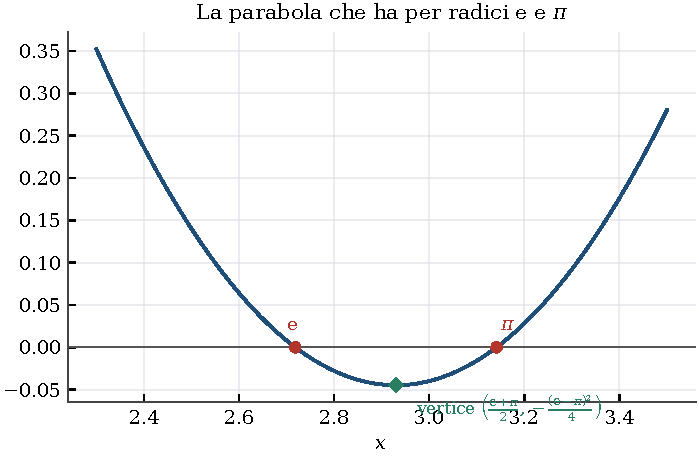
\includegraphics[width=0.86\linewidth]{../figures/e_parabola.pdf}
  \caption{La parabola $x^2-(\pi+\mathrm{e})x+\pi\mathrm{e}$. L'area fra la curva e l'asse, fra le due radici, vale $(\pi-\mathrm{e})^3/3!$ percorsa da $\pi$ verso $\mathrm{e}$.}
  \label{fig:e_parabola}
\end{figure}
\begin{espr}{46}{User}{}
\[
\frac{\left(\pi - \mathrm{e}\right)^{n}}{n!}
\]
\end{espr}
Il termine generale di una serie esponenziale suggerita dalla forma precedente.

\begin{espr}{47}{Sum(\#46,n)}{}
\[
\sum_{n=0}^{+\infty} \frac{\left(\pi - \mathrm{e}\right)^{n}}{n!}
\]
\end{espr}
La sua somma.

\begin{espr}{48}{Simp(\#47)}{}
\[
\mathrm{e}^{\pi - \mathrm{e}}
\]
\end{espr}
Che vale $\mathrm{e}^{\pi-\mathrm{e}}$.

\begin{espr}{49}{Approx(\#48)}{}
\[
1.527008854
\]
\end{espr}
Circa $1{,}527$.


L'integrale $\#43$ ha un valore notevole. Per un polinomio $(x-a)(x-b)$ si ha sempre $\int_a^b (x-a)(x-b)\,\mathrm{d}x=-\tfrac{(b-a)^3}{6}$, e qui, integrando da $\pi$ a $\mathrm{e}$ cioè nel verso che rovescia il segno, si ottiene esattamente $(\pi-\mathrm{e})^3/3!$. Il fattoriale al denominatore suggerisce il passo successivo, che il quaderno compie subito dopo: se $(\pi-\mathrm{e})^3/3!$ è il termine di indice tre di una serie esponenziale, sommiamo tutti gli altri. Il risultato è $\mathrm{e}^{\pi-\mathrm{e}}\approx 1{,}527$.

\section{Equazioni che legano i due numeri}

Una sequenza di piccole equazioni in cui $\mathrm{e}$ e $\pi$ si scambiano i ruoli di base e di esponente. Le ultime quattro producono un accostamento numerico che vale la pena di seguire.

\begin{espr}{50}{User}{\verificata}
\[
\lim_{n \to \infty} \left(1 + \frac{1}{n}\right)^{n} = \sum_{n=0}^{\infty} \frac{1}{n!}
\]
\end{espr}
Le due definizioni classiche di $\mathrm{e}$ affiancate: il limite e la serie.

\begin{espr}{51}{User}{}
\[
\left(x + \frac{1}{\sum_{n=0}^{\infty} n!}\right)^{\sum_{n=0}^{\infty} n!} = \sum_{n=0}^{\infty} \frac{1}{n!}
\]
\end{espr}
Una scrittura formale in cui compare $\sum n!$, che diverge. È un appunto, non un'identità: il quaderno sta cercando che cosa si possa mettere al posto dell'esponente.

\begin{espr}{52}{User}{}
\[
\left(x + \frac{1}{\pi}\right)^{\pi} = \mathrm{e}
\]
\end{espr}
Un'equazione concreta della stessa famiglia, con $\pi$ all'esponente.

\begin{espr}{53}{Simp(Solve(\#52,x))}{}
\[
x = \mathrm{e}^{\frac{1}{\pi}} - \frac{1}{\pi}
\]
\end{espr}
La sua soluzione.

\begin{espr}{54}{User}{}
\[
\left(1 + \frac{1}{x}\right)^{\pi} = \mathrm{e}
\]
\end{espr}
Variante: l'incognita passa dalla base al denominatore.

\begin{espr}{55}{Simp(Solve(\#54,x))}{}
\[
x = \frac{1}{\mathrm{e}^{\frac{1}{\pi}} - 1}
\]
\end{espr}
La soluzione corrispondente.

\begin{espr}{56}{User}{}
\[
\mathrm{e}^{\pi} - \mathrm{e}^{3}
\]
\end{espr}
Confronto fra $\mathrm{e}^{\pi}$ e $\mathrm{e}^3$, cioè fra $\pi$ e $3$ all'esponente.

\begin{espr}{57}{Approx(\#56)}{}
\[
3.055155709
\]
\end{espr}
Circa $3{,}055$.

\begin{espr}{58}{User}{}
\[
\mathrm{e}^{\pi} - \pi^{\mathrm{e}}
\]
\end{espr}
Il classico confronto fra $\mathrm{e}^{\pi}$ e $\pi^{\mathrm{e}}$.

\begin{espr}{59}{Approx(User)}{}
\[
0.6815349142
\]
\end{espr}
La differenza è positiva: $\mathrm{e}^{\pi}>\pi^{\mathrm{e}}$, come è noto.

\begin{espr}{60}{Simp(Solve(User,x))}{}
\[
x = \pi^{\mathrm{e}}\, \mathrm{e}^{-\pi}
\]
\end{espr}
Il loro rapporto, scritto come soluzione di un'equazione.

\begin{espr}{61}{User}{}
\[
x\, \mathrm{e}^{\pi} - \pi^{\mathrm{e}} = 0
\]
\end{espr}
L'equazione che lo definisce.

\begin{espr}{62}{Approx(\#60)}{}
\[
x = 0.9705482059
\]
\end{espr}
Il rapporto vale $0{,}97055$.

\begin{espr}{63}{User}{}
\[
\mathrm{e}^{\pi} - x\, \pi^{\mathrm{e}} = 0
\]
\end{espr}
L'equazione reciproca.

\begin{espr}{64}{Simp(Solve(\#63,x))}{}
\[
x = \pi^{-\mathrm{e}}\, \mathrm{e}^{\pi}
\]
\end{espr}
Il rapporto inverso.

\begin{espr}{65}{Approx(\#64)}{}
\[
x = 1.030345524
\]
\end{espr}
Che vale $1{,}03035$.

\begin{espr}{66}{User}{}
\[
\frac{\pi^{\mathrm{e}}\, \mathrm{e}^{-\pi} + \pi^{-\mathrm{e}}\, \mathrm{e}^{\pi}}{2}
\]
\end{espr}
La semisomma dei due rapporti: un coseno iperbolico.

\begin{espr}{67}{Approx(User)}{}
\[
1.000446865
\]
\end{espr}
Vale $1{,}000447$, cioè quasi esattamente uno.

\begin{espr}{68}{User}{}
\[
\frac{-\pi^{\mathrm{e}}\, \mathrm{e}^{-\pi} + \pi^{-\mathrm{e}}\, \mathrm{e}^{\pi}}{2}
\]
\end{espr}
La semidifferenza: il seno iperbolico corrispondente.

\begin{espr}{69}{Approx(\#68)}{}
\[
0.02989865915
\]
\end{espr}
Vale $0{,}0298987$. Da confrontare con il capitolo~\ref{cap:sin-cos}.


Le espressioni $\#66$ e $\#68$ costruiscono la semisomma e la semidifferenza di $\pi^{-\mathrm{e}}\mathrm{e}^{\pi}$ e del suo reciproco. Qui conviene dare un nome alla quantità $k=\pi-\mathrm{e}\ln\pi$, perché $\pi^{-\mathrm{e}}\mathrm{e}^{\pi}=\mathrm{e}^{\pi-\mathrm{e}\ln\pi}=\mathrm{e}^{k}$: le due espressioni sono allora, esattamente, $\cosh k$ e $\sinh k$.

Questo spiega il valore $0{,}029898659\ldots$ della riga $\#69$, e spiega perché somigli tanto a $k=0{,}029894206\ldots$ senza coincidervi: $\sinh k-k=k^3/6\approx 4{,}45\cdot10^{-6}$, che è esattamente lo scarto osservato. Non è una coincidenza numerica ma un'identità, e il quaderno \dfw{sin-cos.dfw} del gennaio precedente (capitolo~\ref{cap:sin-cos}) la sviluppa per intero: là si scopre che $k$ è la pulsazione di un intero sistema di funzioni iperboliche costruito su $\pi$ ed $\mathrm{e}$.

\section{Una successione che converge molto più in fretta}

Ritorno al tema centrale, con un'idea nuova: sommare $n^{-k}$ per $k$ da $0$ a $n$, ed elevare alla $n$.

\begin{espr}{70}{User}{}
\[
\lim_{n \to \infty} \left(\sum_{k=0}^{n} \frac{1}{n^{k}}\right)^{n}
\]
\end{espr}
La successione più rapida: somma di $n^{-k}$ per $k$ fino a $n$, elevata a $n$.

\begin{espr}{71}{Simp(User)}{}
\[
1
\]
\end{espr}
\begin{espr}{72}{User}{}
\[
\lim_{n \to 9999999} \left(\sum_{k=0}^{n} \frac{1}{n^{k}}\right)^{n}
\]
\end{espr}
Valutata in $n=10^7-1$.

\begin{espr}{73}{Approx(\#72)}{}
\[
2.718281964
\]
\end{espr}
Il risultato ha sette cifre esatte di $\mathrm{e}$.

\begin{espr}{74}{User}{}
\[
\lim_{n \to 9999999} \left(\sum_{k=0}^{n} \frac{1}{n^{k}}\right)^{n} - \mathrm{e}
\]
\end{espr}
La differenza dal valore vero.

\begin{espr}{75}{Approx(\#74)}{}
\[
1.359141174 \cdot 10^{-7}
\]
\end{espr}
Poco più di un decimilionesimo.

\begin{figure}[htbp]
  \centering
  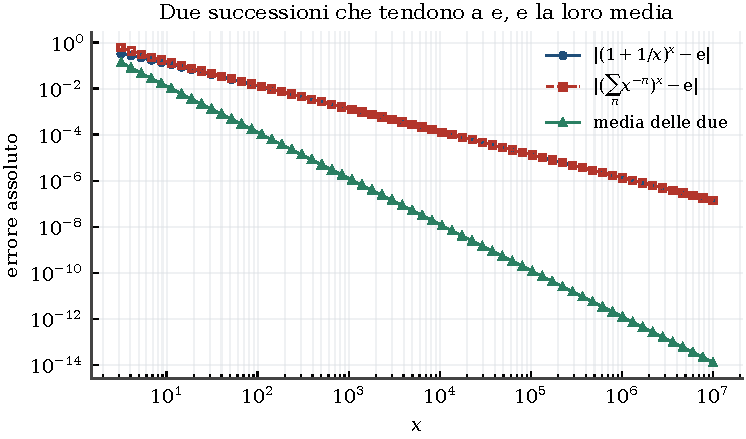
\includegraphics[width=0.86\linewidth]{../figures/e_convergenza.pdf}
  \caption{Errore assoluto delle due successioni al variare di $x$, in scala doppiamente logaritmica. La successione classica scende con pendenza $-1$; quella costruita sulla serie geometrica è di gran lunga più rapida.}
  \label{fig:e_convergenza}
\end{figure}
\begin{espr}{76}{User}{}
\[
\sum_{n=0}^{\infty} \left(\frac{1}{x}\right)^{n} = \frac{x}{x - 1}
\]
\end{espr}
La somma della serie geometrica in forma chiusa.

\begin{espr}{77}{User}{\verificata}
\[
\lim_{x \to +\infty} \left(\frac{x}{x - 1}\right)^{x} = \mathrm{e}
\]
\end{espr}
Il limite per $x\to+\infty$ vale $\mathrm{e}$.

\begin{espr}{78}{User}{\verificata}
\[
\lim_{x \to -\infty} \left(\frac{x}{x - 1}\right)^{x} = \mathrm{e}
\]
\end{espr}
E anche per $x\to-\infty$: la funzione $\left(\tfrac{x}{x-1}\right)^x$ tende a $\mathrm{e}$ da entrambe le parti.

\begin{espr}{79}{User}{}
\[
\left(1 + \frac{1}{x}\right)^{x}
\]
\end{espr}
La successione classica, per confronto.

\begin{espr}{80}{User}{\verificata}
\[
\lim_{x \to -\infty} \left(1 + \frac{1}{x}\right)^{x} = \mathrm{e}
\]
\end{espr}
Che ha la stessa proprietà: il limite da $-\infty$ è ancora $\mathrm{e}$.

\begin{espr}{81}{User}{\verificata}
\[
\lim_{x \to +\infty} \left(\sum_{n=0}^{\infty} \left(\frac{1}{x}\right)^{n}\right)^{x} = \mathrm{e}
\]
\end{espr}
L'equivalenza fra le due scritture.

\begin{espr}{82}{User}{\verificata}
\[
\lim_{x \to +\infty} \left(\sum_{n=0}^{\infty} \left(\frac{1}{x}\right)^{n}\right)^{x} = \sum_{n=0}^{+\infty} \frac{1}{n!}
\]
\end{espr}
E il collegamento con la serie dei reciproci dei fattoriali: tre definizioni in una riga.


Il confronto numerico è impietoso per la definizione classica. La successione $\left(1+\tfrac1n\right)^n$ converge come $1/n$: con $n=10^7$ dà appena sette cifre corrette. La successione $\left(\sum_k n^{-k}\right)^n$ commette invece un errore di $1{,}36\cdot10^{-7}$ allo stesso $n$ — e la differenza si vede meglio nel grafico che nei numeri.

\section{Dal reale al complesso}

L'ultima sezione è la più bella. Si sostituisce $x$ con $\mathrm{i}x$ nella definizione generale e si guarda dove va a finire il limite.

\begin{espr}{83}{User}{\verificata}
\[
\sum_{n=0}^{\infty} \left(\frac{x}{k}\right)^{n} = \frac{k}{k - x}
\]
\end{espr}
Si generalizza introducendo un numeratore $x$: la serie geometrica di ragione $x/k$.

\begin{espr}{84}{User}{\verificata}
\[
\lim_{k \to -\infty} \left(1 + \frac{x}{k}\right)^{k} = \mathrm{e}^{x}
\]
\end{espr}
Il limite diventa $\mathrm{e}^x$, da sinistra...

\begin{espr}{85}{User}{\verificata}
\[
\lim_{k \to +\infty} \left(1 + \frac{x}{k}\right)^{k} = \mathrm{e}^{x}
\]
\end{espr}
...e da destra.

\begin{espr}{86}{User}{\verificata}
\[
\lim_{k \to +\infty} \left(\sum_{n=0}^{\infty} \left(\frac{x}{k}\right)^{n}\right)^{k} = \mathrm{e}^{x}
\]
\end{espr}
Lo stesso con la serie al posto del binomio.

\begin{espr}{87}{User}{\verificata}
\[
\lim_{k \to +\infty} \left(\sum_{n=0}^{+\infty} \frac{x^{n}}{k^{n}}\right)^{k} = \sum_{n=0}^{+\infty} \frac{x^{n}}{n!} = \mathrm{e}^{x}
\]
\end{espr}
Tre scritture equivalenti di $\mathrm{e}^x$: limite, serie di potenze, e la loro identificazione.

\begin{espr}{88}{User}{}
\[
\lim_{x \to +\infty} \left(1 + \frac{2\, \mathrm{i}\, \pi}{x}\right)^{x} = 1
\]
\end{espr}
Primo caso complesso: $z=2\mathrm{i}\pi$ dà $1$, cioè un giro completo.

\begin{espr}{89}{User}{\verificata}
\[
\lim_{x \to +\infty} \left(1 + \frac{\mathrm{i}\, \pi}{x}\right)^{x} = -1
\]
\end{espr}
$z=\mathrm{i}\pi$ dà $-1$: è l'identità di Eulero, ottenuta come limite di una successione reale di numeri complessi.

\begin{espr}{90}{User}{\verificata}
\[
\lim_{x \to +\infty} \left(1 + \frac{\frac{\mathrm{i}\, \pi}{2}}{x}\right)^{x} = \mathrm{i}
\]
\end{espr}
$z=\mathrm{i}\pi/2$ dà $\mathrm{i}$: un quarto di giro.

\begin{espr}{91}{User}{\verificata}
\[
\lim_{k \to +\infty} \left(1 + \frac{\mathrm{i}\, x}{k}\right)^{k} = \mathrm{e}^{\mathrm{i}\, x}
\]
\end{espr}
Il caso generale.

\begin{espr}{92}{User}{\verificata}
\[
\lim_{k \to +\infty} \left(1 + \frac{\mathrm{i}\, x}{k}\right)^{k} = \cos\!\left(x\right) + \mathrm{i}\, \sin\!\left(x\right)
\]
\end{espr}
E la sua lettura trigonometrica. La formula di Eulero compare qui, in fondo, come conclusione di un percorso e non come punto di partenza.

\begin{espr}{93}{User}{}
\[
\lim_{x \to +\infty} \left(\left(1 + \frac{\mathrm{i}\, \pi}{x}\right)^{x} + \left(1 + \frac{2\, \mathrm{i}\, \pi}{x}\right)^{x}\right) = 0
\]
\end{espr}
La somma dei casi $\pi$ e $2\pi$: $-1+1=0$.


Le espressioni da $\#88$ a $\#92$ sono la formula di Eulero ricostruita per via elementare. Se $\left(1+\tfrac{z}{k}\right)^k\to\mathrm{e}^z$, allora ponendo $z=\mathrm{i}\pi$ si ottiene $-1$, ponendo $z=2\mathrm{i}\pi$ si ottiene $1$, ponendo $z=\mathrm{i}\pi/2$ si ottiene $\mathrm{i}$. Sono i tre valori che la funzione esponenziale assume ai quarti di giro, ricavati senza mai scrivere $\mathrm{e}^{\mathrm{i}\theta}=\cos\theta+\mathrm{i}\sin\theta$ — che compare solo alla riga $\#92$, come conclusione e non come premessa. L'ultima espressione somma i casi $\pi$ e $2\pi$ e ottiene zero: $-1+1$.

\section*{In sintesi}
\addcontentsline{toc}{section}{In sintesi}

Il filo che tiene insieme novantatré espressioni è una domanda sola: che cosa, nella definizione $\left(1+\tfrac1x\right)^x$, è essenziale e che cosa è accessorio? La risposta che il quaderno costruisce per prove successive è che conta solo il termine di ordine $1/x$ nella base: tutto ciò che decresce più in fretta è irrilevante, tutto ciò che decresce più lentamente è fatale. Una volta capito questo, sostituire $1$ con $\mathrm{i}x$ è un passo naturale — e la formula di Eulero arriva come corollario.


%% generato automaticamente da tools/build_tex.py --- non modificare
\chapter{Cinque modi di fabbricare $\pi$}
\label{cap:pigreco}
\quaderno{pigreco.dfw}{27 Aug 2010}{26}

Agosto 2010, lo stesso giorno di \dfw{numeri primi.dfw}. Ventisei espressioni divise in cinque episodi indipendenti, accomunati da un obiettivo: costruire $\pi$ a partire da oggetti in cui $\pi$ non sembra esserci. Il quarto episodio contiene un'identità esatta, che si riduce a due formule da manuale.

\section{Un operatore differenziale applicato due volte}

Si parte da una funzione di due variabili e le si applica l'operatore $D=\partial_x+\partial_y$, cioè la derivata direzionale lungo la bisettrice. Il quaderno calcola le due derivate parziali, le somma, e poi ripete l'operazione sul risultato.

\begin{espr}{1}{User}{}
\[
\frac{1}{\pi}\, \left(y - x\right)\, \left(x + \frac{1}{y}\right)
\]
\end{espr}
La funzione di partenza, con $\pi$ presente solo come fattore costante.

\begin{espr}{2}{Dif(\#1,x)}{}
\[
\frac{\mathrm{d}}{\mathrm{d}x}\!\left[\frac{1}{\pi}\, \left(y - x\right)\, \left(x + \frac{1}{y}\right)\right]
\]
\end{espr}
Si chiede la derivata rispetto a $x$.

\begin{espr}{3}{Simp(Dif(\#1,x))}{}
\[
-\frac{2\, x\, y - y^{2} + 1}{\pi\, y}
\]
\end{espr}
Il risultato, riordinato da Derive.

\begin{espr}{4}{Dif(\#1,y)}{}
\[
\frac{\mathrm{d}}{\mathrm{d}y}\!\left[\frac{1}{\pi}\, \left(y - x\right)\, \left(x + \frac{1}{y}\right)\right]
\]
\end{espr}
Ora rispetto a $y$.

\begin{espr}{5}{Simp(Dif(\#1,y))}{}
\[
\frac{x\, \left(y^{2} + 1\right)}{\pi\, y^{2}}
\]
\end{espr}
Il risultato.

\begin{espr}{6}{User}{}
\[
\frac{x\, \left(y^{2} + 1\right)}{\pi\, y^{2}} + -\frac{2\, x\, y - y^{2} + 1}{\pi\, y}
\]
\end{espr}
La somma delle due derivate parziali: è la derivata direzionale lungo la bisettrice.

\begin{espr}{7}{Simp(\#6)}{}
\[
\frac{\left(1 - y^{2}\right)\, \left(x - y\right)}{\pi\, y^{2}}
\]
\end{espr}
Semplificata. Il fattore $(x-y)$ è sopravvissuto alla derivazione.

\begin{espr}{8}{Dif(\#7,x)}{}
\[
\frac{\mathrm{d}}{\mathrm{d}x}\!\left[\frac{\left(1 - y^{2}\right)\, \left(x - y\right)}{\pi\, y^{2}}\right]
\]
\end{espr}
Si ricomincia: derivata rispetto a $x$ del risultato.

\begin{espr}{9}{Simp(Dif(\#7,x))}{}
\[
\frac{1 - y^{2}}{\pi\, y^{2}}
\]
\end{espr}
Il risultato non dipende più da $x$.

\begin{espr}{10}{Dif(\#7,y)}{}
\[
\frac{\mathrm{d}}{\mathrm{d}y}\!\left[\frac{\left(1 - y^{2}\right)\, \left(x - y\right)}{\pi\, y^{2}}\right]
\]
\end{espr}
Derivata rispetto a $y$.

\begin{espr}{11}{Simp(Dif(\#7,y))}{}
\[
\frac{y\, \left(y^{2} + 1\right) - 2\, x}{\pi\, y^{3}}
\]
\end{espr}
Il risultato.

\begin{espr}{12}{User}{}
\[
\frac{1 - y^{2}}{\pi\, y^{2}} + \frac{y\, \left(y^{2} + 1\right) - 2\, x}{\pi\, y^{3}}
\]
\end{espr}
La loro somma: la seconda applicazione dell'operatore.

\begin{espr}{13}{Simp(\#12)}{}
\[
\frac{2\, \left(y - x\right)}{\pi\, y^{3}}
\]
\end{espr}
Semplificata. Il fattore $(y-x)$ è ancora lì, e la potenza di $y$ al denominatore è salita a tre.


Il risultato dei due passaggi è che il fattore $(x-y)$ sopravvive a entrambe le applicazioni dell'operatore, mentre la dipendenza da $y$ si semplifica progressivamente: da $(1-y^2)/y^2$ si passa a $2/y^3$. La funzione di partenza è costruita in modo che $\pi$ compaia solo come costante moltiplicativa, e infatti attraversa indenne tutte le derivazioni. Sulla retta $y=1$ la derivata prima si annulla identicamente, e la funzione vi si riduce a $(1-x^2)/\pi$.

\section{Due prodotti che diventano fattoriali}

Un intermezzo di combinatoria. Due prodotti finiti con estremi legati alla variabile, e le forme chiuse che Derive ne ricava.

\begin{espr}{14}{User}{}
\[
\prod_{n=0}^{x} \left(x + n\right)
\]
\end{espr}
Un prodotto di $x+1$ fattori consecutivi a partire da $x$.

\begin{espr}{15}{Simp(\#14)}{}
\[
\frac{\left(2\, x\right)!}{\left(x - 1\right)!}
\]
\end{espr}
La sua forma chiusa: rapporto di due fattoriali.

\begin{espr}{16}{User}{}
\[
\prod_{n=0}^{x - 1} \left(x - n\right)
\]
\end{espr}
Il prodotto discendente da $x$ a $1$.

\begin{espr}{17}{Simp(User)}{}
\[
x!\, \cos^{2}\!\left(\pi\, x\right)
\]
\end{espr}
Derive scrive $x!\cos^2(\pi x)$: il fattore trigonometrico vale $1$ sugli interi, dove la formula è valida, e si annulla sui semi-interi.


Il secondo risultato merita attenzione. Il prodotto $x(x-1)\cdots1$ vale $x!$ per $x$ intero, ma l'espressione ha senso anche fuori dagli interi, e Derive restituisce $x!\cos^2(\pi x)$. Il fattore $\cos^2(\pi x)$ vale $1$ su tutti gli interi e si annulla sui semi-interi: è il modo del programma di dire che la forma chiusa è valida sugli interi e non altrove. È un'informazione, non un errore di semplificazione.

\section{$\pi$ da un fattoriale}

Tre righe, il modo più corto del quaderno per ottenere $\pi$.

\begin{espr}{18}{User}{}
\[
\left(\frac{1}{2}\right)!
\]
\end{espr}
Il fattoriale di un mezzo, cioè $\Gamma(3/2)$.

\begin{espr}{19}{Simp(\#18)}{}
\[
\frac{\sqrt{\pi}}{2}
\]
\end{espr}
Che vale $\sqrt{\pi}/2$.

\begin{espr}{20}{User}{}
\[
4\, \left(\frac{1}{2}\right)!^{2}
\]
\end{espr}
Si quadra e si moltiplica per quattro.

\begin{espr}{21}{Simp(\#20)}{}
\[
\pi
\]
\end{espr}
Il risultato è $\pi$ esatto.


Il fattoriale di un mezzo è $\Gamma(3/2)=\sqrt{\pi}/2$, e quadrando e moltiplicando per quattro si ottiene $\pi$ esatto. È l'unico posto in tutta la raccolta in cui la funzione Gamma compare in modo essenziale, e vi compare senza essere nominata.

\section{L'identità del rapporto}

Questo è il risultato principale del quaderno: un rapporto fra funzioni trigonometriche e arcotangenti che vale $\pi$ per ogni $x$ reale non nullo, cambiando segno con $x$.

\begin{espr}{22}{User}{}
\begin{align*}
& \frac{\left(\cos\!\left(2\, x\right) - \cos\!\left(\frac{2}{x}\right)\right)\, \left(\arctan\!\left(x\right) + \arctan\!\left(\frac{1}{x}\right)\right)}{\cos^{2}\!\left(x\right) - \cos^{2}\!\left(\frac{1}{x}\right)} \\
=\;& \operatorname{sgn}\!\left(x\right)\, \pi
\end{align*}
\end{espr}
L'identità centrale del quaderno. Vale per ogni $x\neq0$ in cui il denominatore non si annulla.

\begin{espr}{23}{User}{}
\begin{align*}
& \frac{\left(\sum_{n=0}^{\infty} \frac{\left(2\, x\right)^{2\, n} - \left(\frac{2}{x}\right)^{2\, n}}{\left(2\, n\right)!}\right)\, \sum_{n=0}^{\infty} \frac{\left(-1\right)^{n}}{\left(2\, n + 1\right)!}\, \left(x^{2\, n + 1} + x^{-2\, n - 1}\right)}{\left(\sum_{n=0}^{\infty} \frac{x^{2\, n}}{\left(2\, n\right)!}\right)^{2} + \left(\sum_{n=0}^{\infty} \frac{x^{-2\, n}}{\left(2\, n\right)!}\right)^{2}} \\
=\;& \operatorname{sgn}\!\left(x\right)\, \pi
\end{align*}
\end{espr}
La stessa identità con tutte le funzioni sostituite dai loro sviluppi in serie: una verifica della robustezza del risultato.

\begin{figure}[htbp]
  \centering
  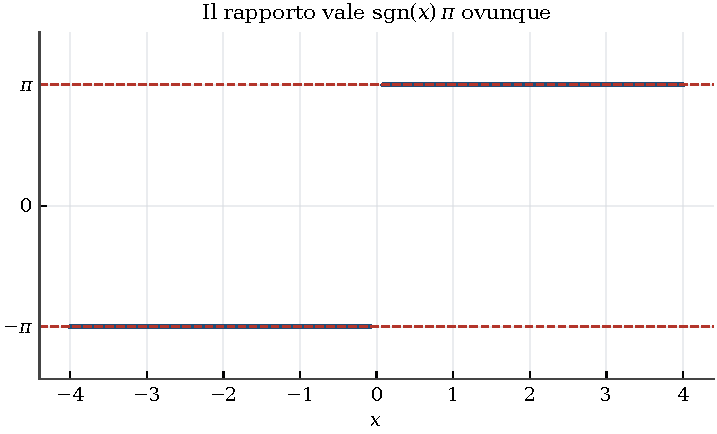
\includegraphics[width=0.86\linewidth]{../figures/pigreco_identita.pdf}
  \caption{Verifica numerica dell'identità $\#22$: il rapporto vale $\pi$ per $x>0$ e $-\pi$ per $x<0$, con le sole interruzioni nei punti in cui il denominatore si annulla.}
  \label{fig:pigreco_identita}
\end{figure}

L'identità è esatta e si dimostra in due mosse. La formula di duplicazione $\cos 2\theta=2\cos^2\theta-1$ trasforma il numeratore: $\cos 2x-\cos\tfrac2x=2\left(\cos^2 x-\cos^2\tfrac1x\right)$, e il rapporto con il denominatore vale dunque esattamente $2$, per ogni $x$ per cui il denominatore non si annulla. Resta il secondo fattore, $\arctan x+\arctan\tfrac1x$, che vale $\pi/2$ per $x>0$ e $-\pi/2$ per $x<0$: è l'identità classica dell'arcotangente del reciproco. Il prodotto è $2\cdot\mathrm{sgn}(x)\tfrac{\pi}{2}=\mathrm{sgn}(x)\,\pi$.

Detto altrimenti: il primo fattore è una costante travestita da funzione, il secondo è un gradino travestito da somma di arcotangenti, e il prodotto è un gradino di altezza $2\pi$. La riga $\#23$ riscrive la stessa cosa con gli sviluppi in serie di tutte le funzioni coinvolte, presumibilmente per verificare che l'identità non dipenda da proprietà nascoste delle funzioni chiuse.

\section{$\pi$ ed $\mathrm{e}$ come estremi di una stessa funzione}

L'ultimo episodio è il più breve.

\begin{espr}{24}{User}{}
\[
\left(\pi^{x} + \mathrm{e}^{x}\right)^{\frac{1}{x}}
\]
\end{espr}
La media di potenza di ordine $x$ fra $\pi$ ed $\mathrm{e}$.

\begin{espr}{25}{User}{\verificata}
\[
\lim_{x \to +\infty} \left(\pi^{x} + \mathrm{e}^{x}\right)^{\frac{1}{x}} = \pi
\]
\end{espr}
Per $x\to+\infty$ prevale la base maggiore.

\begin{espr}{26}{User}{\verificata}
\[
\lim_{x \to -\infty} \left(\pi^{x} + \mathrm{e}^{x}\right)^{\frac{1}{x}} = \mathrm{e}
\]
\end{espr}
Per $x\to-\infty$ prevale la minore. Una funzione, due costanti.


La funzione $\left(\pi^x+\mathrm{e}^x\right)^{1/x}$ è la media di potenza di ordine $x$ dei due numeri. Per $x\to+\infty$ il termine con la base maggiore domina e la media tende al massimo, cioè $\pi$; per $x\to-\infty$ domina il termine con la base minore e si ottiene $\mathrm{e}$. Una sola espressione contiene entrambe le costanti, ciascuna come limite da una parte. È lo stesso meccanismo per cui la norma $\ell^p$ di un vettore tende al massimo delle componenti quando $p$ diverge.

\section*{In sintesi}
\addcontentsline{toc}{section}{In sintesi}

Il quaderno raccoglie cinque strade indipendenti verso lo stesso numero: una derivazione ripetuta che lo lascia intatto, un prodotto che lo fa comparire in un fattore correttivo, un fattoriale semi-intero che lo produce esattamente, un rapporto trigonometrico che vale $\pi$ ovunque, e una media di potenze che lo raggiunge all'infinito. Solo la quarta è un'identità nel senso stretto — ed è anche l'unica che si dimostra in due righe.


%% generato automaticamente da tools/build_tex.py --- non modificare
\chapter{Le funzioni iperboliche di $\pi$ ed $\mathrm{e}$}
\label{cap:sin-cos}
\quaderno{sin-cos.dfw}{04 Jan 2010}{20}

Gennaio 2010. Venti espressioni che costruiscono, pezzo per pezzo, un sistema completo di funzioni iperboliche e circolari a partire da due sole basi: $\mathrm{e}^{\pi x}$ e $\pi^{\mathrm{e}x}$. È il quaderno tecnicamente più compatto della raccolta, perché tutto quello che contiene discende da una sola osservazione, che però non è mai scritta esplicitamente.

\section{Il sistema iperbolico}

L'osservazione da cui dipende tutto è questa: $\dfrac{\mathrm{e}^{\pi x}}{\pi^{\mathrm{e}x}}=\mathrm{e}^{\pi x-\mathrm{e}x\ln\pi}=\mathrm{e}^{kx}$, dove $k=\pi-\mathrm{e}\ln\pi$. Il rapporto fra le due potenze è dunque un semplice esponenziale, e la costante $k$ ne è la pulsazione. Da qui le prime quattro espressioni si leggono a colpo d'occhio.

\begin{espr}{1}{User}{}
\[
\frac{\frac{\mathrm{e}^{\pi\, x}}{\pi^{\mathrm{e}\, x}} + \frac{\pi^{\mathrm{e}\, x}}{\mathrm{e}^{\pi\, x}}}{2}
\]
\end{espr}
La semisomma del rapporto e del suo reciproco: è $\cosh(kx)$ con $k=\pi-\mathrm{e}\ln\pi$.

\begin{espr}{2}{User}{}
\[
\frac{\frac{\mathrm{e}^{\pi\, x}}{\pi^{\mathrm{e}\, x}} - \frac{\pi^{\mathrm{e}\, x}}{\mathrm{e}^{\pi\, x}}}{2}
\]
\end{espr}
La semidifferenza: $\sinh(kx)$.

\begin{espr}{3}{User}{}
\[
\frac{\mathrm{e}^{2\, \pi\, x} - \pi^{2\, \mathrm{e}\, x}}{\pi^{2\, \mathrm{e}\, x} + \mathrm{e}^{2\, \pi\, x}}
\]
\end{espr}
Il loro rapporto, cioè $\tanh(kx)$. Gli esponenti raddoppiati vengono dal prodotto delle due espressioni precedenti.

\begin{espr}{4}{User}{}
\[
\frac{\pi^{2\, \mathrm{e}\, x} + \mathrm{e}^{2\, \pi\, x}}{\mathrm{e}^{2\, \pi\, x} - \pi^{2\, \mathrm{e}\, x}}
\]
\end{espr}
Il reciproco: $\coth(kx)$.


Sono, nell'ordine, $\cosh(kx)$, $\sinh(kx)$, $\tanh(kx)$ e $\coth(kx)$. Le definizioni sono quelle canoniche — semisomma, semidifferenza, loro rapporto — solo scritte con basi inconsuete.

\section{Le derivate}

Le quattro espressioni successive sono le derivate delle precedenti, e confermano che il sistema è coerente: la costante $k$ compare come fattore, esattamente come ci si aspetta derivando una funzione di $kx$.

\begin{espr}{5}{User}{}
\[
\left(\pi - \mathrm{e}\, \ln\!\left(\pi\right)\right)\, \left(\frac{\frac{\mathrm{e}^{\pi\, x}}{\pi^{\mathrm{e}\, x}} - \frac{\pi^{\mathrm{e}\, x}}{\mathrm{e}^{\pi\, x}}}{2}\right)
\]
\end{espr}
$k\sinh(kx)$: la derivata del coseno iperbolico.

\begin{espr}{6}{User}{}
\[
\left(\pi - \mathrm{e}\, \ln\!\left(\pi\right)\right)\, \left(\frac{\frac{\mathrm{e}^{\pi\, x}}{\pi^{\mathrm{e}\, x}} + \frac{\pi^{\mathrm{e}\, x}}{\mathrm{e}^{\pi\, x}}}{2}\right)
\]
\end{espr}
$k\cosh(kx)$: la derivata del seno iperbolico.

\begin{espr}{7}{User}{}
\[
\frac{4\, \pi^{2\, \mathrm{e}\, x}\, \mathrm{e}^{2\, \pi\, x}\, \left(\pi - \mathrm{e}\, \ln\!\left(\pi\right)\right)}{\left(\mathrm{e}^{2\, \pi\, x} + \pi^{2\, \mathrm{e}\, x}\right)^{2}}
\]
\end{espr}
$k\,\mathrm{sech}^2(kx)$: la derivata della tangente iperbolica.

\begin{espr}{8}{User}{}
\[
\frac{4\, \pi^{2\, \mathrm{e}\, x}\, \mathrm{e}^{2\, \pi\, x}\, \left(\mathrm{e}\, \ln\!\left(\pi\right) - \pi\right)}{\left(\mathrm{e}^{2\, \pi\, x} - \pi^{2\, \mathrm{e}\, x}\right)^{2}}
\]
\end{espr}
$-k\,\mathrm{csch}^2(kx)$: la derivata della cotangente iperbolica. Il fattore $(\mathrm{e}\ln\pi-\pi)$ è $-k$.


In particolare $\#7$, che sembra un'espressione complicata, è $k\,\mathrm{sech}^2(kx)$: dividendo numeratore e denominatore per $\pi^{4\mathrm{e}x}$ resta $4k\,\mathrm{e}^{2kx}/\left(\mathrm{e}^{2kx}+1\right)^2$, che è la derivata della tangente iperbolica. L'espressione $\#8$ è invece $-k\,\mathrm{csch}^2(kx)$, la derivata della cotangente iperbolica.

\section{Il passaggio al caso circolare}

Sostituendo $x$ con $\mathrm{i}x$ le funzioni iperboliche diventano circolari. Le sei espressioni che seguono lo verificano e ne traggono la formula di addizione.

\begin{espr}{9}{User}{}
\begin{align*}
& \frac{\frac{\mathrm{e}^{\pi\, \left(\mathrm{i}\, x\right)}}{\pi^{\mathrm{e}\, \left(\mathrm{i}\, x\right)}} + \frac{\pi^{\mathrm{e}\, \left(\mathrm{i}\, x\right)}}{\mathrm{e}^{\pi\, \left(\mathrm{i}\, x\right)}}}{2} \\
=\;& \cos\!\left(\pi\, x\right)\, \cos\!\left(\mathrm{e}\, x\, \ln\!\left(\pi\right)\right) + \sin\!\left(\pi\, x\right)\, \sin\!\left(\mathrm{e}\, x\, \ln\!\left(\pi\right)\right) = \cos\!\left(\left(\pi - \mathrm{e}\, \ln\!\left(\pi\right)\right)\, x\right)
\end{align*}
\end{espr}
Sostituendo $x\to\mathrm{i}x$ il coseno iperbolico diventa circolare, e la scrittura esplicita è la formula di sottrazione del coseno.

\begin{espr}{10}{User}{\verificata}
\begin{align*}
& \frac{\frac{\mathrm{e}^{\pi\, \left(\mathrm{i}\, x\right)}}{\pi^{\mathrm{e}\, \left(\mathrm{i}\, x\right)}} - \frac{\pi^{\mathrm{e}\, \left(\mathrm{i}\, x\right)}}{\mathrm{e}^{\pi\, \left(\mathrm{i}\, x\right)}}}{2} \\
=\;& \mathrm{i}\, \left(\sin\!\left(\pi\, x\right)\, \cos\!\left(\mathrm{e}\, x\, \ln\!\left(\pi\right)\right) - \cos\!\left(\pi\, x\right)\, \sin\!\left(\mathrm{e}\, x\, \ln\!\left(\pi\right)\right)\right) \\
=\;& \mathrm{i}\, \sin\!\left(\left(\pi - \mathrm{e}\, \ln\!\left(\pi\right)\right)\, x\right)
\end{align*}
\end{espr}
Analogamente per il seno: il fattore $\mathrm{i}$ segnala che $\sinh(\mathrm{i}\theta)=\mathrm{i}\sin\theta$.

\begin{espr}{11}{User}{\verificata}
\begin{align*}
& \frac{\frac{\mathrm{e}^{\pi\, \left(\mathrm{i}\, x\right)}}{\pi^{\mathrm{e}\, \left(\mathrm{i}\, x\right)}} + \frac{\pi^{\mathrm{e}\, \left(\mathrm{i}\, x\right)}}{\mathrm{e}^{\pi\, \left(\mathrm{i}\, x\right)}}}{2} \\
&\qquad + \frac{\frac{\mathrm{e}^{\pi\, \left(\mathrm{i}\, x\right)}}{\pi^{\mathrm{e}\, \left(\mathrm{i}\, x\right)}} - \frac{\pi^{\mathrm{e}\, \left(\mathrm{i}\, x\right)}}{\mathrm{e}^{\pi\, \left(\mathrm{i}\, x\right)}}}{2} \\
=\;& \mathrm{e}^{\mathrm{i}\, x\, \left(\pi - \mathrm{e}\, \ln\!\left(\pi\right)\right)}
\end{align*}
\end{espr}
La somma delle due ricompone l'esponenziale complesso di pulsazione $k$.

\begin{espr}{12}{User}{\verificata}
\begin{align*}
& \frac{\frac{\mathrm{e}^{\pi\, \left(\mathrm{i}\, x\right)}}{\pi^{\mathrm{e}\, \left(\mathrm{i}\, x\right)}} + \frac{\pi^{\mathrm{e}\, \left(\mathrm{i}\, x\right)}}{\mathrm{e}^{\pi\, \left(\mathrm{i}\, x\right)}}}{2} \\
&\qquad - \frac{\frac{\mathrm{e}^{\pi\, \left(\mathrm{i}\, x\right)}}{\pi^{\mathrm{e}\, \left(\mathrm{i}\, x\right)}} - \frac{\pi^{\mathrm{e}\, \left(\mathrm{i}\, x\right)}}{\mathrm{e}^{\pi\, \left(\mathrm{i}\, x\right)}}}{2} \\
=\;& \mathrm{e}^{-\mathrm{i}\, x\, \left(\pi - \mathrm{e}\, \ln\!\left(\pi\right)\right)}
\end{align*}
\end{espr}
La differenza dà l'esponenziale coniugato.

\begin{espr}{13}{User}{\verificata}
\begin{align*}
& \frac{\frac{\mathrm{e}^{\pi\, \left(\mathrm{i}\, x\right)}}{\pi^{\mathrm{e}\, \left(\mathrm{i}\, x\right)}} + \frac{\pi^{\mathrm{e}\, \left(\mathrm{i}\, x\right)}}{\mathrm{e}^{\pi\, \left(\mathrm{i}\, x\right)}}}{2} \\
&\qquad + \frac{\mathrm{i}\, \left(\frac{\mathrm{e}^{\pi\, \left(\mathrm{i}\, x\right)}}{\pi^{\mathrm{e}\, \left(\mathrm{i}\, x\right)}} - \frac{\pi^{\mathrm{e}\, \left(\mathrm{i}\, x\right)}}{\mathrm{e}^{\pi\, \left(\mathrm{i}\, x\right)}}\right)}{2} \\
=\;& \cos\!\left(\left(\pi - \mathrm{e}\, \ln\!\left(\pi\right)\right)\, x\right) - \sin\!\left(\left(\pi - \mathrm{e}\, \ln\!\left(\pi\right)\right)\, x\right)
\end{align*}
\end{espr}
Una combinazione con il fattore $\mathrm{i}$: il risultato è $\cos-\sin$.

\begin{espr}{14}{User}{\verificata}
\begin{align*}
& \frac{\frac{\mathrm{e}^{\pi\, \left(\mathrm{i}\, x\right)}}{\pi^{\mathrm{e}\, \left(\mathrm{i}\, x\right)}} + \frac{\pi^{\mathrm{e}\, \left(\mathrm{i}\, x\right)}}{\mathrm{e}^{\pi\, \left(\mathrm{i}\, x\right)}}}{2} \\
&\qquad - \frac{\mathrm{i}\, \left(\frac{\mathrm{e}^{\pi\, \left(\mathrm{i}\, x\right)}}{\pi^{\mathrm{e}\, \left(\mathrm{i}\, x\right)}} - \frac{\pi^{\mathrm{e}\, \left(\mathrm{i}\, x\right)}}{\mathrm{e}^{\pi\, \left(\mathrm{i}\, x\right)}}\right)}{2} \\
=\;& \cos\!\left(\left(\pi - \mathrm{e}\, \ln\!\left(\pi\right)\right)\, x\right) + \sin\!\left(\left(\pi - \mathrm{e}\, \ln\!\left(\pi\right)\right)\, x\right)
\end{align*}
\end{espr}
L'altra combinazione: $\cos+\sin$.


La riga $\#9$ contiene la formula di sottrazione del coseno: $\cos(\pi x)\cos(\mathrm{e}x\ln\pi)+\sin(\pi x)\sin(\mathrm{e}x\ln\pi)=\cos\!\big((\pi-\mathrm{e}\ln\pi)x\big)$. Le due frequenze $\pi$ ed $\mathrm{e}\ln\pi$ sono quasi uguali, e la loro differenza è la piccolissima $k$: è il fenomeno del battimento, due oscillazioni rapide e vicine che si combinano in una lentissima. Le righe $\#11$ e $\#12$ ricompongono l'esponenziale complesso, e le ultime due danno le combinazioni $\cos\mp\sin$.

\section{Quanto vale $k$}

L'ultima sezione mette i numeri. Sono sei righe, e insieme dicono una cosa sola con precisione notevole.

\begin{espr}{15}{User}{\verificata}
\[
\pi - \mathrm{e}\, \ln\!\left(\pi\right) = 0.02989420638
\]
\end{espr}
Il valore numerico della costante: circa tre centesimi.

\begin{espr}{16}{User}{\verificata}
\[
\frac{\pi^{-\mathrm{e}}\, \mathrm{e}^{\pi}}{2} - \frac{\pi^{\mathrm{e}}\, \mathrm{e}^{-\pi}}{2} = 0.02989865914
\]
\end{espr}
Il seno iperbolico di $k$, calcolato dalla definizione. Notare che $\pi^{-\mathrm{e}}\mathrm{e}^{\pi}=\mathrm{e}^{k}$.

\begin{espr}{17}{User}{}
\begin{align*}
& \pi - \mathrm{e}\, \ln\!\left(\pi\right) \\
=\;& \frac{\frac{\mathrm{e}^{\pi\, x}}{\pi^{\mathrm{e}\, x}} - \frac{\pi^{\mathrm{e}\, x}}{\mathrm{e}^{\pi\, x}}}{2}
\end{align*}
\end{espr}
L'equazione $\sinh(kx)=k$: si chiede per quale $x$ il seno iperbolico restituisca l'argomento.

\begin{espr}{18}{User}{}
\begin{align*}
& x \\
=\;& \frac{\ln\!\left(\sqrt{\mathrm{e}^{2}\, \ln^{2}\!\left(\pi\right) - 2\, \pi\, \mathrm{e}\, \ln\!\left(\pi\right) + \pi^{2} + 1} - \mathrm{e}\, \ln\!\left(\pi\right) + \pi\right)}{\pi - \mathrm{e}\, \ln\!\left(\pi\right)} \\
=\;& 0.9998511159
\end{align*}
\end{espr}
La soluzione è $\operatorname{arcsinh}(k)/k$, cioè $0{,}99985$: non uno, e la distanza da uno misura la non linearità del seno iperbolico.

\begin{espr}{19}{User}{\verificata}
\[
\frac{\pi^{\mathrm{e}}\, \mathrm{e}^{-\pi}}{2} + \frac{\pi^{-\mathrm{e}}\, \mathrm{e}^{\pi}}{2} = 1.000446865
\]
\end{espr}
Il coseno iperbolico di $k$: eccede l'unità di circa $k^2/2=4{,}47\cdot10^{-4}$.

\begin{espr}{20}{User}{\verificata}
\begin{align*}
& \frac{\pi^{-\mathrm{e}}\, \mathrm{e}^{\pi}}{2} - \frac{\pi^{\mathrm{e}}\, \mathrm{e}^{-\pi}}{2} - \pi + \mathrm{e}\, \ln\!\left(\pi\right) \\
=\;& 4.452759521 \cdot 10^{-6}
\end{align*}
\end{espr}
Lo scarto $\sinh k-k$, che vale $k^3/6$. È il termine di terzo grado dello sviluppo in serie, isolato numericamente.

\begin{figure}[htbp]
  \centering
  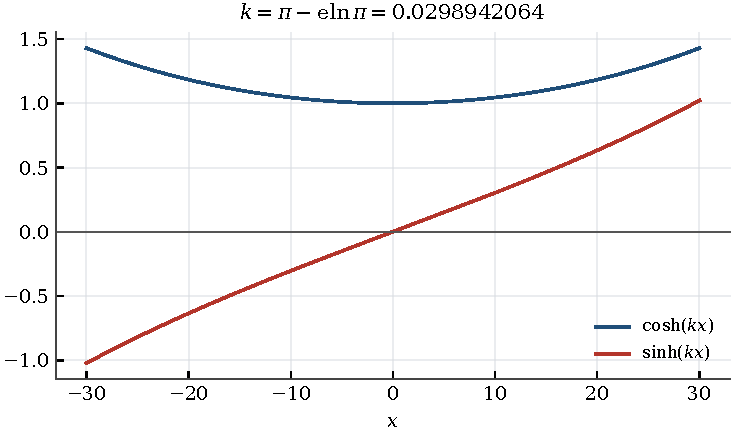
\includegraphics[width=0.86\linewidth]{../figures/sincos_pi_e.pdf}
  \caption{Le funzioni $\cosh(kx)$ e $\sinh(kx)$ costruite nel quaderno. La pulsazione $k=\pi-\mathrm{e}\ln\pi$ è così piccola che occorre arrivare a $|x|\approx 30$ per vederle crescere.}
  \label{fig:sincos_pi_e}
\end{figure}

Ecco il conto. La costante vale $k=\pi-\mathrm{e}\ln\pi=0{,}02989420\ldots$, un numero molto piccolo. La riga $\#16$ calcola $\sinh k=0{,}02989865\ldots$ e la riga $\#19$ calcola $\cosh k=1{,}000446865$. Per $k$ così piccolo si ha $\sinh k\approx k$ e $\cosh k\approx 1$, e le due righe lo confermano.

Ma il quaderno non si accontenta e chiede di quanto esattamente $\sinh k$ superi $k$: è la riga $\#20$, che dà $4{,}4527\cdot10^{-6}$. Questo numero è $k^3/6$, cioè il primo termine trascurato nello sviluppo $\sinh k=k+\tfrac{k^3}{3!}+\cdots$ — e infatti $0{,}0298942^3/6=4{,}4528\cdot10^{-6}$. Le sei righe finali sono, in sostanza, una verifica numerica dello sviluppo in serie del seno iperbolico, condotta su un argomento scelto in modo che il primo termine correttivo fosse misurabile.

La riga $\#18$ chiude con eleganza: risolvendo $\sinh(kx)=k$ si trova $x=\operatorname{arcsinh}(k)/k=0{,}9998511$. Il valore $x=1$ non è soluzione proprio perché $\sinh k\neq k$, e lo scarto dall'unità, un centocinquantamillesimo, è la misura di quella differenza.

\section*{In sintesi}
\addcontentsline{toc}{section}{In sintesi}

Il quaderno è costruito su una sola identità elementare — il rapporto fra $\mathrm{e}^{\pi x}$ e $\pi^{\mathrm{e}x}$ è $\mathrm{e}^{kx}$ — e su una sola osservazione numerica: quel $k$ è molto piccolo. Da lì discendono un sistema iperbolico completo con le sue derivate, il corrispondente sistema circolare, e una misura sperimentale del terzo termine dello sviluppo del seno iperbolico. Il numero $\sinh k=0{,}0298986\ldots$ che compare alla riga $\#16$ ricomparirà, sette mesi dopo, alla riga $\#69$ di \dfw{e.dfw} (capitolo~\ref{cap:e}), calcolato per un'altra strada e senza che il legame venga notato.


%% generato automaticamente da tools/build_tex.py --- non modificare
\chapter{Un nome per l'infinitesimo}
\label{cap:j}
\quaderno{j.dfw}{07 Jul 2009}{7}

Luglio 2009. Sette espressioni soltanto, ma è il quaderno che richiede più cautela nella lettura, perché due delle sue righe non vanno prese alla lettera. Il titolo del file — la lettera che gli ingegneri usano al posto di $\mathrm{i}$ — dice l'argomento: che cosa sia l'unità immaginaria, e se si possa raggiungerla per via di limiti.

\section{I due punti fissi dell'esponenziale complesso}

Le prime due righe sono la formula di Eulero valutata nei due punti in cui restituisce un numero reale.

\begin{espr}{1}{User}{\verificata}
\[
\cos\!\left(0\right) + \mathrm{i}\, \sin\!\left(0\right) = 1
\]
\end{espr}
La formula di Eulero in $x=0$.

\begin{espr}{2}{User}{\verificata}
\[
\cos\!\left(\pi\right) + \mathrm{i}\, \sin\!\left(\pi\right) = -1
\]
\end{espr}
E in $x=\pi$: è l'identità di Eulero nella forma $\mathrm{e}^{\mathrm{i}\pi}+1=0$.

\section{Due limiti e un nome}

Le due righe successive sono il cuore del quaderno e vanno lette con attenzione, perché così come sono scritte non sono vere nel senso ordinario.

\begin{espr}{3}{User}{}
\[
\mathrm{i} = \lim_{x \to 0} \frac{1 - \cos\!\left(x\right)}{\sin\!\left(x\right)}
\]
\end{espr}
Il rapporto vale $\tan(x/2)$ e il suo limite in zero è zero. L'identificazione con $\mathrm{i}$ è una convenzione di scrittura, non un'uguaglianza numerica.

\begin{espr}{4}{User}{}
\[
-\mathrm{i} = \lim_{x \to \pi} \frac{1 + \cos\!\left(x\right)}{\sin\!\left(x\right)}
\]
\end{espr}
Il rapporto vale $\cot(x/2)$ e il suo limite in $\pi$ è zero, per la stessa ragione e con segno convenzionalmente opposto.

\begin{figure}[htbp]
  \centering
  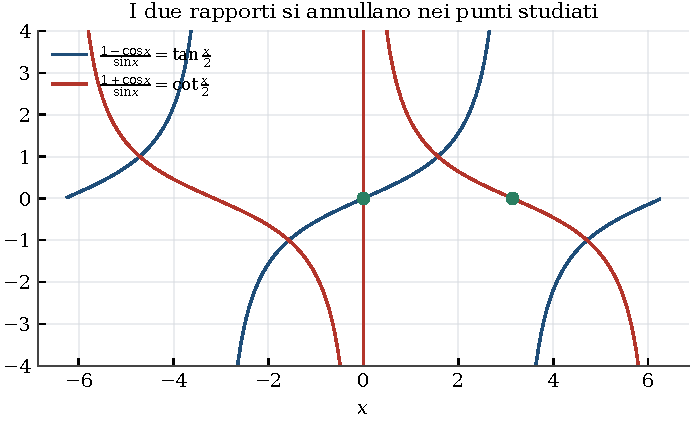
\includegraphics[width=0.86\linewidth]{../figures/j_tan.pdf}
  \caption{I due rapporti delle righe $\#3$ e $\#4$ coincidono con $\tan(x/2)$ e $\cot(x/2)$. I cerchi segnano i punti in cui vengono valutati i limiti: in entrambi il valore è zero.}
  \label{fig:j_tan}
\end{figure}

Entrambe le espressioni a secondo membro si semplificano con le formule di bisezione:
\[
  \frac{1-\cos x}{\sin x}=\tan\frac{x}{2},
  \qquad
  \frac{1+\cos x}{\sin x}=\cot\frac{x}{2}.
\]
Il primo tende a $\tan 0=0$ per $x\to0$; il secondo tende a $\cot(\pi/2)=0$ per $x\to\pi$. Nel senso ordinario dell'analisi entrambi i limiti valgono zero, e Derive stesso risponde zero se glielo si chiede.

Che cosa intendeva allora l'autore scrivendo $\mathrm{i}$ e $-\mathrm{i}$? La lettura più coerente con il resto della raccolta è che si tratti di un battesimo, non di un'uguaglianza: alle due quantità infinitesime prodotte dai due limiti viene dato un nome, esattamente come nel quaderno del maggio precedente si dava il nome $\varepsilon$ al difetto di un'operazione (capitolo~\ref{cap:teoria}). Il segno opposto distingue i due lati.

C'è però anche una lettura più tecnica, e vale la pena di indicarla. La quantità $\tan(x/2)$ è il parametro della sostituzione di Weierstrass, quella che parametrizza razionalmente il cerchio unitario e che ricomparirà in \dfw{gauss.dfw} e in \dfw{delta.dfw} nella forma $\mathrm{e}^{\mathrm{i}x}=\big(1+\mathrm{i}\tan\tfrac{x}{2}\big)^2\big/\big(1+\tan^2\tfrac{x}{2}\big)$. In quella parametrizzazione $x=0$ e $x=\pi$ sono precisamente i due punti in cui l'esponenziale vale $+1$ e $-1$: le righe $\#3$ e $\#4$ marcano quei due punti, che sono gli stessi delle righe $\#1$ e $\#2$.

\section{Che cosa succede elevando a potenza}

Le ultime tre righe mettono alla prova l'oggetto appena battezzato: che cosa gli accade se lo si eleva a una potenza che cresce?

\begin{espr}{5}{User}{\verificata}
\[
\cos\!\left(x\right) + \mathrm{i}\, \sin\!\left(x\right) = \mathrm{e}^{\mathrm{i}\, x}
\]
\end{espr}
La formula di Eulero in forma generale: la riga che dà senso alle due precedenti.

\begin{espr}{6}{User}{}
\[
\lim_{n \to +\infty} \left(\lim_{x \to 0} \frac{1 - \cos\!\left(x\right)}{\sin\!\left(x\right)}\right)^{n}
\]
\end{espr}
L'oggetto battezzato, elevato a una potenza che tende all'infinito.

\begin{espr}{7}{User}{}
\[
\left(\frac{1 - \cos\!\left(10^{-x}\right)}{\sin\!\left(10^{-x}\right)}\right)^{x}
\]
\end{espr}
La versione calcolabile: argomento $10^{-x}$ ed esponente $x$. La quantità decresce come $10^{-x^2}$.


La riga $\#7$ è la versione concreta e calcolabile della domanda: si prende l'argomento $x=10^{-n}$, cioè lo si fa tendere a zero per potenze di dieci, e si eleva alla $n$. Poiché $\tan(10^{-n}/2)\approx 10^{-n}/2$, la quantità vale circa $10^{-n^2}2^{-n}$: non tende a zero come una potenza, ma come una gaussiana negli esponenti. Se l'oggetto fosse davvero $\mathrm{i}$, il suo modulo resterebbe $1$ per sempre; il fatto che collassi così rapidamente è la prova che infinitesimo e unità immaginaria non sono la stessa cosa. Il quaderno, che è del 2009, non torna sull'argomento.

\section*{In sintesi}
\addcontentsline{toc}{section}{In sintesi}

Sette righe che pongono una domanda legittima — l'unità immaginaria si può ottenere come limite di quantità reali? — e le danno una risposta implicita ma netta. No, e la riga $\#7$ mostra perché: ciò che quei limiti producono ha modulo che tende a zero, mentre $\mathrm{i}$ ha modulo uno. La risposta affermativa arriverà, ma da un'altra strada: nel quaderno \dfw{e.dfw} dell'agosto 2010 (capitolo~\ref{cap:e}, righe $\#88$--$\#92$), dove $\mathrm{i}$ si ottiene come limite di $\left(1+\tfrac{\mathrm{i}\pi}{2x}\right)^x$ — cioè lasciando l'unità immaginaria nella formula fin dall'inizio.


%% generato automaticamente da tools/build_tex.py --- non modificare
\chapter{L'arcotangente attraversa il taglio}
\label{cap:atan}
\quaderno{atan.dfw}{28 Jan 2010}{14}

Gennaio 2010. Quattordici espressioni che partono da un'identità nota e la seguono fuori dal territorio in cui è nata. L'identità è che $\mathrm{e}^{\mathrm{i}\arctan x}$ è il numero complesso $1+\mathrm{i}x$ normalizzato; la domanda del quaderno è che cosa ne resti quando all'argomento reale si sostituisce un argomento immaginario. La risposta passa per il punto di diramazione dell'arcotangente e per il logaritmo complesso.

\section{Il punto di partenza}

La prima riga contiene tre scritture della stessa cosa, ed è l'osservazione su cui poggia tutto il resto: l'arcotangente di $x$ è l'argomento del numero complesso $1+\mathrm{i}x$.

\begin{espr}{1}{User}{}
\[
\mathrm{e}^{\mathrm{i}\, \arctan\!\left(x\right)} = \frac{1 + \mathrm{i}\, x}{\sqrt{x^{2} + 1}} = \operatorname{sgn}\!\left(1 + \mathrm{i}\, x\right)
\]
\end{espr}
Tre scritture equivalenti. L'identità è esatta per ogni $x$ reale; il verificatore automatico non le assegna il segno di spunta perché lo prova su punti complessi, dove l'arcotangente cambia ramo.

\begin{figure}[htbp]
  \centering
  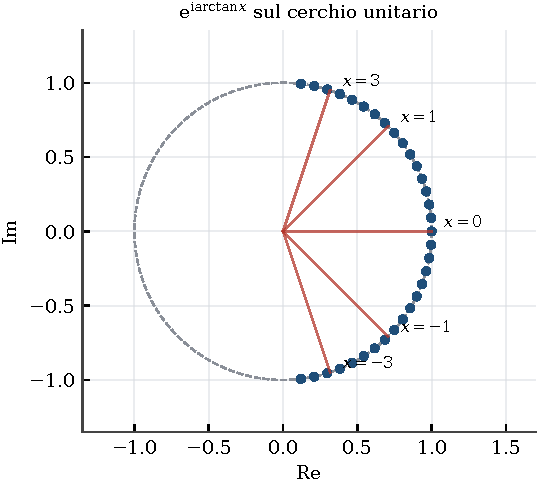
\includegraphics[width=0.58\linewidth]{../figures/atan_cerchio.pdf}
  \caption{L'identità $\#1$ in figura: al variare di $x$ reale il punto $(1+\mathrm{i}x)/\sqrt{1+x^2}$ percorre il semicerchio destro, e il suo argomento è $\arctan x$. Gli estremi $x\to\pm\infty$ corrispondono ai due punti $\pm\mathrm{i}$, che non vengono mai raggiunti.}
  \label{fig:atan_cerchio}
\end{figure}
\begin{espr}{2}{User}{\verificata}
\[
\mathrm{e}^{\mathrm{i}\, \arctan\!\left(\mathrm{i}\, x\right)} = \frac{1 - x}{\sqrt{1 - x^{2}}}
\]
\end{espr}
La sostituzione $x\to\mathrm{i}x$. Il secondo membro è $\sqrt{(1-x)/(1+x)}$ scritto senza radice al numeratore.


L'ultima delle tre scritture usa la funzione segno nel senso in cui Derive la estende ai complessi: $\mathrm{sgn}(z)=z/|z|$, cioè la proiezione sul cerchio unitario. Dire che $\mathrm{e}^{\mathrm{i}\arctan x}=\mathrm{sgn}(1+\mathrm{i}x)$ è dire che l'esponenziale immaginario è la fase, e nient'altro.

La riga $\#2$ compie il passo decisivo sostituendo $x\to\mathrm{i}x$. Poiché $\arctan(\mathrm{i}x)=\mathrm{i}\,\mathrm{artanh}(x)$, il primo membro diventa $\mathrm{e}^{-\mathrm{artanh}(x)}=\sqrt{\frac{1-x}{1+x}}$, che è esattamente il secondo membro riscritto. L'esponenziale immaginario è diventato un esponenziale reale: la rotazione si è trasformata in una dilatazione.

\section{Il punto di diramazione}

Che cosa succede esattamente in $x=1$, cioè quando l'argomento immaginario raggiunge $\mathrm{i}$?

\begin{espr}{3}{User}{}
\[
\arctan\!\left(\mathrm{i}\right) = \mathrm{i}\, \infty
\]
\end{espr}
Il punto di diramazione dell'arcotangente. La notazione $\mathrm{i}\infty$ indica una divergenza lungo l'asse immaginario.

\begin{espr}{4}{User}{}
\[
\mathrm{e}^{\mathrm{i}\, \arctan\!\left(\mathrm{i}\right)} = 0
\]
\end{espr}
Di conseguenza l'esponenziale si annulla: $\mathrm{e}^{-\infty}=0$.


L'arcotangente ha due punti di diramazione, in $\pm\mathrm{i}$, e lì diverge. Derive lo dice nel modo più diretto possibile: $\arctan(\mathrm{i})=\mathrm{i}\infty$. L'esponenziale corrispondente, avendo esponente reale negativo infinito, vale zero. È il collasso del cerchio unitario in un punto.

\section{La forma logaritmica e il ramo principale}

Le sei espressioni seguenti sviluppano l'arcotangente immaginaria in forma logaritmica e ne seguono le conseguenze passo per passo. È la parte più delicata del quaderno, perché è dove i rami del logaritmo entrano in gioco.

\begin{espr}{5}{User}{\verificata}
\[
\arctan\!\left(\mathrm{i}\, x\right) = -\frac{\pi}{2} + \frac{\mathrm{i}}{2}\, \left(\ln\!\left(x + 1\right) - \ln\!\left(x - 1\right)\right)
\]
\end{espr}
Lo sviluppo logaritmico dell'arcotangente immaginaria, nella forma valida per $x>1$. Il termine $-\pi/2$ è il contributo del ramo principale.

\begin{espr}{6}{User}{\verificata}
\begin{align*}
& \mathrm{i}\, \arctan\!\left(\mathrm{i}\, x\right) \\
=\;& -\frac{1}{2}\, \left(\ln\!\left(x + 1\right) - \ln\!\left(x - 1\right)\right) - \frac{\mathrm{i}\, \pi}{2}
\end{align*}
\end{espr}
Moltiplicata per $\mathrm{i}$: la parte immaginaria e quella reale si scambiano di ruolo.

\begin{espr}{7}{User}{\verificata}
\begin{align*}
& \mathrm{e}^{\mathrm{i}\, \arctan\!\left(\mathrm{i}\, x\right)} \\
=\;& \mathrm{e}^{-\frac{1}{2}\, \left(\ln\!\left(x + 1\right) - \ln\!\left(x - 1\right)\right) - \frac{\mathrm{i}\, \pi}{2}}
\end{align*}
\end{espr}
L'esponenziale della riga precedente.

\begin{espr}{8}{User}{\verificata}
\begin{align*}
& \mathrm{e}^{-\frac{1}{2}\, \left(\ln\!\left(x + 1\right) - \ln\!\left(x - 1\right)\right)}\, \mathrm{e}^{\frac{-\mathrm{i}\, \pi}{2}} \\
=\;& -\mathrm{i}\, \mathrm{e}^{-\frac{1}{2}\, \left(\ln\!\left(x + 1\right) - \ln\!\left(x - 1\right)\right)}
\end{align*}
\end{espr}
Il fattore $\mathrm{e}^{-\mathrm{i}\pi/2}$ vale $-\mathrm{i}$ e viene portato fuori.

\begin{espr}{9}{User}{\verificata}
\[
\mathrm{e}^{-\frac{1}{2}\, \left(\ln\!\left(x + 1\right) - \ln\!\left(x - 1\right)\right)} = \frac{\sqrt{x - 1}}{\sqrt{x + 1}}
\]
\end{espr}
Il fattore restante si semplifica in una radice: $\mathrm{e}^{-\frac12\ln\frac{x+1}{x-1}}=\sqrt{\frac{x-1}{x+1}}$.

\begin{espr}{10}{User}{\verificata}
\[
\mathrm{e}^{\mathrm{i}\, \arctan\!\left(\mathrm{i}\, x\right)} = \frac{1}{\mathrm{i}}\, \left(\frac{\sqrt{x - 1}}{\sqrt{x + 1}}\right)
\]
\end{espr}
Mettendo insieme: l'esponenziale vale la radice divisa per $\mathrm{i}$.


La riga $\#5$ merita un commento. La formula scolastica sarebbe $\arctan(\mathrm{i}x)=\tfrac{\mathrm{i}}{2}\ln\frac{1+x}{1-x}$, valida per $|x|<1$. Quella scritta qui usa invece $\ln(x-1)$ al posto di $\ln(1-x)$, e compensa con il termine costante $-\pi/2$. Non è un errore: è la continuazione analitica oltre il punto di diramazione, cioè la forma valida per $x>1$, dove $\ln(x-1)$ è reale e la scelta del ramo principale di Derive — dichiarata nell'intestazione del file con $\mathtt{Branch{:}{=}Principal}$ — aggiunge quel $-\pi/2$. Le righe successive riducono l'esponenziale a $\sqrt{(x-1)/(x+1)}$ diviso per $\mathrm{i}$, che è la controparte per $x>1$ della radice $\sqrt{(1-x)/(1+x)}$ trovata alla riga $\#2$ per $|x|<1$.

\section{La verifica per via inversa}

Le ultime quattro righe rifanno il conto al contrario: invece di sviluppare l'arcotangente, si pone l'esponenziale uguale al risultato e si risolve per l'esponente.

\begin{espr}{11}{User}{}
\[
\mathrm{e}^{z} = \frac{1 - x}{\sqrt{1 - x^{2}}}
\]
\end{espr}
Si riparte dal risultato della riga $\#2$ e lo si pone uguale a $\mathrm{e}^z$, per ricavare $z$.

\begin{espr}{12}{Simp(Solve(\#11,z))}{}
\begin{align*}
& z = -\frac{\ln\!\left(1 - x^{2}\right)}{2} + \ln\!\left(1 - x\right) - 2\, \pi\, \mathrm{i} \\[3pt]
\lor\quad & z = -\frac{\ln\!\left(1 - x^{2}\right)}{2} + \ln\!\left(1 - x\right) + 2\, \pi\, \mathrm{i} \\[3pt]
\lor\quad & z = \ln\!\left(1 - x\right) - \frac{\ln\!\left(1 - x^{2}\right)}{2}
\end{align*}
\end{espr}
Le tre soluzioni di Derive differiscono per multipli di $2\pi\mathrm{i}$: sono rami distinti dello stesso logaritmo.

\begin{espr}{13}{User}{}
\[
z = \ln\!\left(1 - x\right) - \frac{\ln\!\left(1 - x^{2}\right)}{2}
\]
\end{espr}
Il ramo principale, quello senza termine immaginario aggiunto.

\begin{espr}{14}{User}{\verificata}
\[
\mathrm{i}\, \arctan\!\left(\mathrm{i}\, x\right) = \ln\!\left(1 - x\right) - \frac{\ln\!\left(1 - x^{2}\right)}{2}
\]
\end{espr}
La conclusione: $\mathrm{i}\arctan(\mathrm{i}x)=\ln(1-x)-\tfrac12\ln(1-x^2)$, che è $-\mathrm{artanh}(x)$ scritto per esteso.


Fra le tre soluzioni che Derive restituisce alla riga $\#12$, due differiscono dalla terza per multipli di $2\pi\mathrm{i}$: sono i rami del logaritmo complesso, che il programma elenca tutti perché nessuno è privilegiato dall'equazione. La riga $\#13$ sceglie quello principale e la riga $\#14$ conclude, chiudendo il cerchio con la riga $\#2$.

\section*{In sintesi}
\addcontentsline{toc}{section}{In sintesi}

Il quaderno segue una funzione elementare fuori dal suo dominio naturale e registra con precisione che cosa le accade: l'esponenziale immaginario diventa reale, il cerchio unitario si apre in una semiretta, e in $x=1$ tutto collassa in un punto. Le righe da $\#5$ a $\#10$ sono un esercizio di contabilità dei rami del logaritmo condotto senza errori, il che con un sistema di calcolo simbolico non è mai scontato. Visto dall'altro lato, il risultato è la formula $\mathrm{e}^{s}=\left(1+\tanh\tfrac s2\right)/\left(1-\tanh\tfrac s2\right)$: la stessa tangente del semiangolo che in \dfw{gauss.dfw} produce la gaussiana, come mostra la nota a corredo di questa edizione.


%% generato automaticamente da tools/build_tex.py --- non modificare
\chapter{Equazioni algebriche spezzate in due}
\label{cap:equazioni}
\quaderno{equazioni.dfw}{27 Jan 2010}{44}

Gennaio 2010. Il quaderno applica una sola idea a quattro casi, di grado crescente dal primo al quarto. L'idea è questa: invece di risolvere un'equazione algebrica nel campo complesso, si scrive l'incognita come $z=x+\mathrm{i}y$ con $x$ e $y$ reali, si separano parte reale e parte immaginaria, e si ottiene un sistema di due equazioni reali in due incognite. È il metodo che, in geometria, corrisponde a cercare le radici come intersezioni di due curve nel piano.

\section{Primo grado}

Il caso più semplice serve a fissare la procedura. Il risultato è noto, ma il modo in cui si arriva merita di essere visto perché è quello che verrà ripetuto tre volte.

\begin{espr}{1}{User}{}
\[
a\, z + b = 0
\]
\end{espr}
L'equazione di primo grado nel campo complesso.

\begin{espr}{2}{User}{}
\[
z = x + \mathrm{i}\, y
\]
\end{espr}
La sostituzione che genera tutto il resto.

\begin{espr}{3}{Sub(\#1)}{}
\[
a\, \left(x + \mathrm{i}\, y\right) + b = 0
\]
\end{espr}
Sostituita.

\begin{espr}{4}{User}{}
\[
a\, x + b + \mathrm{i}\, a\, y = 0
\]
\end{espr}
Sviluppata, con parte reale e immaginaria separate.

\begin{espr}{5}{User}{}
\[
\operatorname{Re}\!\left(a\, x + b + \mathrm{i}\, a\, y\right) = 0
\]
\end{espr}
La condizione sulla parte reale.

\begin{espr}{6}{User}{}
\[
\operatorname{Im}\!\left(a\, x + b + \mathrm{i}\, a\, y\right) = 0
\]
\end{espr}
E quella sulla parte immaginaria.

\begin{espr}{7}{User}{}
\[
z = -\frac{b}{a} + \mathrm{i}\, 0
\]
\end{espr}
La soluzione, scritta con la parte immaginaria esplicitamente nulla.


La parte immaginaria dà $ay=0$, cioè $y=0$: l'equazione di primo grado a coefficienti reali non ha radici fuori dall'asse reale. La parte reale dà allora $x=-b/a$. La riga $\#7$ scrive la soluzione nella forma completa $z=-b/a+\mathrm{i}\cdot0$, che sembra pedante ma è il punto: il metodo restituisce sempre una coppia, ed è la coppia a dire dove si trova la radice.

\section{Secondo grado}

Qui il metodo comincia a dare qualcosa in cambio. Sostituendo $z=x+\mathrm{i}y$ nella forma generale e separando, si ottengono due coniche.

\begin{espr}{8}{User}{}
\[
a\, z^{2} + b\, z + c = 0
\]
\end{espr}
L'equazione di secondo grado.

\begin{espr}{9}{User}{}
\[
z = x + \mathrm{i}\, y
\]
\end{espr}
La stessa sostituzione.

\begin{espr}{10}{User}{}
\[
a\, x^{2} + b\, x - a\, y^{2} + c + \mathrm{i}\, \left(2\, a\, x\, y + b\, y\right) = 0
\]
\end{espr}
Lo sviluppo. La parte immaginaria è già raccolta a fattor comune per $y$.

\begin{espr}{11}{User}{}
\[
\operatorname{Re}\!\left(a\, x^{2} + b\, x - a\, y^{2} + c + \mathrm{i}\, \left(2\, a\, x\, y + b\, y\right)\right) = 0
\]
\end{espr}
La condizione sulla parte reale: un'iperbole equilatera nel piano $(x,y)$.

\begin{espr}{12}{User}{}
\[
\operatorname{Im}\!\left(a\, x^{2} + b\, x - a\, y^{2} + c + \mathrm{i}\, \left(2\, a\, x\, y + b\, y\right)\right) = 0
\]
\end{espr}
La condizione sulla parte immaginaria.

\begin{espr}{13}{Simp(\#11)}{}
\[
a\, x^{2} + b\, x - a\, y^{2} + c = 0
\]
\end{espr}
Semplificata.

\begin{espr}{14}{Simp(\#12)}{}
\[
2\, a\, x\, y + b\, y = 0
\]
\end{espr}
Semplificata: il prodotto $y(2ax+b)$ deve annullarsi.

\begin{espr}{15}{Simp(User)}{}
\[
\left[\, x = -\frac{b}{2\, a} \;\land\; y = \frac{\sqrt{4\, a\, c - b^{2}}}{2\, \left|a\right|},\; x = -\frac{b}{2\, a} \;\land\; y = -\frac{\sqrt{4\, a\, c - b^{2}}}{2\, \left|a\right|},\; x = -\frac{\sqrt{b^{2} - 4\, a\, c} + b}{2\, a} \;\land\; y = 0,\; x = \frac{\sqrt{b^{2} - 4\, a\, c} - b}{2\, a} \;\land\; y = 0 \,\right]
\]
\end{espr}
I quattro casi. I primi due sono la coppia coniugata quando $4ac>b^2$, gli altri due le radici reali quando $b^2>4ac$.

\begin{figure}[htbp]
  \centering
  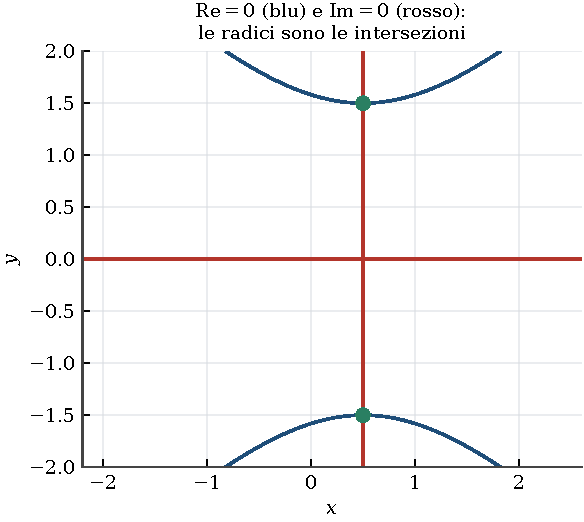
\includegraphics[width=0.62\linewidth]{../figures/equazioni_reim.pdf}
  \caption{Il metodo in figura, per $z^2-z+2{,}5=0$. La curva blu è il luogo $\operatorname{Re}=0$, la rossa il luogo $\operatorname{Im}=0$; quest'ultima è l'unione dell'asse reale e della verticale $x=-b/(2a)$, come impone la fattorizzazione. Le radici sono le intersezioni.}
  \label{fig:equazioni_reim}
\end{figure}

La parte immaginaria è $y(2ax+b)=0$, e questa fattorizzazione è tutto. O si annulla $y$ — e allora la radice è reale — oppure si annulla il secondo fattore, e allora $x=-b/(2a)$: le radici complesse stanno necessariamente sulla verticale per il vertice della parabola.

La riga $\#15$ elenca i quattro casi che ne derivano, e sono esattamente i due regimi della formula risolutiva. Se $4ac>b^2$ si hanno due radici coniugate con $x=-b/(2a)$ e $y=\pm\sqrt{4ac-b^2}/(2|a|)$; se $b^2>4ac$ si hanno due radici reali con $y=0$. Il discriminante non compare mai come tale: emerge da solo come condizione di realtà di una radice quadrata.

\section{Terzo grado}

Il grado tre è dove il metodo mostra la sua natura geometrica. La parte immaginaria continua a fattorizzarsi con $y$ in evidenza, ma il secondo fattore è ora una conica in $x$ e $y$.

\begin{espr}{16}{User}{}
\[
a\, z^{3} + b\, z^{2} + c\, z + d = 0
\]
\end{espr}
Si passa al terzo grado.

\begin{espr}{17}{User}{}
\[
z = x + \mathrm{i}\, y
\]
\end{espr}
Sostituzione.

\begin{espr}{18}{Sub(\#16)}{}
\[
a\, \left(x + \mathrm{i}\, y\right)^{3} + b\, \left(x + \mathrm{i}\, y\right)^{2} + c\, \left(x + \mathrm{i}\, y\right) + d = 0
\]
\end{espr}
Sostituita, senza sviluppare.

\begin{espr}{19}{User}{}
\begin{align*}
& a\, x^{3} + b\, x^{2} + x\, \left(c - 3\, a\, y^{2}\right) - b\, y^{2} + d + \mathrm{i}\, y\, \left(3\, a\, x^{2} + 2\, b\, x - a\, y^{2} + c\right) \\
=\;& 0
\end{align*}
\end{espr}
Sviluppata: la parte immaginaria è ancora un multiplo di $y$.

\begin{espr}{20}{User}{}
\begin{align*}
& \operatorname{Re}\!\left(a\, x^{3} + b\, x^{2} + x\, \left(c - 3\, a\, y^{2}\right) - b\, y^{2} + d + \mathrm{i}\, y\, \left(3\, a\, x^{2} + 2\, b\, x - a\, y^{2} + c\right)\right) \\
=\;& 0
\end{align*}
\end{espr}
Condizione sulla parte reale.

\begin{espr}{21}{User}{}
\begin{align*}
& \operatorname{Im}\!\left(a\, x^{3} + b\, x^{2} + x\, \left(c - 3\, a\, y^{2}\right) - b\, y^{2} + d + \mathrm{i}\, y\, \left(3\, a\, x^{2} + 2\, b\, x - a\, y^{2} + c\right)\right) \\
=\;& 0
\end{align*}
\end{espr}
E sulla parte immaginaria.

\begin{espr}{22}{Simp(\#20)}{}
\[
a\, x^{3} + b\, x^{2} + x\, \left(c - 3\, a\, y^{2}\right) - b\, y^{2} + d = 0
\]
\end{espr}
La cubica in $x$ con i termini in $y^2$.

\begin{espr}{23}{Simp(\#21)}{}
\[
y\, \left(3\, a\, x^{2} + 2\, b\, x - a\, y^{2} + c\right) = 0
\]
\end{espr}
Il prodotto che deve annullarsi. Il secondo fattore contiene la derivata della cubica.

\begin{espr}{24}{User}{}
\[
3\, a\, x^{2} + 2\, b\, x - a\, y^{2} + c = 0
\]
\end{espr}
Il secondo fattore isolato: una conica.

\begin{espr}{25}{Simp(Solve(\#24,y))}{}
\[
y = -\sqrt{\frac{3\, a\, x^{2} + 2\, b\, x + c}{a}} \;\lor\; y = \sqrt{\frac{3\, a\, x^{2} + 2\, b\, x + c}{a}}
\]
\end{espr}
Risolta rispetto a $y$: due rami simmetrici.

\begin{espr}{26}{User}{}
\[
y = 0
\]
\end{espr}
L'altro ramo della dicotomia.

\begin{espr}{27}{Sub(\#22)}{}
\begin{align*}
& a\, x^{3} + b\, x^{2} + x\, \left(c - 3\, a\, \left(-\sqrt{\frac{3\, a\, x^{2} + 2\, b\, x + c}{a}}\right)^{2}\right) - b\, \left(-\sqrt{\frac{3\, a\, x^{2} + 2\, b\, x + c}{a}}\right)^{2} \\
&\qquad + d \\
=\;& 0
\end{align*}
\end{espr}
Si sostituisce il valore di $y$ nella parte reale.

\begin{espr}{28}{Simp(\#27)}{}
\[
-\frac{8\, a^{2}\, x^{3} + 8\, a\, b\, x^{2} + 2\, x\, \left(a\, c + b^{2}\right) - a\, d + b\, c}{a} = 0
\]
\end{espr}
Il risultato: una cubica nella sola $x$, che dà l'ascissa della coppia coniugata.

\begin{espr}{29}{Simp(Solve(\#28,x))}{}
\begin{align*}
& x = \frac{-\sqrt{b^{2} - 3\, a\, c}\, \cos\!\left(\frac{\arccos\!\left(\frac{-\left(27\, a^{2}\, d - 9\, a\, b\, c + 2\, b^{3}\right)\, \operatorname{sgn}\!\left(a\right)}{2\, \left(b^{2} - 3\, a\, c\right)^{\frac{3}{2}}}\right)}{3}\right)}{3\, \left|a\right|} - \frac{b}{3\, a} \\[3pt]
\lor\quad & x = \frac{\sqrt{b^{2} - 3\, a\, c}\, \sin\!\left(\frac{\arcsin\!\left(\frac{\left(27\, a^{2}\, d - 9\, a\, b\, c + 2\, b^{3}\right)\, \operatorname{sgn}\!\left(a\right)}{2\, \left(b^{2} - 3\, a\, c\right)^{\frac{3}{2}}}\right)}{3} + \frac{\pi}{3}\right)}{3\, \left|a\right|} - \frac{b}{3\, a} \\[3pt]
\lor\quad & x = \frac{-\sqrt{b^{2} - 3\, a\, c}\, \sin\!\left(\frac{\arcsin\!\left(\frac{\left(27\, a^{2}\, d - 9\, a\, b\, c + 2\, b^{3}\right)\, \operatorname{sgn}\!\left(a\right)}{2\, \left(b^{2} - 3\, a\, c\right)^{\frac{3}{2}}}\right)}{3}\right)}{3\, \left|a\right|} - \frac{b}{3\, a}
\end{align*}
\end{espr}
\begin{espr}{30}{User}{}
\[
y = -\sqrt{\frac{3\, a\, x^{2} + 2\, b\, x + c}{a}} \;\lor\; y = \sqrt{\frac{3\, a\, x^{2} + 2\, b\, x + c}{a}}
\]
\end{espr}
I due rami, riscritti.

\begin{espr}{31}{Simp(Sub(\#22))}{}
\[
a\, x^{3} + b\, x^{2} + c\, x + d = 0
\]
\end{espr}
Sostituendo invece $y=0$ si ritrova l'equazione di partenza: il ramo delle radici reali.

\begin{espr}{32}{Simp(Solve(\#31,x))}{}
\begin{align*}
& x = \frac{2\, \sqrt{b^{2} - 3\, a\, c}\, \cos\!\left(\frac{\arccos\!\left(\frac{-\left(27\, a^{2}\, d - 9\, a\, b\, c + 2\, b^{3}\right)\, \operatorname{sgn}\!\left(a\right)}{2\, \left(b^{2} - 3\, a\, c\right)^{\frac{3}{2}}}\right)}{3}\right)}{3\, \left|a\right|} - \frac{b}{3\, a} \\[3pt]
\lor\quad & x = \frac{-2\, \sqrt{b^{2} - 3\, a\, c}\, \sin\!\left(\frac{\arcsin\!\left(\frac{\left(27\, a^{2}\, d - 9\, a\, b\, c + 2\, b^{3}\right)\, \operatorname{sgn}\!\left(a\right)}{2\, \left(b^{2} - 3\, a\, c\right)^{\frac{3}{2}}}\right)}{3} + \frac{\pi}{3}\right)}{3\, \left|a\right|} - \frac{b}{3\, a} \\[3pt]
\lor\quad & x = \frac{2\, \sqrt{b^{2} - 3\, a\, c}\, \sin\!\left(\frac{\arcsin\!\left(\frac{\left(27\, a^{2}\, d - 9\, a\, b\, c + 2\, b^{3}\right)\, \operatorname{sgn}\!\left(a\right)}{2\, \left(b^{2} - 3\, a\, c\right)^{\frac{3}{2}}}\right)}{3}\right)}{3\, \left|a\right|} - \frac{b}{3\, a}
\end{align*}
\end{espr}
\begin{espr}{33}{User}{}
\[
y = 0
\]
\end{espr}
Il ramo reale, esplicitato.


La dicotomia è la stessa di prima: $y=0$ oppure $3ax^2+2bx-ay^2+c=0$. Quest'ultima è un'iperbole (per $a>0$), e la riga $\#25$ ne ricava $y$ in funzione di $x$. Sostituendo nella parte reale si ottiene la riga $\#28$, una cubica in $x$ sola, che individua l'ascissa comune alla coppia di radici coniugate. La riga $\#31$ conferma il ramo reale: ponendo $y=0$ la parte reale ridiventa l'equazione di partenza.

Si noti che l'equazione $\#24$ contiene il polinomio $3ax^2+2bx+c$, cioè la derivata della cubica: le radici complesse di un polinomio di terzo grado si trovano sopra e sotto il punto in cui la derivata compensa il termine $ay^2$. È una relazione fra il polinomio e la sua derivata che il metodo produce senza che nessuno l'abbia cercata.

\section{Quarto grado}

L'ultimo caso ripete lo schema una volta di più, ed è quello che chiarisce che si tratta di un fenomeno generale.

\begin{espr}{34}{User}{}
\[
a\, x^{4} + b\, x^{3} + c\, x^{2} + d\, x + e = 0
\]
\end{espr}
Si passa al quarto grado.

\begin{espr}{35}{User}{}
\[
z = x + \mathrm{i}\, y
\]
\end{espr}
Sostituzione.

\begin{espr}{36}{Sub(\#34)}{}
\begin{align*}
& a\, \left(x + \mathrm{i}\, y\right)^{4} + b\, \left(x + \mathrm{i}\, y\right)^{3} + c\, \left(x + \mathrm{i}\, y\right)^{2} + d\, \left(x + \mathrm{i}\, y\right) \\
&\qquad + e \\
=\;& 0
\end{align*}
\end{espr}
Sostituita.

\begin{espr}{37}{User}{}
\begin{align*}
& a\, x^{4} + b\, x^{3} + x^{2}\, \left(c - 6\, a\, y^{2}\right) + x\, \left(d - 3\, b\, y^{2}\right) + a\, y^{4} - c\, y^{2} + e + \mathrm{i}\, y\, \left(4\, a\, x^{3} + 3\, b\, x^{2} + 2\, x\, \left(c - 2\, a\, y^{2}\right) - b\, y^{2} + d\right) \\
=\;& 0
\end{align*}
\end{espr}
Sviluppata.

\begin{espr}{38}{User}{}
\begin{align*}
& \operatorname{Re}\!\left(a\, x^{4} + b\, x^{3} + x^{2}\, \left(c - 6\, a\, y^{2}\right) + x\, \left(d - 3\, b\, y^{2}\right) + a\, y^{4} - c\, y^{2} + e + \mathrm{i}\, y\, \left(4\, a\, x^{3} + 3\, b\, x^{2} + 2\, x\, \left(c - 2\, a\, y^{2}\right) - b\, y^{2} + d\right)\right) \\
=\;& 0
\end{align*}
\end{espr}
Condizione sulla parte reale.

\begin{espr}{39}{Simp(\#38)}{}
\[
a\, x^{4} + b\, x^{3} + x^{2}\, \left(c - 6\, a\, y^{2}\right) + x\, \left(d - 3\, b\, y^{2}\right) + a\, y^{4} - c\, y^{2} + e = 0
\]
\end{espr}
Semplificata: una quartica in $x$ con termini in $y^2$ e $y^4$.

\begin{espr}{40}{User}{}
\begin{align*}
& \operatorname{Im}\!\left(a\, x^{4} + b\, x^{3} + x^{2}\, \left(c - 6\, a\, y^{2}\right) + x\, \left(d - 3\, b\, y^{2}\right) + a\, y^{4} - c\, y^{2} + e + \mathrm{i}\, y\, \left(4\, a\, x^{3} + 3\, b\, x^{2} + 2\, x\, \left(c - 2\, a\, y^{2}\right) - b\, y^{2} + d\right)\right) \\
=\;& 0
\end{align*}
\end{espr}
Condizione sulla parte immaginaria.

\begin{espr}{41}{Simp(\#40)}{}
\[
y\, \left(4\, a\, x^{3} + 3\, b\, x^{2} + 2\, x\, \left(c - 2\, a\, y^{2}\right) - b\, y^{2} + d\right) = 0
\]
\end{espr}
Ancora il fattore $y$, e ancora la derivata del polinomio nel secondo fattore.

\begin{espr}{42}{User}{}
\[
y = 0
\]
\end{espr}
Il ramo reale.

\begin{espr}{43}{Simp(Sub(\#39))}{}
\[
a\, x^{4} + b\, x^{3} + c\, x^{2} + d\, x + e = 0
\]
\end{espr}
Che restituisce la quartica di partenza.

\begin{espr}{44}{User}{}
\[
4\, a\, x^{3} + 3\, b\, x^{2} + 2\, x\, \left(c - 2\, a\, y^{2}\right) - b\, y^{2} + d = 0
\]
\end{espr}
Il secondo fattore isolato: la cubica che individua le coppie coniugate.


Ancora una volta la parte immaginaria si fattorizza come $y\cdot(\ldots)$, e il fattore fra parentesi contiene $4ax^3+3bx^2+2cx+d$ — di nuovo la derivata del polinomio di partenza, corretta da termini in $y^2$. La ragione è semplice e vale per ogni grado: se $p$ ha coefficienti reali, allora
\[
  \operatorname{Im} p(x+\mathrm{i}y)=y\,\big[p'(x)+O(y^2)\big],
\]
perché lo sviluppo di Taylor $p(x+\mathrm{i}y)=p(x)+\mathrm{i}yp'(x)-\tfrac{y^2}{2}p''(x)-\cdots$ ha parte immaginaria composta dai soli termini di grado dispari in $y$. Il fattore $y$ si raccoglie sempre, e il primo termine è sempre la derivata. Le quattro sezioni del quaderno sono quattro istanze di questa identità.

\section*{In sintesi}
\addcontentsline{toc}{section}{In sintesi}

Il metodo non è competitivo come strumento di calcolo — per risolvere un'equazione di secondo grado la formula è più rapida. Vale però come strumento di comprensione: rende visibile perché le radici complesse di un polinomio reale vengano a coppie, perché stiano su una verticale nel caso quadratico, e perché la derivata del polinomio compaia sempre nella condizione che le governa. Quattro gradi svolti per esteso sono più che sufficienti a mostrarlo.


%% generato automaticamente da tools/build_tex.py --- non modificare
\chapter{Il quaderno grande}
\label{cap:mate}
\quaderno{mate.dfw}{18 Aug 2010}{133}

Agosto 2010, centotrentatré espressioni: è il file più lungo della raccolta e quello che più somiglia a un taccuino nel senso proprio del termine. Non ha un argomento unico; ha invece dieci filoni che si susseguono, alcuni chiusi in poche righe, altri ripresi decine di espressioni più avanti. Il filo conduttore, se c'è, è la ricerca di identità esatte nascoste dietro espressioni che sembrano dipendere da tutto: rapporti che valgono una costante qualunque siano gli argomenti, funzioni non elementari costruite con soli logaritmi e valori assoluti, onde triangolari fabbricate con arcocoseni.

\section{L'identità del mezzo}

Il quaderno si apre con la sua ossessione principale, e la prima riga è quasi uno scherzo: un rapporto identico a sé stesso vale uno. La seconda è invece l'identità vera, quella che tornerà una quarantina di volte nelle pagine seguenti.

\begin{espr}{1}{User}{\verificata}
\[
\frac{\cos\!\left(x\right) - \cos\!\left(y\right)}{\cos\!\left(x\right) - \cos\!\left(y\right)} = 1
\]
\end{espr}
Un rapporto identico a sé stesso. Sembra banale ma fissa lo schema: numeratore e denominatore costruiti sugli stessi due argomenti.

\begin{espr}{2}{User}{\verificata}
\[
\frac{\cos^{2}\!\left(x\right) - \cos^{2}\!\left(y\right)}{\cos\!\left(2\, x\right) - \cos\!\left(2\, y\right)} = \frac{1}{2}
\]
\end{espr}
L'identità centrale del quaderno. Conseguenza immediata di $\cos2\theta=2\cos^2\theta-1$.

\begin{espr}{3}{User}{\verificata}
\[
\frac{\cosh^{2}\!\left(x\right) - \cosh^{2}\!\left(y\right)}{\cosh\!\left(2\, x\right) - \cosh\!\left(2\, y\right)} = \frac{1}{2}
\]
\end{espr}
La stessa cosa con il coseno iperbolico, che soddisfa la formula di duplicazione con gli stessi coefficienti.

\begin{espr}{4}{User}{\verificata}
\[
\frac{\sin^{2}\!\left(x\right) - \sin^{2}\!\left(y\right)}{\cos\!\left(2\, x\right) - \cos\!\left(2\, y\right)} = -\frac{1}{2}
\]
\end{espr}
Con i seni il segno si rovescia, perché $\sin^2\theta=(1-\cos2\theta)/2$.

\begin{espr}{5}{User}{\verificata}
\begin{align*}
& \frac{\cos^{3}\!\left(x\right)\, \cos\!\left(y\right) - \cos^{3}\!\left(y\right)\, \cos\!\left(x\right)}{\cos\!\left(3\, x\right)\, \cos\!\left(y\right) - \cos\!\left(3\, y\right)\, \cos\!\left(x\right)} \\
=\;& \frac{\cos\!\left(x\right)\, \cos\!\left(y\right)\, \left(\cos^{2}\!\left(x\right) - \cos^{2}\!\left(y\right)\right)}{\cos\!\left(y\right)\, \cos\!\left(3\, x\right) - \cos\!\left(x\right)\, \cos\!\left(3\, y\right)} \\
=\;& \frac{1}{4}
\end{align*}
\end{espr}
La versione al terzo grado, che dà $1/4$. Il coefficiente viene dal $4$ di $\cos3\theta=4\cos^3\theta-3\cos\theta$.

\begin{espr}{6}{User}{\verificata}
\begin{align*}
& \frac{\mathrm{e}^{2\, \mathrm{i}\, x} - \mathrm{e}^{2\, \mathrm{i}\, y} + \sin^{2}\!\left(y\right) - \sin^{2}\!\left(x\right) + 2\, \mathrm{i}\, \left(\mathrm{e}^{\mathrm{i}\, y}\, \sin\!\left(y\right) - \mathrm{e}^{\mathrm{i}\, x}\, \sin\!\left(x\right)\right)}{\mathrm{e}^{2\, \mathrm{i}\, x} - \mathrm{e}^{2\, \mathrm{i}\, y} + \mathrm{i}\, \left(\sin\!\left(2\, y\right) - \sin\!\left(2\, x\right)\right)} \\
=\;& \frac{1}{2}
\end{align*}
\end{espr}
La stessa identità riscritta con esponenziali complessi.

\begin{espr}{7}{User}{}
\begin{align*}
& \operatorname{Re}\!\left(\mathrm{e}^{2\, \mathrm{i}\, x} - \mathrm{e}^{2\, \mathrm{i}\, y} + \mathrm{i}\, \left(\sin\!\left(2\, y\right) - \sin\!\left(2\, x\right)\right)\right) \\
=\;& \cos\!\left(2\, x\right) - \cos\!\left(2\, y\right)
\end{align*}
\end{espr}
Verifica che la parte reale del denominatore sia quella attesa.

\begin{espr}{8}{User}{}
\begin{align*}
& \operatorname{Im}\!\left(\mathrm{e}^{2\, \mathrm{i}\, x} - \mathrm{e}^{2\, \mathrm{i}\, y} + \mathrm{i}\, \left(\sin\!\left(2\, y\right) - \sin\!\left(2\, x\right)\right)\right) \\
=\;& 0
\end{align*}
\end{espr}
E che la parte immaginaria si annulli.

\begin{espr}{9}{User}{}
\begin{align*}
& \operatorname{Re}\!\left(\mathrm{e}^{2\, \mathrm{i}\, x} - \mathrm{e}^{2\, \mathrm{i}\, y} + \sin^{2}\!\left(y\right) - \sin^{2}\!\left(x\right) + 2\, \mathrm{i}\, \left(\mathrm{e}^{\mathrm{i}\, y}\, \sin\!\left(y\right) - \mathrm{e}^{\mathrm{i}\, x}\, \sin\!\left(x\right)\right)\right) \\
=\;& \frac{\cos\!\left(2\, x\right)}{2} - \frac{\cos\!\left(2\, y\right)}{2}
\end{align*}
\end{espr}
Idem per il numeratore, che dà metà.

\begin{espr}{10}{User}{}
\begin{align*}
& \operatorname{Im}\!\left(\mathrm{e}^{2\, \mathrm{i}\, x} - \mathrm{e}^{2\, \mathrm{i}\, y} + \sin^{2}\!\left(y\right) - \sin^{2}\!\left(x\right) + 2\, \mathrm{i}\, \left(\mathrm{e}^{\mathrm{i}\, y}\, \sin\!\left(y\right) - \mathrm{e}^{\mathrm{i}\, x}\, \sin\!\left(x\right)\right)\right) \\
=\;& 0
\end{align*}
\end{espr}
E la sua parte immaginaria è nulla.

\begin{espr}{11}{User}{\verificata}
\begin{align*}
& \cos\!\left(5\, x\right) \\
=\;& \left(\cos\!\left(x\right)\, \cos\!\left(2\, x\right) - \sin\!\left(x\right)\, \sin\!\left(2\, x\right)\right)\, \cos\!\left(2\, x\right) - \sin\!\left(2\, x\right)\, \left(\sin\!\left(x\right)\, \cos\!\left(2\, x\right) + \sin\!\left(2\, x\right)\, \cos\!\left(x\right)\right)
\end{align*}
\end{espr}
Il coseno di $5x$ ottenuto componendo due volte le formule di addizione.

\begin{espr}{12}{User}{\verificata}
\[
\cos\!\left(5\, x\right) = \cos\!\left(x\right)\, \cos\!\left(4\, x\right) - \sin\!\left(x\right)\, \sin\!\left(4\, x\right)
\]
\end{espr}
Lo stesso in un passaggio solo. Le due righe verificano la coerenza dello sviluppo.


La dimostrazione sta nella formula di duplicazione. Da $\cos2\theta=2\cos^2\theta-1$ segue $\cos2x-\cos2y=2\left(\cos^2x-\cos^2y\right)$: il rapporto vale $1/2$ per ogni $x$ e ogni $y$ per cui il denominatore non si annulla, e il fatto che sia costante non dipende da nulla. La riga $\#3$ osserva che la stessa cosa vale per il coseno iperbolico, perché $\cosh2\theta=2\cosh^2\theta-1$ ha la stessa forma. La riga $\#4$ fa il conto con i seni e trova $-1/2$, perché $\sin^2\theta=(1-\cos2\theta)/2$ inverte il segno.

La riga $\#5$ è il salto interessante: la stessa costruzione al terzo grado. Da $\cos3\theta=4\cos^3\theta-3\cos\theta$ segue che $\cos^3x\cos y-\cos^3y\cos x$ vale esattamente un quarto di $\cos3x\cos y-\cos3y\cos x$, perché i termini in $-3\cos$ si cancellano fra loro. Duplicazione dà $1/2$, triplicazione dà $1/4$: in entrambi i casi la costante è il reciproco del coefficiente direttivo del polinomio di Chebyshev, $2^{1-n}$. La regola vale solo per $n=2$ e $n=3$, però: dal quarto grado in poi il polinomio di Chebyshev ha due termini di grado inferiore, e una combinazione di due soli coseni non basta più a eliminarli. Con più angoli, invece, la regola vale per ogni $n$ come identità fra determinanti: lo mostra la nota a corredo di questa edizione.

\section{Due unità immaginarie e un seno cardinale}

Un breve intermezzo su un sistema di tre equazioni e su alcune varianti del seno cardinale.

\begin{espr}{13}{Solve(User,[f,m,s])}{}
\[
\operatorname{Solve}\!\left(\left[\, f^{2} + m^{2} = 0,\; f\, m = 1,\; s = \frac{1}{2}\, \left(f + m\right) \,\right],\; \left[\, f,\; m,\; s \,\right]\right)
\]
\end{espr}
Un sistema: due numeri con somma dei quadrati nulla e prodotto unitario.

\begin{espr}{14}{Simp(Solve(User,[f,m,s]))}{}
\[
\left[\, f = \frac{\sqrt{2}}{2} + \frac{\sqrt{2}\, \mathrm{i}}{2} \;\land\; m = \frac{\sqrt{2}}{2} - \frac{\sqrt{2}\, \mathrm{i}}{2} \;\land\; s = \frac{\sqrt{2}}{2},\; f = \frac{\sqrt{2}}{2} - \frac{\sqrt{2}\, \mathrm{i}}{2} \;\land\; m = \frac{\sqrt{2}}{2} + \frac{\sqrt{2}\, \mathrm{i}}{2} \;\land\; s = \frac{\sqrt{2}}{2},\; f = -\frac{\sqrt{2}}{2} + \frac{\sqrt{2}\, \mathrm{i}}{2} \;\land\; m = -\frac{\sqrt{2}}{2} - \frac{\sqrt{2}\, \mathrm{i}}{2} \;\land\; s = -\frac{\sqrt{2}}{2},\; f = -\frac{\sqrt{2}}{2} - \frac{\sqrt{2}\, \mathrm{i}}{2} \;\land\; m = -\frac{\sqrt{2}}{2} + \frac{\sqrt{2}\, \mathrm{i}}{2} \;\land\; s = -\frac{\sqrt{2}}{2} \,\right]
\]
\end{espr}
Le quattro soluzioni sono le radici ottave dell'unità sulle bisettrici; la semisomma vale $\pm\sqrt2/2$.

\begin{espr}{15}{User}{}
\[
\frac{n\, \sin^{x}\!\left(\pi\, x\right)}{\pi\, x}
\]
\end{espr}
Una variante del seno cardinale con esponente variabile.

\begin{espr}{16}{User}{}
\[
\frac{\sin\!\left(\mathrm{e}\, x\right)}{\mathrm{e}\, x}
\]
\end{espr}
Il seno cardinale con pulsazione $\mathrm{e}$.

\begin{espr}{17}{User}{}
\[
\frac{n\, \sin\!\left(\mathrm{e}\, x\right)}{\mathrm{e}\, x}
\]
\end{espr}
Moltiplicato per un fattore che tende all'infinito.

\begin{espr}{18}{User}{}
\[
\lim_{n \to \infty} \frac{n\, \sin\!\left(\mathrm{e}\, x\right)}{\mathrm{e}\, x}
\]
\end{espr}
Il limite diverge ovunque tranne che negli zeri del seno: l'espressione non ha limite come funzione.


Il sistema $\#13$ chiede due numeri il cui quadrato sommato faccia zero e il cui prodotto faccia uno. Da $f^2+m^2=0$ e $fm=1$ segue $(f+m)^2=2fm=2$, quindi la semisomma vale $\pm\sqrt2/2$: sono le quattro radici ottave dell'unità che stanno sulle bisettrici, cioè $(\pm1\pm\mathrm{i})/\sqrt2$.

\section{La caccia al parametro}

Trenta espressioni dedicate a una sola domanda, posta e riposta in sei varianti: se nell'identità del mezzo si sostituisce $y$ con $ky$, per quale $k$ l'identità continua a valere? La risposta di Derive è sempre la stessa, ed è un numero che sembra dire qualcosa.

\begin{espr}{19}{User}{}
\[
\frac{\cos^{2}\!\left(x + \mathrm{i}\, y\right) - \cos^{2}\!\left(x - \mathrm{i}\, y\right)}{\cos\!\left(2\, x + 2\, \mathrm{i}\, y\right) - \cos\!\left(2\, x - 2\, \mathrm{i}\, y\right)}
\]
\end{espr}
L'identità con argomenti complessi coniugati $x\pm\mathrm{i}y$.

\begin{espr}{20}{Simp(\#19)}{}
\[
\frac{1}{2}
\]
\end{espr}
Vale ancora $1/2$: l'identità è algebrica e non distingue reale da complesso.

\begin{espr}{21}{User}{\verificata}
\begin{align*}
& \frac{\cos^{2}\!\left(x + k\, y\right) - \cos^{2}\!\left(x - k\, y\right)}{\cos\!\left(2\, x + 2\, k\, y\right) - \cos\!\left(2\, x - 2\, k\, y\right)} \\
=\;& \frac{1}{2}
\end{align*}
\end{espr}
Si sostituisce $\mathrm{i}$ con un parametro $k$ generico.

\begin{espr}{22}{Solve(\#21,k)}{}
\[
\operatorname{Approx}\!\left(\operatorname{Solve}\!\left(\frac{\cos^{2}\!\left(x + k\, y\right) - \cos^{2}\!\left(x - k\, y\right)}{\cos\!\left(2\, x + 2\, k\, y\right) - \cos\!\left(2\, x - 2\, k\, y\right)} = \frac{1}{2},\; k\right)\right)
\]
\end{espr}
Si chiede a Derive di risolvere numericamente rispetto a $k$.

\begin{espr}{23}{Simp(Solve(\#21,k))}{}
\[
k = -4.999999701
\]
\end{espr}
La risposta. È il punto in cui si è fermata l'iterazione, non una soluzione: l'equazione è soddisfatta da ogni $k$.

\begin{espr}{24}{User}{\verificata}
\begin{align*}
& \frac{\cos^{2}\!\left(x + \mathrm{i}\, y\right) - \cos^{2}\!\left(x - \mathrm{i}\, y\right)}{\cos\!\left(2\, x + 2\, \mathrm{i}\, y\right) - \cos\!\left(2\, x - 2\, \mathrm{i}\, y\right)} \\
=\;& \frac{1}{2}
\end{align*}
\end{espr}
L'identità con $\mathrm{i}$, ripetuta per confronto.

\begin{espr}{25}{User}{\verificata}
\begin{align*}
& \frac{\cos^{2}\!\left(x + k\, y\right) - \cos^{2}\!\left(k\, y\right)}{\cos\!\left(2\, x + 2\, k\, y\right) - \cos\!\left(2\, k\, y\right)} \\
=\;& \frac{1}{2}
\end{align*}
\end{espr}
Variante: il secondo argomento perde la $x$.

\begin{espr}{26}{Solve(\#25,k)}{}
\[
\operatorname{Approx}\!\left(\operatorname{Solve}\!\left(\frac{\cos^{2}\!\left(x + k\, y\right) - \cos^{2}\!\left(k\, y\right)}{\cos\!\left(2\, x + 2\, k\, y\right) - \cos\!\left(2\, k\, y\right)} = \frac{1}{2},\; k\right)\right)
\]
\end{espr}
Stessa domanda.

\begin{espr}{27}{Simp(Solve(\#25,k))}{}
\[
k = -4.999999701
\]
\end{espr}
Stessa risposta, il che conferma che il numero dipende dal risolutore e non dall'equazione.

\begin{espr}{28}{User}{\verificata}
\[
\frac{\cos^{2}\!\left(3\, x + k\, y\right) - \cos^{2}\!\left(x\right)}{\cos\!\left(6\, x + 2\, k\, y\right) - \cos\!\left(2\, x\right)} = \frac{1}{2}
\]
\end{espr}
Variante con argomenti $3x+ky$ e $x$.

\begin{espr}{29}{Solve(\#28,k)}{}
\[
\operatorname{Approx}\!\left(\operatorname{Solve}\!\left(\frac{\cos^{2}\!\left(3\, x + k\, y\right) - \cos^{2}\!\left(x\right)}{\cos\!\left(6\, x + 2\, k\, y\right) - \cos\!\left(2\, x\right)} = \frac{1}{2},\; k\right)\right)
\]
\end{espr}
Stessa domanda.

\begin{espr}{30}{Simp(\#29)}{}
\[
k = -4.999999701
\]
\end{espr}
Stessa risposta.

\begin{espr}{31}{User}{\verificata}
\[
\frac{\cos^{2}\!\left(x + k\right) - \cos^{2}\!\left(x - k\right)}{\cos\!\left(2\, x + 2\, k\right) - \cos\!\left(2\, x - 2\, k\right)} = \frac{1}{2}
\]
\end{espr}
Variante senza $y$.

\begin{espr}{32}{Solve(\#31,k)}{}
\[
\operatorname{Approx}\!\left(\operatorname{Solve}\!\left(\frac{\cos^{2}\!\left(x + k\right) - \cos^{2}\!\left(x - k\right)}{\cos\!\left(2\, x + 2\, k\right) - \cos\!\left(2\, x - 2\, k\right)} = \frac{1}{2},\; k,\; \mathrm{Real}\right)\right)
\]
\end{espr}
Stessa domanda, questa volta limitata alle soluzioni reali.

\begin{espr}{33}{Simp(Solve(\#31,k))}{}
\[
k = -4.999999701
\]
\end{espr}
Stessa risposta.

\begin{espr}{34}{User}{\verificata}
\begin{align*}
& \frac{\cos^{3}\!\left(x\right)\, \cos\!\left(y\right) - \cos^{3}\!\left(y\right)\, \cos\!\left(x\right)}{\cos\!\left(3\, x\right)\, \cos\!\left(y\right) - \cos\!\left(3\, y\right)\, \cos\!\left(x\right)} \\
=\;& \frac{\cos\!\left(x\right)\, \cos\!\left(y\right)\, \left(\cos^{2}\!\left(x\right) - \cos^{2}\!\left(y\right)\right)}{\cos\!\left(y\right)\, \cos\!\left(3\, x\right) - \cos\!\left(x\right)\, \cos\!\left(3\, y\right)} \\
=\;& \frac{1}{4}
\end{align*}
\end{espr}
L'identità al quarto, ripresa dalla riga $\#5$.

\begin{espr}{35}{User}{\verificata}
\begin{align*}
& \frac{\cos\!\left(x + k\, y\right)\, \cos\!\left(x - k\, y\right)\, \left(\cos^{2}\!\left(x + k\, y\right) - \cos^{2}\!\left(x - k\, y\right)\right)}{\cos\!\left(x - k\, y\right)\, \cos\!\left(3\, x + 3\, k\, y\right) - \cos\!\left(x + k\, y\right)\, \cos\!\left(3\, x - 3\, k\, y\right)} \\
=\;& \frac{1}{4}
\end{align*}
\end{espr}
La sua versione con il parametro.

\begin{espr}{36}{Solve(\#35,k)}{}
\[
\operatorname{Approx}\!\left(\operatorname{Solve}\!\left(\frac{\cos\!\left(x + k\, y\right)\, \cos\!\left(x - k\, y\right)\, \left(\cos^{2}\!\left(x + k\, y\right) - \cos^{2}\!\left(x - k\, y\right)\right)}{\cos\!\left(x - k\, y\right)\, \cos\!\left(3\, x + 3\, k\, y\right) - \cos\!\left(x + k\, y\right)\, \cos\!\left(3\, x - 3\, k\, y\right)} = \frac{1}{4},\; k\right)\right)
\]
\end{espr}
Si chiede $k$.

\begin{espr}{37}{Simp(Solve(\#35,k))}{}
\[
k = 0
\]
\end{espr}
La risposta $k=0$ corrisponde al caso in cui numeratore e denominatore si annullano entrambi.

\begin{espr}{38}{User}{}
\[
\frac{\cos\!\left(x\right)\, \cos\!\left(y\right)\, \left(\cos^{2}\!\left(x\right) - \cos^{2}\!\left(y\right)\right)}{\cos\!\left(y\right)\, \cos\!\left(3\, x\right) - \cos\!\left(x\right)\, \cos\!\left(3\, y\right)}
\]
\end{espr}
Il primo membro isolato.

\begin{espr}{39}{User}{\verificata}
\begin{align*}
& \frac{\cos^{2}\!\left(x + k\, y\right) - \cos^{2}\!\left(x - k\, y\right)}{\cos\!\left(2\, x + 2\, k\, y\right) - \cos\!\left(2\, x - 2\, k\, y\right)} \\
=\;& \frac{1}{2}
\end{align*}
\end{espr}
L'equazione ripetuta.

\begin{espr}{40}{User}{\verificata}
\begin{align*}
& \frac{\cos^{2}\!\left(x - 4.999999701\, y\right) - \cos^{2}\!\left(x + 4.999999701\, y\right)}{\cos\!\left(2\, x - 2 \cdot 4.999999701\, y\right) - \cos\!\left(2\, x + 2 \cdot 4.999999701\, y\right)} \\
=\;& \frac{1}{2}
\end{align*}
\end{espr}
Il valore numerico sostituito esplicitamente al posto di $k$, per verifica.

\begin{espr}{41}{User}{\verificata}
\[
\frac{\cos^{2}\!\left(x\right) - \cos^{2}\!\left(y\right)}{\cos\!\left(2\, x\right) - \cos\!\left(2\, y\right)} = \frac{1}{2}
\]
\end{espr}
L'identità nella forma originale.

\begin{espr}{42}{User}{\verificata}
\[
\frac{\cos^{2}\!\left(x + y\right) - \cos^{2}\!\left(x - y\right)}{\cos\!\left(2\, x + 2\, y\right) - \cos\!\left(2\, x - 2\, y\right)} = \frac{1}{2}
\]
\end{espr}
Con $k=1$, cioè argomenti $x\pm y$: vale ancora.

\begin{espr}{43}{Simp(Solve(User,y))}{}
\[
y = -4.999999701
\]
\end{espr}
E ancora lo stesso numero, ora attribuito a $y$.

\begin{espr}{44}{User}{\verificata}
\begin{align*}
& \frac{\cos\!\left(x + y\right)\, \cos\!\left(x - y\right)\, \left(\cos^{2}\!\left(x + y\right) - \cos^{2}\!\left(x - y\right)\right)}{\cos\!\left(x - y\right)\, \cos\!\left(3\, x + 3\, y\right) - \cos\!\left(x + y\right)\, \cos\!\left(3\, x - 3\, y\right)} \\
=\;& \frac{1}{4}
\end{align*}
\end{espr}
La versione al quarto con $k=1$.

\begin{espr}{45}{User}{}
\[
y = -2.499998615
\]
\end{espr}
Un valore numerico circa la metà del precedente.

\begin{espr}{46}{User}{}
\[
k\, 3.141592654 = -4.999999701
\]
\end{espr}
Il tentativo di interpretazione: si divide il numero per $\pi$.

\begin{espr}{47}{Solve(\#46,k)}{}
\[
\operatorname{Approx}\!\left(\operatorname{Solve}\!\left(k\, 3.141592654 = -4.999999701,\; k,\; \mathrm{Real}\right)\right)
\]
\end{espr}
La divisione.

\begin{espr}{48}{Simp(Solve(\#46,k))}{}
\[
k = -1.591549335
\]
\end{espr}
Il risultato è $-5/\pi=-1{,}5915494$, il che era prevedibile visto che il numeratore era $-5$ a meno di tre decimilionesimi.


Qui conviene fermarsi, perché la risposta è una trappola e vale la pena di riconoscerla.

L'identità $\left(\cos^2 u-\cos^2 v\right)/\left(\cos 2u-\cos 2v\right)=1/2$ vale per \emph{ogni} coppia di argomenti. Ponendo $u=x+ky$ e $v=x-ky$ si ottiene dunque un'uguaglianza vera per \emph{ogni} $k$: l'equazione $\#21$ non ha una soluzione, ne ha infinite, ed è quindi indeterminata. Quando le si chiede di risolverla numericamente, Derive avvia una ricerca di zeri su una funzione identicamente nulla e restituisce il punto in cui l'iterazione si è fermata. Quel punto è $-4{,}999999701$, e non ha alcun significato matematico: cambiando il punto di partenza cambierebbe.

Il quaderno prende però quel numero sul serio e prova a interpretarlo. Alla riga $\#46$ lo divide per $\pi$ e ottiene $-1{,}591549335$, che è $-5/\pi$ con sette cifre esatte — inevitabilmente, visto che il numero di partenza è $-5$ a meno di tre decimilionesimi. È il tipo di inseguimento che ogni tanto capita di fare, e questa raccolta lo conserva senza correggerlo: fa parte del documento.

Analoga osservazione per la riga $\#37$, dove Derive risponde $k=0$ alla versione al quarto: in $k=0$ numeratore e denominatore si annullano entrambi, e la risposta segnala una forma indeterminata più che una soluzione.

\section{La stessa identità con due parametri}

La domanda viene riformulata in un modo che finalmente non è degenere: si introducono due parametri, uno al numeratore e uno al denominatore, e si chiede quale relazione debbano soddisfare.

\begin{espr}{49}{User}{\verificata}
\[
\frac{\cos^{2}\!\left(x\right) - \cos^{2}\!\left(y\right)}{\cos\!\left(2\, x\right) - \cos\!\left(2\, y\right)} = \frac{1}{2}
\]
\end{espr}
Si riparte dall'identità.

\begin{espr}{50}{User}{}
\[
\cos^{2}\!\left(x\right) - \cos^{2}\!\left(y\right) = 1
\]
\end{espr}
Si impone che il numeratore valga $1$...

\begin{espr}{51}{User}{}
\[
\cos\!\left(2\, x\right) - \cos\!\left(2\, y\right) = 2
\]
\end{espr}
...e il denominatore $2$.

\begin{espr}{52}{Solve(User,[j,k])}{}
\[
\operatorname{Solve}\!\left(\left[\, \cos^{2}\!\left(k\right) - \cos^{2}\!\left(j\right) = 1,\; \cos\!\left(2\, k\right) - \cos\!\left(2\, j\right) = 2 \,\right],\; \left[\, j,\; k \,\right]\right)
\]
\end{espr}
Il sistema corrispondente. Non ha soluzioni reali: $\cos^2k-\cos^2j=1$ richiede $\cos k=\pm1$ e $\cos j=0$, ma allora la seconda equazione dà $2$ soltanto con segni concordi.

\begin{espr}{53}{User}{}
\[
\frac{\cos^{2}\!\left(x\right) - k\, \cos^{2}\!\left(y\right)}{\cos\!\left(2\, x\right) - l\, \cos\!\left(2\, y\right)} = \frac{1}{2}
\]
\end{espr}
La generalizzazione con due parametri: ora l'identità non è più automatica.

\begin{espr}{54}{Simp(Solve(\#53,k))}{}
\[
k = \frac{l\, \cos\!\left(2\, y\right) + 1}{2\, \cos^{2}\!\left(y\right)}
\]
\end{espr}
Risolta rispetto a $k$.

\begin{espr}{55}{Simp(Solve(\#53,l))}{}
\[
l = \frac{2\, k\, \cos^{2}\!\left(y\right) - 1}{\cos\!\left(2\, y\right)}
\]
\end{espr}
E rispetto a $l$.

\begin{espr}{56}{User}{}
\[
\operatorname{Solve}\!\left(\left[\, k = \frac{l\, \cos\!\left(2\, y\right) + 1}{2\, \cos^{2}\!\left(y\right)},\; l = \frac{2\, k\, \cos^{2}\!\left(y\right) - 1}{\cos\!\left(2\, y\right)} \,\right],\; \left[\, k,\; l \,\right]\right)
\]
\end{espr}
Si chiede quando le due relazioni siano simultaneamente vere.

\begin{espr}{57}{Simp(Solve(User,[k,l]))}{}
\[
\left[\, \frac{\left(k - l\right)\, \cos\!\left(2\, y\right) + k}{\cos\!\left(2\, y\right) + 1} = \frac{1}{\cos\!\left(2\, y\right) + 1} \,\right]
\]
\end{espr}
La risposta è una sola equazione: il sistema è degenere e le soluzioni formano una curva.

\begin{espr}{58}{Solve(\#57,k)}{}
\[
\operatorname{Solve}\!\left(\left[\, \frac{\left(k - l\right)\, \cos\!\left(2\, y\right) + k}{\cos\!\left(2\, y\right) + 1} = \frac{1}{\cos\!\left(2\, y\right) + 1} \,\right],\; k\right)
\]
\end{espr}
Si prova a isolare $k$.

\begin{espr}{59}{Simp(Solve(\#57,k))}{}
\[
\left[\, k = \frac{l\, \cos\!\left(2\, y\right) + 1}{\cos\!\left(2\, y\right) + 1} \,\right]
\]
\end{espr}
La relazione finale.

\begin{espr}{60}{User}{}
\[
\cos\!\left(2\, y\right) = \frac{1 - k}{k - l}
\]
\end{espr}
Riscritta in modo da esprimere $\cos2y$.

\begin{espr}{61}{User}{}
\begin{align*}
& \frac{\cos^{2}\!\left(x\right) - x\, \left(1 + k\right)\, \cos^{2}\!\left(y\right)}{\cos\!\left(2\, x\right) - y\, \left(1 + k\right)\, \cos\!\left(2\, y\right)} \\
=\;& \frac{1}{2}
\end{align*}
\end{espr}
Una variante con i parametri intrecciati alle variabili.

\begin{espr}{62}{Simp(Solve(\#61,k))}{}
\[
k = -\frac{\left(x - y\right)\, \cos\!\left(2\, y\right) + x - 1}{\left(x - y\right)\, \cos\!\left(2\, y\right) + x}
\]
\end{espr}
La soluzione corrispondente.

\begin{espr}{63}{User}{}
\begin{align*}
& \frac{\cos^{2}\!\left(x\right) - \left(1 + k\right)\, \cos^{2}\!\left(y\right)}{\cos\!\left(2\, x\right) - \left(1 + k\right)\, \cos\!\left(2\, y\right)} \\
=\;& \frac{k}{2}
\end{align*}
\end{espr}
La formulazione più ricca: anche il secondo membro dipende da $k$.

\begin{espr}{64}{Solve(\#63,k)}{}
\[
\operatorname{Solve}\!\left(\frac{\cos^{2}\!\left(x\right) - \left(1 + k\right)\, \cos^{2}\!\left(y\right)}{\cos\!\left(2\, x\right) - \left(1 + k\right)\, \cos\!\left(2\, y\right)} = \frac{k}{2},\; k\right)
\]
\end{espr}
La richiesta.

\begin{espr}{65}{Simp(Solve(\#63,k))}{}
\begin{align*}
& k = -\frac{\sqrt{\cos^{2}\!\left(2\, x\right) + 2\, \cos\!\left(2\, x\right)\, \left(1 - 2\, \cos\!\left(2\, y\right)\right) + 4\, \cos^{2}\!\left(2\, y\right) + 1}}{2\, \cos\!\left(2\, y\right)} + \frac{\cos\!\left(2\, x\right)}{2\, \cos\!\left(2\, y\right)} + \frac{1}{2\, \cos\!\left(2\, y\right)} \\[3pt]
\lor\quad & k = \frac{\sqrt{\cos^{2}\!\left(2\, x\right) + 2\, \cos\!\left(2\, x\right)\, \left(1 - 2\, \cos\!\left(2\, y\right)\right) + 4\, \cos^{2}\!\left(2\, y\right) + 1}}{2\, \cos\!\left(2\, y\right)} + \frac{\cos\!\left(2\, x\right)}{2\, \cos\!\left(2\, y\right)} + \frac{1}{2\, \cos\!\left(2\, y\right)}
\end{align*}
\end{espr}
Due rami distinti: qui l'equazione è genuinamente di secondo grado in $k$.


Ora la domanda ha senso, perché con due parametri liberi l'identità cessa di essere automatica. La riga $\#54$ dà la relazione $k=\left(l\cos2y+1\right)/\left(2\cos^2y\right)$, e il sistema $\#56$ chiede quando le due relazioni siano compatibili: la risposta $\#57$ è una sola equazione anziché due, il che dice che il sistema è degenere e la soluzione è una curva, non un punto. La riga $\#63$ pone infine la domanda nella forma più ricca — il secondo membro diventa $k/2$ anziché $1/2$ — e lì la risposta è una vera equazione di secondo grado in $k$, con due rami distinti.

\section{Una macchina per $\pi$}

Sei righe che sfruttano l'identità di apertura per un fine inatteso.

\begin{espr}{66}{User}{}
\[
\frac{1}{\pi}\, \left(y - x\right)\, \left(x + \frac{1}{y}\right)
\]
\end{espr}
La funzione che apre \dfw{pigreco.dfw}, annotata qui di passaggio.

\begin{espr}{67}{User}{\verificata}
\[
\left(\frac{1}{2}\right)! = \frac{\sqrt{\pi}}{2}
\]
\end{espr}
Il fattoriale di un mezzo.

\begin{espr}{68}{User}{\verificata}
\[
4\, \left(\frac{1}{2}\right)!^{2} = \pi
\]
\end{espr}
Quadrato e moltiplicato per quattro dà $\pi$.

\begin{espr}{69}{User}{}
\[
\cos\!\left(x\right)!
\]
\end{espr}
Il fattoriale di un coseno: l'idea di applicare il fattoriale a una quantità non intera.

\begin{espr}{70}{User}{\verificata}
\[
\left(\frac{\cos^{2}\!\left(x\right) - \cos^{2}\!\left(y\right)}{\cos\!\left(2\, x\right) - \cos\!\left(2\, y\right)}\right)! = \frac{\sqrt{\pi}}{2}
\]
\end{espr}
Applicato al rapporto, che vale identicamente $1/2$.

\begin{espr}{71}{User}{\verificata}
\[
4\, \left(\frac{\cos^{2}\!\left(x\right) - \cos^{2}\!\left(y\right)}{\cos\!\left(2\, x\right) - \cos\!\left(2\, y\right)}\right)!^{2} = \pi
\]
\end{espr}
E quindi si ottiene $\pi$ da un'espressione fatta di soli coseni.


Il meccanismo è semplice e piacevole. Poiché il rapporto vale identicamente $1/2$, il suo fattoriale vale $(1/2)!=\Gamma(3/2)=\sqrt\pi/2$, e quattro volte il suo quadrato vale $\pi$. Si ottiene così un'espressione che contiene solo coseni e un fattoriale e che vale $\pi$ per qualunque coppia di argomenti. Le stesse righe compaiono in \dfw{pigreco.dfw} (capitolo~\ref{cap:pigreco}), dove il tema è dichiarato.

\section{Il gradino e il segno da logaritmi e valori assoluti}

Filone nuovo, e con un risultato pulito. Si cercano espressioni costruite con sole funzioni elementari che riproducano funzioni discontinue.

\begin{espr}{72}{User}{\verificata}
\[
\arccos\!\left(\frac{x}{\pi}\right) + \arcsin\!\left(\frac{x}{\pi}\right) = \frac{\pi}{2}
\]
\end{espr}
L'identità complementare di arcoseno e arcocoseno, con argomento riscalato di $\pi$.

\begin{espr}{73}{User}{}
\begin{align*}
& \frac{\ln\!\left(\frac{\left|\mathrm{e}^{\cos\!\left(x\, \mathrm{i}\right)} - 1\right| + \left|\mathrm{e}^{\cos\!\left(x\, \mathrm{i}\right)} + 1\right|}{2}\right)}{\cos\!\left(x\, \mathrm{i}\right)} \\
=\;& 1
\end{align*}
\end{espr}
La costruzione del gradino applicata a $\cos(\mathrm{i}x)=\cosh x$, che è sempre maggiore o uguale a uno: il risultato è costante uno.

\begin{espr}{74}{User}{\verificata}
\[
\sin\!\left(\arccos\!\left(x\right)\right) = \cos\!\left(\arcsin\!\left(x\right)\right)
\]
\end{espr}
Un'identità elementare: entrambi i membri valgono $\sqrt{1-x^2}$.

\begin{espr}{75}{User}{}
\[
\arccos\!\left(\sin\!\left(x\right)\right)
\]
\end{espr}
Una funzione triangolare mascherata.

\begin{espr}{76}{User}{}
\[
\arcsin\!\left(\cos\!\left(x\right)\right)
\]
\end{espr}
La sua compagna.

\begin{espr}{77}{User}{}
\[
\frac{\ln\!\left(\frac{\left|\mathrm{e}^{x} - 1\right| + \left|\mathrm{e}^{x} + 1\right|}{2}\right)}{x}
\]
\end{espr}
Il gradino di Heaviside. Vale $1$ per $x>0$ e $0$ per $x<0$, verificato numericamente.

\begin{espr}{78}{User}{}
\[
\frac{\ln\!\left(\frac{\left|x\right| + \left|x + 2\right|}{2}\right)}{\ln\!\left(x + 1\right)}
\]
\end{espr}
Una variante con argomento non esponenziale, che non produce un gradino ma un rapporto di logaritmi.

\begin{espr}{79}{User}{}
\[
\operatorname{sgn}\!\left(x\right)
\]
\end{espr}
La funzione segno, che le due righe seguenti riproducono.

\begin{espr}{80}{User}{}
\[
\frac{\ln\!\left(\frac{\left|\mathrm{e}^{2\, x} - 1\right| + \left|\mathrm{e}^{2\, x} + 1\right|}{2}\right)}{x} - 1
\]
\end{espr}
Il segno: raddoppiando l'argomento del gradino e sottraendo uno.

\begin{espr}{81}{User}{}
\[
\frac{2\, \ln\!\left(\frac{\left|\mathrm{e}^{x} - 1\right| + \left|\mathrm{e}^{x} + 1\right|}{2}\right)}{x} - 1
\]
\end{espr}
La stessa cosa scritta raddoppiando il gradino invece dell'argomento. Le due forme coincidono.

\begin{figure}[htbp]
  \centering
  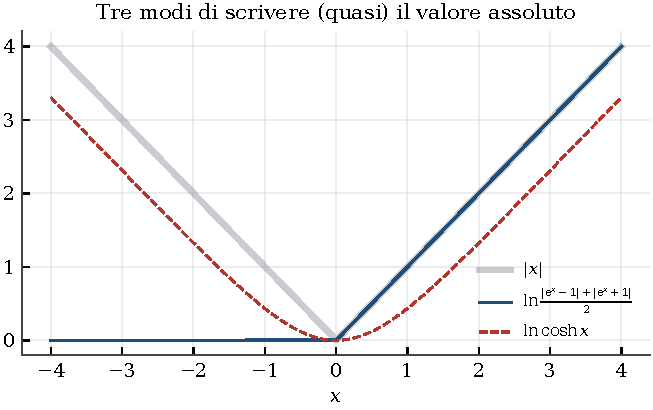
\includegraphics[width=0.86\linewidth]{../figures/mate_logcosh.pdf}
  \caption{Il meccanismo delle righe $\#77$--$\#81$: la media $\left(\left|\mathrm{e}^x-1\right|+\left|\mathrm{e}^x+1\right|\right)/2$ vale $\max\!\left(\mathrm{e}^x,1\right)$, e il suo logaritmo è $\max(x,0)$. Per confronto, $\ln\cosh x$ approssima $|x|$ ma non lo raggiunge mai.}
  \label{fig:mate_logcosh}
\end{figure}
\begin{espr}{82}{User}{}
\[
\frac{1}{2}\, \left(1 - \operatorname{sgn}\!\left(\sin\!\left(\pi\, \left(x - 1\right)\right)\right)\right)
\]
\end{espr}
Un'onda quadra costruita direttamente con la funzione segno.

\begin{espr}{83}{User}{}
\[
\frac{\ln\!\left(\frac{\left|\mathrm{e}^{\sin\!\left(\pi\, x\right)} - 1\right| + \left|\mathrm{e}^{\sin\!\left(\pi\, x\right)} + 1\right|}{2}\right)}{\sin\!\left(\pi\, x\right)}
\]
\end{espr}
Il gradino composto con il seno: onda quadra di periodo $2$.

\begin{espr}{84}{User}{}
\[
\frac{\ln\!\left(\frac{\left|\mathrm{e}^{\cos\!\left(\pi\, x\right)} - 1\right| + \left|\mathrm{e}^{\cos\!\left(\pi\, x\right)} + 1\right|}{2}\right)}{\cos\!\left(\pi\, x\right)}
\]
\end{espr}
Il gradino composto con il coseno: la stessa onda sfasata.


La chiave è l'identità $\frac{|u-1|+|u+1|}{2}=\max(|u|,1)$, vera per ogni reale $u$. Ponendo $u=\mathrm{e}^x$, che è sempre positivo, si ottiene $\max\left(\mathrm{e}^x,1\right)=\mathrm{e}^{\max(x,0)}$, e quindi
\[
  \frac{1}{x}\ln\frac{\left|\mathrm{e}^x-1\right|+\left|\mathrm{e}^x+1\right|}{2}
  =\frac{\max(x,0)}{x}
  =\begin{cases}1 & x>0\\ 0 & x<0.\end{cases}
\]
È il gradino di Heaviside, riga $\#77$. La riga $\#80$ raddoppia l'argomento e sottrae uno, ottenendo $2\max(x,0)/x-1=\mathrm{sgn}(x)$: è la funzione segno della riga $\#79$. La verifica numerica conferma entrambe esattamente. Le righe $\#83$ e $\#84$ compongono il gradino con seno e coseno e producono onde quadre.

\section{Onde triangolari e a dente di sega}

Il filone prosegue con le funzioni periodiche non sinusoidali, costruite componendo una funzione trigonometrica con l'inversa di un'altra. È il trucco che permette di ottenere spigoli da funzioni lisce.

\begin{espr}{85}{User}{}
\[
\operatorname{tri}\!\left(x\right)
\]
\end{espr}
La funzione triangolare predefinita di Derive, per confronto.

\begin{espr}{86}{User}{}
\[
\frac{1}{\pi}\, \arccos\!\left(\sin\!\left(\pi\, \left(x - \frac{1}{2}\right)\right)\right)
\]
\end{espr}
L'onda triangolare costruita con arcocoseno e seno.

\begin{espr}{87}{User}{}
\[
\left|\frac{2}{\pi}\, \arcsin\!\left(\cos\!\left(\frac{\pi\, x}{2}\right)\right)\right|
\]
\end{espr}
La stessa onda costruita con arcoseno e coseno: le due espressioni coincidono punto per punto.

\begin{espr}{88}{User}{}
\[
\left|\frac{2}{\pi}\, \arctan\!\left(\cot\!\left(\frac{\pi\, x}{2}\right)\right)\right|
\]
\end{espr}
Una terza variante con arcotangente e cotangente.

\begin{espr}{89}{User}{}
\[
\frac{4\, \arcsin^{2}\!\left(\cos\!\left(\frac{\pi\, x}{2}\right)\right)}{\pi\, \arcsin\!\left(\cos\!\left(\pi\, x\right)\right) + \frac{\pi^{2}}{2}}
\]
\end{espr}
Una combinazione quadratica delle precedenti.

\begin{espr}{90}{User}{}
\[
\operatorname{mod}\!\left(x\right)
\]
\end{espr}
La parte frazionaria secondo Derive.

\begin{espr}{91}{User}{}
\[
1 + \sum_{k=-\infty}^{+\infty} \frac{\mathrm{i}\, \mathrm{e}^{\mathrm{i}\, k\, \pi\, t}}{k\, \pi}
\]
\end{espr}
La serie di Fourier del dente di sega, in forma esponenziale bilatera.

\begin{espr}{92}{User}{}
\[
\frac{1}{\pi}\, \operatorname{arccot}\!\left(\tan\!\left(-\pi\, \left(x + \frac{1}{2}\right)\right)\right)
\]
\end{espr}
Il dente di sega costruito con arcocotangente e tangente.

\begin{espr}{93}{User}{}
\[
\frac{1}{\pi}\, \operatorname{arccot}\!\left(\tan\!\left(-\pi\, \left(x - \frac{1}{2}\right)\right)\right)
\]
\end{espr}
La stessa onda traslata di mezzo periodo.

\begin{figure}[htbp]
  \centering
  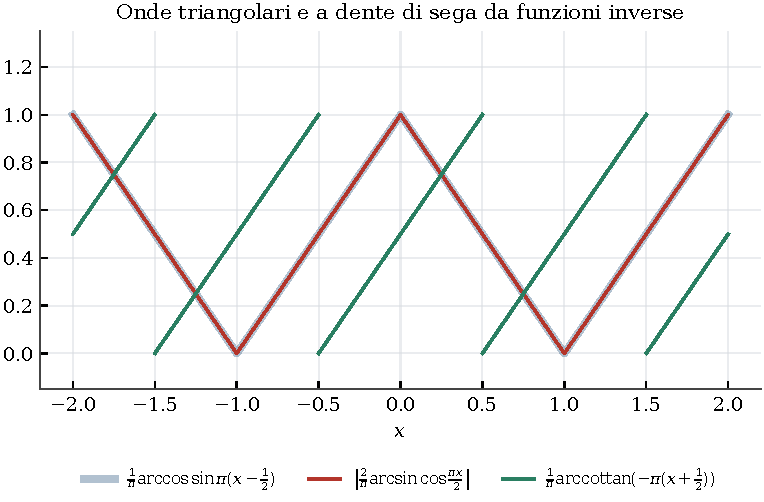
\includegraphics[width=0.86\linewidth]{../figures/mate_onde.pdf}
  \caption{Le tre costruzioni delle righe $\#86$, $\#87$ e $\#92$. Le prime due danno la stessa onda triangolare — la curva blu spessa è nascosta sotto la rossa — mentre la terza dà il dente di sega.}
  \label{fig:mate_onde}
\end{figure}
\begin{espr}{94}{User}{}
\[
-\log\!\left(\frac{1}{\pi}\, \operatorname{arccot}\!\left(\tan\!\left(\pi\, \left(x + \frac{1}{2}\right)\right)\right)\right)
\]
\end{espr}
Il logaritmo del dente di sega, cambiato di segno.

\begin{espr}{95}{User}{}
\[
-\log\!\left(\frac{1}{\pi}\, \arccos\!\left(\sin\!\left(\pi\, \left(x - \frac{1}{2}\right)\right)\right)\right)
\]
\end{espr}
L'analogo con l'onda triangolare.

\begin{espr}{96}{User}{}
\[
\arccos\!\left(\sin\!\left(-\log\!\left(\frac{1}{\pi}\, \arccos\!\left(\sin\!\left(\pi\, \left(x - \frac{1}{2}\right)\right)\right)\right)\right)\right)
\]
\end{espr}
Una composizione ulteriore.

\begin{espr}{97}{User}{}
\[
\frac{\sin\!\left(x\right)}{x}\, \left(\frac{1}{\pi}\, \operatorname{arccot}\!\left(\tan\!\left(-\pi\, \left(x + \frac{1}{2}\right)\right)\right)\right)
\]
\end{espr}
Il seno cardinale modulato dal dente di sega.

\begin{espr}{98}{User}{}
\[
\sin\!\left(\arccos\!\left(\arcsin\!\left(\cos\!\left(x + \frac{\pi}{2}\right)\right)\right)\right)
\]
\end{espr}
Una catena di funzioni inverse che si semplifica.

\begin{espr}{99}{User}{}
\[
\frac{\sin\!\left(x\right)}{x}\, \left(\frac{1}{\pi}\, \operatorname{arccot}\!\left(\tan^{2}\!\left(-\pi\, \left(x + \frac{1}{2}\right)\right)\right)\right)
\]
\end{espr}
Variante con il dente di sega al quadrato.

\begin{espr}{100}{User}{}
\[
\frac{4\, \arcsin^{2}\!\left(\cos\!\left(x\right)\right)}{\pi}\, \left(\arcsin\!\left(\cos\!\left(2\, x\right)\right) + \frac{\pi}{2}\right)
\]
\end{espr}
Una combinazione di arcoseni di coseni.

\begin{espr}{101}{User}{}
\[
\frac{2\, \arcsin\!\left(\cos^{2}\!\left(\frac{\pi\, x}{2}\right)\right)}{\arcsin\!\left(\cos\!\left(\pi\, x\right)\right) + \frac{\pi}{2}}
\]
\end{espr}
Un'altra, con argomenti dimezzati.

\begin{espr}{102}{Dif(\#94,x)}{}
\[
\frac{\mathrm{d}}{\mathrm{d}x}\!\left[-\log\!\left(\frac{1}{\pi}\, \operatorname{arccot}\!\left(\tan\!\left(\pi\, \left(x + \frac{1}{2}\right)\right)\right)\right)\right]
\]
\end{espr}
Si deriva la riga $\#94$.

\begin{espr}{103}{Simp(Dif(\#94,x))}{}
\[
\frac{1}{1 - \operatorname{mod}\!\left(x\right)}
\]
\end{espr}
Il risultato è $1/(1-\{x\})$: una funzione con asintoto verticale a ogni intero.


Le prime due costruzioni, $\#86$ e $\#87$, danno la stessa onda triangolare di periodo $2$ che vale $1$ sugli interi pari e $0$ su quelli dispari: si verifica punto per punto che coincidono. La riga $\#92$ dà invece il dente di sega, cioè la parte frazionaria, e la riga $\#90$ nomina la funzione che Derive usa allo stesso scopo.

La riga $\#91$ è la serie di Fourier del dente di sega, scritta in forma esponenziale complessa bilatera. Le righe $\#102$ e $\#103$ chiudono il filone in modo elegante: derivando il logaritmo del dente di sega si ottiene $1/(1-\{x\})$, dove $\{x\}$ è la parte frazionaria — una funzione che ha un asintoto verticale a ogni intero.

\section{Il dente di sega passa per il piano complesso}

Sette righe che rifanno la stessa costruzione con le funzioni iperboliche inverse, cioè spostandola sull'asse immaginario, e ne separano parte reale e parte immaginaria.

\begin{espr}{104}{User}{\verificata}
\begin{align*}
& \frac{2}{\pi}\, \operatorname{arcoth}\!\left(\tan\!\left(-\pi\, \left(x + \frac{1}{2}\right)\right)\right) \\
=\;& \frac{-2\, \mathrm{i}\, \operatorname{arccot}\!\left(-\mathrm{i}\, \cot\!\left(\pi\, x\right)\right)}{\pi}
\end{align*}
\end{espr}
La versione iperbolica del dente di sega, e la sua riscrittura come arcocotangente di argomento immaginario.

\begin{espr}{105}{User}{}
\[
\operatorname{Re}\!\left(\frac{-2\, \mathrm{i}\, \operatorname{arccot}\!\left(-\mathrm{i}\, \cot\!\left(\pi\, x\right)\right)}{\pi}\right)
\]
\end{espr}
Se ne chiede la parte reale.

\begin{espr}{106}{User}{\verificata}
\begin{align*}
& -\frac{\ln\!\left(\frac{1 - 2\, \sin\!\left(\pi\, x\right)\, \cos\!\left(\pi\, x\right)}{2\, \sin\!\left(\pi\, x\right)\, \cos\!\left(\pi\, x\right) + 1}\right)}{2\, \pi} \\
=\;& -\frac{\ln\!\left(\frac{1 - \sin\!\left(2\, \pi\, x\right)}{1 + \sin\!\left(2\, \pi\, x\right)}\right)}{2\, \pi}
\end{align*}
\end{espr}
Che vale un logaritmo di un rapporto in $\sin2\pi x$: due scritture equivalenti dello stesso risultato.

\begin{espr}{107}{User}{}
\[
-\operatorname{Im}\!\left(\frac{-2\, \mathrm{i}\, \operatorname{arccot}\!\left(-\mathrm{i}\, \cot\!\left(\pi\, x\right)\right)}{\pi}\right)
\]
\end{espr}
Se ne chiede la parte immaginaria, cambiata di segno.

\begin{espr}{108}{User}{}
\begin{align*}
& -\frac{\operatorname{sgn}\!\left(\sin\!\left(\pi\, x\right)\, \left(\cos\!\left(\pi\, x\right) + \sin\!\left(\pi\, x\right)\right)\right)}{2} - \frac{\operatorname{sgn}\!\left(\sin\!\left(\pi\, x\right)\, \left(\cos\!\left(\pi\, x\right) - \sin\!\left(\pi\, x\right)\right)\right)}{2} \\
&\qquad + 1
\end{align*}
\end{espr}
Che è una combinazione di funzioni segno: una scala a gradini.

\begin{espr}{109}{User}{\verificata}
\begin{align*}
& \frac{+\sin\!\left(\pi\, x\right)\, \left(\sin\!\left(\pi\, x\right) + \cos\!\left(\pi\, x\right)\right)}{2} + \frac{\sin\!\left(\pi\, x\right)\, \left(\sin\!\left(\pi\, x\right) - \cos\!\left(\pi\, x\right)\right)}{2} \\
&\qquad - \frac{1}{2} \\
=\;& \sin^{2}\!\left(\pi\, x\right) - \frac{1}{2}
\end{align*}
\end{espr}
Verifica algebrica intermedia.

\begin{espr}{110}{User}{\verificata}
\begin{align*}
& +\sin\!\left(\pi\, x\right)\, \left(\sin\!\left(\pi\, x\right) + \cos\!\left(\pi\, x\right)\right) + \sin\!\left(\pi\, x\right)\, \left(\sin\!\left(\pi\, x\right) - \cos\!\left(\pi\, x\right)\right) \\
&\qquad - 1 \\
=\;& 2\, \sin^{2}\!\left(\pi\, x\right) - 1 \\
=\;& -\cos\!\left(2\, \pi\, x\right)
\end{align*}
\end{espr}
La verifica completa: i termini misti si cancellano e resta $2\sin^2(\pi x)-1=-\cos(2\pi x)$.


La parte reale, riga $\#106$, è $-\frac{1}{2\pi}\ln\frac{1-\sin2\pi x}{1+\sin2\pi x}$: una funzione periodica con singolarità logaritmiche. La parte immaginaria, riga $\#108$, è una combinazione di funzioni segno, cioè una scala. La riga $\#110$ è l'unica identità algebrica esatta del gruppo e serve da verifica: sviluppando, $2\sin^2(\pi x)-1=-\cos(2\pi x)$.

\section{Quando una funzione iperbolica è anche circolare}

Quattro domande della stessa forma: esiste un $k$, eventualmente dipendente da $x$, per cui una funzione iperbolica coincide con la corrispondente circolare di argomento riscalato?

\begin{espr}{111}{User}{}
\[
\sinh\!\left(x\right) = \sin\!\left(k\, x\right)
\]
\end{espr}
Si chiede se il seno iperbolico coincida con un seno di argomento riscalato.

\begin{espr}{112}{User}{}
\[
k = \frac{\arcsin\!\left(\frac{\mathrm{e}^{x}}{2} - \frac{\mathrm{e}^{-x}}{2}\right)}{x}
\]
\end{espr}
Il fattore di scala esiste ma dipende da $x$.

\begin{espr}{113}{User}{}
\[
\cosh\!\left(x\right) = \cos\!\left(k\, x\right)
\]
\end{espr}
Stessa domanda per il coseno.

\begin{espr}{114}{Simp(Solve(\#113,k))}{}
\begin{align*}
& k = \frac{2\, \pi}{x} + \mathrm{i}\, \left(1 - \frac{\ln\!\left(\frac{\left|\mathrm{e}^{2\, x} - 1\right|}{2} + \frac{\mathrm{e}^{2\, x}}{2} + \frac{1}{2}\right)}{x}\right) \\[3pt]
\lor\quad & k = \mathrm{i}\, \left(1 - \frac{\ln\!\left(\frac{\left|\mathrm{e}^{2\, x} - 1\right|}{2} + \frac{\mathrm{e}^{2\, x}}{2} + \frac{1}{2}\right)}{x}\right) \\[3pt]
\lor\quad & k = \mathrm{i}\, \left(\frac{\ln\!\left(\frac{\left|\mathrm{e}^{2\, x} - 1\right|}{2} + \frac{\mathrm{e}^{2\, x}}{2} + \frac{1}{2}\right)}{x} - 1\right)
\end{align*}
\end{espr}
Le soluzioni sono immaginarie: $\cosh x\geq1$ e nessun coseno di argomento reale può eguagliarlo se non in $x=0$.

\begin{espr}{115}{User}{}
\[
\tanh\!\left(x\right) = \tan\!\left(k\, x\right)
\]
\end{espr}
Per la tangente.

\begin{espr}{116}{Simp(Solve(\#115,k))}{}
\begin{align*}
& k = \frac{\arctan\!\left(\frac{\mathrm{e}^{2\, x} - 1}{\mathrm{e}^{2\, x} + 1}\right)}{x} - \frac{\pi}{x} \\[3pt]
\lor\quad & k = \frac{\arctan\!\left(\frac{\mathrm{e}^{2\, x} - 1}{\mathrm{e}^{2\, x} + 1}\right)}{x} + \frac{\pi}{x} \\[3pt]
\lor\quad & k = \frac{\arctan\!\left(\frac{\mathrm{e}^{2\, x} - 1}{\mathrm{e}^{2\, x} + 1}\right)}{x}
\end{align*}
\end{espr}
Tre rami che differiscono per multipli di $\pi/x$: la tangente è periodica.

\begin{espr}{117}{User}{}
\[
\frac{\arctan\!\left(\frac{\mathrm{e}^{2\, x} - 1}{\mathrm{e}^{2\, x} + 1}\right)}{x}
\]
\end{espr}
Il ramo principale isolato.

\begin{espr}{118}{User}{}
\[
\operatorname{arcsinh}\!\left(x\right) = \arcsin\!\left(k\, x\right)
\]
\end{espr}
Per il seno iperbolico inverso.

\begin{espr}{119}{Simp(Solve(\#118,k))}{}
\begin{align*}
& k \\
=\;& \begin{cases} \frac{\sin\!\left(\ln\!\left(\sqrt{x^{2} + 1} + x\right)\right)}{x} & \text{se } -\frac{\pi}{2} < \ln\!\left(\sqrt{x^{2} + 1} + x\right) < \frac{\pi}{2} \end{cases}
\end{align*}
\end{espr}
Il caso più pulito: $k=\sin\!\left(\operatorname{arcsinh}x\right)/x$, con la condizione che tiene l'argomento nel dominio dell'arcoseno.

\begin{espr}{120}{User}{}
\[
\frac{\sin\!\left(\ln\!\left(\sqrt{x^{2} + 1} + x\right)\right)}{x}
\]
\end{espr}
Il fattore isolato.

\begin{espr}{121}{User}{}
\[
\operatorname{artanh}\!\left(x\right) = \arctan\!\left(k\, x\right)
\]
\end{espr}
Per la tangente iperbolica inversa.

\begin{espr}{122}{Simp(Solve(\#121,k))}{}
\begin{align*}
& k \\
=\;& \begin{cases} -\frac{\tan\!\left(\mathrm{i}\, \arctan\!\left(\mathrm{i}\, x\right)\right)}{x} & \text{se } -2\, \pi < \ln\!\left(\frac{\left(x - 1\right)^{2}}{\left(x + 1\right)^{2}}\right) < 2\, \pi \end{cases}
\end{align*}
\end{espr}
La soluzione, con la stessa struttura.

\begin{espr}{123}{User}{}
\[
\ln\!\left(\frac{\left(x - 1\right)^{2}}{\left(x + 1\right)^{2}}\right)
\]
\end{espr}
L'argomento del logaritmo che vi compare.


Le risposte sono tutte della forma $k=k(x)$, cioè il fattore di scala esiste ma non è costante. Il caso più pulito è $\#118$: da $\operatorname{arcsinh}x=\arcsin(kx)$ segue $kx=\sin\!\left(\operatorname{arcsinh}x\right)$ e quindi, essendo $\operatorname{arcsinh}x=\ln\!\left(x+\sqrt{x^2+1}\right)$, si ha $k=\sin\!\left(\ln\!\left(x+\sqrt{x^2+1}\right)\right)/x$: esattamente la risposta $\#119$, con la condizione che garantisce di restare nel dominio dell'arcoseno. Il caso $\#113$ mostra invece che per il coseno il fattore è necessariamente immaginario: $\cosh x\geq1$ e $\cos$ non può superare $1$ con argomento reale.

La risposta sistematica a queste domande è la funzione gudermanniana $\operatorname{gd}x=2\arctan\left(\tanh\tfrac x2\right)$, che lega funzioni circolari e iperboliche senza passare per i numeri complessi: $\tan(\operatorname{gd}x)=\sinh x$, $\sin(\operatorname{gd}x)=\tanh x$, $\cos(\operatorname{gd}x)=1/\cosh x$. Per esempio la soluzione principale della riga $\#116$, $kx=\arctan(\tanh x)$, vale $\tfrac12\operatorname{gd}(2x)$.

\section{Arcoseno e arcocoseno di argomento complesso}

Le ultime dieci righe tornano al piano complesso con due identità di conversione e alcune espressioni miste che il quaderno lascia aperte.

\begin{espr}{124}{User}{}
\[
\arcsin\!\left(z\right) + \mathrm{i}\, \arccos\!\left(z\right) = x + \mathrm{i}\, y
\]
\end{espr}
Si pone una combinazione di arcoseno e arcocoseno uguale a un numero complesso generico.

\begin{espr}{125}{User}{}
\[
z + \sin\!\left(\mathrm{i}\, \arccos\!\left(z\right)\right) = \sin\!\left(x + \mathrm{i}\, y\right)
\]
\end{espr}
Si applica il seno a entrambi i membri.

\begin{espr}{126}{User}{}
\[
\cos\!\left(\arcsin\!\left(z\right)\right) + \cos\!\left(\mathrm{i}\, \arccos\!\left(z\right)\right) = \cos\!\left(x + \mathrm{i}\, y\right)
\]
\end{espr}
E il coseno.

\begin{espr}{127}{User}{\verificata}
\[
\cos\!\left(\mathrm{i}\, \arccos\!\left(z\right)\right) = \cosh\!\left(-\arccos\!\left(z\right)\right)
\]
\end{espr}
La regola di conversione per il coseno di argomento immaginario.

\begin{espr}{128}{User}{\verificata}
\[
\sin\!\left(\mathrm{i}\, \arccos\!\left(z\right)\right) = \frac{1}{\mathrm{i}}\, \sinh\!\left(-\arccos\!\left(z\right)\right)
\]
\end{espr}
E per il seno, con il fattore $1/\mathrm{i}$.

\begin{espr}{129}{User}{\verificata}
\[
\sin\!\left(\mathrm{i}\, \arccos\!\left(z\right)\right) = \mathrm{i}\, \sinh\!\left(\arccos\!\left(z\right)\right)
\]
\end{espr}
La stessa riga scritta con $\mathrm{i}$ al numeratore: $1/\mathrm{i}=-\mathrm{i}$ e il segno dell'argomento si compensa.

\begin{espr}{130}{User}{}
\[
\mathrm{e}^{x} + \mathrm{i}\, \mathrm{e}^{y}
\]
\end{espr}
Un'espressione mista, punto di partenza per l'ultimo gruppo.

\begin{espr}{131}{Sub(User)}{}
\[
\pi\, \mathrm{e}^{\mathrm{i}\, \left(x + \mathrm{i}\, y\right)} + \mathrm{i}\, \mathrm{e}^{\pi\, \left(x + \mathrm{i}\, y\right)}
\]
\end{espr}
Con la sostituzione $x\to x+\mathrm{i}y$ e i due esponenziali scambiati di base.

\begin{espr}{132}{User}{\verificata}
\begin{align*}
& \pi\, \mathrm{e}^{-y + \frac{\mathrm{i}\, \left(2\, x + \pi\right)}{2}} + \pi\, \mathrm{e}^{\pi\, x}\, \left(-1\right)^{\frac{2\, y + 1}{2}} \\
=\;& -\mathrm{i}\, \left(-\pi\, \mathrm{e}^{-y + \mathrm{i}\, x} - \pi\, \mathrm{e}^{\pi\, x}\, \left(-1\right)^{y}\right)
\end{align*}
\end{espr}
L'identità che ne risulta, verificata da Derive.

\begin{espr}{133}{User}{}
\[
\frac{\ln\!\left(\frac{\left|\mathrm{e}^{x} - 1\right| + \left|\mathrm{e}^{x} + 1\right|}{2}\right)}{x}
\]
\end{espr}
L'ultima riga del quaderno ripete il gradino della riga $\#77$.


Le righe $\#127$--$\#129$ sono le regole di conversione: $\cos(\mathrm{i}w)=\cosh w$ e $\sin(\mathrm{i}w)=\mathrm{i}\sinh w$, scritte con $w=\arccos z$. L'ultima riga ripete testualmente la $\#77$: il quaderno si chiude tornando al gradino, che è forse il risultato di cui l'autore era più soddisfatto.

\section*{In sintesi}
\addcontentsline{toc}{section}{In sintesi}

Il quaderno vale soprattutto per due cose. La prima è l'identità di apertura, che è vera, elementare e ripresa una quarantina di volte: il rapporto fra differenze di quadrati di coseni e differenze di coseni duplicati è la costante $1/2$, e la versione con la triplicazione dà $1/4$; la regola $2^{1-n}$ vale solo per $n=2$ e $n=3$. La seconda è la costruzione del gradino e della funzione segno con soli logaritmi e valori assoluti, che è esatta: il gradino vale $\max(x,0)/x$, perché $\left(|\mathrm{e}^x-1|+|\mathrm{e}^x+1|\right)/2=\max(\mathrm{e}^x,1)$.

In mezzo c'è una lunga sezione dedicata a interrogare un'equazione indeterminata, con la sua risposta priva di significato inseguita per trenta espressioni. Averla conservata non toglie niente al resto: mostra come questi quaderni venissero usati davvero, cioè come strumenti per provare, non per esporre.


%% generato automaticamente da tools/build_tex.py --- non modificare
\chapter{La versione di febbraio}
\label{cap:mate-copia}
\quaderno{mate copia.dfw}{09 Feb 2010}{127}

Il nome del file dice \dfw{copia}, ma le date raccontano un'altra storia: questo quaderno è del 9 febbraio 2010, mentre \dfw{mate.dfw} è del 18 agosto successivo. Non è una copia, è lo stato precedente dello stesso lavoro — sei mesi prima, e sei espressioni più corto.

Delle 127 espressioni qui contenute, 117 compaiono identiche nel quaderno di agosto (capitolo~\ref{cap:mate}), dove sono commentate una per una. Questo capitolo le riporta comunque tutte, per completezza del recupero, ma concentra il commento sulle tre che nella versione successiva sono state tolte. Sono le più interessanti, perché una scomparsa è sempre una scelta.

\section{L'identità con due pesi}

La prima espressione che verrà eliminata è anche la più generale del quaderno, e sta subito all'inizio.

\begin{espr}{1}{User}{\verificata}
\[
\frac{\cos\!\left(x\right) - \cos\!\left(y\right)}{\cos\!\left(x\right) - \cos\!\left(y\right)} = 1
\]
\end{espr}
\begin{espr}{2}{User}{\verificata}
\begin{align*}
& \frac{\cos^{2}\!\left(x\right) - \cos^{2}\!\left(y\right)}{k\, \left(\cos^{2}\!\left(x\right) - \cos^{2}\!\left(y\right)\right) - l\, \left(\sin^{2}\!\left(x\right) - \sin^{2}\!\left(y\right)\right)} \\
=\;& \frac{1}{k + l}
\end{align*}
\end{espr}
La forma generale dell'identità, con due pesi liberi al denominatore. Da qui discendono tutti i casi particolari usati nel resto della raccolta.


La riga $\#2$ è la forma generale dell'identità che regge tutto il lavoro. Al denominatore compaiono due pesi, uno per la differenza di quadrati di coseni e uno per quella di seni, e il valore del rapporto è $1/(k+l)$. Si verifica in una riga: poiché $\cos^2x-\cos^2y$ e $\sin^2x-\sin^2y$ sono uno l'opposto dell'altro, il denominatore vale $(k+l)\left(\cos^2x-\cos^2y\right)$ e il rapporto si semplifica.

Da questa forma discendono tutti i casi particolari usati nel resto del lavoro: $k=1,\ l=1$ dà $1/2$, ed è l'identità di apertura; $k=0,\ l=-1$ dà $-1$; e così via. Nella versione di agosto questa riga non c'è più, sostituita dai casi particolari scritti uno per uno. È una scelta curiosa — il caso generale era già stato trovato e poi è stato lasciato indietro.

\section{Il corpo del quaderno}

Le espressioni che seguono corrispondono, con lo scarto di qualche numero d'ordine, a quelle del capitolo~\ref{cap:mate}: l'identità del mezzo e le sue varianti, la caccia al parametro, i due parametri, la macchina per $\pi$, il gradino costruito con logaritmi e valori assoluti, le onde triangolari e a dente di sega, il confronto fra funzioni circolari e iperboliche. Per il commento si rimanda a quel capitolo.

\begin{espr}{3}{User}{\verificata}
\[
\frac{\cos^{2}\!\left(x\right) - \cos^{2}\!\left(y\right)}{\cos\!\left(2\, x\right) - \cos\!\left(2\, y\right)} = \frac{1}{2}
\]
\end{espr}
\begin{espr}{4}{User}{\verificata}
\[
\frac{\sin^{2}\!\left(x\right) - \sin^{2}\!\left(y\right)}{\cos\!\left(2\, x\right) - \cos\!\left(2\, y\right)} = -\frac{1}{2}
\]
\end{espr}
\begin{espr}{5}{User}{\verificata}
\begin{align*}
& \frac{\cos^{3}\!\left(x\right)\, \cos\!\left(y\right) - \cos^{3}\!\left(y\right)\, \cos\!\left(x\right)}{\cos\!\left(3\, x\right)\, \cos\!\left(y\right) - \cos\!\left(3\, y\right)\, \cos\!\left(x\right)} \\
=\;& \frac{\cos\!\left(x\right)\, \cos\!\left(y\right)\, \left(\cos^{2}\!\left(x\right) - \cos^{2}\!\left(y\right)\right)}{\cos\!\left(y\right)\, \cos\!\left(3\, x\right) - \cos\!\left(x\right)\, \cos\!\left(3\, y\right)} \\
=\;& \frac{1}{4}
\end{align*}
\end{espr}
\begin{espr}{6}{User}{\verificata}
\begin{align*}
& \frac{\mathrm{e}^{2\, \mathrm{i}\, x} - \mathrm{e}^{2\, \mathrm{i}\, y} + \sin^{2}\!\left(y\right) - \sin^{2}\!\left(x\right) + 2\, \mathrm{i}\, \left(\mathrm{e}^{\mathrm{i}\, y}\, \sin\!\left(y\right) - \mathrm{e}^{\mathrm{i}\, x}\, \sin\!\left(x\right)\right)}{\mathrm{e}^{2\, \mathrm{i}\, x} - \mathrm{e}^{2\, \mathrm{i}\, y} + \mathrm{i}\, \left(\sin\!\left(2\, y\right) - \sin\!\left(2\, x\right)\right)} \\
=\;& \frac{1}{2}
\end{align*}
\end{espr}
\begin{espr}{7}{User}{}
\begin{align*}
& \operatorname{Re}\!\left(\mathrm{e}^{2\, \mathrm{i}\, x} - \mathrm{e}^{2\, \mathrm{i}\, y} + \mathrm{i}\, \left(\sin\!\left(2\, y\right) - \sin\!\left(2\, x\right)\right)\right) \\
=\;& \cos\!\left(2\, x\right) - \cos\!\left(2\, y\right)
\end{align*}
\end{espr}
\begin{espr}{8}{User}{}
\begin{align*}
& \operatorname{Im}\!\left(\mathrm{e}^{2\, \mathrm{i}\, x} - \mathrm{e}^{2\, \mathrm{i}\, y} + \mathrm{i}\, \left(\sin\!\left(2\, y\right) - \sin\!\left(2\, x\right)\right)\right) \\
=\;& 0
\end{align*}
\end{espr}
\begin{espr}{9}{User}{}
\begin{align*}
& \operatorname{Re}\!\left(\mathrm{e}^{2\, \mathrm{i}\, x} - \mathrm{e}^{2\, \mathrm{i}\, y} + \sin^{2}\!\left(y\right) - \sin^{2}\!\left(x\right) + 2\, \mathrm{i}\, \left(\mathrm{e}^{\mathrm{i}\, y}\, \sin\!\left(y\right) - \mathrm{e}^{\mathrm{i}\, x}\, \sin\!\left(x\right)\right)\right) \\
=\;& \frac{\cos\!\left(2\, x\right)}{2} - \frac{\cos\!\left(2\, y\right)}{2}
\end{align*}
\end{espr}
\begin{espr}{10}{User}{}
\begin{align*}
& \operatorname{Im}\!\left(\mathrm{e}^{2\, \mathrm{i}\, x} - \mathrm{e}^{2\, \mathrm{i}\, y} + \sin^{2}\!\left(y\right) - \sin^{2}\!\left(x\right) + 2\, \mathrm{i}\, \left(\mathrm{e}^{\mathrm{i}\, y}\, \sin\!\left(y\right) - \mathrm{e}^{\mathrm{i}\, x}\, \sin\!\left(x\right)\right)\right) \\
=\;& 0
\end{align*}
\end{espr}
\begin{espr}{11}{User}{\verificata}
\begin{align*}
& \cos\!\left(5\, x\right) \\
=\;& \left(\cos\!\left(x\right)\, \cos\!\left(2\, x\right) - \sin\!\left(x\right)\, \sin\!\left(2\, x\right)\right)\, \cos\!\left(2\, x\right) - \sin\!\left(2\, x\right)\, \left(\sin\!\left(x\right)\, \cos\!\left(2\, x\right) + \sin\!\left(2\, x\right)\, \cos\!\left(x\right)\right)
\end{align*}
\end{espr}
\begin{espr}{12}{User}{\verificata}
\[
\cos\!\left(5\, x\right) = \cos\!\left(x\right)\, \cos\!\left(4\, x\right) - \sin\!\left(x\right)\, \sin\!\left(4\, x\right)
\]
\end{espr}
\begin{espr}{13}{Solve(User,[f,m,s])}{}
\[
\operatorname{Solve}\!\left(\left[\, f^{2} + m^{2} = 0,\; f\, m = 1,\; s = \frac{1}{2}\, \left(f + m\right) \,\right],\; \left[\, f,\; m,\; s \,\right]\right)
\]
\end{espr}
\begin{espr}{14}{Simp(Solve(User,[f,m,s]))}{}
\[
\left[\, f = \frac{\sqrt{2}}{2} + \frac{\sqrt{2}\, \mathrm{i}}{2} \;\land\; m = \frac{\sqrt{2}}{2} - \frac{\sqrt{2}\, \mathrm{i}}{2} \;\land\; s = \frac{\sqrt{2}}{2},\; f = \frac{\sqrt{2}}{2} - \frac{\sqrt{2}\, \mathrm{i}}{2} \;\land\; m = \frac{\sqrt{2}}{2} + \frac{\sqrt{2}\, \mathrm{i}}{2} \;\land\; s = \frac{\sqrt{2}}{2},\; f = -\frac{\sqrt{2}}{2} + \frac{\sqrt{2}\, \mathrm{i}}{2} \;\land\; m = -\frac{\sqrt{2}}{2} - \frac{\sqrt{2}\, \mathrm{i}}{2} \;\land\; s = -\frac{\sqrt{2}}{2},\; f = -\frac{\sqrt{2}}{2} - \frac{\sqrt{2}\, \mathrm{i}}{2} \;\land\; m = -\frac{\sqrt{2}}{2} + \frac{\sqrt{2}\, \mathrm{i}}{2} \;\land\; s = -\frac{\sqrt{2}}{2} \,\right]
\]
\end{espr}
\begin{espr}{15}{User}{}
\[
\frac{n\, \sin^{x}\!\left(\pi\, x\right)}{\pi\, x}
\]
\end{espr}
\begin{espr}{16}{User}{}
\[
\frac{\sin\!\left(\mathrm{e}\, x\right)}{\mathrm{e}\, x}
\]
\end{espr}
\begin{espr}{17}{User}{}
\[
\frac{n\, \sin\!\left(\mathrm{e}\, x\right)}{\mathrm{e}\, x}
\]
\end{espr}
\begin{espr}{18}{User}{}
\[
\lim_{n \to \infty} \frac{n\, \sin\!\left(\mathrm{e}\, x\right)}{\mathrm{e}\, x}
\]
\end{espr}
\begin{espr}{19}{User}{}
\[
\frac{\cos^{2}\!\left(x + \mathrm{i}\, y\right) - \cos^{2}\!\left(x - \mathrm{i}\, y\right)}{\cos\!\left(2\, x + 2\, \mathrm{i}\, y\right) - \cos\!\left(2\, x - 2\, \mathrm{i}\, y\right)}
\]
\end{espr}
\begin{espr}{20}{Simp(\#19)}{}
\[
\frac{1}{2}
\]
\end{espr}
\begin{espr}{21}{User}{\verificata}
\begin{align*}
& \frac{\cos^{2}\!\left(x + k\, y\right) - \cos^{2}\!\left(x - k\, y\right)}{\cos\!\left(2\, x + 2\, k\, y\right) - \cos\!\left(2\, x - 2\, k\, y\right)} \\
=\;& \frac{1}{2}
\end{align*}
\end{espr}
\begin{espr}{22}{Solve(\#21,k)}{}
\[
\operatorname{Approx}\!\left(\operatorname{Solve}\!\left(\frac{\cos^{2}\!\left(x + k\, y\right) - \cos^{2}\!\left(x - k\, y\right)}{\cos\!\left(2\, x + 2\, k\, y\right) - \cos\!\left(2\, x - 2\, k\, y\right)} = \frac{1}{2},\; k\right)\right)
\]
\end{espr}
\begin{espr}{23}{Simp(Solve(\#21,k))}{}
\[
k = -4.999999701
\]
\end{espr}
\begin{espr}{24}{User}{\verificata}
\begin{align*}
& \frac{\cos^{2}\!\left(x + \mathrm{i}\, y\right) - \cos^{2}\!\left(x - \mathrm{i}\, y\right)}{\cos\!\left(2\, x + 2\, \mathrm{i}\, y\right) - \cos\!\left(2\, x - 2\, \mathrm{i}\, y\right)} \\
=\;& \frac{1}{2}
\end{align*}
\end{espr}
\begin{espr}{25}{User}{\verificata}
\begin{align*}
& \frac{\cos^{2}\!\left(x + k\, y\right) - \cos^{2}\!\left(k\, y\right)}{\cos\!\left(2\, x + 2\, k\, y\right) - \cos\!\left(2\, k\, y\right)} \\
=\;& \frac{1}{2}
\end{align*}
\end{espr}
\begin{espr}{26}{Solve(\#25,k)}{}
\[
\operatorname{Approx}\!\left(\operatorname{Solve}\!\left(\frac{\cos^{2}\!\left(x + k\, y\right) - \cos^{2}\!\left(k\, y\right)}{\cos\!\left(2\, x + 2\, k\, y\right) - \cos\!\left(2\, k\, y\right)} = \frac{1}{2},\; k\right)\right)
\]
\end{espr}
\begin{espr}{27}{Simp(Solve(\#25,k))}{}
\[
k = -4.999999701
\]
\end{espr}
\begin{espr}{28}{User}{\verificata}
\[
\frac{\cos^{2}\!\left(3\, x + k\, y\right) - \cos^{2}\!\left(x\right)}{\cos\!\left(6\, x + 2\, k\, y\right) - \cos\!\left(2\, x\right)} = \frac{1}{2}
\]
\end{espr}
\begin{espr}{29}{Solve(\#28,k)}{}
\[
\operatorname{Approx}\!\left(\operatorname{Solve}\!\left(\frac{\cos^{2}\!\left(3\, x + k\, y\right) - \cos^{2}\!\left(x\right)}{\cos\!\left(6\, x + 2\, k\, y\right) - \cos\!\left(2\, x\right)} = \frac{1}{2},\; k\right)\right)
\]
\end{espr}
\begin{espr}{30}{Simp(\#29)}{}
\[
k = -4.999999701
\]
\end{espr}
\begin{espr}{31}{User}{\verificata}
\[
\frac{\cos^{2}\!\left(x + k\right) - \cos^{2}\!\left(x - k\right)}{\cos\!\left(2\, x + 2\, k\right) - \cos\!\left(2\, x - 2\, k\right)} = \frac{1}{2}
\]
\end{espr}
\begin{espr}{32}{Solve(\#31,k)}{}
\[
\operatorname{Approx}\!\left(\operatorname{Solve}\!\left(\frac{\cos^{2}\!\left(x + k\right) - \cos^{2}\!\left(x - k\right)}{\cos\!\left(2\, x + 2\, k\right) - \cos\!\left(2\, x - 2\, k\right)} = \frac{1}{2},\; k,\; \mathrm{Real}\right)\right)
\]
\end{espr}
\begin{espr}{33}{Simp(Solve(\#31,k))}{}
\[
k = -4.999999701
\]
\end{espr}
\begin{espr}{34}{User}{\verificata}
\begin{align*}
& \frac{\cos^{3}\!\left(x\right)\, \cos\!\left(y\right) - \cos^{3}\!\left(y\right)\, \cos\!\left(x\right)}{\cos\!\left(3\, x\right)\, \cos\!\left(y\right) - \cos\!\left(3\, y\right)\, \cos\!\left(x\right)} \\
=\;& \frac{\cos\!\left(x\right)\, \cos\!\left(y\right)\, \left(\cos^{2}\!\left(x\right) - \cos^{2}\!\left(y\right)\right)}{\cos\!\left(y\right)\, \cos\!\left(3\, x\right) - \cos\!\left(x\right)\, \cos\!\left(3\, y\right)} \\
=\;& \frac{1}{4}
\end{align*}
\end{espr}
\begin{espr}{35}{User}{\verificata}
\begin{align*}
& \frac{\cos\!\left(x + k\, y\right)\, \cos\!\left(x - k\, y\right)\, \left(\cos^{2}\!\left(x + k\, y\right) - \cos^{2}\!\left(x - k\, y\right)\right)}{\cos\!\left(x - k\, y\right)\, \cos\!\left(3\, x + 3\, k\, y\right) - \cos\!\left(x + k\, y\right)\, \cos\!\left(3\, x - 3\, k\, y\right)} \\
=\;& \frac{1}{4}
\end{align*}
\end{espr}
\begin{espr}{36}{Solve(\#35,k)}{}
\[
\operatorname{Approx}\!\left(\operatorname{Solve}\!\left(\frac{\cos\!\left(x + k\, y\right)\, \cos\!\left(x - k\, y\right)\, \left(\cos^{2}\!\left(x + k\, y\right) - \cos^{2}\!\left(x - k\, y\right)\right)}{\cos\!\left(x - k\, y\right)\, \cos\!\left(3\, x + 3\, k\, y\right) - \cos\!\left(x + k\, y\right)\, \cos\!\left(3\, x - 3\, k\, y\right)} = \frac{1}{4},\; k\right)\right)
\]
\end{espr}
\begin{espr}{37}{Simp(Solve(\#35,k))}{}
\[
k = 0
\]
\end{espr}
\begin{espr}{38}{User}{}
\[
\frac{\cos\!\left(x\right)\, \cos\!\left(y\right)\, \left(\cos^{2}\!\left(x\right) - \cos^{2}\!\left(y\right)\right)}{\cos\!\left(y\right)\, \cos\!\left(3\, x\right) - \cos\!\left(x\right)\, \cos\!\left(3\, y\right)}
\]
\end{espr}
\begin{espr}{39}{User}{\verificata}
\begin{align*}
& \frac{\cos^{2}\!\left(x + k\, y\right) - \cos^{2}\!\left(x - k\, y\right)}{\cos\!\left(2\, x + 2\, k\, y\right) - \cos\!\left(2\, x - 2\, k\, y\right)} \\
=\;& \frac{1}{2}
\end{align*}
\end{espr}
\begin{espr}{40}{User}{\verificata}
\begin{align*}
& \frac{\cos^{2}\!\left(x - 4.999999701\, y\right) - \cos^{2}\!\left(x + 4.999999701\, y\right)}{\cos\!\left(2\, x - 2 \cdot 4.999999701\, y\right) - \cos\!\left(2\, x + 2 \cdot 4.999999701\, y\right)} \\
=\;& \frac{1}{2}
\end{align*}
\end{espr}
\begin{espr}{41}{User}{\verificata}
\[
\frac{\cos^{2}\!\left(x\right) - \cos^{2}\!\left(y\right)}{\cos\!\left(2\, x\right) - \cos\!\left(2\, y\right)} = \frac{1}{2}
\]
\end{espr}
\begin{espr}{42}{User}{\verificata}
\[
\frac{\cos^{2}\!\left(x + y\right) - \cos^{2}\!\left(x - y\right)}{\cos\!\left(2\, x + 2\, y\right) - \cos\!\left(2\, x - 2\, y\right)} = \frac{1}{2}
\]
\end{espr}
\begin{espr}{43}{Simp(Solve(User,y))}{}
\[
y = -4.999999701
\]
\end{espr}
\begin{espr}{44}{User}{\verificata}
\begin{align*}
& \frac{\cos\!\left(x + y\right)\, \cos\!\left(x - y\right)\, \left(\cos^{2}\!\left(x + y\right) - \cos^{2}\!\left(x - y\right)\right)}{\cos\!\left(x - y\right)\, \cos\!\left(3\, x + 3\, y\right) - \cos\!\left(x + y\right)\, \cos\!\left(3\, x - 3\, y\right)} \\
=\;& \frac{1}{4}
\end{align*}
\end{espr}
\begin{espr}{45}{User}{}
\[
y = -2.499998615
\]
\end{espr}
\begin{espr}{46}{User}{}
\[
k\, 3.141592654 = -4.999999701
\]
\end{espr}
\begin{espr}{47}{Solve(\#46,k)}{}
\[
\operatorname{Approx}\!\left(\operatorname{Solve}\!\left(k\, 3.141592654 = -4.999999701,\; k,\; \mathrm{Real}\right)\right)
\]
\end{espr}
\begin{espr}{48}{Simp(Solve(\#46,k))}{}
\[
k = -1.591549335
\]
\end{espr}
\begin{espr}{49}{User}{\verificata}
\[
\frac{\cos^{2}\!\left(x\right) - \cos^{2}\!\left(y\right)}{\cos\!\left(2\, x\right) - \cos\!\left(2\, y\right)} = \frac{1}{2}
\]
\end{espr}
\begin{espr}{50}{User}{}
\[
\cos^{2}\!\left(x\right) - \cos^{2}\!\left(y\right) = 1
\]
\end{espr}
\begin{espr}{51}{User}{}
\[
\cos\!\left(2\, x\right) - \cos\!\left(2\, y\right) = 2
\]
\end{espr}
\begin{espr}{52}{Solve(User,[j,k])}{}
\[
\operatorname{Solve}\!\left(\left[\, \cos^{2}\!\left(k\right) - \cos^{2}\!\left(j\right) = 1,\; \cos\!\left(2\, k\right) - \cos\!\left(2\, j\right) = 2 \,\right],\; \left[\, j,\; k \,\right]\right)
\]
\end{espr}
\begin{espr}{53}{User}{}
\[
\frac{\cos^{2}\!\left(x\right) - k\, \cos^{2}\!\left(y\right)}{\cos\!\left(2\, x\right) - l\, \cos\!\left(2\, y\right)} = \frac{1}{2}
\]
\end{espr}
\begin{espr}{54}{Simp(Solve(\#53,k))}{}
\[
k = \frac{l\, \cos\!\left(2\, y\right) + 1}{2\, \cos^{2}\!\left(y\right)}
\]
\end{espr}
\begin{espr}{55}{Simp(Solve(\#53,l))}{}
\[
l = \frac{2\, k\, \cos^{2}\!\left(y\right) - 1}{\cos\!\left(2\, y\right)}
\]
\end{espr}
\begin{espr}{56}{User}{}
\[
\operatorname{Solve}\!\left(\left[\, k = \frac{l\, \cos\!\left(2\, y\right) + 1}{2\, \cos^{2}\!\left(y\right)},\; l = \frac{2\, k\, \cos^{2}\!\left(y\right) - 1}{\cos\!\left(2\, y\right)} \,\right],\; \left[\, k,\; l \,\right]\right)
\]
\end{espr}
\begin{espr}{57}{Simp(Solve(User,[k,l]))}{}
\[
\left[\, \frac{\left(k - l\right)\, \cos\!\left(2\, y\right) + k}{\cos\!\left(2\, y\right) + 1} = \frac{1}{\cos\!\left(2\, y\right) + 1} \,\right]
\]
\end{espr}
\begin{espr}{58}{Solve(\#57,k)}{}
\[
\operatorname{Solve}\!\left(\left[\, \frac{\left(k - l\right)\, \cos\!\left(2\, y\right) + k}{\cos\!\left(2\, y\right) + 1} = \frac{1}{\cos\!\left(2\, y\right) + 1} \,\right],\; k\right)
\]
\end{espr}
\begin{espr}{59}{Simp(Solve(\#57,k))}{}
\[
\left[\, k = \frac{l\, \cos\!\left(2\, y\right) + 1}{\cos\!\left(2\, y\right) + 1} \,\right]
\]
\end{espr}
\begin{espr}{60}{User}{}
\[
\cos\!\left(2\, y\right) = \frac{1 - k}{k - l}
\]
\end{espr}
\begin{espr}{61}{User}{}
\begin{align*}
& \frac{\cos^{2}\!\left(x\right) - x\, \left(1 + k\right)\, \cos^{2}\!\left(y\right)}{\cos\!\left(2\, x\right) - y\, \left(1 + k\right)\, \cos\!\left(2\, y\right)} \\
=\;& \frac{1}{2}
\end{align*}
\end{espr}
\begin{espr}{62}{Simp(Solve(\#61,k))}{}
\[
k = -\frac{\left(x - y\right)\, \cos\!\left(2\, y\right) + x - 1}{\left(x - y\right)\, \cos\!\left(2\, y\right) + x}
\]
\end{espr}
\begin{espr}{63}{User}{}
\begin{align*}
& \frac{\cos^{2}\!\left(x\right) - \left(1 + k\right)\, \cos^{2}\!\left(y\right)}{\cos\!\left(2\, x\right) - \left(1 + k\right)\, \cos\!\left(2\, y\right)} \\
=\;& \frac{k}{2}
\end{align*}
\end{espr}
\begin{espr}{64}{Solve(\#63,k)}{}
\[
\operatorname{Solve}\!\left(\frac{\cos^{2}\!\left(x\right) - \left(1 + k\right)\, \cos^{2}\!\left(y\right)}{\cos\!\left(2\, x\right) - \left(1 + k\right)\, \cos\!\left(2\, y\right)} = \frac{k}{2},\; k\right)
\]
\end{espr}
\begin{espr}{65}{Simp(Solve(\#63,k))}{}
\begin{align*}
& k = -\frac{\sqrt{\cos^{2}\!\left(2\, x\right) + 2\, \cos\!\left(2\, x\right)\, \left(1 - 2\, \cos\!\left(2\, y\right)\right) + 4\, \cos^{2}\!\left(2\, y\right) + 1}}{2\, \cos\!\left(2\, y\right)} + \frac{\cos\!\left(2\, x\right)}{2\, \cos\!\left(2\, y\right)} + \frac{1}{2\, \cos\!\left(2\, y\right)} \\[3pt]
\lor\quad & k = \frac{\sqrt{\cos^{2}\!\left(2\, x\right) + 2\, \cos\!\left(2\, x\right)\, \left(1 - 2\, \cos\!\left(2\, y\right)\right) + 4\, \cos^{2}\!\left(2\, y\right) + 1}}{2\, \cos\!\left(2\, y\right)} + \frac{\cos\!\left(2\, x\right)}{2\, \cos\!\left(2\, y\right)} + \frac{1}{2\, \cos\!\left(2\, y\right)}
\end{align*}
\end{espr}
\begin{espr}{66}{User}{}
\[
\frac{1}{\pi}\, \left(y - x\right)\, \left(x + \frac{1}{y}\right)
\]
\end{espr}
\begin{espr}{67}{User}{\verificata}
\[
\left(\frac{1}{2}\right)! = \frac{\sqrt{\pi}}{2}
\]
\end{espr}
\begin{espr}{68}{User}{\verificata}
\[
4\, \left(\frac{1}{2}\right)!^{2} = \pi
\]
\end{espr}
\begin{espr}{69}{User}{}
\[
\cos\!\left(x\right)!
\]
\end{espr}
\begin{espr}{70}{User}{\verificata}
\[
\left(\frac{\cos^{2}\!\left(x\right) - \cos^{2}\!\left(y\right)}{\cos\!\left(2\, x\right) - \cos\!\left(2\, y\right)}\right)! = \frac{\sqrt{\pi}}{2}
\]
\end{espr}
\begin{espr}{71}{User}{\verificata}
\[
4\, \left(\frac{\cos^{2}\!\left(x\right) - \cos^{2}\!\left(y\right)}{\cos\!\left(2\, x\right) - \cos\!\left(2\, y\right)}\right)!^{2} = \pi
\]
\end{espr}
\begin{espr}{72}{User}{\verificata}
\[
\arccos\!\left(\frac{x}{\pi}\right) + \arcsin\!\left(\frac{x}{\pi}\right) = \frac{\pi}{2}
\]
\end{espr}
\begin{espr}{73}{User}{\verificata}
\[
\sin\!\left(\arccos\!\left(x\right)\right) = \cos\!\left(\arcsin\!\left(x\right)\right)
\]
\end{espr}
\begin{espr}{74}{User}{}
\[
\arccos\!\left(\sin\!\left(x\right)\right)
\]
\end{espr}
\begin{espr}{75}{User}{}
\[
\arcsin\!\left(\cos\!\left(x\right)\right)
\]
\end{espr}
\begin{espr}{76}{User}{}
\[
\operatorname{sgn}\!\left(x\right)
\]
\end{espr}
\begin{espr}{77}{User}{}
\[
\frac{\ln\!\left(\frac{\left|\mathrm{e}^{2\, x} - 1\right| + \left|\mathrm{e}^{2\, x} + 1\right|}{2}\right)}{x} - 1
\]
\end{espr}
\begin{espr}{78}{User}{}
\[
\frac{2\, \ln\!\left(\frac{\left|\mathrm{e}^{x} - 1\right| + \left|\mathrm{e}^{x} + 1\right|}{2}\right)}{x} - 1
\]
\end{espr}
\begin{espr}{79}{User}{}
\[
\operatorname{tri}\!\left(x\right)
\]
\end{espr}
\begin{espr}{80}{User}{}
\[
\frac{1}{\pi}\, \arccos\!\left(\sin\!\left(\pi\, \left(x - \frac{1}{2}\right)\right)\right)
\]
\end{espr}
\begin{espr}{81}{User}{}
\[
\left|\frac{2}{\pi}\, \arcsin\!\left(\cos\!\left(\frac{\pi\, x}{2}\right)\right)\right|
\]
\end{espr}
\begin{espr}{82}{User}{}
\[
\left|\frac{2}{\pi}\, \arctan\!\left(\cot\!\left(\frac{\pi\, x}{2}\right)\right)\right|
\]
\end{espr}
\begin{espr}{83}{User}{}
\[
\frac{4\, \arcsin^{2}\!\left(\cos\!\left(\frac{\pi\, x}{2}\right)\right)}{\pi\, \arcsin\!\left(\cos\!\left(\pi\, x\right)\right) + \frac{\pi^{2}}{2}}
\]
\end{espr}
\begin{espr}{84}{User}{}
\[
\operatorname{mod}\!\left(x\right)
\]
\end{espr}
\begin{espr}{85}{User}{}
\[
1 + \sum_{k=-\infty}^{+\infty} \frac{\mathrm{i}\, \mathrm{e}^{\mathrm{i}\, k\, \pi\, t}}{k\, \pi}
\]
\end{espr}
\begin{espr}{86}{User}{}
\[
\frac{1}{\pi}\, \operatorname{arccot}\!\left(\tan\!\left(-\pi\, \left(x + \frac{1}{2}\right)\right)\right)
\]
\end{espr}
\begin{espr}{87}{User}{}
\[
\frac{1}{\pi}\, \operatorname{arccot}\!\left(\tan\!\left(-\pi\, \left(x - \frac{1}{2}\right)\right)\right)
\]
\end{espr}
\section{Il logaritmo del coseno iperbolico}

Le altre due espressioni destinate a scomparire stanno qui, e vanno lette insieme.

\begin{espr}{88}{User}{}
\[
\log\!\left(\cosh\!\left(x\right)\right)
\]
\end{espr}
Il logaritmo del coseno iperbolico, introdotto da solo.

\begin{espr}{89}{User}{}
\[
\log\!\left(\cosh\!\left(x\right)\right) = \left|x\right|
\]
\end{espr}
L'affermazione che coincida con il valore assoluto. Non è un'identità: la differenza tende a $\ln2$ per $|x|\to\infty$ e vale $0$ soltanto nell'origine. È però il sostituto derivabile del valore assoluto oggi più usato in pratica.


La riga $\#89$ afferma che $\ln\cosh x=|x|$. Non è vero: la funzione $\ln\cosh x$ è liscia ovunque, vale $0$ in $x=0$ e si avvicina a $|x|-\ln2$ per $|x|$ grande. La differenza fra le due non tende a zero, tende a $\ln 2\approx0{,}693$.

È però una buona approssimazione nello spirito, e ha una proprietà che $|x|$ non ha: è derivabile nell'origine, dove la sua derivata $\tanh x$ vale zero. Non a caso $\ln\cosh$ è oggi una delle funzioni di costo standard nell'ottimizzazione, usata proprio come sostituto liscio del valore assoluto.

Nella versione di agosto queste due righe spariscono, e al loro posto il quaderno sviluppa la costruzione $\ln\!\left(\left|\mathrm{e}^x-1\right|+\left|\mathrm{e}^x+1\right|\right)/2$, che invece dà $\max(x,0)$ in modo esatto. La sostituzione ha senso: un'approssimazione è stata scartata a favore di un'identità.

\section{La parte finale}

Le ultime espressioni coincidono di nuovo con quelle del quaderno di agosto: il dente di sega nel piano complesso, il confronto fra funzioni iperboliche e circolari, l'arcoseno di argomento complesso.

\begin{espr}{90}{User}{}
\[
-\log\!\left(\frac{1}{\pi}\, \operatorname{arccot}\!\left(\tan\!\left(\pi\, \left(x + \frac{1}{2}\right)\right)\right)\right)
\]
\end{espr}
\begin{espr}{91}{User}{}
\[
-\log\!\left(\frac{1}{\pi}\, \arccos\!\left(\sin\!\left(\pi\, \left(x - \frac{1}{2}\right)\right)\right)\right)
\]
\end{espr}
\begin{espr}{92}{User}{}
\[
\arccos\!\left(\sin\!\left(-\log\!\left(\frac{1}{\pi}\, \arccos\!\left(\sin\!\left(\pi\, \left(x - \frac{1}{2}\right)\right)\right)\right)\right)\right)
\]
\end{espr}
\begin{espr}{93}{User}{}
\[
\frac{\sin\!\left(x\right)}{x}\, \left(\frac{1}{\pi}\, \operatorname{arccot}\!\left(\tan\!\left(-\pi\, \left(x + \frac{1}{2}\right)\right)\right)\right)
\]
\end{espr}
\begin{espr}{94}{User}{}
\[
\sin\!\left(\arccos\!\left(\arcsin\!\left(\cos\!\left(x + \frac{\pi}{2}\right)\right)\right)\right)
\]
\end{espr}
\begin{espr}{95}{User}{}
\[
\frac{\sin\!\left(x\right)}{x}\, \left(\frac{1}{\pi}\, \operatorname{arccot}\!\left(\tan^{2}\!\left(-\pi\, \left(x + \frac{1}{2}\right)\right)\right)\right)
\]
\end{espr}
\begin{espr}{96}{User}{}
\[
\frac{4\, \arcsin^{2}\!\left(\cos\!\left(x\right)\right)}{\pi}\, \left(\arcsin\!\left(\cos\!\left(2\, x\right)\right) + \frac{\pi}{2}\right)
\]
\end{espr}
\begin{espr}{97}{User}{}
\[
\frac{2\, \arcsin\!\left(\cos^{2}\!\left(\frac{\pi\, x}{2}\right)\right)}{\arcsin\!\left(\cos\!\left(\pi\, x\right)\right) + \frac{\pi}{2}}
\]
\end{espr}
\begin{espr}{98}{Dif(\#90,x)}{}
\[
\frac{\mathrm{d}}{\mathrm{d}x}\!\left[-\log\!\left(\frac{1}{\pi}\, \operatorname{arccot}\!\left(\tan\!\left(\pi\, \left(x + \frac{1}{2}\right)\right)\right)\right)\right]
\]
\end{espr}
\begin{espr}{99}{Simp(Dif(\#90,x))}{}
\[
\frac{1}{1 - \operatorname{mod}\!\left(x\right)}
\]
\end{espr}
\begin{espr}{100}{User}{\verificata}
\begin{align*}
& \frac{2}{\pi}\, \operatorname{arcoth}\!\left(\tan\!\left(-\pi\, \left(x + \frac{1}{2}\right)\right)\right) \\
=\;& \frac{-2\, \mathrm{i}\, \operatorname{arccot}\!\left(-\mathrm{i}\, \cot\!\left(\pi\, x\right)\right)}{\pi}
\end{align*}
\end{espr}
\begin{espr}{101}{User}{}
\[
\operatorname{Re}\!\left(\frac{-2\, \mathrm{i}\, \operatorname{arccot}\!\left(-\mathrm{i}\, \cot\!\left(\pi\, x\right)\right)}{\pi}\right)
\]
\end{espr}
\begin{espr}{102}{User}{\verificata}
\begin{align*}
& -\frac{\ln\!\left(\frac{1 - 2\, \sin\!\left(\pi\, x\right)\, \cos\!\left(\pi\, x\right)}{2\, \sin\!\left(\pi\, x\right)\, \cos\!\left(\pi\, x\right) + 1}\right)}{2\, \pi} \\
=\;& -\frac{\ln\!\left(\frac{1 - \sin\!\left(2\, \pi\, x\right)}{1 + \sin\!\left(2\, \pi\, x\right)}\right)}{2\, \pi}
\end{align*}
\end{espr}
\begin{espr}{103}{User}{}
\[
-\operatorname{Im}\!\left(\frac{-2\, \mathrm{i}\, \operatorname{arccot}\!\left(-\mathrm{i}\, \cot\!\left(\pi\, x\right)\right)}{\pi}\right)
\]
\end{espr}
\begin{espr}{104}{User}{}
\begin{align*}
& -\frac{\operatorname{sgn}\!\left(\sin\!\left(\pi\, x\right)\, \left(\cos\!\left(\pi\, x\right) + \sin\!\left(\pi\, x\right)\right)\right)}{2} - \frac{\operatorname{sgn}\!\left(\sin\!\left(\pi\, x\right)\, \left(\cos\!\left(\pi\, x\right) - \sin\!\left(\pi\, x\right)\right)\right)}{2} \\
&\qquad + 1
\end{align*}
\end{espr}
\begin{espr}{105}{User}{\verificata}
\begin{align*}
& \frac{+\sin\!\left(\pi\, x\right)\, \left(\sin\!\left(\pi\, x\right) + \cos\!\left(\pi\, x\right)\right)}{2} + \frac{\sin\!\left(\pi\, x\right)\, \left(\sin\!\left(\pi\, x\right) - \cos\!\left(\pi\, x\right)\right)}{2} \\
&\qquad - \frac{1}{2} \\
=\;& \sin^{2}\!\left(\pi\, x\right) - \frac{1}{2}
\end{align*}
\end{espr}
\begin{espr}{106}{User}{\verificata}
\begin{align*}
& +\sin\!\left(\pi\, x\right)\, \left(\sin\!\left(\pi\, x\right) + \cos\!\left(\pi\, x\right)\right) + \sin\!\left(\pi\, x\right)\, \left(\sin\!\left(\pi\, x\right) - \cos\!\left(\pi\, x\right)\right) \\
&\qquad - 1 \\
=\;& 2\, \sin^{2}\!\left(\pi\, x\right) - 1 \\
=\;& -\cos\!\left(2\, \pi\, x\right)
\end{align*}
\end{espr}
\begin{espr}{107}{User}{}
\[
\sinh\!\left(x\right) = \sin\!\left(k\, x\right)
\]
\end{espr}
\begin{espr}{108}{User}{}
\[
k = \frac{\arcsin\!\left(\frac{\mathrm{e}^{x}}{2} - \frac{\mathrm{e}^{-x}}{2}\right)}{x}
\]
\end{espr}
\begin{espr}{109}{User}{}
\[
\cosh\!\left(x\right) = \cos\!\left(k\, x\right)
\]
\end{espr}
\begin{espr}{110}{Simp(Solve(\#109,k))}{}
\begin{align*}
& k = \frac{2\, \pi}{x} + \mathrm{i}\, \left(1 - \frac{\ln\!\left(\frac{\left|\mathrm{e}^{2\, x} - 1\right|}{2} + \frac{\mathrm{e}^{2\, x}}{2} + \frac{1}{2}\right)}{x}\right) \\[3pt]
\lor\quad & k = \mathrm{i}\, \left(1 - \frac{\ln\!\left(\frac{\left|\mathrm{e}^{2\, x} - 1\right|}{2} + \frac{\mathrm{e}^{2\, x}}{2} + \frac{1}{2}\right)}{x}\right) \\[3pt]
\lor\quad & k = \mathrm{i}\, \left(\frac{\ln\!\left(\frac{\left|\mathrm{e}^{2\, x} - 1\right|}{2} + \frac{\mathrm{e}^{2\, x}}{2} + \frac{1}{2}\right)}{x} - 1\right)
\end{align*}
\end{espr}
\begin{espr}{111}{User}{}
\[
\tanh\!\left(x\right) = \tan\!\left(k\, x\right)
\]
\end{espr}
\begin{espr}{112}{Simp(Solve(\#111,k))}{}
\begin{align*}
& k = \frac{\arctan\!\left(\frac{\mathrm{e}^{2\, x} - 1}{\mathrm{e}^{2\, x} + 1}\right)}{x} - \frac{\pi}{x} \\[3pt]
\lor\quad & k = \frac{\arctan\!\left(\frac{\mathrm{e}^{2\, x} - 1}{\mathrm{e}^{2\, x} + 1}\right)}{x} + \frac{\pi}{x} \\[3pt]
\lor\quad & k = \frac{\arctan\!\left(\frac{\mathrm{e}^{2\, x} - 1}{\mathrm{e}^{2\, x} + 1}\right)}{x}
\end{align*}
\end{espr}
\begin{espr}{113}{User}{}
\[
\frac{\arctan\!\left(\frac{\mathrm{e}^{2\, x} - 1}{\mathrm{e}^{2\, x} + 1}\right)}{x}
\]
\end{espr}
\begin{espr}{114}{User}{}
\[
\operatorname{arcsinh}\!\left(x\right) = \arcsin\!\left(k\, x\right)
\]
\end{espr}
\begin{espr}{115}{Simp(Solve(\#114,k))}{}
\begin{align*}
& k \\
=\;& \begin{cases} \frac{\sin\!\left(\ln\!\left(\sqrt{x^{2} + 1} + x\right)\right)}{x} & \text{se } -\frac{\pi}{2} < \ln\!\left(\sqrt{x^{2} + 1} + x\right) < \frac{\pi}{2} \end{cases}
\end{align*}
\end{espr}
\begin{espr}{116}{User}{}
\[
\frac{\sin\!\left(\ln\!\left(\sqrt{x^{2} + 1} + x\right)\right)}{x}
\]
\end{espr}
\begin{espr}{117}{User}{}
\[
\operatorname{artanh}\!\left(x\right) = \arctan\!\left(k\, x\right)
\]
\end{espr}
\begin{espr}{118}{Simp(Solve(\#117,k))}{}
\begin{align*}
& k \\
=\;& \begin{cases} -\frac{\tan\!\left(\mathrm{i}\, \arctan\!\left(\mathrm{i}\, x\right)\right)}{x} & \text{se } -2\, \pi < \ln\!\left(\frac{\left(x - 1\right)^{2}}{\left(x + 1\right)^{2}}\right) < 2\, \pi \end{cases}
\end{align*}
\end{espr}
\begin{espr}{119}{User}{}
\[
\ln\!\left(\frac{\left(x - 1\right)^{2}}{\left(x + 1\right)^{2}}\right)
\]
\end{espr}
\begin{espr}{120}{User}{}
\[
\arcsin\!\left(z\right) + \mathrm{i}\, \arccos\!\left(z\right) = x + \mathrm{i}\, y
\]
\end{espr}
\begin{espr}{121}{User}{}
\[
z + \sin\!\left(\mathrm{i}\, \arccos\!\left(z\right)\right) = \sin\!\left(x + \mathrm{i}\, y\right)
\]
\end{espr}
\begin{espr}{122}{User}{}
\[
\cos\!\left(\arcsin\!\left(z\right)\right) + \cos\!\left(\mathrm{i}\, \arccos\!\left(z\right)\right) = \cos\!\left(x + \mathrm{i}\, y\right)
\]
\end{espr}
\begin{espr}{123}{User}{\verificata}
\[
\cos\!\left(\mathrm{i}\, \arccos\!\left(z\right)\right) = \cosh\!\left(-\arccos\!\left(z\right)\right)
\]
\end{espr}
\begin{espr}{124}{User}{\verificata}
\[
\sin\!\left(\mathrm{i}\, \arccos\!\left(z\right)\right) = \frac{1}{\mathrm{i}}\, \sinh\!\left(-\arccos\!\left(z\right)\right)
\]
\end{espr}
\begin{espr}{125}{User}{}
\[
\mathrm{e}^{x} + \mathrm{i}\, \mathrm{e}^{y}
\]
\end{espr}
\begin{espr}{126}{Sub(User)}{}
\[
\pi\, \mathrm{e}^{\mathrm{i}\, \left(x + \mathrm{i}\, y\right)} + \mathrm{i}\, \mathrm{e}^{\pi\, \left(x + \mathrm{i}\, y\right)}
\]
\end{espr}
\begin{espr}{127}{User}{\verificata}
\begin{align*}
& \pi\, \mathrm{e}^{-y + \frac{\mathrm{i}\, \left(2\, x + \pi\right)}{2}} + \pi\, \mathrm{e}^{\pi\, x}\, \left(-1\right)^{\frac{2\, y + 1}{2}} \\
=\;& -\mathrm{i}\, \left(-\pi\, \mathrm{e}^{-y + \mathrm{i}\, x} - \pi\, \mathrm{e}^{\pi\, x}\, \left(-1\right)^{y}\right)
\end{align*}
\end{espr}
\section*{In sintesi}
\addcontentsline{toc}{section}{In sintesi}

Il confronto fra le due versioni dice qualcosa sul modo di lavorare che questi file documentano. Fra febbraio e agosto il quaderno ha perso l'identità generale a due pesi e l'approssimazione $\ln\cosh x\approx|x|$, e ha guadagnato la costruzione esatta del gradino, la versione iperbolica dell'identità di apertura e le onde quadre ottenute per composizione. Il bilancio è netto: meno generalità dichiarata, più identità verificate.


%% generato automaticamente da tools/build_tex.py --- non modificare
\chapter{Il seno cardinale e il suo gemello}
\label{cap:cosinc}
\quaderno{cosinc.dfw}{14 Nov 2010}{29}

Novembre 2010. Il quaderno studia una sola funzione, $\dfrac{(-1)^x-1}{\pi x}$, e la ragione per cui è interessante sta tutta nella scrittura $(-1)^x$. Con la determinazione principale — quella dichiarata nell'intestazione del file — si ha $(-1)^x=\mathrm{e}^{\mathrm{i}\pi x}$, e la funzione diventa $\dfrac{\mathrm{e}^{\mathrm{i}\pi x}-1}{\pi x}$: un oggetto complesso la cui parte immaginaria è il seno cardinale e la cui parte reale è una funzione molto simile ma con proprietà opposte. Il titolo del file mette insieme le due parole.

\section{L'unità immaginaria come rapporto di derivate}

Le prime tredici righe girano attorno a un modo di far comparire $\mathrm{i}$: derivare $(-1)^{kx}$ e dividere per il risultato atteso.

\begin{espr}{1}{User}{}
\[
\frac{\left(1 + \mathrm{i}\, \tan\!\left(t\right)\right)^{2}}{1 + \tan^{2}\!\left(t\right)}
\]
\end{espr}
Il quadrato del numero $1+\mathrm{i}\tan t$ normalizzato: è $\mathrm{e}^{2\mathrm{i}t}$, per la parametrizzazione razionale del cerchio.

\begin{espr}{2}{User}{}
\[
\operatorname{sgn}^{2}\!\left(1 + \mathrm{i}\, \tan\!\left(t\right)\right)
\]
\end{espr}
La stessa cosa scritta con la funzione segno complessa.

\begin{espr}{3}{User}{}
\[
1 + \mathrm{i}\, \tan\!\left(t\right)
\]
\end{espr}
Il numero non normalizzato.

\begin{espr}{4}{User}{}
\[
1 + \tan^{2}\!\left(\pi\, t\right)
\]
\end{espr}
Il denominatore della normalizzazione, con argomento $\pi t$.

\begin{espr}{5}{User}{}
\[
1^{x}
\]
\end{espr}
L'unità elevata a qualunque esponente: la riga che introduce il tema delle potenze a base costante.

\begin{espr}{6}{User}{}
\[
\frac{\frac{\mathrm{d}}{\mathrm{d}x}\!\left[\left(-1\right)^{x}\right]}{\pi\, \left(-1\right)^{x}}
\]
\end{espr}
La derivata di $(-1)^x$ divisa per $\pi(-1)^x$: vale $\mathrm{i}$.

\begin{espr}{7}{User}{}
\[
\frac{\frac{\mathrm{d}}{\mathrm{d}x}\!\left[\left(-1\right)^{2\, x}\right]}{2\, \pi\, \left(-1\right)^{2\, x}}
\]
\end{espr}
Con esponente doppio, e il fattore $2\pi$ al denominatore: ancora $\mathrm{i}$.

\begin{espr}{8}{User}{}
\[
\frac{\frac{\mathrm{d}}{\mathrm{d}x}\!\left[\left(-1\right)^{3\, x}\right]}{3\, \pi\, \left(-1\right)^{3\, x}}
\]
\end{espr}
Con esponente triplo.

\begin{espr}{9}{User}{}
\[
\frac{\frac{\mathrm{d}}{\mathrm{d}x}\!\left[\left(-1\right)^{k\, x}\right]}{k\, \pi\, \left(-1\right)^{k\, x}}
\]
\end{espr}
Il caso generale: il rapporto vale $\mathrm{i}$ per ogni $k$.

\begin{espr}{10}{User}{}
\[
\frac{1}{x}\, \ln\!\left(x\right)
\]
\end{espr}
Il logaritmo diviso per l'argomento, annotato di passaggio.

\begin{espr}{11}{User}{}
\[
\lim_{h \to 0} \frac{\left(-1\right)^{h} - 1}{\pi\, h}
\]
\end{espr}
Lo stesso risultato come rapporto incrementale in zero.

\begin{espr}{12}{User}{}
\[
\left(\frac{\left(-1\right)^{h} - 1}{\pi\, h}\right)^{2}
\]
\end{espr}
Il suo quadrato, che vale $-1$.

\begin{espr}{13}{User}{}
\[
\frac{\left(-1\right)^{h} - 1}{\pi\, h}
\]
\end{espr}
Il rapporto incrementale prima del passaggio al limite: è la funzione che il quaderno studierà per il resto delle pagine.


Il meccanismo delle righe $\#6$--$\#9$ è questo: se $(-1)^{kx}=\mathrm{e}^{\mathrm{i}k\pi x}$, la sua derivata vale $\mathrm{i}k\pi\,\mathrm{e}^{\mathrm{i}k\pi x}$, e dividendo per $k\pi\,(-1)^{kx}$ resta esattamente $\mathrm{i}$, per ogni $k$. Quattro righe per il caso $k=1,2,3$ e poi il caso generale: è il modo in cui questi quaderni verificano una regolarità prima di enunciarla.

La riga $\#11$ ottiene lo stesso risultato per un'altra strada, come rapporto incrementale: $\lim_{h\to0}\frac{\mathrm{e}^{\mathrm{i}\pi h}-1}{\pi h}=\mathrm{i}$, che è la derivata in zero della stessa funzione. Questa volta il limite è genuinamente $\mathrm{i}$ e non una convenzione di scrittura — a differenza di quanto accadeva in \dfw{j.dfw} (capitolo~\ref{cap:j}), dove la stessa domanda era stata posta a un rapporto che tende a zero. Fra i due quaderni passano sedici mesi.

\section{La serie e le sue due parti}

Il cuore del quaderno. Si sviluppa in serie la funzione e si separano parte reale e parte immaginaria.

\begin{espr}{14}{User}{}
\[
\frac{\mathrm{i}^{n + 1}\, \left(\pi\, x\right)^{n}}{\left(n + 1\right)!}
\]
\end{espr}
Il termine generale dello sviluppo in serie.

\begin{espr}{15}{User}{}
\begin{align*}
& \operatorname{Im}\!\left(\sum_{n=0}^{+\infty} \frac{\mathrm{i}^{n + 1}\, \left(\pi\, x\right)^{n}}{\left(n + 1\right)!}\right) \\
=\;& \frac{\sin\!\left(\pi\, x\right)}{\pi\, x}
\end{align*}
\end{espr}
La parte immaginaria della somma è il seno cardinale.

\begin{espr}{16}{User}{}
\begin{align*}
& \operatorname{Re}\!\left(\sum_{n=0}^{+\infty} \frac{\mathrm{i}^{n + 1}\, \left(\pi\, x\right)^{n}}{\left(n + 1\right)!}\right) \\
=\;& \frac{\cos\!\left(\pi\, x\right) - 1}{\pi\, x}
\end{align*}
\end{espr}
La parte reale è il suo gemello, con il coseno al posto del seno.

\begin{figure}[htbp]
  \centering
  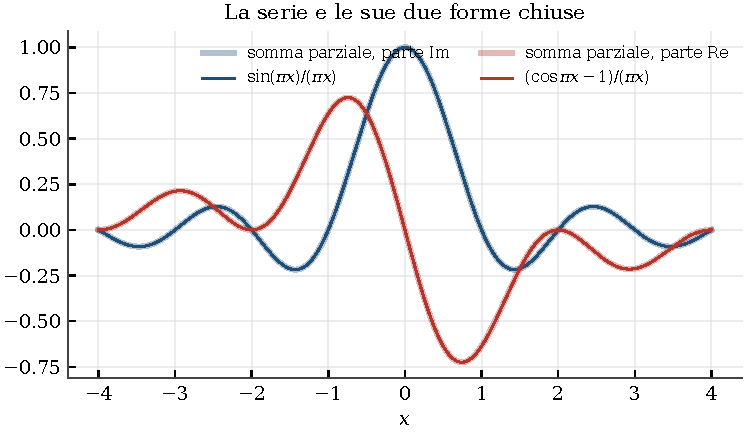
\includegraphics[width=0.86\linewidth]{../figures/cosinc_serie.pdf}
  \caption{La somma parziale della serie della riga $\#14$ (tratto spesso) confrontata con le due forme chiuse delle righe $\#15$ e $\#16$. Quaranta termini bastano a coprire l'intervallo mostrato.}
  \label{fig:cosinc_serie}
\end{figure}
\begin{espr}{17}{User}{}
\[
\frac{1 - \cos\!\left(\pi\, x\right)}{\pi\, x}
\]
\end{espr}
La stessa funzione con il segno cambiato, nella forma che verrà integrata.

\begin{figure}[htbp]
  \centering
  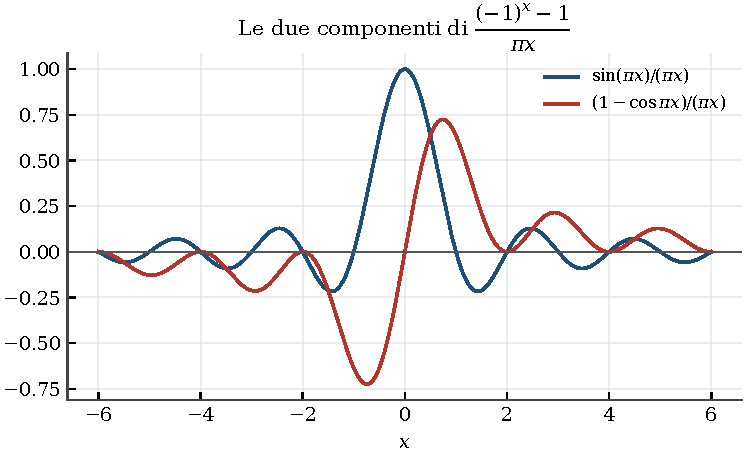
\includegraphics[width=0.86\linewidth]{../figures/sinc_cosinc.pdf}
  \caption{Le due componenti. Entrambe decrescono come $1/x$, ma il seno cardinale cambia segno a ogni intero e le sue aree si compensano, mentre l'altra resta positiva e la sua coda diverge.}
  \label{fig:sinc_cosinc}
\end{figure}

Lo sviluppo è immediato una volta riconosciuto l'esponenziale:
\[
  \frac{\mathrm{e}^{\mathrm{i}\pi x}-1}{\pi x}
  =\frac{1}{\pi x}\sum_{m\ge1}\frac{(\mathrm{i}\pi x)^m}{m!}
  =\sum_{n\ge0}\frac{\mathrm{i}^{\,n+1}(\pi x)^n}{(n+1)!},
\]
che è esattamente il termine generale della riga $\#14$. La parte immaginaria della somma è $\sin(\pi x)/(\pi x)$, cioè il seno cardinale normalizzato; la parte reale è $\left(\cos(\pi x)-1\right)/(\pi x)$. Le righe $\#15$ e $\#16$ affermano proprio questo, e la verifica numerica le conferma.

\section{Due integrali che si comportano in modo opposto}

Qui il quaderno confronta le due componenti sotto integrale su tutta la retta, e trova una differenza radicale. Su una delle due, però, Derive dà una risposta che va guardata con attenzione.

\begin{espr}{18}{User}{}
\[
2\, \int_{0}^{+\infty} \frac{1 - \cos\!\left(\pi\, x\right)}{\pi\, x} \,\mathrm{d}x
\]
\end{espr}
L'integrale su tutta la semiretta positiva, raddoppiato per simmetria.

\begin{espr}{19}{User}{}
\[
\int_{-+\infty}^{+\infty} \frac{\sin\!\left(\pi\, x\right)}{\pi\, x} \,\mathrm{d}x = 1
\]
\end{espr}
L'integrale del seno cardinale: vale esattamente uno. È l'integrale di Dirichlet.

\begin{espr}{20}{User}{}
\[
2\, \int_{0}^{+\infty} \frac{1 - \cos\!\left(\pi\, x\right)}{\pi\, x} \,\mathrm{d}x = 11.53414128
\]
\end{espr}
Il valore restituito per l'altra componente. L'integrale però diverge logaritmicamente: il numero è l'effetto di un troncamento della quadratura numerica intorno a $x\approx10^7$.

\begin{espr}{21}{User}{}
\[
\frac{11.53414128}{2}
\]
\end{espr}
La metà del valore precedente.

\begin{espr}{22}{User}{\verificata}
\[
\frac{11.53414128}{2} = 5.76707064
\]
\end{espr}
Che eredita lo stesso problema.

\begin{espr}{23}{User}{}
\[
\frac{\cos\!\left(\pi\, x\right) - 1}{\pi\, x}
\]
\end{espr}
La componente reale scritta con il segno opposto.

\begin{espr}{24}{User}{}
\[
\int \frac{1 - \cos\!\left(\pi\, x\right)}{\pi\, x} \,\mathrm{d}x
\]
\end{espr}
Il suo integrale indefinito.

\begin{espr}{25}{Int(User,x)}{}
\[
\int \frac{\sin\!\left(\pi\, x\right)}{\pi\, x} \,\mathrm{d}x
\]
\end{espr}
E quello del seno cardinale, che è il seno integrale.


Il seno cardinale è integrabile in senso improprio e la riga $\#19$ dà il valore corretto: $\int_{-\infty}^{+\infty}\frac{\sin\pi x}{\pi x}\,\mathrm{d}x=1$. È l'integrale di Dirichlet, e vale esattamente uno grazie alla normalizzazione con $\pi$.

L'altra componente non è integrabile. Per $x$ grande $\left(1-\cos\pi x\right)/(\pi x)$ oscilla attorno a $1/(\pi x)$, la cui coda diverge logaritmicamente: l'integrale cresce come $\frac{1}{\pi}\ln R$ e non ha limite. Il valore $11{,}53414128$ della riga $\#20$ non è dunque il valore dell'integrale, ma il risultato di una quadratura numerica troncata. Rifacendo il conto si trova che il troncamento corrisponde a un estremo superiore di circa $10^7$: portandolo a $10^9$ il risultato sale a $14{,}4$, e continua a crescere. È il caso in cui un sistema di calcolo restituisce un numero dove non ce n'è uno, e le righe $\#21$ e $\#22$, che ne prendono la metà, ereditano lo stesso problema.

La differenza fra le due componenti non è un dettaglio tecnico: è la ragione per cui il seno cardinale è il nucleo del campionamento e la sua parte reale no.

\section{Derivate e riscritture}

Le ultime righe calcolano la derivata della componente reale e chiudono riscrivendo la funzione di partenza nella forma che ne rende evidente la struttura.

\begin{espr}{26}{User}{}
\[
\frac{\mathrm{d}}{\mathrm{d}x}\!\left[\frac{1 - \cos\!\left(\pi\, x\right)}{\pi\, x}\right]
\]
\end{espr}
Si deriva la componente reale.

\begin{espr}{27}{Simp(\#26)}{}
\[
\frac{\cos\!\left(\pi\, x\right)}{\pi\, x^{2}} + \frac{\sin\!\left(\pi\, x\right)}{x} - \frac{1}{\pi\, x^{2}}
\]
\end{espr}
Il risultato, con i tre termini che si compensano nell'origine.

\begin{espr}{28}{User}{\verificata}
\[
\lim_{h \to 0^{+}} \frac{\left(-1\right)^{h} - 1}{\pi\, h} = \mathrm{i}
\]
\end{espr}
Il limite destro del rapporto incrementale: $\mathrm{i}$, questa volta correttamente.

\begin{espr}{29}{User}{\verificata}
\[
\frac{\left(-1\right)^{x} - 1}{\pi\, x} = \frac{\cos\!\left(\pi\, x\right) - 1 + \mathrm{i}\, \sin\!\left(\pi\, x\right)}{\pi\, x}
\]
\end{espr}
La conclusione: la funzione di partenza scomposta nelle sue due componenti reali.


La riga $\#29$ è la conclusione del quaderno ed è la sua unica affermazione veramente riassuntiva: $\dfrac{(-1)^x-1}{\pi x}=\dfrac{\cos\pi x-1+\mathrm{i}\sin\pi x}{\pi x}$. Tutto il resto è la lettura, componente per componente, di questa uguaglianza.

\section*{In sintesi}
\addcontentsline{toc}{section}{In sintesi}

Il quaderno isola una funzione complessa elementare e ne separa le due parti, scoprendo che si assomigliano in tutto tranne che nella cosa che conta: una ha area finita, l'altra no. È anche il posto in cui la domanda posta sedici mesi prima in \dfw{j.dfw} — si può ottenere $\mathrm{i}$ come limite di un rapporto? — riceve finalmente una risposta affermativa e corretta.


%% generato automaticamente da tools/build_tex.py --- non modificare
\chapter{Oscillazioni a frequenza crescente}
\label{cap:cost2}
\quaderno{cost\textasciicircum{}2.dfw}{24 Jun 2010}{22}

Giugno 2010. Ventidue espressioni su $\cos(t^2)$ e $\sin(t^2)$: funzioni che oscillano sempre più rapidamente man mano che ci si allontana dall'origine, e i cui integrali non si esprimono con funzioni elementari. Sono gli integrali di Fresnel, e il quaderno li incontra senza chiamarli per nome. La sezione finale, però, arriva a un risultato esatto e notevole.

\section{Le funzioni e le loro derivate}

Le prime dodici righe stabiliscono il comportamento sotto derivazione, che è ordinato e prevedibile.

\begin{espr}{1}{User}{}
\[
\sin\!\left(t^{2}\right)
\]
\end{espr}
Il seno di un quadrato: oscilla sempre più rapidamente al crescere di $|t|$.

\begin{espr}{2}{User}{}
\[
\cos\!\left(t^{2}\right)
\]
\end{espr}
Il coseno corrispondente.

\begin{espr}{3}{User}{}
\[
\sin^{2}\!\left(t^{2}\right)
\]
\end{espr}
Il quadrato del primo.

\begin{espr}{4}{User}{}
\[
\cos^{2}\!\left(t^{2}\right)
\]
\end{espr}
E del secondo. La loro somma vale identicamente uno.

\begin{espr}{5}{Dif(\#2,t)}{}
\[
\frac{\mathrm{d}}{\mathrm{d}t}\!\left[\cos\!\left(t^{2}\right)\right]
\]
\end{espr}
Si deriva il coseno.

\begin{espr}{6}{Simp(Dif(\#2,t))}{}
\[
-2\, t\, \sin\!\left(t^{2}\right)
\]
\end{espr}
Il risultato: compare il fattore $2t$, responsabile dell'infittirsi delle oscillazioni.

\begin{espr}{7}{Dif(\#1,t)}{}
\[
\frac{\mathrm{d}}{\mathrm{d}t}\!\left[\sin\!\left(t^{2}\right)\right]
\]
\end{espr}
Si deriva il seno.

\begin{espr}{8}{Simp(Dif(\#1,t))}{}
\[
2\, t\, \cos\!\left(t^{2}\right)
\]
\end{espr}
Con il segno opposto, come atteso.

\begin{espr}{9}{Dif(\#6,t)}{}
\[
\frac{\mathrm{d}}{\mathrm{d}t}\!\left[-2\, t\, \sin\!\left(t^{2}\right)\right]
\]
\end{espr}
Seconda derivata del coseno.

\begin{espr}{10}{Simp(Dif(\#6,t))}{}
\[
-4\, t^{2}\, \cos\!\left(t^{2}\right) - 2\, \sin\!\left(t^{2}\right)
\]
\end{espr}
Compaiono un termine in $t^2$ e uno costante.

\begin{espr}{11}{Dif(\#8,t)}{}
\[
\frac{\mathrm{d}}{\mathrm{d}t}\!\left[2\, t\, \cos\!\left(t^{2}\right)\right]
\]
\end{espr}
Seconda derivata del seno.

\begin{espr}{12}{Simp(Dif(\#8,t))}{}
\[
2\, \cos\!\left(t^{2}\right) - 4\, t^{2}\, \sin\!\left(t^{2}\right)
\]
\end{espr}
La struttura è la stessa, con le funzioni scambiate.


Derivando una volta compare il fattore $2t$, derivando due volte compaiono un termine in $t^2$ e uno costante. Il punto rilevante è che le due funzioni si scambiano a ogni derivazione ma il fattore $2t$ cresce: è questo che rende l'oscillazione sempre più fitta e che impedisce alle primitive di essere elementari.

\section{Le combinazioni e i loro integrali}

Il quaderno costruisce la semisomma e la semidifferenza delle due funzioni e ne chiede le primitive.

\begin{espr}{13}{User}{}
\[
\frac{\cos\!\left(t^{2}\right) + \sin\!\left(t^{2}\right)}{2}
\]
\end{espr}
La semisomma delle due funzioni.

\begin{espr}{14}{Int(\#13,t)}{}
\[
\int \frac{\cos\!\left(t^{2}\right) + \sin\!\left(t^{2}\right)}{2} \,\mathrm{d}t
\]
\end{espr}
Il suo integrale indefinito, che Derive lascia indicato.

\begin{espr}{15}{User}{}
\[
\int \frac{\cos\!\left(t^{2}\right) - \sin\!\left(t^{2}\right)}{2} \,\mathrm{d}t
\]
\end{espr}
La semidifferenza, con lo stesso trattamento.

\begin{espr}{16}{Int(\#2,t)}{}
\[
\int \cos\!\left(t^{2}\right) \,\mathrm{d}t
\]
\end{espr}
L'integrale del solo coseno: è l'integrale di Fresnel $C$.

\begin{espr}{17}{Int(\#1,t)}{}
\[
\int \sin\!\left(t^{2}\right) \,\mathrm{d}t
\]
\end{espr}
E quello del solo seno: l'integrale di Fresnel $S$. Nessuno dei due è elementare.

\begin{figure}[htbp]
  \centering
  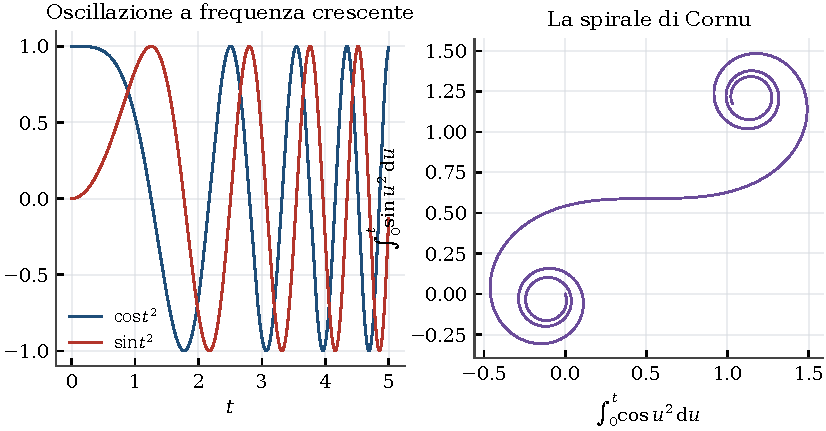
\includegraphics[width=0.86\linewidth]{../figures/fresnel.pdf}
  \caption{A sinistra le due funzioni: l'oscillazione si infittisce come $t$. A destra la curva che ha per coordinate i due integrali di Fresnel — la spirale di Cornu — i cui due punti limite sono le code convergenti dell'integrale improprio.}
  \label{fig:fresnel}
\end{figure}

Derive restituisce gli integrali senza valutarli, e fa bene: non esistono primitive elementari. Le funzioni $\int_0^t\cos u^2\,\mathrm{d}u$ e $\int_0^t\sin u^2\,\mathrm{d}u$ sono per definizione gli integrali di Fresnel, e la curva che si ottiene prendendole come coordinate di un punto è la spirale di Cornu — una delle curve più belle dell'analisi, e quella che descrive la diffrazione della luce da un bordo.

\section{L'integrale improprio}

L'ultima sezione introduce un parametro di frequenza e passa all'integrale su tutta la retta. Qui, dove la primitiva non esisteva, il valore esiste.

\begin{espr}{18}{User}{}
\[
\frac{\cos\!\left(\omega\, t^{2}\right) + \sin\!\left(\omega\, t^{2}\right)}{2}
\]
\end{espr}
Si introduce una frequenza $\omega$.

\begin{espr}{19}{User}{}
\[
\int_{-\infty}^{+\infty} \frac{\cos\!\left(\omega\, t^{2}\right) + \sin\!\left(\omega\, t^{2}\right)}{2} \,\mathrm{d}t
\]
\end{espr}
L'integrale su tutta la retta.

\begin{espr}{20}{Simp(\#19)}{}
\[
\frac{\sqrt{2}\, \sqrt{\pi}}{2\, \sqrt{\omega}}
\]
\end{espr}
Il valore esatto, $\sqrt{\pi/(2\omega)}$: l'integrale converge pur non essendo la funzione infinitesima all'infinito.

\begin{espr}{21}{User}{}
\[
\int_{-\infty}^{+\infty} \frac{t^{2}\, \left(\cos\!\left(\omega\, t^{2}\right) + \sin\!\left(\omega\, t^{2}\right)\right)}{2} \,\mathrm{d}t
\]
\end{espr}
Lo stesso integrale con un fattore $t^2$.

\begin{espr}{22}{Simp(\#21)}{}
\[
2\, \int_{0}^{\infty} \frac{t^{2}\, \cos\!\left(t^{2}\, \omega\right)}{2} + \frac{t^{2}\, \sin\!\left(t^{2}\, \omega\right)}{2} \,\mathrm{d}t
\]
\end{espr}
Derive lo riscrive sfruttando la parità ma non lo valuta: con quel fattore la cancellazione delle oscillazioni non basta più e l'integrale diverge.


Il risultato della riga $\#20$ è esatto e vale la pena di ricostruirlo. Gli integrali di Fresnel su tutta la semiretta valgono
\[
  \int_0^{+\infty}\cos\!\left(\omega t^2\right)\mathrm{d}t
  =\int_0^{+\infty}\sin\!\left(\omega t^2\right)\mathrm{d}t
  =\frac{1}{2}\sqrt{\frac{\pi}{2\omega}},
\]
e su tutta la retta valgono il doppio. La semisomma delle due dà dunque $\sqrt{\pi/(2\omega)}$, che è esattamente $\dfrac{\sqrt2\,\sqrt\pi}{2\sqrt\omega}$ come scritto.

È il fenomeno tipico degli integrali oscillanti: la funzione non tende a zero all'infinito e non è assolutamente integrabile, eppure l'integrale converge, perché le oscillazioni diventano così fitte che i contributi positivi e negativi si cancellano sempre meglio. La riga $\#21$ prova a spingersi oltre inserendo un fattore $t^2$, e lì la cancellazione non basta più: l'integrale diverge, e Derive si limita a riscriverlo sfruttando la parità, senza valutarlo.

\section*{In sintesi}
\addcontentsline{toc}{section}{In sintesi}

Ventidue righe che percorrono la distanza fra due situazioni opposte: una funzione le cui primitive non sono esprimibili con funzioni elementari, e il cui integrale su tutta la retta è invece una radice quadrata di $\pi$ scritta in tre simboli. Fra le due cose sta la spirale di Cornu, che il quaderno non disegna ma che le sue righe descrivono per intero.


%% generato automaticamente da tools/build_tex.py --- non modificare
\chapter{La gaussiana dal cerchio}
\label{cap:gauss}
\quaderno{gauss.dfw}{15 Sep 2010}{14}

Settembre 2010. Quattordici espressioni con un obiettivo dichiarato dal nome del file e mai scritto per esteso: arrivare alla funzione degli errori partendo dalla parametrizzazione razionale del cerchio. Il collegamento fra le due cose esiste ed è semplice — la gaussiana è la formula del cerchio letta sull'asse immaginario — ma il tratto finale, quello che porterebbe a $\operatorname{erf}$, resta aperto.

\section{La parametrizzazione razionale}

La prima riga contiene quattro scritture della stessa cosa, ed è il punto di partenza. Posto $s=\tan(t/2)$, si ha $\mathrm{e}^{\mathrm{i}t}=\dfrac{(1+\mathrm{i}s)^2}{1+s^2}$: è la sostituzione di Weierstrass, quella che rende razionale ogni integrale trigonometrico.

\begin{espr}{1}{User}{}
\begin{align*}
& \mathrm{e}^{\mathrm{i}\, t} \\
=\;& \frac{\left(1 + \mathrm{i}\, \tan\!\left(\frac{t}{2}\right)\right)^{2}}{1 + \tan^{2}\!\left(\frac{t}{2}\right)} \\
=\;& \frac{\left(1 + \mathrm{i}\, \tan\!\left(\frac{t}{2}\right)\right)^{2}}{\left|1 + \mathrm{i}\, \tan\!\left(\frac{t}{2}\right)\right|^{2}} \\
=\;& \operatorname{sgn}^{2}\!\left(1 + \mathrm{i}\, \tan\!\left(\frac{t}{2}\right)\right) \\
=\;& \frac{\cos\!\left(t\right) + 1}{2}\, \left(1 + \mathrm{i}\, \tan\!\left(\frac{t}{2}\right)\right)^{2}
\end{align*}
\end{espr}
Quattro scritture equivalenti dell'esponenziale immaginario, tutte fondate sulla tangente dell'angolo metà.

\begin{espr}{2}{User}{\verificata}
\[
1 + \tan^{2}\!\left(\frac{t}{2}\right) = \frac{2}{\cos\!\left(t\right) + 1}
\]
\end{espr}
L'identità che lega la secante quadra dell'angolo metà al coseno dell'angolo intero.

\begin{espr}{3}{User}{}
\[
\int 1 + \tan^{2}\!\left(\frac{t}{2}\right) \,\mathrm{d}t = 2\, \tan\!\left(\frac{t}{2}\right)
\]
\end{espr}
La stessa quantità è la derivata di $2\tan(t/2)$: l'osservazione serve alla riga seguente.

\begin{espr}{4}{User}{\verificata}
\begin{align*}
& \mathrm{e}^{\mathrm{i}\, t} \\
=\;& \frac{\left(1 + \mathrm{i}\, \tan\!\left(\frac{t}{2}\right)\right)^{2}}{\frac{\mathrm{d}}{\mathrm{d}t}\!\left[2\, \tan\!\left(\frac{t}{2}\right)\right]}
\end{align*}
\end{espr}
L'esponenziale scritto come rapporto fra un quadrato e una derivata.


La verifica è diretta: $(1+\mathrm{i}s)^2=1-s^2+2\mathrm{i}s$, e dividendo per $1+s^2$ si ottengono esattamente $\cos t$ e $\sin t$ in funzione della tangente dell'angolo metà. La riga $\#2$ registra l'identità $1+\tan^2(t/2)=2/(1+\cos t)$ e la riga $\#3$ osserva che quella stessa quantità è la derivata di $2\tan(t/2)$. La riga $\#4$ ne trae la scrittura più suggestiva: l'esponenziale immaginario è un quadrato diviso per una derivata.

\section{Il passaggio all'argomento immaginario}

Una riga sola, ed è il centro del quaderno.

\begin{espr}{5}{Sub(User)}{\verificata}
\begin{align*}
& \mathrm{e}^{\mathrm{i}\, \left(\mathrm{i}\, x^{2}\right)} \\
=\;& \frac{\left(1 + \mathrm{i}\, \tan\!\left(\frac{\mathrm{i}\, x^{2}}{2}\right)\right)^{2}}{1 + \tan^{2}\!\left(\frac{\mathrm{i}\, x^{2}}{2}\right)} \\
=\;& \frac{\cos\!\left(\mathrm{i}\, x^{2}\right) + 1}{2}\, \left(1 + \mathrm{i}\, \tan\!\left(\frac{\mathrm{i}\, x^{2}}{2}\right)\right)^{2}
\end{align*}
\end{espr}
La riga centrale: con $t=\mathrm{i}x^2$ il primo membro è la gaussiana, e il secondo si riduce a $\left(\cosh-\sinh\right)^2$.


Sostituendo $t=\mathrm{i}x^2$ il primo membro diventa $\mathrm{e}^{\mathrm{i}\cdot\mathrm{i}x^2}=\mathrm{e}^{-x^2}$: la gaussiana. E il secondo membro si semplifica altrettanto bene. Poiché $\tan(\mathrm{i}u)=\mathrm{i}\tanh u$, si ha $1+\mathrm{i}\tan\!\left(\mathrm{i}\tfrac{x^2}{2}\right)=1-\tanh\tfrac{x^2}{2}$ e $1+\tan^2\!\left(\mathrm{i}\tfrac{x^2}{2}\right)=\operatorname{sech}^2\tfrac{x^2}{2}$, per cui il rapporto vale
\[
  \left(1-\tanh\tfrac{x^2}{2}\right)^2\cosh^2\tfrac{x^2}{2}
  =\left(\cosh\tfrac{x^2}{2}-\sinh\tfrac{x^2}{2}\right)^2
  =\mathrm{e}^{-x^2}.
\]
La gaussiana è dunque, letteralmente, la stessa formula che parametrizza il cerchio, letta lungo l'asse immaginario. È il risultato per cui il quaderno esiste.

\section{L'integrale della funzione segno}

Il tentativo di chiudere il cerchio parte da un'osservazione elementare e passa per un integrale che Derive risolve in una forma inaspettata.

\begin{espr}{6}{User}{}
\[
\int \operatorname{sgn}\!\left(x\right) \,\mathrm{d}x = \left|x\right|
\]
\end{espr}
Il modello da imitare: la primitiva del segno è il valore assoluto.

\begin{espr}{7}{User}{}
\[
\operatorname{sgn}\!\left(1 + \mathrm{i}\, \tan\!\left(\frac{t}{2}\right)\right)
\]
\end{espr}
La funzione segno del numero che parametrizza il cerchio: ha modulo uno ma è discontinua.

\begin{espr}{8}{Int(\#7,t)}{}
\[
\int \operatorname{sgn}\!\left(1 + \mathrm{i}\, \tan\!\left(\frac{t}{2}\right)\right) \,\mathrm{d}t
\]
\end{espr}
Se ne chiede la primitiva.

\begin{espr}{9}{Simp(Int(\#7,t))}{}
\[
-4\, \left\lfloor \frac{1}{2} - \frac{t}{2\, \pi} \right\rfloor + \frac{\sqrt{2}\, \sin\!\left(t\right)}{\sqrt{\cos\!\left(t\right) + 1}} - \sqrt{2}\, \mathrm{i}\, \sqrt{\cos\!\left(t\right) + 1}
\]
\end{espr}
La risposta. Il termine con la parte intera raccorda i tratti fra un salto e il successivo.

\begin{figure}[htbp]
  \centering
  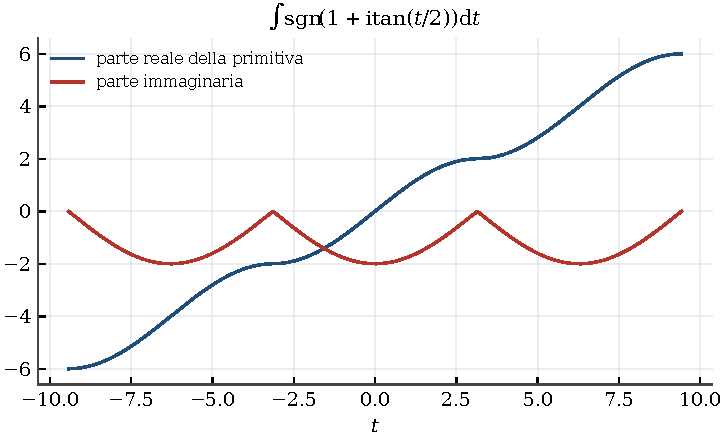
\includegraphics[width=0.86\linewidth]{../figures/gauss_sign.pdf}
  \caption{La primitiva della riga $\#9$. La parte reale sale a gradini raccordati — è l'effetto del termine con la parte intera — mentre la parte immaginaria è periodica e vale $-2\left|\cos(t/2)\right|$.}
  \label{fig:gauss_sign}
\end{figure}
\begin{espr}{10}{User}{}
\[
-4\, \left\lfloor \frac{1}{2} - \frac{t}{2\, \pi} \right\rfloor + \frac{\sqrt{2}\, \sin\!\left(t\right)}{\sqrt{\cos\!\left(t\right) + 1}}
\]
\end{espr}
La sola parte reale della primitiva.

\begin{espr}{11}{User}{}
\[
\operatorname{erf}\!\left(t\right)
\]
\end{espr}
La funzione degli errori, scritta da sola: è l'obiettivo verso cui il quaderno si sta muovendo.


La riga $\#6$ ricorda che la primitiva della funzione segno è il valore assoluto: è il modello di quello che si vorrebbe ottenere, una funzione non elementare come primitiva di una elementare a tratti.

La riga $\#9$ è la risposta di Derive all'integrale della riga $\#8$, e il termine con la parte intera merita una spiegazione. La quantità $\mathrm{sgn}\!\left(1+\mathrm{i}\tan\tfrac{t}{2}\right)$ ha modulo uno, e verrebbe da scrivere che vale $\mathrm{e}^{\mathrm{i}t/2}$ — ma non è così, perché il numero $1+\mathrm{i}\tan(t/2)$ ha sempre parte reale uguale a $1$ e quindi argomento confinato fra $-\pi/2$ e $\pi/2$. La funzione è discontinua, salta di $\pi$ ogni volta che la tangente diverge, e la primitiva deve rimettere insieme i tratti: è questo il compito del termine $-4\left\lfloor\tfrac12-\tfrac{t}{2\pi}\right\rfloor$, che aggiunge una costante diversa su ogni periodo. Le due parti restanti, riscritte con $\cos t+1=2\cos^2(t/2)$, valgono $2\sin\tfrac t2\,\mathrm{sgn}\!\left(\cos\tfrac t2\right)$ e $-2\mathrm{i}\left|\cos\tfrac t2\right|$.

\section{Il tratto che resta aperto}

Le ultime tre righe applicano al caso quadratico la stessa costruzione e si fermano lì.

\begin{espr}{12}{User}{}
\[
\int \operatorname{sgn}\!\left(1 + \mathrm{i}\, \tan\!\left(\frac{t^{2}}{2}\right)\right) \,\mathrm{d}t
\]
\end{espr}
La stessa costruzione con argomento quadratico.

\begin{espr}{13}{Simp(User)}{}
\[
\frac{\sqrt{2}\, \int \sqrt{\cos\!\left(t^{2}\right) + 1} \,\mathrm{d}t}{2} + \frac{\sqrt{2}\, \mathrm{i}\, \int \frac{\sin\!\left(t^{2}\right)}{\sqrt{\cos\!\left(t^{2}\right) + 1}} \,\mathrm{d}t}{2}
\]
\end{espr}
Che si spezza in due integrali di tipo Fresnel, nessuno dei quali elementare.

\begin{espr}{14}{User}{}
\[
\int \operatorname{sgn}\!\left(1 + \mathrm{i}\, \tan\!\left(\frac{\mathrm{i}\, t^{2}}{2}\right)\right) \,\mathrm{d}t
\]
\end{espr}
Il tentativo con argomento immaginario, lasciato senza risposta. Qui la funzione segno vale identicamente uno e la costruzione si svuota.


Sostituendo $t\to t^2$, l'integrale si spezza nelle due parti della riga $\#13$, che sono integrali di tipo Fresnel: la stessa famiglia incontrata tre mesi prima in \dfw{cost\\textasciicircum{}{}2.dfw} (capitolo~\ref{cap:cost2}). La riga $\#14$ tenta il passaggio all'argomento immaginario, quello che secondo la riga $\#5$ dovrebbe produrre la gaussiana e quindi, integrando, la funzione degli errori. Derive non porta a termine il calcolo e il quaderno si interrompe.

Vale la pena notare che il passaggio non è solo un problema di software. Con argomento immaginario la quantità $1+\mathrm{i}\tan\!\left(\mathrm{i}t^2/2\right)=1-\tanh(t^2/2)$ è reale e positiva, quindi la sua funzione segno vale identicamente uno e l'integrale è banalmente $t$: la costruzione perde per strada proprio l'informazione che serviva. Per ottenere $\operatorname{erf}$ occorre integrare la gaussiana, non il segno di ciò che la genera.

\section*{In sintesi}
\addcontentsline{toc}{section}{In sintesi}

Il risultato del quaderno è che la gaussiana è la parametrizzazione razionale del cerchio valutata lungo l'asse immaginario: $\mathrm{e}^{-x^2}=\left(1-\tanh\tfrac{x^2}{2}\right)/\left(1+\tanh\tfrac{x^2}{2}\right)$. Preso da solo è un'osservazione semplice; è però un pezzo di un'idea che attraversa cinque quaderni, l'esponenziale scritto con la tangente del semiangolo, che la nota a corredo di questa edizione ricostruisce per intero. Il programma che l'autore si era dato — arrivare da lì alla funzione degli errori — non viene completato, e la ragione non è la debolezza del calcolatore ma la struttura del problema: la funzione segno, che nel caso circolare portava l'informazione utile, nel caso immaginario diventa costante.


%% generato automaticamente da tools/build_tex.py --- non modificare
\chapter{Una delta di Dirac che vive nel piano complesso}
\label{cap:delta}
\quaderno{delta.dfw}{13 Jul 2010}{55}

Luglio 2010, cinquantacinque espressioni. È il quaderno più ambizioso della raccolta. Si parte da una famiglia di funzioni elementari che approssima la delta di Dirac; si osserva che la formula, scritta com'è, ha senso anche per argomento complesso; e si studia la funzione che ne risulta. Il finale tenta di usare quella funzione per dare un valore alla trasformata di Fourier di un esponenziale crescente, che nel senso ordinario non esiste. I conti sono corretti; come si vedrà, però, il valore ottenuto dipende dalla famiglia approssimante scelta, e non dalla delta.

\section{La famiglia approssimante}

Tutto il quaderno si regge su questa espressione, ripetuta decine di volte con argomenti sempre diversi. Conviene capirla subito, perché è molto più semplice di quanto sembri.

\begin{espr}{1}{Lim(User,n)}{}
\[
\lim_{n \to +\infty} \frac{1}{4}\, \left(\frac{1 + 2\, n\, x}{\left|x + \frac{1}{2\, n}\right|} + \frac{1 - 2\, n\, x}{\left|x - \frac{1}{2\, n}\right|}\right)
\]
\end{espr}
La famiglia approssimante: per ogni $n$ è un rettangolo alto $n$ e largo $1/n$, scritto senza usare definizioni a tratti.

\begin{figure}[htbp]
  \centering
  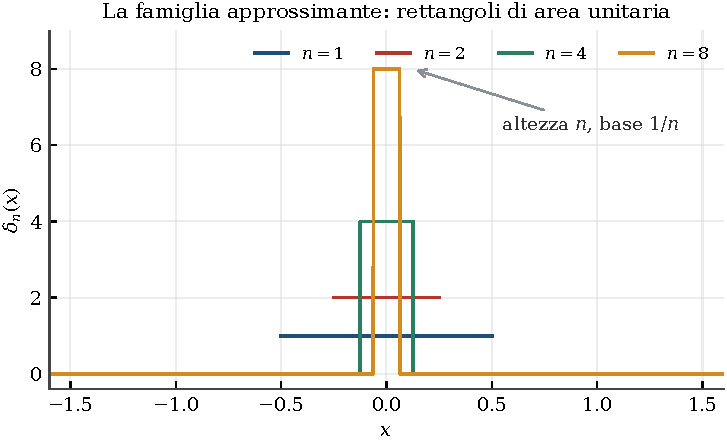
\includegraphics[width=0.86\linewidth]{../figures/delta_famiglia.pdf}
  \caption{La famiglia della riga $\#1$ per quattro valori di $n$. La formula, che non contiene definizioni a tratti, produce esattamente un rettangolo alto $n$ e largo $1/n$.}
  \label{fig:delta_famiglia}
\end{figure}
\begin{espr}{2}{User}{}
\begin{align*}
& \lim_{n \to +\infty} \int_{-\infty}^{+\infty} \frac{1}{4}\, \left(\frac{1 + 2\, n\, x}{\left|x + \frac{1}{2\, n}\right|} + \frac{1 - 2\, n\, x}{\left|x - \frac{1}{2\, n}\right|}\right) \,\mathrm{d}x \\
=\;& 1
\end{align*}
\end{espr}
L'area vale uno per ogni $n$, e quindi anche al limite.

\begin{figure}[htbp]
  \centering
  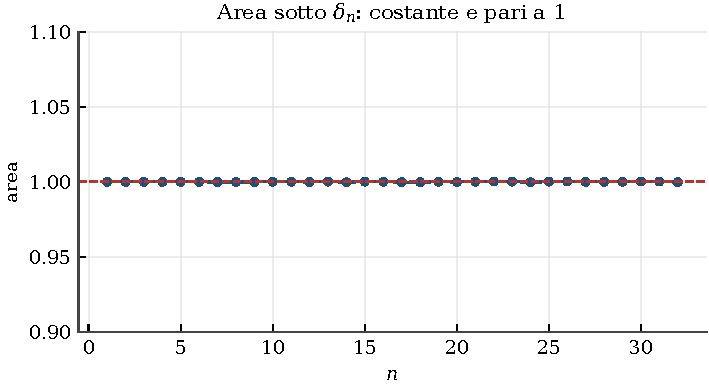
\includegraphics[width=0.86\linewidth]{../figures/delta_area.pdf}
  \caption{Verifica numerica della riga $\#2$: l'area resta uno al crescere di $n$, come deve essere per una famiglia che approssima la delta.}
  \label{fig:delta_area}
\end{figure}
\begin{espr}{3}{User}{}
\begin{align*}
& \lim_{n \to +\infty} \int_{-\infty}^{+\infty} \frac{1}{4}\, \left(\frac{1 + 2\, n\, \left(x - k\right)}{\left|x - k + \frac{1}{2\, n}\right|} + \frac{1 - 2\, n\, \left(x - k\right)}{\left|x - k - \frac{1}{2\, n}\right|}\right) \,\mathrm{d}x \\
=\;& 1
\end{align*}
\end{espr}
La stessa famiglia traslata nel punto $k$: l'area non cambia.


Per $x$ reale il calcolo si fa a mano. Se $|x|>1/(2n)$ i due valori assoluti si aprono con lo stesso segno e i due addendi valgono $+2n$ e $-2n$: la somma è nulla. Se invece $|x|<1/(2n)$ il secondo valore assoluto cambia segno e i due addendi valgono entrambi $2n$: la somma è $4n$, che diviso quattro dà $n$. Dunque
\[
  \delta_n(x)=\begin{cases} n & |x|<\dfrac{1}{2n}\\[6pt] 0 & \text{altrove,}\end{cases}
\]
cioè un rettangolo alto $n$ e largo $1/n$, di area unitaria per costruzione. È l'approssimante più semplice possibile della delta di Dirac, scritta però senza usare né la funzione segno né una definizione a tratti: solo valori assoluti e quozienti. La riga $\#2$ verifica l'area e la riga $\#3$ la trasla nel punto $k$.

\section{Che cosa succede con argomento complesso}

Qui comincia la parte originale. La formula della riga $\#1$ non contiene nulla che richieda un argomento reale: i valori assoluti si leggono come moduli, e tutto il resto è aritmetica. Che funzione si ottiene?

\begin{espr}{4}{User}{\verificata}
\begin{align*}
& \lim_{n \to +\infty} \frac{1}{4}\, \left(\frac{1 + 2\, n\, z}{\left|z + \frac{1}{2\, n}\right|} + \frac{1 - 2\, n\, z}{\left|z - \frac{1}{2\, n}\right|}\right) \\
=\;& \frac{z}{2\, \mathrm{i}\, \left|z\right|^{3}}\, \operatorname{Im}\!\left(z\right)
\end{align*}
\end{espr}
La formula centrale del quaderno. Con argomento complesso il limite non è una distribuzione ma una funzione ordinaria, definita ovunque tranne che nell'origine.

\begin{figure}[htbp]
  \centering
  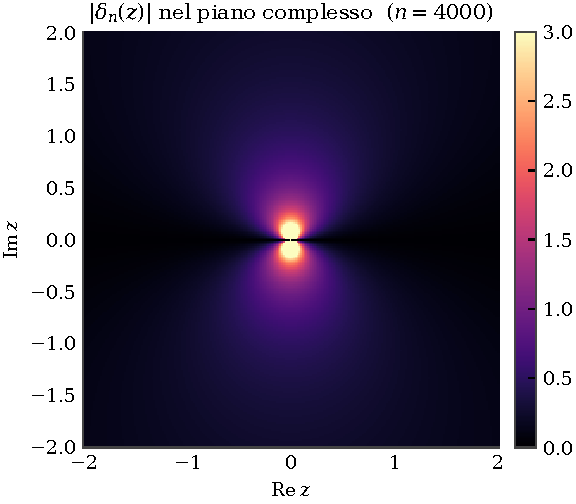
\includegraphics[width=0.62\linewidth]{../figures/delta_complesso.pdf}
  \caption{Il modulo della funzione della riga $\#4$ nel piano complesso. La linea scura lungo l'asse reale è il luogo $\operatorname{Im}z=0$, dove la funzione si annulla; i due lobi chiari sopra e sotto l'origine sono la singolarità $1/|z|$.}
  \label{fig:delta_complesso}
\end{figure}
\begin{espr}{5}{User}{\verificata}
\begin{align*}
& \lim_{n \to +\infty} \frac{1}{4}\, \left(\frac{1 + 2\, n\, \left(\mathrm{i}\, z\right)}{\left|\mathrm{i}\, z + \frac{1}{2\, n}\right|} + \frac{1 - 2\, n\, \left(\mathrm{i}\, z\right)}{\left|\mathrm{i}\, z - \frac{1}{2\, n}\right|}\right) \\
=\;& \frac{z}{2\, \left|z\right|^{3}}\, \operatorname{Re}\!\left(z\right)
\end{align*}
\end{espr}
Ruotando l'argomento di un quarto di giro, $\operatorname{Im}$ diventa $\operatorname{Re}$ e sparisce il fattore $\mathrm{i}$.

\begin{espr}{6}{User}{\verificata}
\begin{align*}
& \lim_{n \to +\infty} \frac{1}{4}\, \left(\frac{1 + 2\, n\, \left(\mathrm{i}\, z\right)}{\left|\mathrm{i}\, z + \frac{1}{2\, n}\right|} + \frac{1 - 2\, n\, \left(\mathrm{i}\, z\right)}{\left|\mathrm{i}\, z - \frac{1}{2\, n}\right|}\right) \\
&\qquad + \lim_{n \to +\infty} \frac{1}{4}\, \left(\frac{1 + 2\, n\, z}{\left|z + \frac{1}{2\, n}\right|} + \frac{1 - 2\, n\, z}{\left|z - \frac{1}{2\, n}\right|}\right) \\
=\;& \frac{1}{2\, \left|z\right|}
\end{align*}
\end{espr}
La somma delle due vale $1/(2|z|)$: si riconosce $z\bar z=|z|^2$.

\begin{espr}{7}{User}{\verificata}
\begin{align*}
& \lim_{n \to +\infty} \frac{1}{4}\, \left(\frac{1 + 2\, n\, \left(\mathrm{i}\, z\right)}{\left|\mathrm{i}\, z + \frac{1}{2\, n}\right|} + \frac{1 - 2\, n\, \left(\mathrm{i}\, z\right)}{\left|\mathrm{i}\, z - \frac{1}{2\, n}\right|}\right) \\
&\qquad - \lim_{n \to +\infty} \frac{1}{4}\, \left(\frac{1 + 2\, n\, z}{\left|z + \frac{1}{2\, n}\right|} + \frac{1 - 2\, n\, z}{\left|z - \frac{1}{2\, n}\right|}\right) \\
=\;& \frac{z^{2}}{2\, \left|z\right|^{3}}
\end{align*}
\end{espr}
La differenza vale $z^2/\left(2|z|^3\right)$.


La risposta della riga $\#4$ è la formula chiave di tutto il quaderno:
\[
  \delta(z)=\lim_{n\to\infty}\delta_n(z)=\frac{z\,\operatorname{Im}z}{2\mathrm{i}\,|z|^{3}}.
\]
Non è più un rettangolo: è una funzione definita su tutto il piano, che si annulla su tutto l'asse reale tranne che nell'origine — dove $\operatorname{Im}z=0$ — e che diverge come $1/|z|$ avvicinandosi all'origine dall'alto o dal basso. Il grafico del modulo ha la forma di un dipolo, con due lobi sopra e sotto lo zero e una linea di annullamento lungo i reali.

Le righe $\#5$--$\#7$ sono la parte che rende il tutto solido, e sono identità esatte. Ruotando l'argomento di un quarto di giro si ottiene la stessa formula con $\operatorname{Re}$ al posto di $\operatorname{Im}$ e senza il fattore $\mathrm{i}$; sommando le due si ottiene
\[
  \delta(\mathrm{i}z)+\delta(z)=\frac{z\left(\operatorname{Re}z-\mathrm{i}\operatorname{Im}z\right)}{2|z|^{3}}=\frac{z\bar z}{2|z|^{3}}=\frac{1}{2|z|},
\]
e sottraendole $\dfrac{z^2}{2|z|^{3}}$. Due righe, e la somma di due oggetti singolari diventa una funzione elementare del solo modulo.

\section{Come si comporta sotto riscalamento}

Le quattordici espressioni seguenti provano la formula su argomenti riscalati: per un fattore trigonometrico, per un fattore iperbolico, per un esponenziale immaginario. Tutte, lette con $\omega$ reale, sono esatte.

\begin{espr}{8}{User}{}
\begin{align*}
& \lim_{n \to +\infty} \frac{1}{4}\, \left(\frac{1 + 2\, n\, \left(z\, \cos\!\left(\omega\right)\right)}{\left|z\, \cos\!\left(\omega\right) + \frac{1}{2\, n}\right|} + \frac{1 - 2\, n\, \left(z\, \cos\!\left(\omega\right)\right)}{\left|z\, \cos\!\left(\omega\right) - \frac{1}{2\, n}\right|}\right) \\
=\;& \frac{\operatorname{Im}\!\left(z\right)\, z}{2\, \mathrm{i}\, \left|z\right|^{3}\, \left|\cos\!\left(\omega\right)\right|}
\end{align*}
\end{espr}
Riscalamento per $\cos\omega$: compare il fattore $1/|\cos\omega|$, esattamente come per la delta ordinaria.

\begin{espr}{9}{User}{}
\begin{align*}
& \lim_{n \to +\infty} \frac{1}{4}\, \left(\frac{1 + 2\, n\, \left(z\, \sin\!\left(\omega\right)\right)}{\left|z\, \sin\!\left(\omega\right) + \frac{1}{2\, n}\right|} + \frac{1 - 2\, n\, \left(z\, \sin\!\left(\omega\right)\right)}{\left|z\, \sin\!\left(\omega\right) - \frac{1}{2\, n}\right|}\right) \\
=\;& \frac{\operatorname{Im}\!\left(z\right)\, z}{2\, \mathrm{i}\, \left|z\right|^{3}\, \left|\sin\!\left(\omega\right)\right|}
\end{align*}
\end{espr}
Riscalamento per $\sin\omega$.

\begin{espr}{10}{User}{}
\begin{align*}
& \lim_{n \to +\infty} \frac{1}{4}\, \left(\frac{1 + 2\, n\, \left(z\, \cos\!\left(\mathrm{i}\, \omega\right)\right)}{\left|z\, \cos\!\left(\mathrm{i}\, \omega\right) + \frac{1}{2\, n}\right|} + \frac{1 - 2\, n\, \left(z\, \cos\!\left(\mathrm{i}\, \omega\right)\right)}{\left|z\, \cos\!\left(\mathrm{i}\, \omega\right) - \frac{1}{2\, n}\right|}\right) \\
=\;& \frac{\operatorname{Im}\!\left(z\right)\, \mathrm{e}^{\omega}\, z}{\mathrm{i}\, \left|z\right|^{3}\, \left(\mathrm{e}^{2\, \omega} + 1\right)}
\end{align*}
\end{espr}
Riscalamento per $\cos(\mathrm{i}\omega)=\cosh\omega$, scritto in forma esponenziale.

\begin{espr}{11}{User}{}
\begin{align*}
& \lim_{n \to +\infty} \frac{1}{4}\, \left(\frac{1 + 2\, n\, \left(z\, \sin\!\left(\mathrm{i}\, \omega\right)\right)}{\left|z\, \sin\!\left(\mathrm{i}\, \omega\right) + \frac{1}{2\, n}\right|} + \frac{1 - 2\, n\, \left(z\, \sin\!\left(\mathrm{i}\, \omega\right)\right)}{\left|z\, \sin\!\left(\mathrm{i}\, \omega\right) - \frac{1}{2\, n}\right|}\right) \\
=\;& \frac{\operatorname{Re}\!\left(z\right)\, \mathrm{e}^{\omega}\, z}{\left|z\right|^{3}\, \left|\mathrm{e}^{2\, \omega} - 1\right|}
\end{align*}
\end{espr}
Riscalamento per $\sin(\mathrm{i}\omega)=\mathrm{i}\sinh\omega$; il fattore $\mathrm{i}$ scambia $\operatorname{Im}$ con $\operatorname{Re}$.

\begin{espr}{12}{User}{\verificata}
\begin{align*}
& \lim_{n \to +\infty} \frac{1}{4}\, \left(\frac{1 + 2\, n\, \mathrm{e}^{\mathrm{i}\, z}}{\left|\mathrm{e}^{\mathrm{i}\, z} + \frac{1}{2\, n}\right|} + \frac{1 - 2\, n\, \mathrm{e}^{\mathrm{i}\, z}}{\left|\mathrm{e}^{\mathrm{i}\, z} - \frac{1}{2\, n}\right|}\right) \\
=\;& \frac{1}{2\, \mathrm{i}}\, \mathrm{e}^{\mathrm{i}\, \left(\operatorname{Re}\!\left(z\right) - \mathrm{i}\, \operatorname{Im}\!\left(z\right)\right)}\, \sin\!\left(\operatorname{Re}\!\left(z\right)\right)
\end{align*}
\end{espr}
Argomento sul cerchio unitario complesso.

\begin{espr}{13}{User}{}
\begin{align*}
& \lim_{n \to +\infty} \frac{1}{4}\, \left(\frac{1 + 2\, n\, \left(\mathrm{i}\, a\, \mathrm{e}^{\mathrm{i}\, z}\right)}{\left|\mathrm{i}\, a\, \mathrm{e}^{\mathrm{i}\, z} + \frac{1}{2\, n}\right|} + \frac{1 - 2\, n\, \left(\mathrm{i}\, a\, \mathrm{e}^{\mathrm{i}\, z}\right)}{\left|\mathrm{i}\, a\, \mathrm{e}^{\mathrm{i}\, z} - \frac{1}{2\, n}\right|}\right) \\
=\;& \frac{\mathrm{e}^{\mathrm{i}\, \left(\operatorname{Re}\!\left(z\right) - \mathrm{i}\, \operatorname{Im}\!\left(z\right)\right)}\, \cos\!\left(\operatorname{Re}\!\left(z\right)\right)}{2\, \left|a\right|}
\end{align*}
\end{espr}
Con un fattore $\mathrm{i}a$ davanti: compare $\cos$ al posto di $\sin$ e il modulo $|a|$ al denominatore.

\begin{espr}{14}{User}{}
\begin{align*}
& \lim_{n \to +\infty} \frac{1}{4}\, \left(\frac{1 + 2\, n\, \left(\mathrm{i}\, a\, \mathrm{e}^{\mathrm{i}\, z}\right)}{\left|\mathrm{i}\, a\, \mathrm{e}^{\mathrm{i}\, z} + \frac{1}{2\, n}\right|} + \frac{1 - 2\, n\, \left(\mathrm{i}\, a\, \mathrm{e}^{\mathrm{i}\, z}\right)}{\left|\mathrm{i}\, a\, \mathrm{e}^{\mathrm{i}\, z} - \frac{1}{2\, n}\right|}\right) \\
&\qquad + \lim_{n \to +\infty} \frac{1}{4}\, \left(\frac{1 + 2\, n\, \left(a\, \mathrm{e}^{\mathrm{i}\, z}\right)}{\left|a\, \mathrm{e}^{\mathrm{i}\, z} + \frac{1}{2\, n}\right|} + \frac{1 - 2\, n\, \left(a\, \mathrm{e}^{\mathrm{i}\, z}\right)}{\left|a\, \mathrm{e}^{\mathrm{i}\, z} - \frac{1}{2\, n}\right|}\right) \\
=\;& \frac{1}{2\, \left|a\right|}\, \mathrm{e}^{-\mathrm{i}\, \operatorname{Im}\!\left(z\right)}
\end{align*}
\end{espr}
La somma delle due versioni con e senza il fattore $\mathrm{i}$.

\begin{espr}{15}{User}{}
\begin{align*}
& \lim_{n \to +\infty} \frac{1}{4}\, \left(\frac{1 + 2\, n\, \left(\mathrm{i}\, a\, \mathrm{e}^{\mathrm{i}\, z}\right)}{\left|\mathrm{i}\, a\, \mathrm{e}^{\mathrm{i}\, z} + \frac{1}{2\, n}\right|} + \frac{1 - 2\, n\, \left(\mathrm{i}\, a\, \mathrm{e}^{\mathrm{i}\, z}\right)}{\left|\mathrm{i}\, a\, \mathrm{e}^{\mathrm{i}\, z} - \frac{1}{2\, n}\right|}\right) \\
&\qquad - \lim_{n \to +\infty} \frac{1}{4}\, \left(\frac{1 + 2\, n\, \left(a\, \mathrm{e}^{\mathrm{i}\, z}\right)}{\left|a\, \mathrm{e}^{\mathrm{i}\, z} + \frac{1}{2\, n}\right|} + \frac{1 - 2\, n\, \left(a\, \mathrm{e}^{\mathrm{i}\, z}\right)}{\left|a\, \mathrm{e}^{\mathrm{i}\, z} - \frac{1}{2\, n}\right|}\right) \\
=\;& \frac{1}{2\, \left|a\right|}\, \mathrm{e}^{\mathrm{i}\, 2\, \operatorname{Re}\!\left(z\right) + \operatorname{Im}\!\left(z\right)}
\end{align*}
\end{espr}
E la loro differenza.

\begin{espr}{16}{User}{}
\begin{align*}
& \lim_{n \to +\infty} \frac{1}{4}\, \left(\frac{1 + 2\, n\, \left(\mathrm{i}\, \mathrm{e}^{\mathrm{i}\, x}\right)}{\left|\mathrm{i}\, \mathrm{e}^{\mathrm{i}\, x} + \frac{1}{2\, n}\right|} + \frac{1 - 2\, n\, \left(\mathrm{i}\, \mathrm{e}^{\mathrm{i}\, x}\right)}{\left|\mathrm{i}\, \mathrm{e}^{\mathrm{i}\, x} - \frac{1}{2\, n}\right|}\right) \\
&\qquad + \lim_{n \to +\infty} \frac{1}{4}\, \left(\frac{1 + 2\, n\, \mathrm{e}^{\mathrm{i}\, x}}{\left|\mathrm{e}^{\mathrm{i}\, x} + \frac{1}{2\, n}\right|} + \frac{1 - 2\, n\, \mathrm{e}^{\mathrm{i}\, x}}{\left|\mathrm{e}^{\mathrm{i}\, x} - \frac{1}{2\, n}\right|}\right) \\
=\;& \frac{1}{2}
\end{align*}
\end{espr}
Il caso particolare $a=1$ con argomento reale: la somma vale $1/2$.

\begin{espr}{17}{User}{}
\begin{align*}
& \lim_{n \to +\infty} \frac{1}{4}\, \left(\frac{1 + 2\, n\, \left(\mathrm{i}\, \mathrm{e}^{\mathrm{i}\, \left(\frac{x}{2}\right)}\right)}{\left|\mathrm{i}\, \mathrm{e}^{\mathrm{i}\, \left(\frac{x}{2}\right)} + \frac{1}{2\, n}\right|} + \frac{1 - 2\, n\, \left(\mathrm{i}\, \mathrm{e}^{\mathrm{i}\, \left(\frac{x}{2}\right)}\right)}{\left|\mathrm{i}\, \mathrm{e}^{\mathrm{i}\, \left(\frac{x}{2}\right)} - \frac{1}{2\, n}\right|}\right) \\
&\qquad - \lim_{n \to +\infty} \frac{1}{4}\, \left(\frac{1 + 2\, n\, \mathrm{e}^{\mathrm{i}\, \left(\frac{x}{2}\right)}}{\left|\mathrm{e}^{\mathrm{i}\, \left(\frac{x}{2}\right)} + \frac{1}{2\, n}\right|} + \frac{1 - 2\, n\, \mathrm{e}^{\mathrm{i}\, \left(\frac{x}{2}\right)}}{\left|\mathrm{e}^{\mathrm{i}\, \left(\frac{x}{2}\right)} - \frac{1}{2\, n}\right|}\right) \\
=\;& \frac{1}{2}\, \mathrm{e}^{\mathrm{i}\, x}
\end{align*}
\end{espr}
Con argomento dimezzato: la differenza ricostruisce $\mathrm{e}^{\mathrm{i}x}/2$.

\begin{espr}{18}{User}{}
\begin{align*}
& \lim_{n \to +\infty} \frac{1}{4}\, \left(\frac{1 + 2\, n\, \mathrm{e}^{\mathrm{i}\, z}}{\left|\mathrm{e}^{\mathrm{i}\, z} + \frac{1}{2\, n}\right|} + \frac{1 - 2\, n\, \mathrm{e}^{\mathrm{i}\, z}}{\left|\mathrm{e}^{\mathrm{i}\, z} - \frac{1}{2\, n}\right|}\right) \\
&\qquad + \lim_{n \to +\infty} \frac{1}{4}\, \left(\frac{1 + 2\, n\, \mathrm{e}^{-\mathrm{i}\, z}}{\left|\mathrm{e}^{-\mathrm{i}\, z} + \frac{1}{2\, n}\right|} + \frac{1 - 2\, n\, \mathrm{e}^{-\mathrm{i}\, z}}{\left|\mathrm{e}^{-\mathrm{i}\, z} - \frac{1}{2\, n}\right|}\right) \\
=\;& \sin^{2}\!\left(z\right)
\end{align*}
\end{espr}
Somma delle versioni con esponenti coniugati: dà $\sin^2 z$.

\begin{espr}{19}{User}{}
\begin{align*}
& \lim_{n \to +\infty} \frac{1}{4}\, \left(\frac{1 + 2\, n\, \mathrm{e}^{\mathrm{i}\, z}}{\left|\mathrm{e}^{\mathrm{i}\, z} + \frac{1}{2\, n}\right|} + \frac{1 - 2\, n\, \mathrm{e}^{\mathrm{i}\, z}}{\left|\mathrm{e}^{\mathrm{i}\, z} - \frac{1}{2\, n}\right|}\right) \\
&\qquad - \lim_{n \to +\infty} \frac{1}{4}\, \left(\frac{1 + 2\, n\, \mathrm{e}^{-\mathrm{i}\, z}}{\left|\mathrm{e}^{-\mathrm{i}\, z} + \frac{1}{2\, n}\right|} + \frac{1 - 2\, n\, \mathrm{e}^{-\mathrm{i}\, z}}{\left|\mathrm{e}^{-\mathrm{i}\, z} - \frac{1}{2\, n}\right|}\right) \\
=\;& -\mathrm{i}\, \sin\!\left(z\right)\, \cos\!\left(z\right)
\end{align*}
\end{espr}
La differenza dà $-\mathrm{i}\sin z\cos z$, cioè metà del seno dell'angolo doppio.

\begin{espr}{20}{User}{}
\begin{align*}
& \lim_{n \to +\infty} \frac{1}{4}\, \left(\frac{1 + 2\, n\, \mathrm{i}\, \mathrm{e}^{\mathrm{i}\, z}}{\left|\mathrm{i}\, \mathrm{e}^{\mathrm{i}\, z} + \frac{1}{2\, n}\right|} + \frac{1 - 2\, n\, \mathrm{i}\, \mathrm{e}^{\mathrm{i}\, z}}{\left|\mathrm{i}\, \mathrm{e}^{\mathrm{i}\, z} - \frac{1}{2\, n}\right|}\right) \\
&\qquad - \lim_{n \to +\infty} \frac{1}{4}\, \left(\frac{1 + 2\, n\, \mathrm{i}\, \mathrm{e}^{-\mathrm{i}\, z}}{\left|\mathrm{i}\, \mathrm{e}^{-\mathrm{i}\, z} + \frac{1}{2\, n}\right|} + \frac{1 - 2\, n\, \mathrm{i}\, \mathrm{e}^{-\mathrm{i}\, z}}{\left|\mathrm{i}\, \mathrm{e}^{-\mathrm{i}\, z} - \frac{1}{2\, n}\right|}\right) \\
=\;& \mathrm{i}\, \sin\!\left(z\right)\, \cos\!\left(z\right)
\end{align*}
\end{espr}
Le stesse combinazioni con il fattore $\mathrm{i}$: la differenza cambia segno.

\begin{espr}{21}{User}{}
\begin{align*}
& \lim_{n \to +\infty} \frac{1}{4}\, \left(\frac{1 + 2\, n\, \mathrm{i}\, \mathrm{e}^{\mathrm{i}\, z}}{\left|\mathrm{i}\, \mathrm{e}^{\mathrm{i}\, z} + \frac{1}{2\, n}\right|} + \frac{1 - 2\, n\, \mathrm{i}\, \mathrm{e}^{\mathrm{i}\, z}}{\left|\mathrm{i}\, \mathrm{e}^{\mathrm{i}\, z} - \frac{1}{2\, n}\right|}\right) \\
&\qquad + \lim_{n \to +\infty} \frac{1}{4}\, \left(\frac{1 + 2\, n\, \mathrm{i}\, \mathrm{e}^{-\mathrm{i}\, z}}{\left|\mathrm{i}\, \mathrm{e}^{-\mathrm{i}\, z} + \frac{1}{2\, n}\right|} + \frac{1 - 2\, n\, \mathrm{i}\, \mathrm{e}^{-\mathrm{i}\, z}}{\left|\mathrm{i}\, \mathrm{e}^{-\mathrm{i}\, z} - \frac{1}{2\, n}\right|}\right) \\
=\;& \cos^{2}\!\left(z\right)
\end{align*}
\end{espr}
E la somma dà $\cos^2 z$. Con la riga $\#18$ si ottiene l'identità fondamentale.


Il meccanismo è sempre lo stesso, e si ricava dalla formula della riga $\#4$ in due passaggi. Se $c$ è una costante reale, allora $\operatorname{Im}(cz)=c\operatorname{Im}z$ e $|cz|=|c||z|$, per cui
\[
  \delta(cz)=\frac{cz\cdot c\operatorname{Im}z}{2\mathrm{i}\,|c|^3|z|^3}=\frac{1}{|c|}\,\delta(z).
\]
È la stessa regola di riscalamento della delta ordinaria, $\delta(cx)=\delta(x)/|c|$, e le righe $\#8$ e $\#9$ non fanno che scriverla con $c=\cos\omega$ e $c=\sin\omega$. Le righe $\#10$ e $\#11$ usano invece $\cos(\mathrm{i}\omega)=\cosh\omega$ e $\sin(\mathrm{i}\omega)=\mathrm{i}\sinh\omega$, e le forme che vi compaiono sono le stesse identità scritte con gli esponenziali: $1/\cosh\omega=2\mathrm{e}^{\omega}/\left(\mathrm{e}^{2\omega}+1\right)$ e $1/|\sinh\omega|=2\mathrm{e}^{\omega}/\left|\mathrm{e}^{2\omega}-1\right|$.

\section{La trasformata di un esponenziale crescente}

Questa è la sezione che giustifica tutto il lavoro precedente, ed è anche quella in cui la notazione del quaderno diventa più densa. La lettera $f$ indica un operatore di trasformazione applicato alla funzione che la segue, $\omega$ è la variabile trasformata, e $\delta$ è la funzione costruita nelle sezioni precedenti.

\begin{espr}{22}{User}{}
\begin{align*}
& f\, \mathrm{e}^{k\, t} \\
=\;& \delta\, \left(\omega + \mathrm{i}\, k\right) \\
=\;& \frac{k^{2} - \mathrm{i}\, k\, \omega}{2\, \mathrm{i}\, \left(k^{2} + \omega^{2}\right)^{\frac{3}{2}}}
\end{align*}
\end{espr}
La trasformata di $\mathrm{e}^{kt}$, scritta come delta valutata nel punto complesso $\omega+\mathrm{i}k$ e poi esplicitata con la formula della riga $\#4$.

\begin{espr}{23}{User}{}
\begin{align*}
& f\, \mathrm{e}^{-k\, t} \\
=\;& \delta\, \left(\omega - \mathrm{i}\, k\right) \\
=\;& \frac{k^{2} + \mathrm{i}\, k\, \omega}{2\, \mathrm{i}\, \left(k^{2} + \omega^{2}\right)^{\frac{3}{2}}}
\end{align*}
\end{espr}
Con l'esponente di segno opposto: la delta si sposta in $\omega-\mathrm{i}k$.

\begin{espr}{24}{User}{}
\[
\left|f\, \mathrm{e}^{k\, t}\right| = \left|f\, \mathrm{e}^{-k\, t}\right| = \frac{1}{2\, \left(\omega^{2} + 1\right)}
\]
\end{espr}
Il modulo comune delle due: per $k=1$ è la lorentziana $1/\left(2(\omega^2+1)\right)$.

\begin{espr}{25}{User}{}
\[
f\, \sinh\!\left(k\, t\right) = \frac{k^{2}}{2\, \left(k^{2} + \omega^{2}\right)^{\frac{3}{2}}}
\]
\end{espr}
La trasformata del seno iperbolico, cioè la semidifferenza delle due precedenti.

\begin{espr}{26}{User}{}
\[
f\, \cosh\!\left(k\, t\right) = \frac{-\mathrm{i}\, k\, \omega}{2\, \left(k^{2} + \omega^{2}\right)^{\frac{3}{2}}}
\]
\end{espr}
Quella del coseno iperbolico, cioè la semisomma.

\begin{espr}{27}{User}{}
\[
f\, \sinh\!\left(k\, t\right) = \frac{-\mathrm{i}\, \omega}{k}\, f\, \cosh\!\left(k\, t\right)
\]
\end{espr}
La relazione fra le due: differiscono per il fattore $-\mathrm{i}\omega/k$.


Il problema che questa sezione affronta è noto e serio. La trasformata di Fourier di $\mathrm{e}^{kt}$ non esiste: la funzione cresce e l'integrale diverge per ogni $\omega$ reale. Formalmente si scriverebbe $\delta(\omega+\mathrm{i}k)$ — una delta valutata in un punto complesso — ma nella teoria delle distribuzioni quella scrittura non ha significato, perché la delta è definita solo sui reali.

Qui il quaderno gliene attribuisce uno, perché la funzione $\delta(z)$ della riga $\#4$ è definita su tutto il piano. Sostituendovi $z=\omega+\mathrm{i}k$ si trova $\operatorname{Im}z=k$ e $|z|=\sqrt{k^2+\omega^2}$, da cui
\[
  \delta(\omega+\mathrm{i}k)=\frac{(\omega+\mathrm{i}k)\,k}{2\mathrm{i}\left(k^2+\omega^2\right)^{3/2}},
\]
che a meno del fattore $-\mathrm{i}$ è esattamente il secondo membro della riga $\#22$. La riga $\#24$ ne calcola il modulo e trova $1/\left(2(\omega^2+1)\right)$ per $k=1$: una lorentziana. Le righe $\#25$ e $\#26$ combinano i due segni per ottenere le trasformate del seno e del coseno iperbolico.

Qui però occorre una cautela che il quaderno non prende. Il valore di $\delta(z)$ fuori dall'asse reale non è una proprietà della delta ma della famiglia approssimante: con la famiglia lorentziana $\varepsilon/\left(\pi(z^2+\varepsilon^2)\right)$ il limite fuori dall'asse è $0$; con la gaussiana $\mathrm{e}^{-z^2/\varepsilon^2}/(\varepsilon\sqrt\pi)$ è $0$ dove $|\operatorname{Re}z|>|\operatorname{Im}z|$ e infinito dove $|\operatorname{Im}z|>|\operatorname{Re}z|$. Le trasformate di queste righe dipendono dunque dalla scelta del rettangolo. Nelle teorie in cui una delta in un punto complesso ha senso — i funzionali sulle funzioni test intere di Gel'fand e Šilov, le iperfunzioni di Sato — la delta non ha valori puntuali fuori dall'asse. La nota che accompagna questa edizione discute la questione per esteso.

\section{La proprietà di campionamento}

Tre integrali che verificano la proprietà per cui la delta esiste: setacciare il valore di una funzione in un punto.

\begin{espr}{28}{User}{}
\begin{align*}
& \lim_{n \to +\infty} \int_{-\infty}^{+\infty} \frac{\mathrm{e}^{x + 1}}{4}\, \left(\frac{1 + 2\, n\, x}{\left|x + \frac{1}{2\, n}\right|} + \frac{1 - 2\, n\, x}{\left|x - \frac{1}{2\, n}\right|}\right) \,\mathrm{d}x \\
=\;& \mathrm{e}
\end{align*}
\end{espr}
La proprietà di campionamento: l'integrale estrae il valore di $\mathrm{e}^{x+1}$ nell'origine.

\begin{espr}{29}{User}{}
\begin{align*}
& \lim_{n \to +\infty} \int_{-\infty}^{+\infty} \frac{\mathrm{e}^{x}}{4}\, \left(\frac{1 + 2\, n\, \left(x - 1\right)}{\left|x - 1 + \frac{1}{2\, n}\right|} + \frac{1 - 2\, n\, \left(x - 1\right)}{\left|x - 1 - \frac{1}{2\, n}\right|}\right) \,\mathrm{d}x \\
=\;& \mathrm{e}
\end{align*}
\end{espr}
Con la delta traslata in $1$: si estrae $\mathrm{e}^1$.

\begin{espr}{30}{User}{}
\begin{align*}
& \lim_{n \to +\infty} \int_{-\infty}^{+\infty} \frac{\mathrm{e}^{x}}{4}\, \left(\frac{1 + 2\, n\, \left(\frac{x}{3} - 4\right)}{\left|\frac{x}{3} - 4 + \frac{1}{2\, n}\right|} + \frac{1 - 2\, n\, \left(\frac{x}{3} - 4\right)}{\left|\frac{x}{3} - 4 - \frac{1}{2\, n}\right|}\right) \,\mathrm{d}x \\
=\;& 3\, \mathrm{e}^{12}
\end{align*}
\end{espr}
Con argomento riscalato e traslato: lo zero è in $x=12$ e il fattore di scala $1/3$ produce il $3$ davanti.

\begin{espr}{31}{User}{}
\begin{align*}
& \lim_{e \to 0} \lim_{n \to +\infty} \int_{-e}^{+e} 4\, \left(\frac{1 + 2\, n\, x}{\left|x + \frac{1}{2\, n}\right|} + \frac{1 - 2\, n\, x}{\left|x - \frac{1}{2\, n}\right|}\right)^{-1} \,\mathrm{d}x \\
=\;& 0
\end{align*}
\end{espr}
L'integrale del reciproco su un intervallo che si stringe: tende a zero.

\begin{espr}{32}{User}{}
\begin{align*}
& \lim_{e \to 0} \lim_{n \to +\infty} \int_{-\infty}^{+\infty} 4\, \left(\frac{1 + 2\, n\, x}{\left|x + \frac{1}{2\, n}\right|} + \frac{1 - 2\, n\, x}{\left|x - \frac{1}{2\, n}\right|}\right)^{-1} \,\mathrm{d}x \\
=\;& \pm \infty
\end{align*}
\end{espr}
Sull'intera retta invece diverge, con segno indeterminato.


Le tre righe sono corrette e la terza è la più istruttiva. L'argomento $x/3-4$ si annulla in $x=12$, ma con derivata $1/3$: la regola $\delta(ax+b)=\delta\!\left(x+b/a\right)/|a|$ dà quindi un fattore $3$, e il risultato è $3\,\mathrm{e}^{12}$ come scritto. È la proprietà di riscalamento della sezione precedente, applicata sotto integrale.

Le righe $\#31$ e $\#32$ fanno la prova opposta: integrano il \emph{reciproco} della famiglia approssimante. Su un intervallo che si stringe attorno all'origine il risultato è zero, perché lì la funzione vale $1/n$; su tutta la retta diverge, perché fuori dal rettangolo il reciproco è infinito.

\section{Le derivate della delta complessa}

Cinque righe che elencano le derivate successive della funzione della riga $\#4$. Il quaderno le scrive senza commento; conviene guardare i coefficienti.

\begin{espr}{33}{User}{}
\[
\lim_{n \to +\infty} \frac{1}{4}\, \left(\frac{1 + 2\, n\, x}{\left|x + \frac{1}{2\, n}\right|} + \frac{1 - 2\, n\, x}{\left|x - \frac{1}{2\, n}\right|}\right)
\]
\end{espr}
La funzione limite, ripetuta come punto di partenza per le derivate.

\begin{espr}{34}{User}{}
\[
\frac{\mathrm{i}}{\left|z\right|^{3}}\, \operatorname{Im}\!\left(z\right)
\]
\end{espr}
Derivata prima.

\begin{espr}{35}{User}{}
\[
\frac{3\, \left|z\right|\, \operatorname{Im}\!\left(z\right)}{\mathrm{i}\, z^{5}}
\]
\end{espr}
Derivata seconda.

\begin{espr}{36}{User}{}
\[
\frac{12\, \mathrm{i}\, \operatorname{Im}\!\left(z\right)}{\left|z\right|^{5}}
\]
\end{espr}
Derivata terza: il coefficiente è $12$.

\begin{espr}{37}{User}{}
\[
\frac{60\, z\, \operatorname{Im}\!\left(z\right)}{\mathrm{i}\, z^{7}}
\]
\end{espr}
Derivata quarta: $60$.

\begin{espr}{38}{User}{}
\[
\frac{360\, \mathrm{i}\, \operatorname{Im}\!\left(z\right)}{z^{7}}
\]
\end{espr}
Derivata quinta: $360$. La successione $1,3,12,60,360$ è $(n+2)!/2$.


I coefficienti sono $1,\ 3,\ 12,\ 60,\ 360$, e ciascuno è il precedente moltiplicato per $3,4,5,6$: si tratta di $(n+2)!/2$. È la stessa struttura fattoriale che hanno le derivate della delta ordinaria nella teoria delle distribuzioni, dove $\delta^{(n)}$ agisce estraendo la derivata $n$-esima della funzione di prova con un fattore $(-1)^n n!$.

\section{Il ritorno alla parametrizzazione del cerchio}

Le ultime righe cambiano registro. C'è un calcolo isolato che non c'entra con il resto, e poi il quaderno torna sulla sostituzione di Weierstrass, la stessa che due mesi dopo sarà il tema di \dfw{gauss.dfw}.

\begin{espr}{39}{Sum(User,x)}{}
\[
\sum_{x=-5}^{5} \sin\!\left(\cos\!\left(n\, x\right)\right)
\]
\end{espr}
Un calcolo isolato, senza rapporto con il resto del quaderno.

\begin{espr}{40}{Simp(\#39)}{}
\begin{align*}
& 2\, \sin\!\left(\cos\!\left(5\, n\right)\right) + 2\, \sin\!\left(\cos\!\left(4\, n\right)\right) + 2\, \sin\!\left(\cos\!\left(3\, n\right)\right) + 2\, \sin\!\left(\cos\!\left(2\, n\right)\right) \\
&\qquad + 2\, \sin\!\left(\cos\!\left(n\right)\right) + \sin\!\left(1\right)
\end{align*}
\end{espr}
Il risultato: la somma è simmetrica e i termini si raddoppiano tranne quello centrale.

\begin{espr}{41}{User}{}
\begin{align*}
& \mathrm{e}^{2\, \mathrm{i}\, x} \\
=\;& \operatorname{sgn}^{2}\!\left(1 + \mathrm{i}\, \tan\!\left(x\right)\right) \\
=\;& \left(\frac{1 + \mathrm{i}\, \tan\!\left(x\right)}{\left|1 + \mathrm{i}\, \tan\!\left(x\right)\right|}\right)^{2} \\
=\;& \frac{\left(1 + \mathrm{i}\, \tan\!\left(x\right)\right)^{2}}{1 + \tan^{2}\!\left(x\right)}
\end{align*}
\end{espr}
La sostituzione di Weierstrass, in quattro scritture equivalenti.

\begin{espr}{42}{User}{}
\begin{align*}
& \lim_{n \to +\infty} \frac{1}{4}\, \left(\frac{1 + 2\, n\, \left(1 + \mathrm{i}\, \tan\!\left(x\right)\right)}{\left|1 + \mathrm{i}\, \tan\!\left(x\right) + \frac{1}{2\, n}\right|} + \frac{1 - 2\, n\, \left(1 + \mathrm{i}\, \tan\!\left(x\right)\right)}{\left|1 + \mathrm{i}\, \tan\!\left(x\right) - \frac{1}{2\, n}\right|}\right) \\
=\;& \frac{\mathrm{e}^{\mathrm{i}\, x}\, \sin\!\left(x\right)\, \left|\cos\!\left(x\right)\right|}{2\, \mathrm{i}}
\end{align*}
\end{espr}
La famiglia approssimante applicata al numero che parametrizza il cerchio.

\begin{espr}{43}{User}{}
\begin{align*}
& \mathrm{e}^{\mathrm{i}\, x} \\
=\;& \frac{-\sin\!\left(x\right)\, \left|\cos\!\left(x\right)\right|\, \left(1 + \mathrm{i}\, \tan\!\left(x\right)\right)}{\cos^{2}\!\left(x\right)\, \left|1 + \tan\!\left(x\right)\right|}
\end{align*}
\end{espr}
Una riscrittura dell'esponenziale immaginario che ne discende.

\begin{espr}{44}{User}{}
\[
\frac{\left(1 + \mathrm{i}\, \tan\!\left(\frac{x}{2}\right)\right)^{2}}{1 + \tan^{2}\!\left(\frac{x}{2}\right)}
\]
\end{espr}
La parametrizzazione con argomento dimezzato.

\begin{espr}{45}{User}{}
\[
\lim_{x \to \frac{\pi}{2}} \tan\!\left(x\right) = \mathrm{i}
\]
\end{espr}
Nel senso ordinario il limite non esiste: la tangente diverge con segni opposti dai due lati. La scrittura va letta come limite dell'argomento di $1+\mathrm{i}\tan x$, che tende a $\pi/2$.

\begin{espr}{46}{User}{}
\[
\int \frac{1}{2\, \left(\omega^{2} + 1\right)^{\frac{3}{2}}} \,\mathrm{d}\omega = \frac{\omega}{2\, \sqrt{\omega^{2} + 1}}
\]
\end{espr}
Un integrale elementare corretto, che serve alla sezione sulle trasformate.

\begin{espr}{47}{User}{}
\[
\int \frac{-\mathrm{i}\, \omega}{2\, \left(\omega^{2} + 1\right)^{\frac{3}{2}}} \,\mathrm{d}\omega = \frac{\mathrm{i}}{2\, \sqrt{\omega^{2} + 1}}
\]
\end{espr}
Il suo compagno con il fattore immaginario.

\begin{espr}{48}{User}{\verificata}
\[
\cosh^{2}\!\left(t\right) + \sinh^{2}\!\left(t\right) = \cosh\!\left(2\, t\right)
\]
\end{espr}
L'identità di duplicazione iperbolica.

\begin{espr}{49}{User}{\verificata}
\[
\cosh^{2}\!\left(t\right) - \sinh^{2}\!\left(t\right) = 1
\]
\end{espr}
E quella fondamentale.

\begin{espr}{50}{User}{}
\[
f\, \cosh^{2}\!\left(t\right) = \frac{\omega}{2\, \mathrm{i}\, \left(4 + \omega^{2}\right)^{\frac{3}{2}}} + \pi\, \delta
\]
\end{espr}
La trasformata del coseno iperbolico al quadrato: compare un termine $\pi\delta$, che è la componente continua.

\begin{espr}{51}{User}{}
\[
f\, \sinh^{2}\!\left(t\right) = \frac{\omega}{2\, \mathrm{i}\, \left(4 + \omega^{2}\right)^{\frac{3}{2}}} - \pi\, \delta
\]
\end{espr}
Quella del seno iperbolico al quadrato, con il termine $\pi\delta$ di segno opposto.

\begin{espr}{52}{User}{}
\[
\int_{0}^{+\infty} \frac{\cos\!\left(\omega\, t\right) + \omega\, \sin\!\left(\omega\, t\right)}{\left(\omega^{2} + 1\right)^{\frac{3}{2}}} \,\mathrm{d}\omega
\]
\end{espr}
L'integrale di inversione, su tutta la semiretta.

\begin{espr}{53}{User}{}
\[
\int_{0}^{99999999} \frac{\cos\!\left(\omega\, t\right) + \omega\, \sin\!\left(\omega\, t\right)}{\left(\omega^{2} + 1\right)^{\frac{3}{2}}} \,\mathrm{d}\omega
\]
\end{espr}
Troncato a $10^8$.

\begin{espr}{54}{User}{}
\[
\int_{0}^{999} \frac{\cos\!\left(\omega\, t\right) + \omega\, \sin\!\left(\omega\, t\right)}{\left(\omega^{2} + 1\right)^{\frac{3}{2}}} \,\mathrm{d}\omega
\]
\end{espr}
Troncato a $999$: le due righe misurano quanto lentamente converge.

\begin{espr}{55}{User}{}
\[
\frac{\cos\!\left(\omega\, t\right) + \omega\, \sin\!\left(\omega\, t\right)}{\left(\omega^{2} + 1\right)^{\frac{3}{2}}}
\]
\end{espr}
L'integrando isolato.


Due osservazioni finali. La riga $\#45$ scrive che il limite della tangente in $\pi/2$ vale $\mathrm{i}$: nel senso ordinario quel limite non esiste, perché la tangente diverge con segni opposti dai due lati. Nel contesto delle righe che la circondano, però, la scrittura è comprensibile: quello che tende a $\mathrm{i}$ è $\mathrm{sgn}\!\left(1+\mathrm{i}\tan x\right)$, il cui argomento tende a $\pi/2$. È la stessa abbreviazione già incontrata in \dfw{j.dfw} (capitolo~\ref{cap:j}).

Le righe $\#48$--$\#51$ chiudono invece con una verifica di coerenza che funziona perfettamente. Poiché $\cosh^2t-\sinh^2t=1$ e la trasformata della costante $1$ è $2\pi\delta$, la differenza fra le trasformate delle righe $\#50$ e $\#51$ deve valere $2\pi\delta$ — e infatti i termini in $\omega$ si cancellano e restano esattamente $\pi\delta+\pi\delta$. Analogamente, $\cosh^2t+\sinh^2t=\cosh2t$, e la somma delle due trasformate dà una funzione di $\omega$ in cui compare $4=2^2$: la frequenza è raddoppiata, come deve essere.

\section*{In sintesi}
\addcontentsline{toc}{section}{In sintesi}

Il quaderno prende una formula elementare per la delta di Dirac, la valuta in un punto complesso, e trova una funzione ordinaria: $\delta(z)=z\operatorname{Im}(z)/\left(2\mathrm{i}|z|^3\right)$, metà della derivata lungo l'asse reale del segno complesso $z/|z|$. Questa funzione si annulla sull'asse reale, obbedisce alla stessa regola di riscalamento della delta ordinaria e ha derivate con coefficienti fattoriali. Il quaderno la usa per dare un valore a $\delta(\omega+\mathrm{i}k)$, cioè alla trasformata di Fourier dell'esponenziale crescente; ma quel valore dipende dalla famiglia approssimante — con la lorentziana sarebbe nullo, con la gaussiana non esisterebbe — e nelle teorie rigorose, i funzionali analitici e le iperfunzioni, la delta non ha valori puntuali fuori dall'asse.

I conti sono corretti; l'interpretazione no. Le verifiche di coerenza delle righe $\#50$ e $\#51$ usano solo la linearità, e valgono per qualunque famiglia. Resta una domanda legittima, che il quaderno pone senza saperlo: c'è un senso in cui la famiglia a rettangolo sia quella giusta?


%% generato automaticamente da tools/build_tex.py --- non modificare
\chapter{Un operatore che confonde seno e coseno}
\label{cap:trasformata-t}
\quaderno{Trasformata T.dfw}{17 Jan 2011}{14}

Gennaio 2011, il quaderno più recente della raccolta. Quattordici righe, tutte della stessa forma, che applicano a quattordici funzioni diverse un unico operatore:
\[
  T[f](t)=\frac{\dfrac{1}{t}\displaystyle\int_0^t f(x)\,\mathrm{d}x}{f\!\left(\dfrac{t}{2}\right)}
\]
cioè il rapporto fra il valor medio di $f$ sull'intervallo $[0,t]$ e il valore che $f$ assume nel punto di mezzo. Se $f$ fosse una retta i due numeri coinciderebbero e il rapporto varrebbe uno; per tutte le altre funzioni il rapporto misura di quanto la funzione si scosta dalla propria corda.

\section{Le funzioni logaritmiche}

Le prime due righe applicano l'operatore ai logaritmi. Sono anche le uniche in cui il risultato resta ingombrante.

\begin{espr}{1}{User}{}
\begin{align*}
& \frac{\frac{1}{t}\, \int_{0}^{t} \ln\!\left(x + 1\right) \,\mathrm{d}x}{\ln\!\left(\frac{t}{2} + 1\right)} \\
=\;& \frac{\ln^{\frac{t + 1}{t}}\!\left(t + 1\right) - 1}{\ln\!\left(\frac{t}{2} + 1\right)}
\end{align*}
\end{espr}
Il logaritmo traslato. La potenza $(t+1)^{(t+1)/t}$ nasce dal raccogliere $\ln$ nel valor medio.

\begin{espr}{2}{User}{\verificata}
\begin{align*}
& \frac{\frac{1}{t}\, \int_{0}^{t} \ln\!\left(x\right) \,\mathrm{d}x}{\ln\!\left(\frac{t}{2}\right)} \\
=\;& \frac{\ln\!\left(t\right) - 1}{\ln\!\left(\frac{t}{2}\right)}
\end{align*}
\end{espr}
Il logaritmo semplice: il valor medio vale $\ln t-1$.


Il calcolo è diretto: $\int_0^t\ln(x+1)\,\mathrm{d}x=(t+1)\ln(t+1)-t$, e dividendo per $t$ si ottiene $\ln\!\left[(t+1)^{(t+1)/t}\right]-1$, che è esattamente il numeratore della riga $\#1$. Analogamente per il logaritmo semplice.

\section{Le funzioni circolari danno tutte lo stesso nucleo}

Qui sta il risultato del quaderno. Si applica l'operatore all'esponenziale, al seno, al coseno e all'esponenziale immaginario, e le risposte convergono.

\begin{espr}{3}{User}{\verificata}
\[
\frac{\frac{1}{t}\, \int_{0}^{t} \mathrm{e}^{x} \,\mathrm{d}x}{\mathrm{e}^{\frac{t}{2}}} = \frac{\sinh\!\left(\frac{t}{2}\right)}{\frac{t}{2}}
\]
\end{espr}
L'esponenziale reale dà il seno iperbolico cardinale.

\begin{espr}{4}{User}{\verificata}
\begin{align*}
& \frac{\frac{1}{t}\, \int_{0}^{t} \sin\!\left(x\right) \,\mathrm{d}x}{\sin\!\left(\frac{t}{2}\right)} \\
=\;& \frac{\sin\!\left(\frac{t}{2}\right)}{\frac{t}{2}}
\end{align*}
\end{espr}
Il seno dà il seno cardinale.

\begin{espr}{5}{User}{\verificata}
\begin{align*}
& \frac{\frac{1}{t}\, \int_{0}^{t} \cos\!\left(x\right) \,\mathrm{d}x}{\cos\!\left(\frac{t}{2}\right)} \\
=\;& \frac{\sin\!\left(\frac{t}{2}\right)}{\frac{t}{2}}
\end{align*}
\end{espr}
Il coseno dà lo stesso risultato del seno: l'operatore non li distingue.

\begin{espr}{6}{User}{\verificata}
\begin{align*}
& \frac{\frac{1}{t}\, \int_{0}^{t} \mathrm{e}^{\mathrm{i}\, x} \,\mathrm{d}x}{\mathrm{e}^{\frac{\mathrm{i}\, t}{2}}} \\
=\;& \frac{\sin\!\left(\frac{t}{2}\right)}{\frac{t}{2}}
\end{align*}
\end{espr}
E nemmeno l'esponenziale immaginario, che li contiene entrambi.

\begin{espr}{7}{User}{\verificata}
\begin{align*}
& \frac{\frac{1}{t}\, \int_{0}^{t} \mathrm{e}^{2\, \pi\, \mathrm{i}\, x} \,\mathrm{d}x}{\mathrm{e}^{\pi\, \mathrm{i}\, t}} \\
=\;& \frac{\sin\!\left(\pi\, t\right)}{\pi\, t}
\end{align*}
\end{espr}
Con pulsazione $2\pi$ il nucleo diventa $\sin(\pi t)/(\pi t)$: la forma normalizzata del seno cardinale.


Per il seno: $\int_0^t\sin x\,\mathrm{d}x=1-\cos t=2\sin^2\tfrac t2$, e dividendo per $t$ e per $\sin\tfrac t2$ resta $\dfrac{\sin(t/2)}{t/2}$. Per il coseno: $\int_0^t\cos x\,\mathrm{d}x=\sin t=2\sin\tfrac t2\cos\tfrac t2$, e dividendo per $t$ e per $\cos\tfrac t2$ resta di nuovo $\dfrac{\sin(t/2)}{t/2}$. L'operatore non distingue il seno dal coseno, e nemmeno dall'esponenziale immaginario che li contiene entrambi: tutti e tre danno il seno cardinale.

Per l'esponenziale reale il conto è lo stesso con le funzioni iperboliche e dà $\dfrac{\sinh(t/2)}{t/2}$: la stessa forma, con il seno sostituito dal suo analogo. Le due risposte sono l'una il prolungamento analitico dell'altra.

\section{Le potenze danno una costante}

Una riga sola, e con il risultato più sorprendente del gruppo.

\begin{espr}{8}{User}{\verificata}
\[
\frac{\frac{1}{t}\, \int_{0}^{t} x^{n} \,\mathrm{d}x}{\left(\frac{t}{2}\right)^{n}} = \frac{2^{n}}{n + 1}
\]
\end{espr}
Per le potenze il rapporto è costante: non dipende dall'ampiezza dell'intervallo ma solo dal grado.

\begin{figure}[htbp]
  \centering
  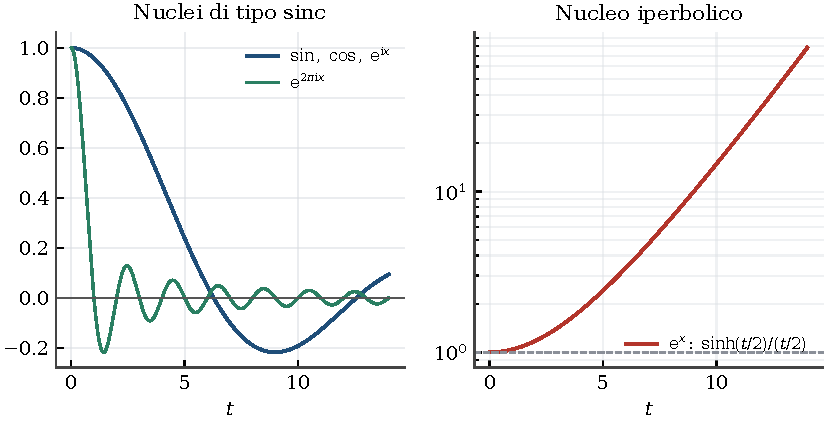
\includegraphics[width=0.86\linewidth]{../figures/trasformata_t.pdf}
  \caption{A sinistra il nucleo comune alle funzioni circolari, in due normalizzazioni. A destra il nucleo dell'esponenziale reale, in scala logaritmica: stessa formula, funzione iperbolica al posto di quella circolare, e crescita illimitata.}
  \label{fig:trasformata_t}
\end{figure}

Il rapporto non dipende da $t$: vale $2^n/(n+1)$ per ogni intervallo. Il motivo è l'omogeneità — sia il valor medio sia il valore nel punto di mezzo sono proporzionali a $t^n$, e il rapporto si semplifica.

Questa riga permette anche di riconoscere che cosa stia misurando l'operatore. Lo sviluppo di $T[f]$ per $t$ piccolo è
\[
  T[f](t)=1+\frac{t^2}{24}\,\frac{f''}{f}+O\!\left(t^4\right),
\]
che è l'errore relativo della formula di quadratura del punto medio. Per il seno $f''/f=-1$ e si ottiene $1-t^2/24$, che è lo sviluppo di $\mathrm{sinc}(t/2)$; per l'esponenziale $f''/f=+1$ e si ottiene $1+t^2/24$, cioè $\sinh(t/2)/(t/2)$; per $x^n$ valutato nel punto medio si ottiene $1+n(n-1)/6$, che coincide con $2^n/(n+1)$ per $n\le3$. L'operatore $T$, in altre parole, è l'errore della regola del punto medio scritto come funzione dell'ampiezza dell'intervallo.

\section{Le funzioni non elementari}

Le ultime sei righe applicano l'operatore a funzioni le cui primitive richiedono funzioni speciali o forme meno maneggevoli.

\begin{espr}{9}{User}{\verificata}
\begin{align*}
& \frac{\frac{1}{t}\, \int_{0}^{t} \mathrm{e}^{-x^{2}} \,\mathrm{d}x}{\mathrm{e}^{-\left(\frac{t}{2}\right)^{2}}} \\
=\;& \frac{\sqrt{\pi}\, \mathrm{e}^{\frac{t^{2}}{4}}\, \operatorname{erf}\!\left(t\right)}{2\, t}
\end{align*}
\end{espr}
La gaussiana introduce la funzione degli errori.

\begin{espr}{10}{User}{\verificata}
\begin{align*}
& \frac{\frac{1}{t}\, \int_{0}^{t} \frac{\sin\!\left(x\right)}{x} \,\mathrm{d}x}{\frac{\sin\!\left(\frac{t}{2}\right)}{\frac{t}{2}}} \\
=\;& \frac{\int_{0}^{t} \frac{\sin\!\left(x\right)}{x} \,\mathrm{d}x}{2\, \sin\!\left(\frac{t}{2}\right)}
\end{align*}
\end{espr}
L'operatore applicato al seno cardinale: il denominatore cancella il fattore $1/t$ e resta il seno integrale.

\begin{espr}{11}{User}{\verificata}
\begin{align*}
& \frac{\frac{1}{t}\, \int_{0}^{t} \arctan\!\left(x\right) \,\mathrm{d}x}{\arctan\!\left(\frac{t}{2}\right)} \\
=\;& \frac{\arctan\!\left(t\right) - \frac{\ln\!\left(t^{2} + 1\right)}{2\, t}}{\arctan\!\left(\frac{t}{2}\right)}
\end{align*}
\end{espr}
L'arcotangente: il valor medio è $\arctan t-\ln(1+t^2)/(2t)$.

\begin{espr}{12}{User}{\verificata}
\begin{align*}
& \frac{\frac{1}{t}\, \int_{0}^{t} \arcsin\!\left(x\right) \,\mathrm{d}x}{\arcsin\!\left(\frac{t}{2}\right)} \\
=\;& \frac{\arcsin\!\left(t\right) + \frac{\sqrt{1 - t^{2}} - 1}{t}}{\arcsin\!\left(\frac{t}{2}\right)}
\end{align*}
\end{espr}
L'arcoseno.

\begin{espr}{13}{User}{\verificata}
\begin{align*}
& \frac{\frac{1}{t}\, \int_{0}^{t} \arccos\!\left(x\right) \,\mathrm{d}x}{\arccos\!\left(\frac{t}{2}\right)} \\
=\;& -\frac{2\, t\, \arcsin\!\left(t\right) + 2\, \sqrt{1 - t^{2}} - \pi\, t - 2}{2\, t\, \arccos\!\left(\frac{t}{2}\right)}
\end{align*}
\end{espr}
L'arcocoseno, con la forma riordinata da Derive.

\begin{espr}{14}{User}{\verificata}
\begin{align*}
& \frac{\frac{1}{t}\, \int_{0}^{t} \tan\!\left(x\right) \,\mathrm{d}x}{\tan\!\left(\frac{t}{2}\right)} \\
=\;& \frac{-\ln\!\left(\cos\!\left(t\right)\right)\, \cot\!\left(\frac{t}{2}\right)}{t}
\end{align*}
\end{espr}
La tangente: il valor medio è $-\ln\cos t$ diviso $t$, e il risultato contiene la cotangente dell'angolo metà.


La riga $\#9$ è l'unica in cui compare una funzione speciale: il valor medio della gaussiana su $[0,t]$ è $\sqrt\pi\,\operatorname{erf}(t)/(2t)$, e dividendo per il valore nel punto medio $\mathrm{e}^{-t^2/4}$ si ottiene la forma scritta. La riga $\#10$ applica l'operatore al seno cardinale stesso, e il risultato si semplifica in modo notevole: il denominatore $\sin(t/2)/(t/2)$ cancella il fattore $1/t$ e resta il seno integrale diviso per $2\sin(t/2)$.

\section*{In sintesi}
\addcontentsline{toc}{section}{In sintesi}

Quattordici righe che dicono una cosa sola, ma la dicono bene: il rapporto fra la media di una funzione e il suo valore nel punto medio è una quantità che dipende quasi solo dalla curvatura. Per tutte le funzioni con $f''=-f$ dà il seno cardinale, per tutte quelle con $f''=+f$ il suo analogo iperbolico, per le potenze una costante. È l'ultimo quaderno della raccolta, ed è anche il più ordinato.

Il fatto ha un nome: è il caso unidimensionale del teorema della media per l'equazione di Helmholtz. Vale anche il viceversa: le funzioni per cui il rapporto fra la media su un intervallo e il valore nel suo centro dipende solo dall'ampiezza dell'intervallo sono esattamente le soluzioni di $f''=\lambda f$.


%% generato automaticamente da tools/build_tex.py --- non modificare
\chapter{Una costante travestita}
\label{cap:fxgx}
\quaderno{fx\textasciicircum{}gx.dfw}{17 Nov 2010}{10}

Novembre 2010. Dieci righe che costruiscono, per una via indiretta, una funzione che sembra dipendere da $x$ e invece non ne dipende affatto: vale $1/\mathrm{e}$ ovunque. Il percorso passa per un integrale, ed è il percorso a essere interessante, perché il risultato finale si verifica in una riga una volta che lo si ha davanti.

\section{L'integrale che genera tutto}

Le prime righe presentano una funzione e ne calcolano la primitiva. È una sostituzione classica travestita.

\begin{espr}{1}{User}{}
\[
\frac{x}{\ln\!\left(x\right)\, \ln\!\left(\ln\!\left(x\right)\right)}
\]
\end{espr}
Una funzione annotata di passaggio: il rapporto che compare nella stima della densità dei numeri primi.

\begin{espr}{2}{User}{}
\[
\frac{1}{\tan\!\left(x\right)\, \ln\!\left(\frac{1}{\sin\!\left(x\right)}\right)}
\]
\end{espr}
L'integranda vera: il reciproco del prodotto fra tangente e logaritmo del reciproco del seno.

\begin{espr}{3}{Int(\#2,x)}{}
\[
\int \frac{1}{\tan\!\left(x\right)\, \ln\!\left(\frac{1}{\sin\!\left(x\right)}\right)} \,\mathrm{d}x
\]
\end{espr}
Se ne chiede la primitiva.

\begin{espr}{4}{Simp(Int(\#2,x))}{}
\[
-\ln\!\left(\ln\!\left(\frac{1}{\sin\!\left(x\right)}\right)\right)
\]
\end{espr}
Il risultato: logaritmo di logaritmo. La sostituzione $w=\ln(1/\sin x)$ riduce tutto a $\int\mathrm{d}w/w$.


Ponendo $w=\ln\dfrac{1}{\sin x}$ si ha $\mathrm{d}w=-\cot x\,\mathrm{d}x=-\dfrac{\mathrm{d}x}{\tan x}$, e l'integrale diventa $-\displaystyle\int\frac{\mathrm{d}w}{w}=-\ln w$. Il risultato della riga $\#4$ è esattamente questo: la primitiva è il logaritmo di un logaritmo, cambiato di segno.

\section{Dall'esponenziale alla costante}

Si prende l'esponenziale della primitiva e si osserva che cosa ne viene fuori.

\begin{espr}{5}{User}{}
\[
\mathrm{e}^{-\ln\!\left(\ln\!\left(\frac{1}{\sin\!\left(x\right)}\right)\right)}
\]
\end{espr}
L'esponenziale della primitiva.

\begin{espr}{6}{Simp(\#5)}{}
\[
\frac{1}{\ln\!\left(\frac{1}{\sin\!\left(x\right)}\right)}
\]
\end{espr}
Che si semplifica nel reciproco del logaritmo.

\begin{espr}{7}{User}{}
\[
\sin^{\frac{1}{\ln\!\left(\frac{1}{\sin\!\left(x\right)}\right)}}\!\left(x\right)
\]
\end{espr}
Il seno elevato a quel reciproco. L'espressione vale $1/\mathrm{e}$ per ogni $x$ nel dominio.

\begin{espr}{8}{User}{}
\[
\cos^{\frac{1}{\ln\!\left(\frac{1}{\cos\!\left(x\right)}\right)}}\!\left(x\right)
\]
\end{espr}
La stessa costruzione con il coseno: identico risultato, perché il calcolo non usa nulla di specifico del seno.

\begin{figure}[htbp]
  \centering
  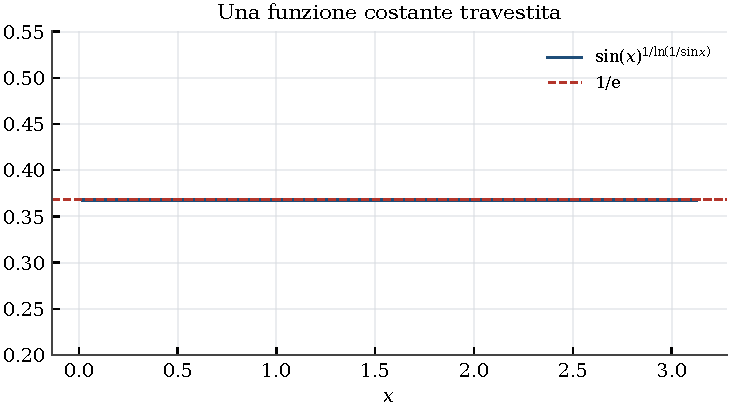
\includegraphics[width=0.86\linewidth]{../figures/fxgx.pdf}
  \caption{La funzione della riga $\#7$ tracciata su tutto il suo dominio: è la retta orizzontale $1/\mathrm{e}$. Ai due estremi il calcolo numerico si degrada, perché numeratore e denominatore dell'esponente tendono entrambi all'infinito.}
  \label{fig:fxgx}
\end{figure}

L'esponenziale della riga $\#4$ è il reciproco del logaritmo, riga $\#6$. Quel reciproco viene poi usato come esponente della funzione da cui era nato, ed è qui che la funzione collassa. Posto $u=\sin x$, l'esponente vale $\dfrac{1}{\ln(1/u)}=-\dfrac{1}{\ln u}$, e quindi
\[
  u^{\,-1/\ln u}=\exp\!\left(-\frac{\ln u}{\ln u}\right)=\mathrm{e}^{-1}.
\]
Il valore non dipende da $u$, e quindi non dipende da $x$: la riga $\#7$ è la funzione costante $1/\mathrm{e}$ scritta in modo da non sembrarlo. La riga $\#8$ ripete la costruzione con il coseno e ottiene lo stesso risultato, come deve essere: il calcolo non ha mai usato nulla del seno se non che è positivo.

\section{I due logaritmi}

Le ultime due righe isolano gli argomenti che compaiono negli esponenti.

\begin{espr}{9}{User}{}
\[
-\ln\!\left(\cos\!\left(x\right)\right)
\]
\end{espr}
Il logaritmo del reciproco del coseno, scritto con il segno esplicito.

\begin{espr}{10}{User}{}
\[
-\ln\!\left(\sin\!\left(x\right)\right)
\]
\end{espr}
E quello del seno.


Sono $-\ln\cos x$ e $-\ln\sin x$, cioè le due quantità che nel testo delle righe precedenti comparivano nella forma $\ln(1/\cos x)$ e $\ln(1/\sin x)$. Entrambe sono positive dove le funzioni trigonometriche valgono meno di uno, che è il dominio in cui la costruzione ha senso.

\section*{In sintesi}
\addcontentsline{toc}{section}{In sintesi}

Il meccanismo generale è che $u^{1/\ln u}=\mathrm{e}$ per ogni $u>0$ diverso da uno, e non c'è modo di accorgersene guardando la formula finale senza averla svolta. Il quaderno ci arriva partendo da un integrale, il che è il percorso più lungo possibile — ma è anche quello che spiega perché la costruzione fosse venuta in mente.


%% generato automaticamente da tools/build_tex.py --- non modificare
\chapter{Una regolarità che dura quattro passi}
\label{cap:factor}
\quaderno{factor.dfw}{18 Aug 2010}{36}

Agosto 2010. Il quaderno insegue un'uguaglianza fra due prodotti di fattoriali, la trova vera nei primi quattro casi, e poi la vede rompersi. Invece di abbandonarla, misura di quanto si rompe: le espressioni successive sono le fattorizzazioni complete delle differenze, numeri di trenta e più cifre scomposti nei loro fattori primi. È l'esempio migliore, in tutta la raccolta, di che cosa un sistema di calcolo simbolico permetta di fare che a mano sarebbe impensabile.

\section{Dove l'uguaglianza vale}

L'affermazione da mettere alla prova è che il prodotto dei fattoriali dei primi numeri dispari sia il fattoriale di un numero triangolare:
\[
  \prod_{n=0}^{p}(2n+1)!\;\overset{?}{=}\;\left(\frac{(p+1)(p+2)}{2}\right)!
\]
Le prime righe scrivono le differenze e le trovano nulle.

\begin{espr}{1}{User}{\verificata}
\[
1! - 1! = 0
\]
\end{espr}
Il caso $p=0$: entrambi i membri valgono $1$.

\begin{espr}{2}{User}{\verificata}
\[
1! \cdot 3! - 3! = 0
\]
\end{espr}
Il caso $p=1$: $1!\cdot3!=6=3!$.

\begin{espr}{3}{User}{\verificata}
\[
1! \cdot 3!\, 5! - 6! = 0
\]
\end{espr}
Il caso $p=2$: $720=6!$.

\begin{espr}{4}{User}{\verificata}
\[
1! \cdot 3!\, 5!\, 7! - 10! = 0
\]
\end{espr}
Il caso $p=3$: $3\,628\,800=10!$. Quattro coincidenze consecutive.


Quattro casi consecutivi, e tutti tornano: $1!=1!$, poi $1!\cdot3!=6=3!$, poi $1!\cdot3!\cdot5!=720=6!$, e infine $1!\cdot3!\cdot5!\cdot7!=3\,628\,800=10!$. I numeri $1,3,6,10$ sono i primi quattro numeri triangolari, e a questo punto una congettura è del tutto ragionevole.

\section{Dove si rompe, e di quanto}

Al quinto passo l'uguaglianza cede. Le righe seguenti non si limitano a constatarlo: fattorizzano la differenza, un caso dopo l'altro, per sei passi.

\begin{espr}{5}{User}{}
\[
1! \cdot 3!\, 5!\, 7!\, 9! - 15! = 2^{11} \cdot 3^{6}\, 5^{3}\, 7^{3}
\]
\end{espr}
Il primo caso in cui l'uguaglianza fallisce. Qui però c'è un refuso: la differenza vale $2^{11}\cdot3^{6}\cdot5^{3}\cdot7^{2}=9\,144\,576\,000$, mentre la riga scrive $7^{3}$. Il valore scritto è dunque sette volte quello vero. Tutte le fattorizzazioni successive, che sono uscite da Derive e non battute a mano, sono invece esatte.

\begin{espr}{6}{User}{\verificata}
\[
1! \cdot 3!\, 5!\, 7!\, 9!\, 11! - 21! = 2^{18} \cdot 3^{9}\, 5^{4}\, 7^{3}\, 11^{3}
\]
\end{espr}
Il caso $p=5$: la differenza contiene $11^3$.

\begin{espr}{7}{User}{\verificata}
\[
1! \cdot 3!\, 5!\, 7!\, 9!\, 11!\, 13! - 28! = 2^{25} \cdot 3^{13}\, 5^{6}\, 7^{4}\, 11^{2}\, 13\, 7103
\]
\end{espr}
Il caso $p=6$: compare il primo fattore primo estraneo ai fattoriali, $7103$.

\begin{espr}{8}{User}{\verificata}
\[
1! \cdot 3!\, 5!\, 7!\, 9!\, 11!\, 13!\, 15! - 36! = 2^{34} \cdot 3^{17}\, 5^{8}\, 7^{5}\, 11^{3}\, 13^{2}\, 4013\, 4261
\]
\end{espr}
Il caso $p=7$: due fattori primi a quattro cifre, $4013$ e $4261$.

\begin{espr}{9}{User}{\verificata}
\[
1! \cdot 3!\, 5!\, 7!\, 9!\, 11!\, 13!\, 15!\, 17! - 45! = 2^{41} \cdot 3^{21}\, 5^{10}\, 7^{6}\, 11^{5}\, 13^{3}\, 17\, 8933\, 22969787
\]
\end{espr}
Il caso $p=8$: compare $22\,969\,787$.

\begin{espr}{10}{User}{\verificata}
\begin{align*}
& 1! \cdot 3!\, 5!\, 7!\, 9!\, 11!\, 13!\, 15!\, 17!\, 19! - 55! \\
=\;& 2^{50} \cdot 3^{26}\, 5^{13}\, 7^{8}\, 11^{6}\, 13^{4}\, 17^{2}\, 19\, 3116563\, 333915299
\end{align*}
\end{espr}
Il caso $p=9$: compaiono $3\,116\,563$ e $333\,915\,299$. Nessuno di questi ha rapporto con i fattoriali di partenza.

\begin{espr}{11}{Fctr(User)}{}
\[
2^{64} \cdot 3^{31}\, 5^{15}\, 7^{10}\, 11^{6}\, 13^{7}\, 17^{3}\, 19^{2}\, 251\, 6184811\, 13366363319
\]
\end{espr}
Il caso $p=10$, dato solo nella forma fattorizzata.

\begin{espr}{12}{Fctr(User)}{}
\[
2^{74} \cdot 3^{36}\, 5^{18}\, 7^{12}\, 11^{7}\, 13^{7}\, 17^{4}\, 19^{3}\, 23\, 1543\, 3529737954001890223489333
\]
\end{espr}
Il caso $p=11$: l'ultimo fattore ha venticinque cifre.

\begin{espr}{13}{Fctr(User)}{}
\[
2^{86} \cdot 3^{44}\, 5^{21}\, 7^{14}\, 11^{8}\, 13^{7}\, 17^{5}\, 19^{4}\, 23^{2}\, 7527420903061154660844431547708509201
\]
\end{espr}
Il caso $p=12$: la parte non piccola è un unico numero di trentasette cifre.

\begin{espr}{14}{Fctr(User)}{}
\[
2^{101} \cdot 3^{50}\, 5^{25}\, 7^{17}\, 11^{9}\, 13^{8}\, 17^{6}\, 19^{5}\, 23^{3}\, 267661\, 669113\, 96487944706595864404794370019938759
\]
\end{espr}
Il caso $p=13$.

\begin{espr}{15}{Fctr(User)}{}
\[
2^{116} \cdot 3^{58}\, 5^{28}\, 7^{19}\, 11^{10}\, 13^{9}\, 17^{7}\, 19^{6}\, 23^{4}\, 29\, 967\, 106487\, 459130657\, 3283850683\, 26841959932382587431547457373253
\]
\end{espr}
Il caso $p=14$: la differenza contiene un fattore primo di trentadue cifre.


La rottura è netta ma non catastrofica. Al primo caso in cui fallisce, $p=4$, la differenza vale poco più di nove miliardi contro un valore comune di circa $1{,}3\cdot10^{12}$: uno scarto dello $0{,}7\%$. Ai passi successivi la differenza cresce molto più in fretta dei due prodotti, e già a $p=9$ nella sua fattorizzazione compaiono primi enormi — $3\,116\,563$ e $333\,915\,299$ — che non hanno nulla a che vedere con i piccoli fattori dei fattoriali.

È questo il segnale che la congettura non era vicina al vero ma solo fortunata all'inizio. Se la differenza fosse un errore sistematico piccolo, i suoi fattori resterebbero fra i primi che compongono i fattoriali; il fatto che compaiano fattori primi grandi e apparentemente casuali dice che i due numeri non hanno alcuna relazione aritmetica al di là della coincidenza iniziale.

\section{L'enunciato generale e i casi verificati}

Una riga sola scrive la differenza in forma generale, e le quattro seguenti riverificano i casi che funzionano mostrando anche le fattorizzazioni dei due membri.

\begin{espr}{16}{User}{}
\[
\prod_{n=0}^{p} \left(2\, n + 1\right)! - \left(\frac{\left(p + 1\right)\, \left(p + 2\right)}{2}\right)!
\]
\end{espr}
L'enunciato generale della differenza, che è ciò che tutte le righe precedenti hanno valutato.

\begin{figure}[htbp]
  \centering
  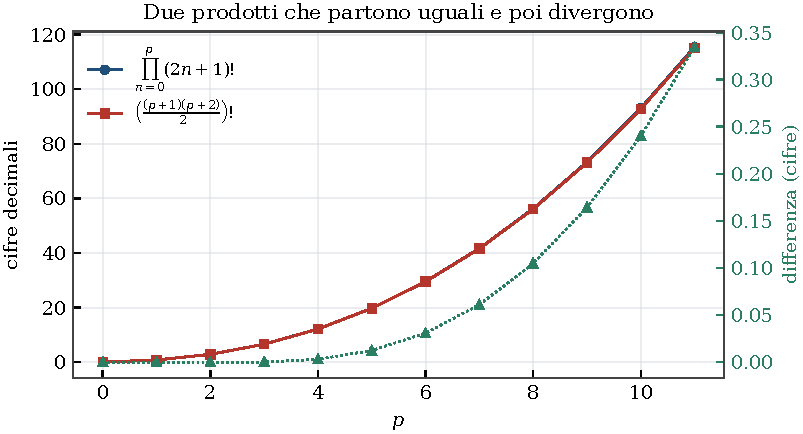
\includegraphics[width=0.86\linewidth]{../figures/factor.pdf}
  \caption{I due membri dell'uguaglianza, misurati in numero di cifre decimali. Coincidono fino a $p=3$ e poi si separano; la curva tratteggiata sull'asse destro è la loro differenza, che cresce senza limite.}
  \label{fig:factor}
\end{figure}
\begin{espr}{17}{User}{\verificata}
\[
1! = 1 = 1!
\]
\end{espr}
La verifica del caso $p=0$, con entrambi i membri.

\begin{espr}{18}{User}{\verificata}
\[
1! \cdot 3! = 2 \cdot 3 = 3!
\]
\end{espr}
Il caso $p=1$, con la fattorizzazione $2\cdot3$.

\begin{espr}{19}{User}{\verificata}
\[
1! \cdot 3!\, 5! = 2^{4} \cdot 3^{2}\, 5 = 6!
\]
\end{espr}
Il caso $p=2$: $2^4\cdot3^2\cdot5=6!$.

\begin{espr}{20}{User}{\verificata}
\[
1! \cdot 3!\, 5!\, 7! = 2^{8} \cdot 3^{4}\, 5^{2}\, 7 = 10!
\]
\end{espr}
Il caso $p=3$: $2^8\cdot3^4\cdot5^2\cdot7=10!$. È l'ultimo che funziona.


Le righe $\#17$--$\#20$ sono la stessa verifica dei primi quattro casi, ma questa volta con i due membri scritti nella loro forma fattorizzata: $2^4\cdot3^2\cdot5=720=6!$ e $2^8\cdot3^4\cdot5^2\cdot7=3\,628\,800=10!$. Serve a vedere che gli esponenti combaciano — che è il modo naturale di controllare un'uguaglianza fra prodotti di fattoriali.

\section{Le fattorizzazioni dei fattoriali triangolari}

L'ultima sezione fattorizza il secondo membro per i valori successivi, cioè i fattoriali $15!$, $21!$, $28!$, $36!$, $45!$, $55!$, $66!$, $78!$.

\begin{espr}{21}{User}{}
\[
15!
\]
\end{espr}
Il primo fattoriale triangolare per cui l'uguaglianza fallisce.

\begin{espr}{22}{Fctr(\#21)}{}
\[
2^{11} \cdot 3^{6}\, 5^{3}\, 7^{2}\, 11\, 13
\]
\end{espr}
La sua fattorizzazione. Da confrontare con la riga $\#5$: gli esponenti di $2$, $3$ e $5$ coincidono, quello di $7$ no, e in più compaiono $11$ e $13$.

\begin{espr}{23}{User}{}
\[
21!
\]
\end{espr}
Il fattoriale successivo.

\begin{espr}{24}{Fctr(\#23)}{}
\[
2^{18} \cdot 3^{9}\, 5^{4}\, 7^{3}\, 11\, 13\, 17\, 19
\]
\end{espr}
La sua fattorizzazione.

\begin{espr}{25}{User}{}
\[
28!
\]
\end{espr}
E il successivo.

\begin{espr}{26}{Fctr(\#25)}{}
\[
2^{25} \cdot 3^{13}\, 5^{6}\, 7^{4}\, 11^{2}\, 13^{2}\, 17\, 19\, 23
\]
\end{espr}
La sua fattorizzazione.

\begin{espr}{27}{User}{}
\[
\left(\frac{\left(7 + 1\right)\, \left(7 + 2\right)}{2}\right)!
\]
\end{espr}
Lo stesso numero scritto con la formula del numero triangolare.

\begin{espr}{28}{Fctr(\#27)}{}
\[
2^{34} \cdot 3^{17}\, 5^{8}\, 7^{5}\, 11^{3}\, 13^{2}\, 17^{2}\, 19\, 23\, 29\, 31
\]
\end{espr}
La sua fattorizzazione: compaiono tutti i primi fino a $31$.

\begin{espr}{29}{Sub(User)}{}
\[
\left(\frac{\left(8 + 1\right)\, \left(8 + 2\right)}{2}\right)!
\]
\end{espr}
Il passo successivo.

\begin{espr}{30}{Fctr(\#29)}{}
\[
2^{41} \cdot 3^{21}\, 5^{10}\, 7^{6}\, 11^{4}\, 13^{3}\, 17^{2}\, 19^{2}\, 23\, 29\, 31\, 37\, 41\, 43
\]
\end{espr}
La fattorizzazione arriva a $43$.

\begin{espr}{31}{Sub(\#16')}{}
\[
\left(\frac{\left(9 + 1\right)\, \left(9 + 2\right)}{2}\right)!
\]
\end{espr}
E ancora.

\begin{espr}{32}{Fctr(\#31)}{}
\[
2^{50} \cdot 3^{26}\, 5^{13}\, 7^{8}\, 11^{5}\, 13^{4}\, 17^{3}\, 19^{2}\, 23^{2}\, 29\, 31\, 37\, 41\, 43\, 47\, 53
\]
\end{espr}
Fino a $53$.

\begin{espr}{33}{Sub(\#16')}{}
\[
\left(\frac{\left(10 + 1\right)\, \left(10 + 2\right)}{2}\right)!
\]
\end{espr}
Il numero triangolare di indice dieci.

\begin{espr}{34}{Fctr(\#33)}{}
\[
2^{64} \cdot 3^{31}\, 5^{15}\, 7^{10}\, 11^{6}\, 13^{5}\, 17^{3}\, 19^{3}\, 23^{2}\, 29^{2}\, 31^{2}\, 37\, 41\, 43\, 47\, 53\, 59\, 61
\]
\end{espr}
La fattorizzazione arriva a $61$.

\begin{espr}{35}{Sub(\#16')}{}
\[
\left(\frac{\left(11 + 1\right)\, \left(11 + 2\right)}{2}\right)!
\]
\end{espr}
Quello di indice undici.

\begin{espr}{36}{Fctr(\#35)}{}
\[
2^{74} \cdot 3^{36}\, 5^{18}\, 7^{12}\, 11^{7}\, 13^{6}\, 17^{4}\, 19^{4}\, 23^{3}\, 29^{2}\, 31^{2}\, 37^{2}\, 41\, 43\, 47\, 53\, 59\, 61\, 67\, 71\, 73
\]
\end{espr}
L'ultima fattorizzazione del quaderno: tutti i primi fino a $73$, con gli esponenti dati dalla formula di Legendre.


Il confronto con le fattorizzazioni delle differenze della prima sezione è istruttivo. I fattoriali contengono tutti i primi fino al loro argomento, con esponenti che seguono la formula di Legendre; le differenze contengono invece pochi primi piccoli con esponenti alti e poi qualche primo grande isolato. Le due strutture non si assomigliano, e questo è, in sostanza, la risposta alla domanda che il quaderno si era posto.

\section*{In sintesi}
\addcontentsline{toc}{section}{In sintesi}

Un'uguaglianza vera quattro volte di seguito e poi falsa per sempre è un buon promemoria sul valore delle verifiche numeriche. Il quaderno lo raccoglie nel modo giusto: non si limita a constatare il fallimento ma lo quantifica, e la struttura dei fattori primi delle differenze dice, meglio di qualunque argomento, che la coincidenza iniziale non nascondeva nulla.

Da segnalare che l'unica riga battuta a mano di tutta la sezione — la $\#5$ — contiene un errore di trascrizione nell'esponente di $7$, mentre tutte le fattorizzazioni prodotte da Derive sono esatte. È il secondo refuso della raccolta, dopo quello di \dfw{teoria.dfw} (capitolo~\ref{cap:teoria}), e come quello sta in una riga scritta dall'autore.


%% generato automaticamente da tools/build_tex.py --- non modificare
\chapter{Un prodotto che vale $k^{-(k-1)}$}
\label{cap:fattorazionale}
\quaderno{fattorazionale.dfw}{07 Jan 2011}{14}

Gennaio 2011. Quattordici righe, undici delle quali sono valori numerici: il quaderno calcola un prodotto per $k$ da $2$ a $12$ e lascia parlare i risultati. La regolarità si vede a occhio nudo, e la dimostrazione — che il quaderno non scrive — sta in due passaggi.

\section{Il prodotto e i suoi valori}

L'oggetto studiato è il prodotto delle differenze fra i reciproci dei primi $k-1$ interi e il reciproco di $k$.

\begin{espr}{1}{User}{}
\[
\prod_{n=1}^{k - 1} \left(\frac{1}{n} - \frac{1}{k}\right)
\]
\end{espr}
Il prodotto studiato: $k-1$ fattori, tutti della forma $1/n-1/k$.

\begin{espr}{2}{Simp(Sub(\#1))}{}
\[
\frac{1}{2}
\]
\end{espr}
$k=2$: un solo fattore, $1-1/2$.

\begin{espr}{3}{Simp(Sub(\#1))}{}
\[
\frac{1}{9}
\]
\end{espr}
$k=3$: il valore è $1/9=1/3^2$.

\begin{espr}{4}{Simp(Sub(\#1))}{}
\[
\frac{1}{64}
\]
\end{espr}
$k=4$: $1/64=1/4^3$.

\begin{espr}{5}{Simp(Sub(\#1))}{}
\[
\frac{1}{625}
\]
\end{espr}
$k=5$: $1/625=1/5^4$.

\begin{espr}{6}{Simp(Sub(\#1))}{}
\[
\frac{1}{7776}
\]
\end{espr}
$k=6$: $1/7776=1/6^5$.

\begin{espr}{7}{Simp(Sub(\#1))}{}
\[
\frac{1}{117649}
\]
\end{espr}
$k=7$: $1/117649=1/7^6$.

\begin{espr}{8}{Simp(Sub(\#1))}{}
\[
\frac{1}{2097152}
\]
\end{espr}
$k=8$: $1/2\,097\,152=1/8^7$.

\begin{espr}{9}{Simp(Sub(\#1))}{}
\[
\frac{1}{43046721}
\]
\end{espr}
$k=9$: $1/43\,046\,721=1/9^8$.

\begin{espr}{10}{Simp(Sub(\#1))}{}
\[
\frac{1}{1000000000}
\]
\end{espr}
$k=10$: esattamente un miliardesimo, cioè $1/10^9$. È la riga che rende la regola indiscutibile.

\begin{espr}{11}{Simp(Sub(\#1))}{}
\[
\frac{1}{25937424601}
\]
\end{espr}
$k=11$: $1/11^{10}$.

\begin{espr}{12}{Simp(Sub(\#1))}{}
\[
\frac{1}{743008370688}
\]
\end{espr}
$k=12$: $1/12^{11}$. Undici casi consecutivi, tutti conformi.

\begin{figure}[htbp]
  \centering
  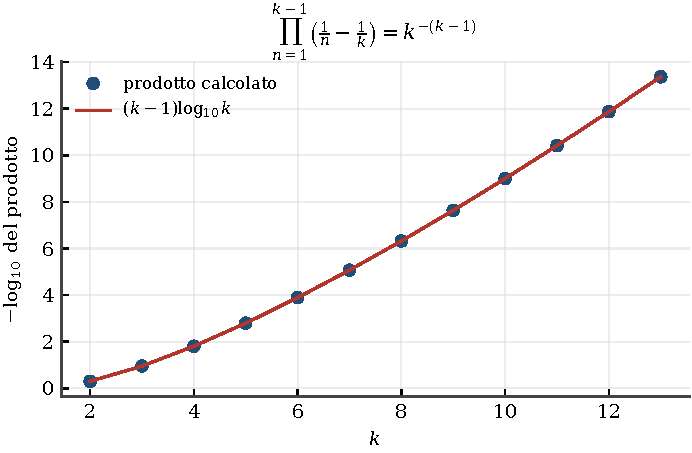
\includegraphics[width=0.86\linewidth]{../figures/fattorazionale.pdf}
  \caption{I dodici valori calcolati nel quaderno, in scala logaritmica, confrontati con la retta $(k-1)\log_{10}k$. La coincidenza è esatta, non approssimata.}
  \label{fig:fattorazionale}
\end{figure}

I valori sono $\tfrac12,\ \tfrac19,\ \tfrac1{64},\ \tfrac1{625},\ \tfrac1{7776},\ \tfrac1{117649},\dots$ e i denominatori sono $2^1,\ 3^2,\ 4^3,\ 5^4,\ 6^5,\ 7^6$: si tratta di $k^{k-1}$. La riga $\#10$ lo rende evidente anche a chi non stesse guardando: per $k=10$ il prodotto vale esattamente un miliardesimo.

La dimostrazione è breve. Scrivendo ogni fattore come $\dfrac1n-\dfrac1k=\dfrac{k-n}{nk}$, il prodotto diventa
\[
  \prod_{n=1}^{k-1}\frac{k-n}{nk}
  =\frac{\displaystyle\prod_{n=1}^{k-1}(k-n)}{k^{\,k-1}\displaystyle\prod_{n=1}^{k-1}n}
  =\frac{(k-1)!}{k^{\,k-1}\,(k-1)!}
  =\frac{1}{k^{\,k-1}},
\]
perché al numeratore compaiono gli stessi fattori del denominatore, soltanto in ordine inverso. Il nome del file — «fattoriale razionale» — allude proprio a questo: due fattoriali che si cancellano lasciando una potenza.

\section{Le due generalizzazioni}

Le ultime due righe provano ad allargare il risultato in due direzioni diverse, entrambe lasciate senza risposta.

\begin{espr}{13}{User}{}
\[
i!\, \prod_{n=1}^{k - 1} \left(\frac{1}{n} - \frac{1}{k}\right)
\]
\end{espr}
Una prima generalizzazione: il prodotto moltiplicato per un fattoriale.

\begin{espr}{14}{User}{}
\[
\prod_{i=1}^{k - n} \left(\frac{1}{i} - \frac{n}{k}\right)
\]
\end{espr}
Una seconda: il reciproco di $k$ viene sostituito da $n/k$ e il numero di fattori scende a $k-n$. Con questa modifica la cancellazione fra numeratore e denominatore non avviene più.


La riga $\#13$ moltiplica il prodotto per un fattoriale, il che equivale a chiedersi che cosa resti di $i!/k^{\,k-1}$. La riga $\#14$ è più interessante: introduce un parametro $n$ nel secondo termine e accorcia di conseguenza il numero di fattori. Ripetendo il conto si trova
\[
  \prod_{i=1}^{k-n}\left(\frac1i-\frac nk\right)
  =\frac{1}{k^{\,k-n}}\prod_{i=1}^{k-n}\frac{k-ni}{i},
\]
e il numeratore non si semplifica più con $i!$ a meno che $n=1$. La regolarità trovata è dunque un caso particolare felice, non l'inizio di una famiglia.

\section*{In sintesi}
\addcontentsline{toc}{section}{In sintesi}

Undici valori numerici e una regola che li spiega tutti. Il quaderno si ferma un attimo prima della dimostrazione, che pure è di due righe — ma i valori scelti, e in particolare quello per $k=10$, sono disposti in modo che la regola si legga da sola.


%% generato automaticamente da tools/build_tex.py --- non modificare
\chapter{Una somma sola}
\label{cap:numeri-primi}
\quaderno{numeri primi.dfw}{27 Aug 2010}{1}

Agosto 2010, lo stesso giorno di \dfw{pigreco.dfw}. Il file contiene una sola espressione, lunga 573 caratteri: la somma dei reciproci dei primi diciannove primoriali, scritta per esteso, con tutti i denominatori sviluppati come prodotti di numeri primi.

È anche il file che, durante il recupero, per un po' è sembrato vuoto. Il formato \dfw{.dfw} memorizza la lunghezza del testo in un byte, e un byte arriva a 254: le espressioni più lunghe usano una codifica estesa che il primo estrattore non riconosceva. Vedere \dfw{numeri primi.dfw} passare da zero a una espressione è stato il segnale che quella codifica esisteva.

\section{La somma}
\begin{espr}{1}{User}{}
\begin{align*}
& \frac{1}{2} + \frac{1}{2 \cdot 3} + \frac{1}{2 \cdot 3\, 5} + \frac{1}{2 \cdot 3\, 5\, 7} + \frac{1}{2 \cdot 3\, 5\, 7\, 11} + \frac{1}{2 \cdot 3\, 5\, 7\, 11\, 13} \\
&\qquad + \frac{1}{2 \cdot 3\, 5\, 7\, 11\, 13\, 17} + \frac{1}{2 \cdot 3\, 5\, 7\, 11\, 13\, 17\, 19} + \frac{1}{2 \cdot 3\, 5\, 7\, 11\, 13\, 17\, 19\, 23} + \frac{1}{2 \cdot 3\, 5\, 7\, 11\, 13\, 17\, 19\, 23\, 29} \\
&\qquad + \frac{1}{2 \cdot 3\, 5\, 7\, 11\, 13\, 17\, 19\, 23\, 29\, 31} + \frac{1}{2 \cdot 3\, 5\, 7\, 11\, 13\, 17\, 19\, 23\, 29\, 31\, 37} + \frac{1}{2 \cdot 3\, 5\, 7\, 11\, 13\, 17\, 19\, 23\, 29\, 31\, 37\, 41} \\
&\qquad + \frac{1}{2 \cdot 3\, 5\, 7\, 11\, 13\, 17\, 19\, 23\, 29\, 31\, 37\, 41\, 43} + \frac{1}{2 \cdot 3\, 5\, 7\, 11\, 13\, 17\, 19\, 23\, 29\, 31\, 37\, 41\, 43\, 47} \\
&\qquad + \frac{1}{2 \cdot 3\, 5\, 7\, 11\, 13\, 17\, 19\, 23\, 29\, 31\, 37\, 41\, 43\, 47\, 53} + \frac{1}{2 \cdot 3\, 5\, 7\, 11\, 13\, 17\, 19\, 23\, 29\, 31\, 37\, 41\, 43\, 47\, 53\, 59} \\
&\qquad + \frac{1}{2 \cdot 3\, 5\, 7\, 11\, 13\, 17\, 19\, 23\, 29\, 31\, 37\, 41\, 43\, 47\, 53\, 59\, 61} + \frac{1}{2 \cdot 3\, 5\, 7\, 11\, 13\, 17\, 19\, 23\, 29\, 31\, 37\, 41\, 43\, 47\, 53\, 59\, 61\, 67}
\end{align*}
\end{espr}
Diciannove termini, dal reciproco di $2$ al reciproco del primoriale di $67$. Ogni denominatore è il precedente moltiplicato per il primo successivo.

\begin{figure}[htbp]
  \centering
  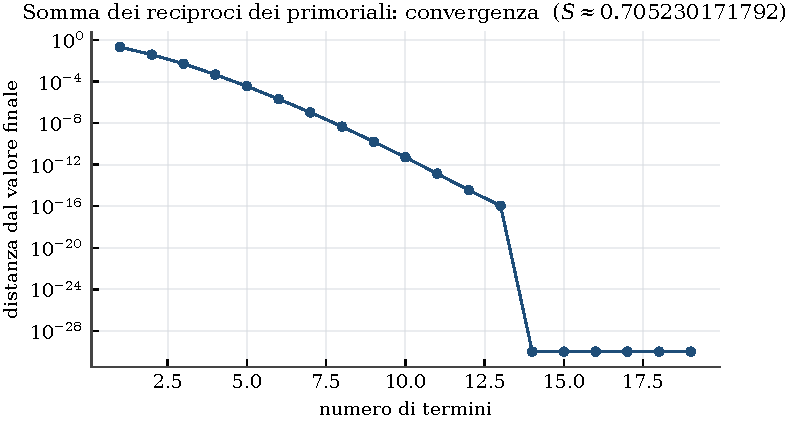
\includegraphics[width=0.86\linewidth]{../figures/primoriale.pdf}
  \caption{Distanza fra le somme parziali e il valore finale, in scala logaritmica. La convergenza è più che geometrica: ogni termine aggiunge almeno una cifra corretta, e negli ultimi passi molte di più.}
  \label{fig:primoriale}
\end{figure}

Il primoriale di $p$ è il prodotto di tutti i primi minori o uguali a $p$: $2$, poi $6$, poi $30$, $210$, $2310$, e così via. La somma dei loro reciproci converge molto rapidamente, perché ogni denominatore è almeno il doppio del precedente. I diciannove termini scritti nel quaderno — fino al primoriale di $67$, che ha venticinque cifre — danno
\[
  \sum_{n\ge1}\frac{1}{p_n\#}=0{,}70523017179180096\ldots
\]
e le cifre riportate sono già tutte quelle che i diciannove termini determinano: il ventesimo termine è dell'ordine di $10^{-27}$.

Il numero non ha una forma chiusa nota. È irrazionale — lo si dimostra con lo stesso argomento che vale per $\mathrm{e}$, perché la coda della serie dopo il termine $n$-esimo è più piccola del termine stesso — ma non se ne conosce altro. Il quaderno non aggiunge commenti, e in questo caso è comprensibile: era il posto dove annotare il valore, non dove studiarlo.

Vale la pena osservare come è scritta l'espressione. I denominatori non sono $2$, $6$, $30$, $210$: sono $2$, $2\cdot3$, $2\cdot3\cdot5$, $2\cdot3\cdot5\cdot7$. La struttura del primoriale è lasciata visibile, e la somma si legge come un elenco di primi che si allunga di uno a ogni riga.


%% generato automaticamente da tools/build_tex.py --- non modificare
\chapter{Quanto vale un gradino nel punto in cui salta}
\label{cap:u0-sign0}
\quaderno{u(0)-sign(0).dfw}{04 Jan 2011}{12}

Gennaio 2011. Il nome del file pone la domanda: quanto valgono, nell'origine, il gradino unitario $u$ e la funzione segno? La risposta convenzionale è $u(0)=1/2$ e $\mathrm{sgn}(0)=0$, scelta per simmetria. Il quaderno però arriva da un'altra strada — quella delle costruzioni di \dfw{mate.dfw} (capitolo~\ref{cap:mate}), dove il gradino nasceva come rapporto $\ln\!\left(\ldots\right)/x$ che nell'origine è una forma indeterminata — e le dodici righe che seguono confrontano quattro candidati.

Il quaderno non registra da quale funzione ciascun candidato provenga: si limita ai numeri e alle loro differenze. Le forme chiuse qui sotto sono ricostruite dai valori.

\section{I quattro candidati}

Le prime otto righe calcolano i quattro valori. Espressi in forma chiusa sono $\ln(\mathrm{e}-1)$, $\ln\sinh 1$, la media fra quest'ultimo e $1$, e il doppio del primo diminuito di uno.

\begin{espr}{1}{User}{}
\[
\ln\!\left(\mathrm{e} - 1\right)
\]
\end{espr}
Il primo candidato: $\ln(\mathrm{e}-1)$.

\begin{espr}{2}{Approx(\#1)}{}
\[
0.5413248546
\]
\end{espr}
Vale $0{,}5413248546$: poco più di un mezzo.

\begin{espr}{3}{User}{}
\[
\ln\!\left(\frac{\mathrm{e}^{2} - 1}{2\, \mathrm{e}}\right)
\]
\end{espr}
Il secondo candidato. L'argomento del logaritmo è $\sinh 1$.

\begin{espr}{4}{User}{}
\[
0.1614393615
\]
\end{espr}
Vale $0{,}1614393615$.

\begin{espr}{5}{User}{}
\[
0.5\, \left(\ln\!\left(\frac{\mathrm{e}^{2} - 1}{2\, \mathrm{e}}\right) + 1\right)
\]
\end{espr}
La media fra il secondo candidato e l'unità.

\begin{espr}{6}{Approx(\#5)}{}
\[
0.5807196807
\]
\end{espr}
Vale $0{,}5807196807$.

\begin{espr}{7}{User}{}
\[
2\, \ln\!\left(\mathrm{e} - 1\right) - 1
\]
\end{espr}
Il doppio del primo candidato, meno uno: è la trasformazione che porta dal gradino al segno.

\begin{espr}{8}{Approx(\#7)}{}
\[
0.08264970922
\]
\end{espr}
Vale $0{,}0826497092$.

\begin{figure}[htbp]
  \centering
  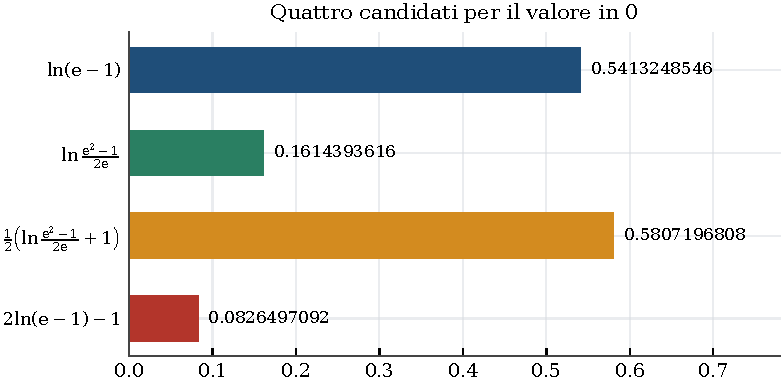
\includegraphics[width=0.86\linewidth]{../figures/u0.pdf}
  \caption{I quattro candidati a confronto. La convenzione usuale porrebbe il gradino a $0{,}5$; il candidato più vicino, $\ln(\mathrm{e}-1)$, la supera di quattro centesimi.}
  \label{fig:u0}
\end{figure}

I quattro numeri sono $0{,}5413$, $0{,}1614$, $0{,}5807$ e $0{,}0826$. Il secondo si riconosce subito: $\dfrac{\mathrm{e}^2-1}{2\mathrm{e}}=\dfrac{\mathrm{e}-\mathrm{e}^{-1}}{2}=\sinh 1$, dunque la riga $\#3$ è $\ln\sinh 1$. Il primo è $\ln(\mathrm{e}-1)$ e vale poco più di un mezzo, il che lo rende il candidato più vicino alla convenzione usuale per $u(0)$.

Le righe $\#5$ e $\#7$ sono due modi diversi di normalizzare: la prima fa la media fra $\ln\sinh1$ e $1$, la seconda raddoppia $\ln(\mathrm{e}-1)$ e sottrae $1$. Sono le stesse due operazioni che in \dfw{mate.dfw} portavano dal gradino alla funzione segno e viceversa.

\section{Le due differenze}

Le ultime quattro righe confrontano i candidati a coppie, e qui c'è una relazione esatta.

\begin{espr}{9}{User}{}
\[
0.5\, \left(\ln\!\left(\frac{\mathrm{e}^{2} - 1}{2\, \mathrm{e}}\right) + 1\right) - \ln\!\left(\mathrm{e} - 1\right)
\]
\end{espr}
La differenza fra il terzo e il primo candidato.

\begin{espr}{10}{Approx(\#9)}{}
\[
0.03939482617
\]
\end{espr}
Vale $0{,}0393948262$, cioè $\tfrac12\ln\!\left[\coth(1/2)/2\right]$.

\begin{espr}{11}{User}{}
\[
\ln\!\left(\frac{\mathrm{e}^{2} - 1}{2\, \mathrm{e}}\right) - \left(2\, \ln\!\left(\mathrm{e} - 1\right) - 1\right)
\]
\end{espr}
La differenza fra il secondo e il quarto.

\begin{espr}{12}{Approx(\#11)}{}
\[
0.07878965234
\]
\end{espr}
Vale $0{,}0787896523$, esattamente il doppio della riga $\#10$: i due scarti sono la stessa quantità misurata sulla scala del gradino e su quella del segno.


I due scarti stanno in rapporto esattamente $1$ a $2$: la riga $\#12$ vale il doppio della riga $\#10$, cifra per cifra. Non è una coincidenza numerica ma un'identità, e si vede sviluppando. Poiché $\sinh1=\dfrac{(\mathrm{e}-1)(\mathrm{e}+1)}{2\mathrm{e}}$, si ha $\ln\sinh1=\ln(\mathrm{e}-1)+\ln(\mathrm{e}+1)-\ln2-1$, e sostituendo:
\[
  \frac{\ln\sinh 1+1}{2}-\ln(\mathrm{e}-1)
  =\frac{1}{2}\ln\frac{\mathrm{e}+1}{2(\mathrm{e}-1)}
  =\frac{1}{2}\ln\frac{\coth\tfrac12}{2},
\]
mentre la riga $\#12$ dà lo stesso logaritmo senza il fattore un mezzo. Il valore comune è $\ln\coth\tfrac12-\ln2=0{,}0787896523\ldots$

Questo dice che i quattro candidati non sono indipendenti: due sono la stessa cosa a meno del riscalamento gradino-segno, e la loro distanza è la stessa quantità misurata su due scale diverse. Nessuno dei quattro vale $1/2$, e il più vicino, $\ln(\mathrm{e}-1)=0{,}5413$, se ne discosta di quattro centesimi.

\section*{In sintesi}
\addcontentsline{toc}{section}{In sintesi}

Il quaderno non conclude, e forse non poteva. La domanda «quanto vale un gradino nel punto in cui salta» non ha una risposta unica: dipende da quale famiglia di funzioni continue lo si consideri limite. La convenzione $1/2$ nasce dalla simmetria e dalla serie di Fourier; i valori raccolti qui nascono invece dalle costruzioni logaritmiche di \dfw{mate.dfw}, e sono diversi perché diverso è il limite. L'unica cosa che le dodici righe stabiliscono con certezza è la relazione esatta fra i due scarti — e quella, almeno, è un'identità.


%% generato automaticamente da tools/build_tex.py --- non modificare
\chapter{Determinanti di un sudoku}
\label{cap:sudoku}
\quaderno{Sudoku.dfw}{26 Apr 2009}{42}

Aprile 2009, il quaderno più antico insieme a \dfw{teoria.dfw}. La domanda è semplice e un po' oziosa, del genere che viene in mente guardando una griglia riempita: che cosa succede se la si tratta come una matrice? Quarantadue espressioni dopo, la risposta è che non succede granché — ma il percorso per stabilirlo è ordinato, e un fatto interessante c'è.

La griglia in esame è un sudoku valido: ogni riga, ogni colonna e ognuno dei nove blocchi contengono le cifre da $1$ a $9$ una volta sola. La verifica è stata rifatta durante il recupero e conferma.

\section{Il determinante della griglia intera}

Si comincia dalla domanda più diretta.

\begin{espr}{1}{User}{}
\[
\begin{vmatrix} 9 & 1 & 3 & 7 & 8 & 6 & 5 & 4 & 2 \\ 4 & 8 & 7 & 5 & 2 & 3 & 1 & 9 & 6 \\ 2 & 6 & 5 & 4 & 1 & 9 & 3 & 8 & 7 \\ 8 & 5 & 6 & 3 & 7 & 4 & 2 & 1 & 9 \\ 7 & 9 & 2 & 1 & 6 & 5 & 4 & 3 & 8 \\ 3 & 4 & 1 & 2 & 9 & 8 & 7 & 6 & 5 \\ 6 & 3 & 4 & 9 & 5 & 7 & 8 & 2 & 1 \\ 5 & 2 & 9 & 8 & 4 & 1 & 6 & 7 & 3 \\ 1 & 7 & 8 & 6 & 3 & 2 & 9 & 5 & 4 \end{vmatrix}
\]
\end{espr}
La griglia intera come matrice $9\times9$.

\begin{espr}{2}{Simp(\#1)}{}
\[
-2975130
\]
\end{espr}
Il suo determinante. È divisibile per $45$ — proprietà comune a tutti i sudoku — e in questo caso anche per $405$.


Il valore è $-2\,975\,130$, e ha una proprietà che vale la pena di far notare perché il quaderno non la nota: è divisibile per $45$, e la dimostrazione è di una riga. Poiché ogni riga della griglia somma a $45$, sostituendo alla prima colonna la somma di tutte le colonne si ottiene una colonna con tutti gli elementi uguali a $45$, che si raccoglie a fattore comune. Il determinante di un sudoku è dunque sempre un multiplo di $45$. In questo caso lo è anche di $405$: $-2\,975\,130=405\cdot(-7346)$, e la fattorizzazione completa è $-2\cdot3^4\cdot5\cdot3673$.

\section{I nove blocchi}

Il passo successivo è prendere i nove blocchi $3\times3$ — quelli che nel gioco devono contenere tutte le cifre — e calcolarne i determinanti uno per uno.

\begin{espr}{3}{User}{}
\[
\begin{vmatrix} 9 & 1 & 3 \\ 4 & 8 & 7 \\ 2 & 6 & 5 \end{vmatrix}
\]
\end{espr}
Il primo blocco: righe $1$--$3$, colonne $1$--$3$.

\begin{espr}{4}{User}{}
\[
0
\]
\end{espr}
Il determinante è nullo: le tre righe del blocco sono linearmente dipendenti.

\begin{espr}{5}{User}{}
\[
\begin{vmatrix} 7 & 8 & 6 \\ 5 & 2 & 3 \\ 4 & 1 & 9 \end{vmatrix}
\]
\end{espr}
Il secondo blocco.

\begin{espr}{6}{Simp(\#5)}{}
\[
-177
\]
\end{espr}
$-177$.

\begin{espr}{7}{User}{}
\[
\begin{vmatrix} 5 & 4 & 2 \\ 1 & 9 & 6 \\ 3 & 8 & 7 \end{vmatrix}
\]
\end{espr}
Il terzo blocco.

\begin{espr}{8}{Simp(\#7)}{}
\[
81
\]
\end{espr}
$81$.

\begin{espr}{9}{User}{}
\[
\begin{vmatrix} 8 & 5 & 6 \\ 7 & 9 & 2 \\ 3 & 4 & 1 \end{vmatrix}
\]
\end{espr}
Il quarto blocco.

\begin{espr}{10}{Simp(\#9)}{}
\[
9
\]
\end{espr}
$9$.

\begin{espr}{11}{User}{}
\[
\begin{vmatrix} 3 & 7 & 4 \\ 1 & 6 & 5 \\ 2 & 9 & 8 \end{vmatrix}
\]
\end{espr}
Il quinto blocco, quello centrale.

\begin{espr}{12}{User}{}
\[
11
\]
\end{espr}
$11$.

\begin{espr}{13}{User}{}
\[
\begin{vmatrix} 2 & 1 & 9 \\ 4 & 3 & 8 \\ 7 & 6 & 5 \end{vmatrix}
\]
\end{espr}
Il sesto blocco.

\begin{espr}{14}{Simp(\#13)}{}
\[
-3
\]
\end{espr}
$-3$.

\begin{espr}{15}{User}{}
\[
\begin{vmatrix} 6 & 3 & 4 \\ 5 & 2 & 9 \\ 1 & 7 & 8 \end{vmatrix}
\]
\end{espr}
Il settimo blocco.

\begin{espr}{16}{Simp(\#15)}{}
\[
-243
\]
\end{espr}
$-243$.

\begin{espr}{17}{User}{}
\[
\begin{vmatrix} 9 & 5 & 7 \\ 8 & 4 & 1 \\ 6 & 3 & 2 \end{vmatrix}
\]
\end{espr}
L'ottavo blocco.

\begin{espr}{18}{Simp(\#17)}{}
\[
-5
\]
\end{espr}
$-5$.

\begin{espr}{19}{User}{}
\[
\begin{vmatrix} 8 & 2 & 1 \\ 6 & 7 & 3 \\ 9 & 5 & 4 \end{vmatrix}
\]
\end{espr}
Il nono blocco.

\begin{espr}{20}{Simp(User)}{}
\[
77
\]
\end{espr}
$77$.

\begin{espr}{21}{User}{}
\[
0 + -177 + 81 + 9 + 11 + -3 + -243 + -5 + 77
\]
\end{espr}
La somma dei nove valori, scritta per esteso.

\begin{espr}{22}{Simp(\#21)}{}
\[
-250
\]
\end{espr}
Vale $-250$.

\begin{figure}[htbp]
  \centering
  % La griglia studiata in Sudoku.dfw e i determinanti dei nove blocchi.
\begin{tikzpicture}[scale=0.56, every node/.style={font=\small}]

  % ---- la griglia ---------------------------------------------------
  \begin{scope}
    \def\griglia{
      {9,1,3,7,8,6,5,4,2},
      {4,8,7,5,2,3,1,9,6},
      {2,6,5,4,1,9,3,8,7},
      {8,5,6,3,7,4,2,1,9},
      {7,9,2,1,6,5,4,3,8},
      {3,4,1,2,9,8,7,6,5},
      {6,3,4,9,5,7,8,2,1},
      {5,2,9,8,4,1,6,7,3},
      {1,7,8,6,3,2,9,5,4}}

    \foreach \bi in {0,1,2}{
      \foreach \bj in {0,1,2}{
        \pgfmathtruncatemacro{\tinta}{mod(\bi+\bj,2)}
        \ifnum\tinta=0
          \fill[grigiocarta] (3*\bj,-3*\bi) rectangle ++(3,-3);
        \fi
      }}

    \foreach \r [count=\i from 0] in \griglia {
      \foreach \v [count=\j from 0] in \r {
        \node[inchiostro] at (\j+0.5,-\i-0.5) {\v};
      }}

    \foreach \k in {0,...,9}{
      \draw[grigiotratto,line width=0.5pt] (\k,0) -- (\k,-9);
      \draw[grigiotratto,line width=0.5pt] (0,-\k) -- (9,-\k);
    }
    \foreach \k in {0,3,6,9}{
      \draw[blunotte,line width=1.1pt] (\k,0) -- (\k,-9);
      \draw[blunotte,line width=1.1pt] (0,-\k) -- (9,-\k);
    }
    \node[grigiotesto,font=\footnotesize\sffamily,anchor=north] at (4.5,-9.3)
      {la griglia};
  \end{scope}

  % ---- i determinanti dei blocchi -----------------------------------
  \begin{scope}[xshift=11.2cm]
    % celle larghe 2 e alte 2.5, per allinearsi ai blocchi della griglia
    \foreach \d [count=\n from 0] in {0,-177,81,9,11,-3,-243,-5,77}{
      \pgfmathtruncatemacro{\bi}{div(\n,3)}
      \pgfmathtruncatemacro{\bj}{mod(\n,3)}
      \node[rossoterra] at (2*\bj+1,{-0.75-2.5*\bi}) {$\d$};
    }
    \foreach \k in {2,4}{
      \draw[grigiotratto,line width=0.5pt] (\k,0.5) -- (\k,-7);
    }
    \foreach \k in {1,2}{
      \draw[grigiotratto,line width=0.5pt] (0,{0.5-2.5*\k}) -- (6,{0.5-2.5*\k});
    }
    \draw[blunotte,line width=1.1pt] (0,0.5) rectangle (6,-7);
    \node[grigiotesto,font=\footnotesize\sffamily,anchor=north,align=center]
      at (3,-7.4)
      {determinante di ciascun blocco\\[2pt] somma: $-250$};
  \end{scope}

  % ---- didascalia complessiva ---------------------------------------
  \node[grigiotesto,font=\footnotesize\sffamily,anchor=north] at (8.6,-10.6)
    {determinante della griglia intera: $-2\,975\,130=-2\cdot3^4\cdot5\cdot3673$};
\end{tikzpicture}

  \caption{La griglia del quaderno. Accanto, in rosso, il determinante di ciascun blocco $3\times3$: quello in alto a sinistra è nullo, cioè il blocco è singolare.}
  \label{fig:sudoku_griglia}
\end{figure}

I nove valori sono $0$, $-177$, $81$, $9$, $11$, $-3$, $-243$, $-5$, $77$, e la loro somma è $-250$. Tutti i valori sono stati ricalcolati durante il recupero e coincidono, compreso lo zero del primo blocco — che è l'unico caso interessante del gruppo, perché segnala che le tre righe di quel blocco sono linearmente dipendenti.

La somma $-250$ non ha alcun rapporto con il determinante della griglia intera, e non c'è motivo perché ne abbia: il determinante di una matrice a blocchi non è una funzione dei determinanti dei blocchi, a meno che la matrice non sia triangolare a blocchi. Il quaderno lo verifica sperimentalmente, che è un modo legittimo di rispondersi.

\section{Le nove righe rimodellate}

Seconda idea, diversa dalla prima: invece dei blocchi, si prende ogni riga della griglia e la si ripiega in una matrice $3\times3$. Nove righe, nove matrici, nove determinanti.

\begin{espr}{23}{User}{}
\[
\begin{vmatrix} 9 & 1 & 3 \\ 7 & 8 & 6 \\ 5 & 4 & 2 \end{vmatrix}
\]
\end{espr}
La prima riga della griglia ripiegata in una matrice $3\times3$.

\begin{espr}{24}{Simp(\#23)}{}
\[
-92
\]
\end{espr}
$-92$.

\begin{espr}{25}{User}{}
\[
\begin{vmatrix} 4 & 8 & 7 \\ 5 & 2 & 3 \\ 1 & 9 & 6 \end{vmatrix}
\]
\end{espr}
La seconda riga.

\begin{espr}{26}{Simp(\#25)}{}
\[
25
\]
\end{espr}
$25$.

\begin{espr}{27}{User}{}
\[
\begin{vmatrix} 2 & 6 & 5 \\ 4 & 1 & 9 \\ 3 & 8 & 7 \end{vmatrix}
\]
\end{espr}
La terza riga. Il valore, $9$, è quello usato nella somma della riga $\#41$.

\begin{espr}{28}{Simp(\#27)}{}
\[
9
\]
\end{espr}
\begin{espr}{29}{User}{}
\[
\begin{vmatrix} 8 & 5 & 6 \\ 3 & 7 & 4 \\ 2 & 1 & 9 \end{vmatrix}
\]
\end{espr}
La quarta riga.

\begin{espr}{30}{Simp(\#29)}{}
\[
311
\]
\end{espr}
$311$.

\begin{espr}{31}{User}{}
\[
\begin{vmatrix} 7 & 9 & 2 \\ 1 & 6 & 5 \\ 4 & 3 & 8 \end{vmatrix}
\]
\end{espr}
La quinta riga.

\begin{espr}{32}{Simp(\#31)}{}
\[
297
\]
\end{espr}
$297$.

\begin{espr}{33}{User}{}
\[
\begin{vmatrix} 3 & 4 & 1 \\ 2 & 9 & 8 \\ 7 & 6 & 5 \end{vmatrix}
\]
\end{espr}
La sesta riga.

\begin{espr}{34}{Simp(\#33)}{}
\[
124
\]
\end{espr}
$124$.

\begin{espr}{35}{User}{}
\[
\begin{vmatrix} 6 & 3 & 4 \\ 9 & 5 & 7 \\ 8 & 2 & 1 \end{vmatrix}
\]
\end{espr}
La settima riga.

\begin{espr}{36}{Simp(\#35)}{}
\[
-1
\]
\end{espr}
$-1$.

\begin{espr}{37}{User}{}
\[
\begin{vmatrix} 5 & 2 & 9 \\ 8 & 4 & 1 \\ 6 & 7 & 3 \end{vmatrix}
\]
\end{espr}
L'ottava riga.

\begin{espr}{38}{Simp(\#37)}{}
\[
277
\]
\end{espr}
$277$.

\begin{espr}{39}{User}{}
\[
\begin{vmatrix} 1 & 7 & 8 \\ 6 & 3 & 2 \\ 9 & 5 & 4 \end{vmatrix}
\]
\end{espr}
La nona riga.

\begin{espr}{40}{Simp(\#39)}{}
\[
-16
\]
\end{espr}
$-16$.

\begin{espr}{41}{User}{}
\[
-92 + 25 + 9 + 311 + 297 + 124 - 1 + 277 - 16
\]
\end{espr}
La somma dei nove valori.

\begin{espr}{42}{Simp(\#41)}{}
\[
934
\]
\end{espr}
Vale $934$.


I nove valori sono $-92$, $25$, $9$, $311$, $297$, $124$, $-1$, $277$, $-16$, e sommano a $934$. Anche questi coincidono tutti con il ricalcolo.

Né $-250$ né $934$ hanno un rapporto riconoscibile con $-2\,975\,130$, e nessuno dei due è multiplo di $45$: la proprietà di divisibilità vale per la griglia intera perché dipende dalle somme di righe e colonne, che nei sottoblocchi non sono $45$.

\section*{In sintesi}
\addcontentsline{toc}{section}{In sintesi}

Il quaderno pone una domanda e ottiene una risposta negativa: i determinanti dei sottoblocchi di un sudoku non dicono nulla sul determinante della griglia, e le loro somme non sono invarianti significativi. È una risposta utile quanto una affermativa, e per ottenerla servivano diciannove determinanti calcolati a mano — che nel 2009, con Derive aperto sullo schermo, erano diciannove righe.


%% generato automaticamente da tools/build_tex.py --- non modificare
\chapter{Un filtro elimina-banda}
\label{cap:notch}
\quaderno{notch.dfw}{21 Jan 2010}{20}

Gennaio 2010. È l'unico quaderno della raccolta che non fa matematica per sé stessa: qui si progetta un circuito. Il nome del file lo dice — un \emph{notch} è un filtro elimina-banda, quello che sopprime una frequenza precisa lasciando passare tutto il resto, e che si usa per esempio per togliere il ronzio di rete da un segnale.

Una nota di lettura. Le grandezze con pedice — la pulsazione di antirisonanza $\omega_n$, quella di taglio $\omega_0$ — nel file sono scritte \der{w*n} e \der{w*0}, cioè come prodotti. Derive non aveva i pedici nella riga di comando, e chi scriveva ha usato la moltiplicazione come surrogato tipografico. Le formule vanno lette tenendone conto.

\section{Il blocco risonante}

Si parte dall'impedenza del parallelo fra induttore e condensatore, scritta nel dominio della variabile complessa $s$.

\begin{espr}{1}{User}{}
\[
\frac{s\, l\, \left(\frac{1}{s\, c}\right)}{s\, l + \frac{1}{s\, c}}
\]
\end{espr}
L'impedenza del parallelo fra induttore e condensatore: diverge all'antirisonanza.

\begin{espr}{2}{Sub(User)}{}
\[
\frac{s\, f\, \left(\frac{1}{s\, g}\right)\, r}{s\, f\, \left(\frac{1}{s\, g} + r\right) + \frac{1}{s\, g}\, r}
\]
\end{espr}
La stessa struttura con i componenti del ramo di uscita.

\begin{espr}{3}{User}{}
\[
\frac{\frac{s\, f\, \left(\frac{1}{s\, g}\right)\, r}{s\, f\, \left(\frac{1}{s\, g} + r\right) + \frac{1}{s\, g}\, r}}{\frac{s\, l\, \left(\frac{1}{s\, c}\right)}{s\, l + \frac{1}{s\, c}} + \frac{s\, f\, \left(\frac{1}{s\, g}\right)\, r}{s\, f\, \left(\frac{1}{s\, g} + r\right) + \frac{1}{s\, g}\, r}}
\]
\end{espr}
Il partitore completo: impedenza di uscita diviso impedenza totale.

\begin{espr}{4}{Fctr(User)}{}
\[
\frac{f\, r\, \left(c\, l\, s^{2} + 1\right)}{f\, l\, r\, s^{2}\, \left(c + g\right) + f\, l\, s + r\, \left(f + l\right)}
\]
\end{espr}
Fattorizzato. Il numeratore contiene $1+s^2LC$: è lo zero che produce il notch.

\begin{figure}[htbp]
  \centering
  % Lo schema del partitore studiato in notch.dfw.
% I componenti sono rettangoli con etichetta diritta: la rotazione dei nodi
% ruoterebbe anche il testo.
\begin{tikzpicture}[
    filo/.style={draw=inchiostro,line width=0.8pt},
    lab/.style={font=\footnotesize\sffamily,color=grigiotesto},
    nome/.style={font=\small}
  ]
  % --- componenti orizzontali (larghezza 1.4, altezza 0.5) -----------
  \newcommand{\comporizz}[3]{%
    \fill[white] (#1-0.7,#2-0.28) rectangle (#1+0.7,#2+0.28);
    \draw[filo] (#1-0.7,#2-0.28) rectangle (#1+0.7,#2+0.28);
    \node[nome] at (#1,#2) {#3};}
  % --- componenti verticali (larghezza 0.56, altezza 1.2) ------------
  \newcommand{\compvert}[3]{%
    \fill[white] (#1-0.28,#2-0.6) rectangle (#1+0.28,#2+0.6);
    \draw[filo] (#1-0.28,#2-0.6) rectangle (#1+0.28,#2+0.6);
    \node[nome] at (#1,#2) {#3};}

  % --- rete ----------------------------------------------------------
  \draw[filo] (0,3) -- (1.2,3);                    % ingresso
  \draw[filo] (1.2,3) -- (4.6,3);                  % ramo con L
  \draw[filo] (1.2,3) -- (1.2,4.3) -- (4.6,4.3) -- (4.6,3);   % ramo con C
  \comporizz{2.9}{3}{$L$}
  \comporizz{2.9}{4.3}{$C$}

  \draw[filo] (4.6,3) -- (8.2,3);                  % verso l'uscita
  \draw[filo] (5.6,3) -- (5.6,0);                  % ramo di R
  \compvert{5.6}{1.5}{$R$}
  \draw[filo] (7.2,3) -- (7.2,0);                  % ramo F--G
  \compvert{7.2}{2.0}{$F$}
  \compvert{7.2}{0.7}{$G$}

  \draw[filo] (0,3) -- (0,0) -- (8.2,0);           % massa
  \draw[filo] (8.2,3) -- (8.2,3);

  % --- morsetti e etichette ------------------------------------------
  \foreach \p in {(0,3),(0,0),(8.2,3),(8.2,0)}{\fill[inchiostro] \p circle (1.5pt);}
  \node[lab,anchor=east] at (-0.15,3) {ingresso};
  \node[lab,anchor=east] at (-0.15,0) {massa};
  \node[lab,anchor=west] at (8.35,3) {uscita};

  \draw[grigiotratto,line width=0.6pt] (1.2,4.75) -- (1.2,5.05)
        -- (4.6,5.05) -- (4.6,4.75);
  \node[lab,anchor=south] at (2.9,5.1)
    {trappola $LC$: impedenza infinita a $\omega_n=1/\sqrt{LC}$};

  \draw[grigiotratto,line width=0.6pt] (5.0,-0.35) -- (5.0,-0.6)
        -- (7.8,-0.6) -- (7.8,-0.35);
  \node[lab,anchor=north] at (6.4,-0.7)
    {carico: $R$ in parallelo alla serie $F$--$G$};
\end{tikzpicture}

  \caption{Lo schema studiato nel quaderno. La serie risonante $LC$ in alto presenta impedenza infinita alla pulsazione $\omega_n$ e produce lo zero della trasferenza; il ramo di uscita determina i poli.}
  \label{fig:notch_circuito}
\end{figure}

L'impedenza del parallelo $LC$ è $\dfrac{sL\cdot\frac{1}{sC}}{sL+\frac{1}{sC}}=\dfrac{sL}{1+s^2LC}$: diverge quando $1+s^2LC=0$, cioè per $s=\pm\mathrm{i}/\sqrt{LC}$. Alla pulsazione $\omega_n=1/\sqrt{LC}$ il blocco si comporta come un circuito aperto e non lascia passare nulla: è questo che produce il notch.

La riga $\#4$ è la funzione di trasferimento completa del partitore, fattorizzata da Derive. Il numeratore contiene $\left(1+s^2LC\right)$, che si annulla esattamente alla pulsazione di antirisonanza: lo zero della trasferenza è il notch.

\section{Le varianti del carico}

Le righe seguenti calcolano la stessa trasferenza per diverse configurazioni del ramo di uscita: il solo resistore, il resistore in serie a un condensatore, il resistore in parallelo a un induttore.

\begin{espr}{5}{User}{}
\[
\frac{r}{r + \frac{s\, l\, \left(\frac{1}{s\, c}\right)}{s\, l + \frac{1}{s\, c}}}
\]
\end{espr}
La variante con il solo resistore di carico.

\begin{espr}{6}{Simp(\#5)}{}
\[
\frac{r\, \left(c\, l\, s^{2} + 1\right)}{c\, l\, r\, s^{2} + l\, s + r}
\]
\end{espr}
Semplificata. Denominatore di secondo grado, come atteso.

\begin{espr}{7}{User}{}
\[
\frac{\frac{\frac{r}{s\, g}}{\frac{1}{s\, g} + r}}{\frac{s\, l\, \left(\frac{1}{s\, c}\right)}{s\, l + \frac{1}{s\, c}} + \frac{\frac{r}{s\, g}}{\frac{1}{s\, g} + r}}
\]
\end{espr}
La variante con il resistore in parallelo al condensatore aggiuntivo.

\begin{espr}{8}{Fctr(User)}{}
\[
\frac{r\, \left(c\, l\, s^{2} + 1\right)}{l\, r\, s^{2}\, \left(c + g\right) + l\, s + r}
\]
\end{espr}
Fattorizzata: al denominatore compare la somma $C+G$.

\begin{espr}{9}{User}{}
\[
\frac{\frac{s\, f\, r}{s\, f + r}}{\frac{s\, l\, \left(\frac{1}{s\, c}\right)}{s\, l + \frac{1}{s\, c}} + \frac{s\, f\, r}{s\, f + r}}
\]
\end{espr}
La variante con l'induttore aggiuntivo in parallelo al resistore.

\begin{espr}{10}{Fctr(User)}{}
\[
\frac{f\, r\, \left(c\, l\, s^{2} + 1\right)}{c\, f\, l\, r\, s^{2} + f\, l\, s + r\, \left(f + l\right)}
\]
\end{espr}
Fattorizzata: qui compare la somma $F+L$.


Tutte le varianti condividono il fattore $\left(1+s^2LC\right)$ al numeratore — il notch non dipende dal carico — e differiscono soltanto nel denominatore, cioè nella posizione dei poli. È la separazione corretta del problema: gli zeri li mette la trappola $LC$, i poli il resto della rete.

\section{I casi limite}

Quattro righe che verificano il comportamento agli estremi, mandando all'infinito o a zero i due componenti aggiuntivi.

\begin{espr}{11}{Lim(User,f)}{}
\[
\lim_{f \to \infty} \frac{f\, r\, \left(c\, l\, s^{2} + 1\right)}{f\, l\, r\, s^{2}\, \left(c + g\right) + f\, l\, s + r\, \left(f + l\right)}
\]
\end{espr}
Il limite per induttanza aggiuntiva infinita, cioè circuito aperto.

\begin{espr}{12}{Fctr(User)}{}
\[
\frac{r\, \left(c\, l\, s^{2} + 1\right)}{l\, r\, s^{2}\, \left(c + g\right) + l\, s + r}
\]
\end{espr}
Il risultato coincide con la variante $\#8$: il controllo torna.

\begin{espr}{13}{Lim(User,g)}{}
\[
\lim_{g \to 0} \frac{f\, r\, \left(c\, l\, s^{2} + 1\right)}{f\, l\, r\, s^{2}\, \left(c + g\right) + f\, l\, s + r\, \left(f + l\right)}
\]
\end{espr}
Il limite per capacità aggiuntiva nulla.

\begin{espr}{14}{Fctr(User)}{}
\[
\frac{f\, r\, \left(c\, l\, s^{2} + 1\right)}{c\, f\, l\, r\, s^{2} + f\, l\, s + r\, \left(f + l\right)}
\]
\end{espr}
Il risultato coincide con la variante $\#10$.


Sono i controlli che si fanno sempre su una formula di rete: se un componente sparisce, la trasferenza deve ridursi a quella della rete più semplice. Entrambi i limiti tornano, e il fattore $\left(1+s^2LC\right)$ sopravvive in tutti e quattro i casi.

\section{La forma canonica}

Le ultime righe riscrivono la trasferenza nella forma standard del secondo ordine, quella in cui i parametri hanno un significato immediato.

\begin{espr}{15}{User}{}
\[
\frac{\frac{c}{g + c}\, \left(s^{2} + \frac{1}{l\, c}\right)}{s^{2} + \frac{s}{r\, \left(c + g\right)} + r\, \left(\frac{l + f}{l\, f}\right)\, \left(\frac{1}{c + g}\right)}
\]
\end{espr}
La forma canonica del secondo ordine, con il fattore di guadagno esplicito. Il termine costante del denominatore contiene però un fattore $R$ di troppo, che lo rende dimensionalmente incoerente: si veda la riga successiva.

\begin{espr}{16}{User}{}
\[
\frac{\frac{c}{g + c}\, \left(s^{2} + \frac{1}{l\, c}\right)}{s^{2} + \frac{s}{r\, \left(c + g\right)} + \frac{l + f}{l\, f}\, \left(\frac{1}{c + g}\right)}
\]
\end{espr}
La stessa scrittura senza il fattore $R$ nel termine costante: è questa la forma corretta, che coincide con la funzione di trasferimento delle righe $\#4$ e $\#10$. L'autore corregge qui la svista della riga $\#15$.

\begin{espr}{17}{User}{}
\[
a = \frac{c}{g + c}
\]
\end{espr}
Il guadagno: partitore fra le due capacità.

\begin{espr}{18}{User}{}
\[
w\, n = \sqrt{\frac{1}{l\, c}}
\]
\end{espr}
La pulsazione del notch, determinata dalla sola trappola $LC$.

\begin{espr}{19}{User}{}
\[
w\, 0 = \sqrt{\frac{1}{\frac{l\, f}{l + f}\, \left(c + g\right)}}
\]
\end{espr}
La pulsazione dei poli: coinvolge il parallelo delle induttanze e la somma delle capacità.

\begin{espr}{20}{User}{}
\[
q = r\, \left(c + g\right)\, w\, 0
\]
\end{espr}
Il fattore di merito, che fissa la larghezza della tacca.

\begin{figure}[htbp]
  \centering
  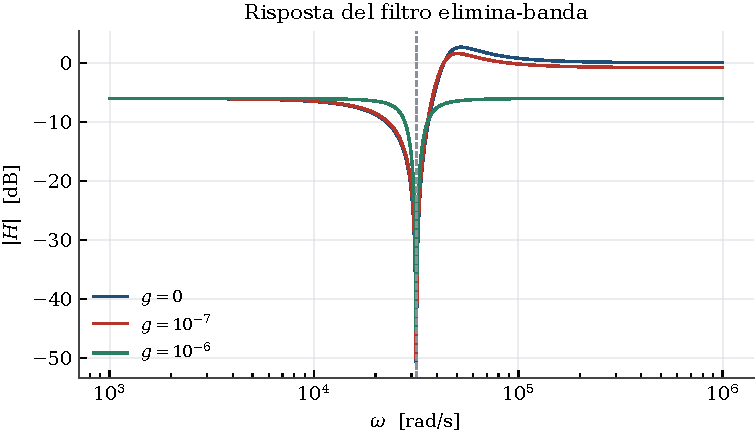
\includegraphics[width=0.86\linewidth]{../figures/notch_bode.pdf}
  \caption{Modulo della trasferenza della riga $\#4$ per tre valori della capacità aggiuntiva $G$. La tacca è alla pulsazione $\omega_n=1/\sqrt{LC}$ e non si sposta al variare del carico, mentre la profondità e la larghezza dipendono dai poli.}
  \label{fig:notch_bode}
\end{figure}

La forma è
\[
  H(s)=a\;\frac{s^2+\omega_n^2}{s^2+\dfrac{\omega_0}{Q}\,s+\omega_0^2},
\]
e le ultime quattro righe ne identificano i parametri:
\begin{itemize}[leftmargin=1.4em,itemsep=1pt]
  \item il guadagno in alta frequenza $a=\dfrac{C}{C+G}$, cioè il partitore capacitivo puro;
  \item la pulsazione del notch $\omega_n=\dfrac{1}{\sqrt{LC}}$, dove la trasferenza si annulla;
  \item la pulsazione dei poli $\omega_0=\dfrac{1}{\sqrt{\frac{LF}{L+F}\,(C+G)}}$, che coinvolge il parallelo delle due induttanze e la somma delle due capacità;
  \item il fattore di merito $Q=R(C+G)\,\omega_0$, che governa quanto stretta sia la banda soppressa.
\end{itemize}
È la forma in cui un filtro si progetta davvero: si sceglie $\omega_n$ in base alla frequenza da eliminare, e poi $Q$ in base a quanto stretta debba essere la tacca.

\section*{In sintesi}
\addcontentsline{toc}{section}{In sintesi}

Venti righe che portano un circuito dalla topologia alla forma canonica, con i controlli ai casi limite fatti per bene. È il quaderno meno speculativo della raccolta e l'unico che risponde a una domanda pratica; il fatto che stia nella stessa cartella insieme alle delta complesse e ai fattoriali semi-interi dice qualcosa su come venissero usati questi file.




% ===========================================================================
\appendix
\part{Appendici}
% ---------------------------------------------------------------------------
\chapter{Prospetto dei quaderni}
\label{app:prospetto}

La tabella elenca i ventitr\'e file nell'ordine in cui compaiono nel volume.
La colonna \emph{Espr.} d\`a il numero di espressioni recuperate, la colonna
\emph{Verif.} quante di esse hanno superato il controllo numerico descritto
nel capitolo~\ref{cap:verifica}. Si ricordi che un valore basso in
quest'ultima colonna dice soprattutto che il quaderno contiene equazioni da
risolvere o calcoli di lavoro, non identit\`a da controllare.

\begin{longtable}{@{}l l r r r@{}}
\toprule
\textbf{File} & \textbf{Data di salvataggio} & \textbf{Espr.} & \textbf{Verif.} & \textbf{Pag.} \\
\midrule
\endfirsthead
\toprule
\textbf{File} & \textbf{Data di salvataggio} & \textbf{Espr.} & \textbf{Verif.} & \textbf{Pag.} \\
\midrule
\endhead
\texttt{teoria.dfw} & 06 May 2009 & 27 & 0 & \pageref{cap:teoria} \\
\texttt{teoria2.dfw} & 02 Nov 2009 & 31 & 0 & \pageref{cap:teoria2} \\
\texttt{limit.dfw} & 19 Dec 2009 & 1 & 0 & \pageref{cap:limit} \\
\texttt{e.dfw} & 27 Aug 2010 & 93 & 15 & \pageref{cap:e} \\
\texttt{pigreco.dfw} & 27 Aug 2010 & 26 & 2 & \pageref{cap:pigreco} \\
\texttt{sin-cos.dfw} & 04 Jan 2010 & 20 & 9 & \pageref{cap:sin-cos} \\
\texttt{j.dfw} & 07 Jul 2009 & 7 & 3 & \pageref{cap:j} \\
\texttt{atan.dfw} & 28 Jan 2010 & 14 & 8 & \pageref{cap:atan} \\
\texttt{equazioni.dfw} & 27 Jan 2010 & 44 & 0 & \pageref{cap:equazioni} \\
\texttt{mate.dfw} & 18 Aug 2010 & 133 & 35 & \pageref{cap:mate} \\
\texttt{mate copia.dfw} & 09 Feb 2010 & 127 & 34 & \pageref{cap:mate-copia} \\
\texttt{cosinc.dfw} & 14 Nov 2010 & 29 & 3 & \pageref{cap:cosinc} \\
\texttt{cost\textasciicircum{}2.dfw} & 24 Jun 2010 & 22 & 0 & \pageref{cap:cost2} \\
\texttt{gauss.dfw} & 15 Sep 2010 & 14 & 3 & \pageref{cap:gauss} \\
\texttt{delta.dfw} & 13 Jul 2010 & 55 & 7 & \pageref{cap:delta} \\
\texttt{Trasformata T.dfw} & 17 Jan 2011 & 14 & 13 & \pageref{cap:trasformata-t} \\
\texttt{fx\textasciicircum{}gx.dfw} & 17 Nov 2010 & 10 & 0 & \pageref{cap:fxgx} \\
\texttt{factor.dfw} & 18 Aug 2010 & 36 & 13 & \pageref{cap:factor} \\
\texttt{fattorazionale.dfw} & 07 Jan 2011 & 14 & 0 & \pageref{cap:fattorazionale} \\
\texttt{numeri primi.dfw} & 27 Aug 2010 & 1 & 0 & \pageref{cap:numeri-primi} \\
\texttt{u(0)-sign(0).dfw} & 04 Jan 2011 & 12 & 0 & \pageref{cap:u0-sign0} \\
\texttt{Sudoku.dfw} & 26 Apr 2009 & 42 & 0 & \pageref{cap:sudoku} \\
\texttt{notch.dfw} & 21 Jan 2010 & 20 & 0 & \pageref{cap:notch} \\
\midrule
\textbf{Totale} & & \textbf{792} & \textbf{145} & \\
\bottomrule
\end{longtable}


% ---------------------------------------------------------------------------
\chapter{I sorgenti del recupero}
\label{app:sorgenti}

Quello che segue \`e il codice che ha prodotto tutto il resto del volume.
\`E scritto in Python 3 e non dipende da nulla al di fuori di
\texttt{numpy}, \texttt{matplotlib} e \texttt{mpmath}.

\section{Estrazione dal formato binario}
\lstinputlisting[language=Python]{../tools/dfw_extract.py}

\section{Traduzione in \LaTeX}
\lstinputlisting[language=Python]{../tools/derive2tex.py}

\section{Verifica numerica}
\lstinputlisting[language=Python]{../tools/verify.py}

\section{Generazione delle figure}
\lstinputlisting[language=Python]{../tools/make_figures.py}

\section{Composizione dei capitoli}
\lstinputlisting[language=Python]{../tools/build_tex.py}


\end{document}
